\section{Evaluation of IP/TCP/UDP options over public networks}
\label{extend:ops}

%%%%%%%%%%%%%%%%%%%%%%%%%%%%%%%%%%%%%%%%%%%%%%%%%%%%%%%%%%%%%%%%%%%%%%%%%%%%%%%%
\subsection{Problem statement}
\label{extend:ops:intro}

In this section, we try to address the issue of protocol ossification. As such,
we define the following research questions:

\textbf{RQ1: Is the current state of affairs in the wider Internet adequate for already standardized protocol options?}
Extant protocols had been designed under the assumption that the existing fixed-length headers would at some point become insufficient for encapsulating the information needed by supplementary mechanisms. Consequently, most of them included a variable-length options feature allowing their incorporation as the need arises. The benefits are most evident when observing how TCP is reinforced by the Window Scaling option (increases the maximum window size from 64Kb to 1Gb) or the Selective Acknowledgement option (allows specifying a finite range of lost packets). In their absence, TCP would cease to be viable in high-latency, high-bandwidth environments such as WANs. While options were initially overlooked in lieu of redefining existing fields to better fit specific purposes of certain users, the approach has been thoroughly discouraged by the open standards organizations and the community at large. Despite the growing demand for extending current protocols, Autonomous Systems (AS) proved resistant to this change. Although some options have been standardized, their acceptance remains highly dependant on middlebox manufacturers.

\textbf{RQ2: Can new protocol options be attached to a packet without compromising its conformity to the filtering schemes?}
When the aforementioned protocol extension systems were first defined, a number of option identifiers (i.e.: codepoints, kinds) were designated to features immediately necessary at the time (e.g.: the IP Security option or the UDP Authentication and Encryption option). In order to properly administer the growing number of independent projects and prevent the unauthorized usage of unassigned codepoints from becoming praxis, IANA had reserved certain ranges for this purpose \cite{fenner2006experimental}. This, in turn, lead to the introduction of experimental IDs \cite{touch2013shared} as a method of sharing the yet limited assigned ranges, when testing in common environments. Nonetheless, there have been known cases of unpermitted use of certain codepoints, some overlapping with established options (e.g.: TCP User Timeout). Seeing how these unregistered and experimental options are practically unknown to most middleboxes, an understandable concern is whether they will be accepted without any further verification or simply dropped.

\textbf{RQ3: Does the annotation scheme under consideration interfere with the base functionality of any protocol or application?}
Assuming that a modified packet is able to traverse the network unthwarted, the need to ensure normal operation of applications whose traffic falls within the purview of the scheme under test is paramount. Ideally, the packet alteration is handled outside the scope of the application itself, either in kernel (e.g.: DCCP's Explicit Congestion Notification) or by deference to another userspace process (e.g.: tcpcrypt's packet manipulation using NetfilterQueue). However, this is not always the case. Employing kernel bypasses can be rightfully motivated by practical limitations, such as IRQ storms during DDoS attacks (most CPU time is used to receive packets, not process them). During such attacks, \texttt{iptables} reaches a state of saturation at approximately 1M packets per second (pps). While solutions based on eBPF are known to be able to drop up to 15Mpps and quickly recover from a state of FIFO tail dropping, the technology is still new and imposes stringent constraints on the developer. Meanwhile, solutions based on frameworks such as Intel DPDK or PF\_RING are more likely to be incompatible with any new annotation scheme. Consequently, a large-scale testing environment is required to validate any new addition to well-established protocols.

We claim the following contributions:
\begin{itemize}
    \item We offer a tool\footnote{Code available at \url{https://github.com/RaduMantu/ops-inject}} capable of intercepting specific packets and annotating them with user specified, per-protocol option types. The options are generated in their entirety by a decoder that allows for easy integration of new option types, as well as protocols.
    \item We propose a framework for assessing an annotation system's compliance with firewall policies and provide configuration scripts and templates for cloud experimentation under the primary available providers (i.e.: Google Cloud, AWS, Microsoft Azure, Digital Ocean).
    \item We evaluate current Layer 3 and Layer 4 protocol extension mechanisms and deliberate their suitability as a basis for developing new extensions.
\end{itemize}

%%%%%%%%%%%%%%%%%%%%%%%%%%%%%%%%%%%%%%%%%%%%%%%%%%%%%%%%%%%%%%%%%%%%%%%%%%%%%%%%
\subsection{Architecture}
\label{extend:ops:architecture}

\subsubsection{Background on related technologies}
\label{extend:ops:architecture:background}

\textbf{NetfilterQueue} is an extension to the packet filtering mechanism built into the Linux kernel. This extension takes the form of a non-standard \texttt{iptables} target: \texttt{NFQUEUE}. By making use of the \texttt{nfnetlink\_queue} subsystem (and superseding \texttt{ip\_queue}), NetfilterQueue allows judgement with regard to the acceptance of a packet to be deferred to a userpsace process (see Fig. \ref{extend:ops:fig:nfq}).

\begin{figure}[htb]
    \centering
    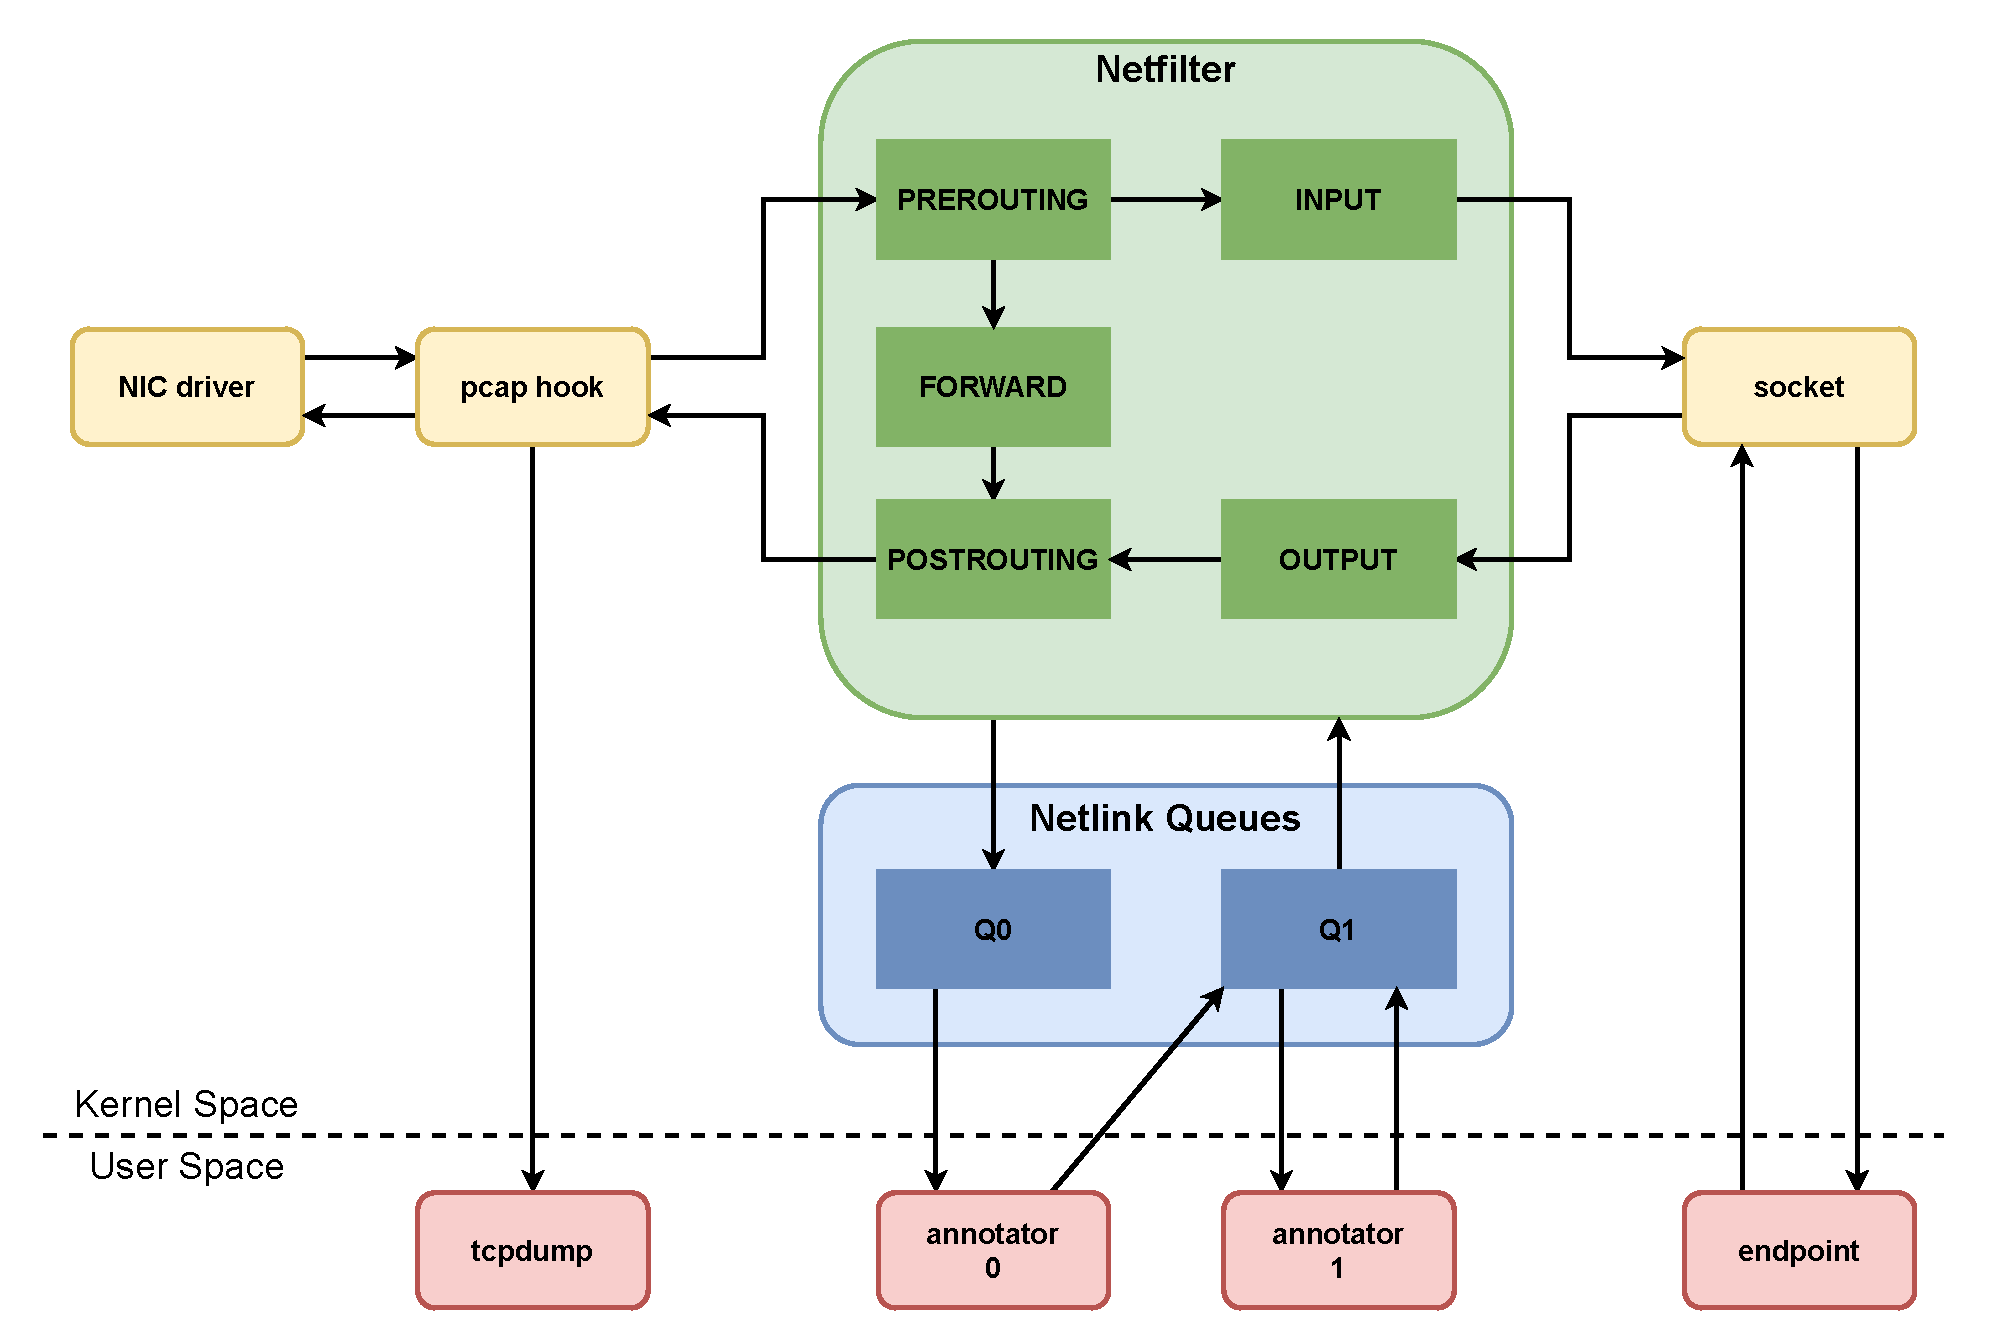
\includegraphics[width=\textwidth,keepaspectratio]{figures/netfilter_queue.pdf}
    \caption{Packet data path when matching an iptables rule with a NFQUEUE target}
    \label{extend:ops:fig:nfq}
\end{figure}

Specifically, once a packet reaches a Netfilter hook that corresponds to one of the main five chains (i.e., PREROUTING, INPUT, etc.) and satisfies the match criteria of a specific \texttt{iptables} rule, the packet is enqueued, pending further analysis. After a userspace process subscribes to the very same queue, the packet is copied to its virtual address space, starting with its Layer 3 header, via a Unix Domain Socket. The process is allowed to inspect the packet, and even to further buffer it while requesting subsequent matches for out-of-order processing. Eventually, a verdict must be reached and communicated to the kernel as one of the standard terminal targets in \texttt{iptables} (e.g., ACCEPT, DROP, etc.)

The reason this extension is useful to us is not necessarily the filtration aspect, but the fact that once the verdict has been established, the process can supply a modified version of the packet. This new packet will overwrite the one initially captured by the Netfilter hook. Given a positive verdict, the modified packet will be reinserted into the network stack, following the intended data path and reaching its endpoint. Note, however, that the userspace process can additionally specify another queue to be used for reinsertion. If this is indeed the case, the potentially modified packet will be stalled once again for analysis. The process performing the second inspection (i.e., the process subscribed to the second queue) does not necessarily need to be the same process as before.

\subsubsection{Annotation tool}
\label{extend:ops:architecture:annotation}

In testing different features of Layer 3 and Layer 4 protocols, a usual approach consists of generating synthetic traffic and bypassing the network stack of the originating host. We decided to forgo this method in favor of a more practical alternative: modifying real traffic. The primary advantage of the latter scheme over the former is the ability to verify not only that the annotated packets can be successfully transmitted over the network, but also that their alteration does not impact higher level protocols in the OSI stack. Additionally, the flexibility in assessing compliance with stateful firewalls alleviates the effort that would have otherwise been required to simulate sufficiently credible sessions.

These aspects gave impetus to the development of a method to insert multiple protocol specific options in outgoing traffic. One of the essential characteristics of the resulting tool is the capacity to easily implement new options for existing protocols or to register new protocols altogether. Limited by the extent of our needs for this experiment, session tracking falls outside its purview. As a result, options such as MultiPath TCP are not available for testing. Instead, all options should either be static in nature (e.g., NOP) or depend entirely on the information available in a single packet's header and payload (e.g., alternative checksums). Otherwise, its use may be limited to determining only whether the initial packet was able to traverse the network (e.g., TCP timestamps).

\begin{algorithm}[h]
    \caption{Packet annotation algorithm}
    \label{extend:ops:alg:annotator}
    \begin{algorithmic}[1]
        \State \textbf{Input:} $user\_codepoints[n]$, $user\_proto$, NFQ packet stream
        \State \textbf{Output:} modified packets
        \item[]

        \Function{process\_packet}{$pkt$}
            \If{$pkt.proto \neq user\_proto$}
                \State \Return{$pkt$}
            \EndIf
            \item[]

            \State \textcolor{gray}{// Step 1: Options decoding}
            \State $ops\_buff \gets \epsilon$
            \For{\textbf{each} $codepoint$ \textbf{in} $user\_codepoints$}
                \State $ops\_buff \gets ops\_buff$ $\cup$ \Call{expand}{codepoint}
            \EndFor
            \item[]

            \State \textcolor{gray}{// Step 2: Packet reassembly}
            \If{should replace options}
                \State $pkt.ops \gets \epsilon$
            \EndIf
            \State $pkt.ops \gets pkt.ops$ $\cup$ $ops\_buff$
            \State \Call{adjust\_hdr\_lengths}{$pkt$}
            \item[]

            \State \textcolor{gray}{// Step 3: Checksum recalculation}
            \State \Call{recalculate\_csums}{$pkt$}
            \item[]

            \State \Return $pkt$
        \EndFunction
    \end{algorithmic}
\end{algorithm}

Next, we present a summary overview of the tool's operation. Initially, the user adds one or more \texttt{iptables} rules with an \texttt{NFQUEUE} target. All packets that match one of these rules are redirected into userspace for our tool to evaluate and modify as it sees fit. During the initial invocation of the tool, the user may specify a sequence of bytes that represent option codepoints. For each packet, the codepoints will be expanded to actual TLV entries and inserted into a (potentially new) options section. The NetfilterQueue callback that fulfils this purpose takes three steps towards successful annotation. These steps are summarily described in Algorithm \ref{extend:ops:alg:annotator} and further explained below.

\textbf{Options Decoding:} having access to the packet, as provided by the Netfilter kernel hook, the first step is generating the contents of the options section for a pre-established protocol (i.e., IP, TCP, UDP). Using the user-specified sequence of \texttt{option-type} octets, specific decoder functions are called upon to expand them, thus populating the options buffer. This expansion phase is by and large an arbitrary process. For example, an IP Timestamp Option (\texttt{0x44}) will be translated to a 12 octet buffer containing a single timestamp associated to the source IP address. The generated flags will denote pre-specified address fields as to discourage addition of new timestamps from compliant middleboxes. This inhibition of user agency is a conscious decision intended to simplify the tool's usage. Nonetheless, the decoder functions can be easily modified on a case-by-case basis to accept more information and conform to finer-grained requirements. Note that the options will appear in the order in which they were initially specified by the user. However, the order in which they are generated may vary. For example, a UDP Options Checksum (\texttt{0x02}) is supposed to be placed as close to the beginning of the section as possible, while at the same time requiring all other options to have already been calculated. Consequently, it's decoding is delayed based on a discretionary option priority assignment.

\textbf{Packet Reassembly:} This step modifies the initial packet in order to include the newly generated options. Any related fields (e.g., \texttt{IP.total\_length}) with the exception of the checksum are adjusted to account for the payload offset. Based on user preference, existing options can either be completely replaced, or preserved. In our tests, we employed the former approach in order to exert full control over the content of the options section. Alternatively, existing options would take precedence. In turn, this could lead to overflowing user-specified options to be discarded due to space constraints.

\textbf{Checksum Recalculation:} The reason why this step is separate from the previous is that changes made to a header corresponding to a lower layer can impact the checksum of a higher layer protocol. For example, while IP options are intended to extend only the IP header, the total packet length increases nonetheless. As a result, TCP's or UDP's pseudo-header changes and the Layer 4 checksum does so along with it.

An advantage of relying on the Netfilter framework is that it integrates well with \texttt{ip-xfrm} (kernel-side module that implements the IPsec protocol suite). Usually, VPN implementations are split across both userspace and kernelspace. The former carries out the negotiation required as per the IKE protocol, which establishes up to four Security Associations (SA) and creates a Security Policy (SP). The latter utilizes the SAs for packet encapsulation and encryption but more importantly, it uses the SP to determine which packets are to be passed to the IPsec stack. This decision is taken by consulting an SP database after the packet has traversed the \texttt{OUTPUT} and \texttt{POSTROUTING} chains. If appropriate, the packet is modified and reinserted prior to entering the \texttt{OUTPUT} chain. The \texttt{iptables} rule that identifies the packets which require annotations must be well-defined. Otherwise, the user risks modifying a packet that is protected by the ESP protocol. We consider this approach preferable to excluding packets containing ESP headers. Due to the potential usage of NAT-traversal encapsulation, it would be inefficient to identify the presence of the ESP header. Moreover, allowing UDP packets with destination port 4500 to pass may exempt IKE configuration packets from annotation, contrary to the user's intention.

\subsubsection{Testing framework}
\label{extend:ops:architecture:cloud}

Irrespective of the type of protocol that may benefit from these extensions, they will in all likelihood be required to interact with cloud-hosted solutions \cite{daielephant}. As a result, we focus our efforts on verifying if and how cloud providers allow the passage of annotated packets through their networks. To this end, we perform a series of inter-regional tests. The structure of the testing environment can be seen in Fig. \ref{extend:ops:fig:architecture}. Initially, the management instance (i.e., localhost) will install the annotation tool, as well as any traffic generation tools under test on each virtual machine. Additionally it will also start \texttt{tcpdump} processes and insert specific \texttt{iptables} rules with the purpose capturing relevant traffic for annotation and later analysis. When testing a certain instance (e.g., the one in me-south-1 region in AWS), a server will be started (1) by issuing a command over a ssh channel. Immediately after, all other instances will be issued similar commands, to start a client (2) and send requests to the server. The resulting traffic will be annotated in both directions. After all communication (3) will have ceased, another instance will be selected as the server. Finally, all \texttt{tcpdump} processes will be killed and the generated packet captures as well as any logs will be downloaded for analysis.

\begin{figure}[htb]
    \centering
    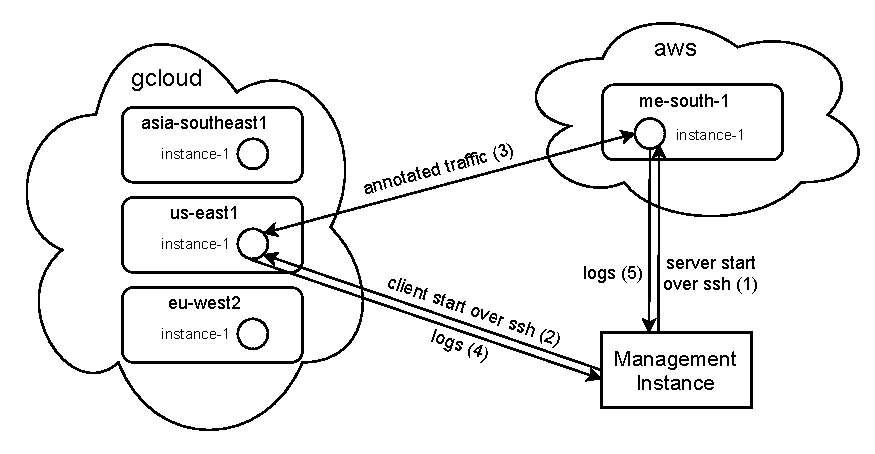
\includegraphics[width=\textwidth,keepaspectratio]{figures/architecture.pdf}
    \caption{Architecture of the cloud testing framework.}
    \label{extend:ops:fig:architecture}
\end{figure}

The framework is comprised mostly of bash scripts using each provider's CLI management tool. A minimal setup is required: configuring default projects and public keys, enabling billing, and relaxing the firewall rules of their private networks to the extent that they are permitted. The scripts can be classified as management scripts, experiment scripts or analysis scripts, depending on their purpose. Management scripts allow the automatic creation or deletion of VM instances in accordance with a pre-specified list of regions. This list can be freely modified in accordance with the available selection of each cloud provider. Additionally, they administer the configuration of VPNs or that of the annotation tool. Experiment scripts install missing dependencies and generate traffic between any two instances. The commands executed on remote machines are issued over a secure SSH channel. All relevant inbound and outbound traffic is recorded on each instance and eventually imported on the managing host. Any analysis of packet reception and option removal or alteration can be done offline. To this end, we offer a subset of the analysis scripts that we employed in interpreting the network captures, along with samples of said captures. We include only general-purpose scripts that, for example, report overall instance reachability or retrieve AS numbers and names of recorded IP addresses.

Note that this framework is not specifically aimed at evaluating cloud providers. Their preponderance in our tests was meant to verify the compliance to the protocol extension standards in the wider Internet. Given that the credentials are correctly configured on all machines, the experiments can be executed with either a statically defined set of public and private IPs, or via a user-provided means of dynamically generating said set.

%%%%%%%%%%%%%%%%%%%%%%%%%%%%%%%%%%%%%%%%%%%%%%%%%%%%%%%%%%%%%%%%%%%%%%%%%%%%%%%%
\subsection{Evaluation}
\label{extend:ops:evaluation}

Our experimental setup consisted of twenty virtual machines, spawned in five different regions per each tested cloud provider. The principal criterion that influenced our choice of regions was geographical diversity, both within the same provider's selection and across all instances. As a result, regions that were uniquely available from a certain provider (e.g., Middle East) took priority over the more common ones (e.g., Europe). Each instance ran the default Ubuntu 18.04 image offered by its corresponding provider and was allocated 1-2vCPUs, 1-4GB RAM (depending on the available flavors) and a public IP address. In addition to these, we also included a Ubuntu 20.04 VM instance running on our personal server, over VMware vSphere 7 and behind a Palo Alto 5540 Firewall. During our tests, we established over 50k connections over a period of approximately three weeks. Due to the resulting overall cost of US\$150, we consider that our framework usable in repeated testing.

The experiments themselves consisted of sequentially selecting an instance from the available pool and transmitting annotated traffic from all other sources. For IP options, the protocols that we tested were ICMP (Echo Request), DNS and NTP over UDP, FTP, HTTP and TCP-FastOpen over TCP, as well as raw data on arbitrarily chosen free ephemeral ports (using both UDP and TCP). UDP and TCP options were similarly tested over their respective subgroups from the previously stated selection. A complete account of all tested options can be found in Table \ref{extend:ops:table:ops-acceptance}, as well as their respective acceptance rating, grouped by cloud provider. The "Received by" section, for example, represents the amount of unaltered, annotated traffic that reached instances belonging to a certain provider. This includes experiments initiated from different regions of the same provider. For instance, an IP Record Route value of 3.25\% for AWS is relative to five instances per cloud provider, twenty sets of experiments initiated by other hosts per instance, and 8 experiments testing different higher layer protocols per set. We note that in some cases (e.g., IP Timestamp option) we conducted more than twenty sets of experiments per instance, in order to obtain sufficient data for other forms of analysis. Consequently, the results are averaged across these batches of experiments. Note that each experiment focuses on a single option at a time; due to limited resources, we do not test combinations of options.

\begin{table*}[t]
    \centering
    \caption{Percentage of annotated traffic received \textit{from} any other host and \textit{by} any other host. Grouped by option type and averaged per provider. Data collected from multiple types of experiments (expts).}
    \label{extend:ops:table:ops-acceptance}
    \begin{adjustbox}{max width=\textwidth}
    \begin{tabular}{|c|c|c|c|c|c|c|c|c|c|c|c|}
        \hline
        %% ROW 1
        \multirow{3}{*}{\vtop{\hbox{\strut Protocol}\hbox{\strut (expts)}}}
        & \multirow{3}{*}{Option}
        & \multicolumn{10}{c|}{Acceptance Rate (\%)} \\
        \hhline{~~*{10}{-}}
        %% ROW 2
        & & \multicolumn{5}{c|}{Received by} 
          & \multicolumn{5}{c|}{Received from} \\
        \hhline{~~*{10}{-}}
        %% ROW 3
        & & gcloud & aws & azure & docean & personal 
          & gcloud & aws & azure & docean & personal  \\
        \hline
        %% IP ops group
        \multirow{5}{*}{IP (8)}
        % avg: dns, ftp, http, _________ x2, ntp, ping, tfo
        & 4x NOP       & 0 & 3.00 & 0 & 5.50 & 4.37 & 1.50 & 1.75 & 1.00 & 4.25 & 4.37 \\
        % avg: ___, ___, http, _________ x2, ntp, ping, ___
        & Record Route & 0 & 3.25 & 0 & 6.00 & 5.00 & 1.37 & 1.75 & 2.00 & 4.25 & 4.37 \\
        % > avg: dns, ___, http, nc-80-123 x2, ntp, ping, ___ 
        & Timestamp    & 0 & 3.08 & 0 & 5.91 & 4.37 & 2.00 & 1.75 & 1.00 & 4.25 & 4.37 \\
        % avg: dns, ftp, http, _________ x2, ntp, ping, tfo
        & Experimental & 0 & 2.75 & 0 & 5.75 & 0 & 1.50 & 1.50 & 0.87 & 3.75 & 4.37 \\
        % avg: dns, ftp, http, _________ x2, ntp, ping, tfo
        & Unassigned   & 0 & 2.75 & 0 & 4.87 & 0 & 1.50 & 1.50 & 0 & 3.75 & 4.37 \\
        \hline
        %% TCP ops group
        \multirow{6}{*}{TCP (4)}
        % avg: ftp, http, nc-random, tfo
        & 4x NOP       & 100 & 100 & 100 & 100 & 100 & 100 & 100 & 100 & 100 & 100 \\
        % avg: ftp, http, nc-random, tfo
        & Echo         & 100 & 100 & 100 & 100 & 100 & 100 & 100 & 100 & 100 & 100 \\
        % avg: ftp, http, nc-random, tfo
        & Echo-Reply   & 100 & 100 & 100 & 100 & 100 & 100 & 100 & 100 & 100 & 100 \\
        % avg: ___, http, _________, tfo
        & Timestamp    & 100 & 100 & 100 & 100 & 100 & 100 & 100 & 100 & 100 & 100 \\
        % avg: ftp, http, nc-random, tfo
        & Experimental & 100 & 100 & 100 & 100 & 100 & 100 & 100 & 100 & 100 & 100 \\
        % avg: ftp, http, nc-random, tfo
        & Reserved     & 100 & 100 & 100 & 100 & 100 & 100 & 100 & 100 & 100 & 100 \\
        \hline
        %% UDP ops group
        \multirow{8}{*}{UDP (3)}
        % avg: dns, ntp, nc-rnadom
        & 4x NOP             & 0 & 68.00 & 75.00 & 75.00 & 73.33 & 0 & 74.83 & 72.00 & 71.33 & 72.50 \\
        % avg: dns, ntp, nc-rnadom
        % NOTE: between google and aws, unassigned-cc-1 passed with option removed
        & 4x NOP \& CCO       & 0 & 68.50 & 75.00 & 74.83 & 73.33 & 0 & 74.66 & 72.50 & 71.33 & 72.50 \\
        % avg: dns, ntp, nc-rnadom
        & Timestamp          & 0 & 72.50 & 74.83 & 74.66 & 74.16 & 0 & 75.00 & 74.50 & 72.33 & 75.00 \\
        % avg: dns, ntp, nc-rnadom
        & Timestamp \& CCO    & 0 & 72.16 & 74.66 & 72.33 & 75.00 & 0 & 74.16 & 73.66 & 71.50 & 74.16 \\
        % avg: dns, ntp, nc-rnadom
        & Experimental       & 0 & 72.50 & 75.00 & 75.00 & 75.00 & 0 & 75.00 & 74.50 & 73.00 & 75.00 \\
        % avg: dns, ntp, nc-rnadom
        & Experimental \& CCO & 0 & 72.50 & 75.00 & 75.00 & 75.00 & 0 & 75.00 & 74.50 & 73.00 & 75.00 \\
        % avg: dns, ntp, nc-rnadom
        & Unassigned         & 0 & 72.50 & 75.00 & 75.00 & 75.00 & 0 & 75.00 & 74.50 & 73.00 & 75.00 \\
        % avg: dns, ntp, nc-rnadom
        & Unassigned \& CCO   & 0 & 72.50 & 75.50 & 75.00 & 74.16 & 0 & 75.00 & 74.50 & 72.16 & 75.00 \\
        \hline
    \end{tabular}
    \end{adjustbox}
\end{table*}


For all protocols, we included a test consisting of four consecutive NOPs (No Options). Normally this option is used as padding in solving alignment issues. However, no more than three NOPs would be required if this was indeed the case. Four or more NOPs could either indicate that options had been purposefully removed during the network traversal by middleboxes, or they could be construed as a relatively weak DoS attack meant to exhaust CPU cycles by means of processing inconsequential options. Due to this ambiguity, we surmised that firewall manufacturers may prove less lenient towards such occurrences. Nonetheless, our tests revealed that the 4xNOP case did not impede communication in instances where other options lead to successful network traversals, regardless of protocol.

As one of our leading goals, we resolved to verify not only the acceptance of well-established options, but also that of unassigned or reserved ones. Similarly to the four NOP case, an undefined option can also be evaluated as malicious. While the former could be motivated by the arbitrary removal of interspersed options by routers, the latter could be considered a less ambiguous attempt at a DoS by certain firewalls \cite{I-D.ietf-tsvwg-udp-options}. Consequently we implemented two variations of an undefined option. The first option utilizes an unassigned or a IANA-reserved codepoint for each protocol (IP: \texttt{0x5d}, TCP: \texttt{0x47}, UDP: \texttt{0x7d}) which fills the data field with consecutively-valued data bytes until the next 32-bit boundary in the options section. The second option is implemented almost identically. The only difference is that it follows the recommendation on shared use of 16-bit experimental IDs and uses the \texttt{0xfe} codepoint for both the TCP and UDP instantiation.

In the following subsections we discuss each IP, TCP and UDP option that we tested, identifying practical applications and deciding their suitability for large scale deployment.


\subsubsection{Analysis of IP options}
\label{extend:ops:evaluation:ip-ops}

After testing multiple IP options in combination with different transport layer protocols, we concluded that with the exception of ICMP messages, all packets are consistently dropped. For this reason, our following analysis will focus primarily on the idiosyncratic behaviour of certain providers towards each of the examined options.

\textbf{Timestamp option.} Consists of a 4-byte header, followed by a data segment of arbitrary length. The header fields are as follow: Option Type and Option Length (adhering to the TLV encoding of most options), succeeded by a one-byte Pointer field denoting the offset into the option where a host may add a new timestamp, and two nibble-sized Overflow and Flag fields. The Overflow field is set initially to zero and is incremented by each host that is willing but unable to add a timestamp. The Flag field defines multiple modes of operation: the hosts are either required to append only 32-bit timestamps, or to add the IP of the corresponding interface as well. In case of the latter, multiple IPs can be pre-specified so that only select hosts may add their timestamps. Initially, we crafted packets such that they contained only the originating host's IP and timestamp, while no middleboxes would be allowed to append their own. The reason for this was to easily verify if the contents of the option could be modified in transit, given that the packets ever reached their destination. Later, we relaxed this constraint and allowed middleboxes to add their own timestamps, which did not give rise to any new impediments.

\begin{figure}[htb]
        % \hbox{\centering \scalebox{1.0}{%% Creator: Matplotlib, PGF backend
%%
%% To include the figure in your LaTeX document, write
%%   \input{<filename>.pgf}
%%
%% Make sure the required packages are loaded in your preamble
%%   \usepackage{pgf}
%%
%% Figures using additional raster images can only be included by \input if
%% they are in the same directory as the main LaTeX file. For loading figures
%% from other directories you can use the `import` package
%%   \usepackage{import}
%% and then include the figures with
%%   \import{<path to file>}{<filename>.pgf}
%%
%% Matplotlib used the following preamble
%%
\begingroup%
\makeatletter%
\begin{pgfpicture}%
\pgfpathrectangle{\pgfpointorigin}{\pgfqpoint{6.400000in}{4.800000in}}%
\pgfusepath{use as bounding box, clip}%
\begin{pgfscope}%
\pgfsetbuttcap%
\pgfsetmiterjoin%
\definecolor{currentfill}{rgb}{1.000000,1.000000,1.000000}%
\pgfsetfillcolor{currentfill}%
\pgfsetlinewidth{0.000000pt}%
\definecolor{currentstroke}{rgb}{1.000000,1.000000,1.000000}%
\pgfsetstrokecolor{currentstroke}%
\pgfsetdash{}{0pt}%
\pgfpathmoveto{\pgfqpoint{0.000000in}{0.000000in}}%
\pgfpathlineto{\pgfqpoint{6.400000in}{0.000000in}}%
\pgfpathlineto{\pgfqpoint{6.400000in}{4.800000in}}%
\pgfpathlineto{\pgfqpoint{0.000000in}{4.800000in}}%
\pgfpathclose%
\pgfusepath{fill}%
\end{pgfscope}%
\begin{pgfscope}%
\pgfsetbuttcap%
\pgfsetmiterjoin%
\definecolor{currentfill}{rgb}{1.000000,1.000000,1.000000}%
\pgfsetfillcolor{currentfill}%
\pgfsetlinewidth{0.000000pt}%
\definecolor{currentstroke}{rgb}{0.000000,0.000000,0.000000}%
\pgfsetstrokecolor{currentstroke}%
\pgfsetstrokeopacity{0.000000}%
\pgfsetdash{}{0pt}%
\pgfpathmoveto{\pgfqpoint{0.800000in}{0.528000in}}%
\pgfpathlineto{\pgfqpoint{5.760000in}{0.528000in}}%
\pgfpathlineto{\pgfqpoint{5.760000in}{4.224000in}}%
\pgfpathlineto{\pgfqpoint{0.800000in}{4.224000in}}%
\pgfpathclose%
\pgfusepath{fill}%
\end{pgfscope}%
\begin{pgfscope}%
\pgfsetbuttcap%
\pgfsetroundjoin%
\definecolor{currentfill}{rgb}{0.000000,0.000000,0.000000}%
\pgfsetfillcolor{currentfill}%
\pgfsetlinewidth{0.803000pt}%
\definecolor{currentstroke}{rgb}{0.000000,0.000000,0.000000}%
\pgfsetstrokecolor{currentstroke}%
\pgfsetdash{}{0pt}%
\pgfsys@defobject{currentmarker}{\pgfqpoint{0.000000in}{-0.048611in}}{\pgfqpoint{0.000000in}{0.000000in}}{%
\pgfpathmoveto{\pgfqpoint{0.000000in}{0.000000in}}%
\pgfpathlineto{\pgfqpoint{0.000000in}{-0.048611in}}%
\pgfusepath{stroke,fill}%
}%
\begin{pgfscope}%
\pgfsys@transformshift{0.903333in}{0.528000in}%
\pgfsys@useobject{currentmarker}{}%
\end{pgfscope}%
\end{pgfscope}%
\begin{pgfscope}%
\definecolor{textcolor}{rgb}{0.000000,0.000000,0.000000}%
\pgfsetstrokecolor{textcolor}%
\pgfsetfillcolor{textcolor}%
\pgftext[x=0.903333in,y=0.430778in,,top]{\color{textcolor}\rmfamily\fontsize{12.000000}{14.400000}\selectfont 1}%
\end{pgfscope}%
\begin{pgfscope}%
\pgfsetbuttcap%
\pgfsetroundjoin%
\definecolor{currentfill}{rgb}{0.000000,0.000000,0.000000}%
\pgfsetfillcolor{currentfill}%
\pgfsetlinewidth{0.803000pt}%
\definecolor{currentstroke}{rgb}{0.000000,0.000000,0.000000}%
\pgfsetstrokecolor{currentstroke}%
\pgfsetdash{}{0pt}%
\pgfsys@defobject{currentmarker}{\pgfqpoint{0.000000in}{-0.048611in}}{\pgfqpoint{0.000000in}{0.000000in}}{%
\pgfpathmoveto{\pgfqpoint{0.000000in}{0.000000in}}%
\pgfpathlineto{\pgfqpoint{0.000000in}{-0.048611in}}%
\pgfusepath{stroke,fill}%
}%
\begin{pgfscope}%
\pgfsys@transformshift{1.110000in}{0.528000in}%
\pgfsys@useobject{currentmarker}{}%
\end{pgfscope}%
\end{pgfscope}%
\begin{pgfscope}%
\definecolor{textcolor}{rgb}{0.000000,0.000000,0.000000}%
\pgfsetstrokecolor{textcolor}%
\pgfsetfillcolor{textcolor}%
\pgftext[x=1.110000in,y=0.430778in,,top]{\color{textcolor}\rmfamily\fontsize{12.000000}{14.400000}\selectfont 2}%
\end{pgfscope}%
\begin{pgfscope}%
\pgfsetbuttcap%
\pgfsetroundjoin%
\definecolor{currentfill}{rgb}{0.000000,0.000000,0.000000}%
\pgfsetfillcolor{currentfill}%
\pgfsetlinewidth{0.803000pt}%
\definecolor{currentstroke}{rgb}{0.000000,0.000000,0.000000}%
\pgfsetstrokecolor{currentstroke}%
\pgfsetdash{}{0pt}%
\pgfsys@defobject{currentmarker}{\pgfqpoint{0.000000in}{-0.048611in}}{\pgfqpoint{0.000000in}{0.000000in}}{%
\pgfpathmoveto{\pgfqpoint{0.000000in}{0.000000in}}%
\pgfpathlineto{\pgfqpoint{0.000000in}{-0.048611in}}%
\pgfusepath{stroke,fill}%
}%
\begin{pgfscope}%
\pgfsys@transformshift{1.316667in}{0.528000in}%
\pgfsys@useobject{currentmarker}{}%
\end{pgfscope}%
\end{pgfscope}%
\begin{pgfscope}%
\definecolor{textcolor}{rgb}{0.000000,0.000000,0.000000}%
\pgfsetstrokecolor{textcolor}%
\pgfsetfillcolor{textcolor}%
\pgftext[x=1.316667in,y=0.430778in,,top]{\color{textcolor}\rmfamily\fontsize{12.000000}{14.400000}\selectfont 3}%
\end{pgfscope}%
\begin{pgfscope}%
\pgfsetbuttcap%
\pgfsetroundjoin%
\definecolor{currentfill}{rgb}{0.000000,0.000000,0.000000}%
\pgfsetfillcolor{currentfill}%
\pgfsetlinewidth{0.803000pt}%
\definecolor{currentstroke}{rgb}{0.000000,0.000000,0.000000}%
\pgfsetstrokecolor{currentstroke}%
\pgfsetdash{}{0pt}%
\pgfsys@defobject{currentmarker}{\pgfqpoint{0.000000in}{-0.048611in}}{\pgfqpoint{0.000000in}{0.000000in}}{%
\pgfpathmoveto{\pgfqpoint{0.000000in}{0.000000in}}%
\pgfpathlineto{\pgfqpoint{0.000000in}{-0.048611in}}%
\pgfusepath{stroke,fill}%
}%
\begin{pgfscope}%
\pgfsys@transformshift{1.523333in}{0.528000in}%
\pgfsys@useobject{currentmarker}{}%
\end{pgfscope}%
\end{pgfscope}%
\begin{pgfscope}%
\definecolor{textcolor}{rgb}{0.000000,0.000000,0.000000}%
\pgfsetstrokecolor{textcolor}%
\pgfsetfillcolor{textcolor}%
\pgftext[x=1.523333in,y=0.430778in,,top]{\color{textcolor}\rmfamily\fontsize{12.000000}{14.400000}\selectfont 4}%
\end{pgfscope}%
\begin{pgfscope}%
\pgfsetbuttcap%
\pgfsetroundjoin%
\definecolor{currentfill}{rgb}{0.000000,0.000000,0.000000}%
\pgfsetfillcolor{currentfill}%
\pgfsetlinewidth{0.803000pt}%
\definecolor{currentstroke}{rgb}{0.000000,0.000000,0.000000}%
\pgfsetstrokecolor{currentstroke}%
\pgfsetdash{}{0pt}%
\pgfsys@defobject{currentmarker}{\pgfqpoint{0.000000in}{-0.048611in}}{\pgfqpoint{0.000000in}{0.000000in}}{%
\pgfpathmoveto{\pgfqpoint{0.000000in}{0.000000in}}%
\pgfpathlineto{\pgfqpoint{0.000000in}{-0.048611in}}%
\pgfusepath{stroke,fill}%
}%
\begin{pgfscope}%
\pgfsys@transformshift{1.730000in}{0.528000in}%
\pgfsys@useobject{currentmarker}{}%
\end{pgfscope}%
\end{pgfscope}%
\begin{pgfscope}%
\definecolor{textcolor}{rgb}{0.000000,0.000000,0.000000}%
\pgfsetstrokecolor{textcolor}%
\pgfsetfillcolor{textcolor}%
\pgftext[x=1.730000in,y=0.430778in,,top]{\color{textcolor}\rmfamily\fontsize{12.000000}{14.400000}\selectfont 5}%
\end{pgfscope}%
\begin{pgfscope}%
\pgfsetbuttcap%
\pgfsetroundjoin%
\definecolor{currentfill}{rgb}{0.000000,0.000000,0.000000}%
\pgfsetfillcolor{currentfill}%
\pgfsetlinewidth{0.803000pt}%
\definecolor{currentstroke}{rgb}{0.000000,0.000000,0.000000}%
\pgfsetstrokecolor{currentstroke}%
\pgfsetdash{}{0pt}%
\pgfsys@defobject{currentmarker}{\pgfqpoint{0.000000in}{-0.048611in}}{\pgfqpoint{0.000000in}{0.000000in}}{%
\pgfpathmoveto{\pgfqpoint{0.000000in}{0.000000in}}%
\pgfpathlineto{\pgfqpoint{0.000000in}{-0.048611in}}%
\pgfusepath{stroke,fill}%
}%
\begin{pgfscope}%
\pgfsys@transformshift{1.936667in}{0.528000in}%
\pgfsys@useobject{currentmarker}{}%
\end{pgfscope}%
\end{pgfscope}%
\begin{pgfscope}%
\definecolor{textcolor}{rgb}{0.000000,0.000000,0.000000}%
\pgfsetstrokecolor{textcolor}%
\pgfsetfillcolor{textcolor}%
\pgftext[x=1.936667in,y=0.430778in,,top]{\color{textcolor}\rmfamily\fontsize{12.000000}{14.400000}\selectfont 6}%
\end{pgfscope}%
\begin{pgfscope}%
\pgfsetbuttcap%
\pgfsetroundjoin%
\definecolor{currentfill}{rgb}{0.000000,0.000000,0.000000}%
\pgfsetfillcolor{currentfill}%
\pgfsetlinewidth{0.803000pt}%
\definecolor{currentstroke}{rgb}{0.000000,0.000000,0.000000}%
\pgfsetstrokecolor{currentstroke}%
\pgfsetdash{}{0pt}%
\pgfsys@defobject{currentmarker}{\pgfqpoint{0.000000in}{-0.048611in}}{\pgfqpoint{0.000000in}{0.000000in}}{%
\pgfpathmoveto{\pgfqpoint{0.000000in}{0.000000in}}%
\pgfpathlineto{\pgfqpoint{0.000000in}{-0.048611in}}%
\pgfusepath{stroke,fill}%
}%
\begin{pgfscope}%
\pgfsys@transformshift{2.143333in}{0.528000in}%
\pgfsys@useobject{currentmarker}{}%
\end{pgfscope}%
\end{pgfscope}%
\begin{pgfscope}%
\definecolor{textcolor}{rgb}{0.000000,0.000000,0.000000}%
\pgfsetstrokecolor{textcolor}%
\pgfsetfillcolor{textcolor}%
\pgftext[x=2.143333in,y=0.430778in,,top]{\color{textcolor}\rmfamily\fontsize{12.000000}{14.400000}\selectfont 7}%
\end{pgfscope}%
\begin{pgfscope}%
\pgfsetbuttcap%
\pgfsetroundjoin%
\definecolor{currentfill}{rgb}{0.000000,0.000000,0.000000}%
\pgfsetfillcolor{currentfill}%
\pgfsetlinewidth{0.803000pt}%
\definecolor{currentstroke}{rgb}{0.000000,0.000000,0.000000}%
\pgfsetstrokecolor{currentstroke}%
\pgfsetdash{}{0pt}%
\pgfsys@defobject{currentmarker}{\pgfqpoint{0.000000in}{-0.048611in}}{\pgfqpoint{0.000000in}{0.000000in}}{%
\pgfpathmoveto{\pgfqpoint{0.000000in}{0.000000in}}%
\pgfpathlineto{\pgfqpoint{0.000000in}{-0.048611in}}%
\pgfusepath{stroke,fill}%
}%
\begin{pgfscope}%
\pgfsys@transformshift{2.350000in}{0.528000in}%
\pgfsys@useobject{currentmarker}{}%
\end{pgfscope}%
\end{pgfscope}%
\begin{pgfscope}%
\definecolor{textcolor}{rgb}{0.000000,0.000000,0.000000}%
\pgfsetstrokecolor{textcolor}%
\pgfsetfillcolor{textcolor}%
\pgftext[x=2.350000in,y=0.430778in,,top]{\color{textcolor}\rmfamily\fontsize{12.000000}{14.400000}\selectfont 8}%
\end{pgfscope}%
\begin{pgfscope}%
\pgfsetbuttcap%
\pgfsetroundjoin%
\definecolor{currentfill}{rgb}{0.000000,0.000000,0.000000}%
\pgfsetfillcolor{currentfill}%
\pgfsetlinewidth{0.803000pt}%
\definecolor{currentstroke}{rgb}{0.000000,0.000000,0.000000}%
\pgfsetstrokecolor{currentstroke}%
\pgfsetdash{}{0pt}%
\pgfsys@defobject{currentmarker}{\pgfqpoint{0.000000in}{-0.048611in}}{\pgfqpoint{0.000000in}{0.000000in}}{%
\pgfpathmoveto{\pgfqpoint{0.000000in}{0.000000in}}%
\pgfpathlineto{\pgfqpoint{0.000000in}{-0.048611in}}%
\pgfusepath{stroke,fill}%
}%
\begin{pgfscope}%
\pgfsys@transformshift{2.556667in}{0.528000in}%
\pgfsys@useobject{currentmarker}{}%
\end{pgfscope}%
\end{pgfscope}%
\begin{pgfscope}%
\definecolor{textcolor}{rgb}{0.000000,0.000000,0.000000}%
\pgfsetstrokecolor{textcolor}%
\pgfsetfillcolor{textcolor}%
\pgftext[x=2.556667in,y=0.430778in,,top]{\color{textcolor}\rmfamily\fontsize{12.000000}{14.400000}\selectfont 9}%
\end{pgfscope}%
\begin{pgfscope}%
\pgfsetbuttcap%
\pgfsetroundjoin%
\definecolor{currentfill}{rgb}{0.000000,0.000000,0.000000}%
\pgfsetfillcolor{currentfill}%
\pgfsetlinewidth{0.803000pt}%
\definecolor{currentstroke}{rgb}{0.000000,0.000000,0.000000}%
\pgfsetstrokecolor{currentstroke}%
\pgfsetdash{}{0pt}%
\pgfsys@defobject{currentmarker}{\pgfqpoint{0.000000in}{-0.048611in}}{\pgfqpoint{0.000000in}{0.000000in}}{%
\pgfpathmoveto{\pgfqpoint{0.000000in}{0.000000in}}%
\pgfpathlineto{\pgfqpoint{0.000000in}{-0.048611in}}%
\pgfusepath{stroke,fill}%
}%
\begin{pgfscope}%
\pgfsys@transformshift{2.763333in}{0.528000in}%
\pgfsys@useobject{currentmarker}{}%
\end{pgfscope}%
\end{pgfscope}%
\begin{pgfscope}%
\definecolor{textcolor}{rgb}{0.000000,0.000000,0.000000}%
\pgfsetstrokecolor{textcolor}%
\pgfsetfillcolor{textcolor}%
\pgftext[x=2.763333in,y=0.430778in,,top]{\color{textcolor}\rmfamily\fontsize{12.000000}{14.400000}\selectfont 10}%
\end{pgfscope}%
\begin{pgfscope}%
\pgfsetbuttcap%
\pgfsetroundjoin%
\definecolor{currentfill}{rgb}{0.000000,0.000000,0.000000}%
\pgfsetfillcolor{currentfill}%
\pgfsetlinewidth{0.803000pt}%
\definecolor{currentstroke}{rgb}{0.000000,0.000000,0.000000}%
\pgfsetstrokecolor{currentstroke}%
\pgfsetdash{}{0pt}%
\pgfsys@defobject{currentmarker}{\pgfqpoint{0.000000in}{-0.048611in}}{\pgfqpoint{0.000000in}{0.000000in}}{%
\pgfpathmoveto{\pgfqpoint{0.000000in}{0.000000in}}%
\pgfpathlineto{\pgfqpoint{0.000000in}{-0.048611in}}%
\pgfusepath{stroke,fill}%
}%
\begin{pgfscope}%
\pgfsys@transformshift{2.970000in}{0.528000in}%
\pgfsys@useobject{currentmarker}{}%
\end{pgfscope}%
\end{pgfscope}%
\begin{pgfscope}%
\definecolor{textcolor}{rgb}{0.000000,0.000000,0.000000}%
\pgfsetstrokecolor{textcolor}%
\pgfsetfillcolor{textcolor}%
\pgftext[x=2.970000in,y=0.430778in,,top]{\color{textcolor}\rmfamily\fontsize{12.000000}{14.400000}\selectfont 11}%
\end{pgfscope}%
\begin{pgfscope}%
\pgfsetbuttcap%
\pgfsetroundjoin%
\definecolor{currentfill}{rgb}{0.000000,0.000000,0.000000}%
\pgfsetfillcolor{currentfill}%
\pgfsetlinewidth{0.803000pt}%
\definecolor{currentstroke}{rgb}{0.000000,0.000000,0.000000}%
\pgfsetstrokecolor{currentstroke}%
\pgfsetdash{}{0pt}%
\pgfsys@defobject{currentmarker}{\pgfqpoint{0.000000in}{-0.048611in}}{\pgfqpoint{0.000000in}{0.000000in}}{%
\pgfpathmoveto{\pgfqpoint{0.000000in}{0.000000in}}%
\pgfpathlineto{\pgfqpoint{0.000000in}{-0.048611in}}%
\pgfusepath{stroke,fill}%
}%
\begin{pgfscope}%
\pgfsys@transformshift{3.176667in}{0.528000in}%
\pgfsys@useobject{currentmarker}{}%
\end{pgfscope}%
\end{pgfscope}%
\begin{pgfscope}%
\definecolor{textcolor}{rgb}{0.000000,0.000000,0.000000}%
\pgfsetstrokecolor{textcolor}%
\pgfsetfillcolor{textcolor}%
\pgftext[x=3.176667in,y=0.430778in,,top]{\color{textcolor}\rmfamily\fontsize{12.000000}{14.400000}\selectfont 12}%
\end{pgfscope}%
\begin{pgfscope}%
\pgfsetbuttcap%
\pgfsetroundjoin%
\definecolor{currentfill}{rgb}{0.000000,0.000000,0.000000}%
\pgfsetfillcolor{currentfill}%
\pgfsetlinewidth{0.803000pt}%
\definecolor{currentstroke}{rgb}{0.000000,0.000000,0.000000}%
\pgfsetstrokecolor{currentstroke}%
\pgfsetdash{}{0pt}%
\pgfsys@defobject{currentmarker}{\pgfqpoint{0.000000in}{-0.048611in}}{\pgfqpoint{0.000000in}{0.000000in}}{%
\pgfpathmoveto{\pgfqpoint{0.000000in}{0.000000in}}%
\pgfpathlineto{\pgfqpoint{0.000000in}{-0.048611in}}%
\pgfusepath{stroke,fill}%
}%
\begin{pgfscope}%
\pgfsys@transformshift{3.383333in}{0.528000in}%
\pgfsys@useobject{currentmarker}{}%
\end{pgfscope}%
\end{pgfscope}%
\begin{pgfscope}%
\definecolor{textcolor}{rgb}{0.000000,0.000000,0.000000}%
\pgfsetstrokecolor{textcolor}%
\pgfsetfillcolor{textcolor}%
\pgftext[x=3.383333in,y=0.430778in,,top]{\color{textcolor}\rmfamily\fontsize{12.000000}{14.400000}\selectfont 13}%
\end{pgfscope}%
\begin{pgfscope}%
\pgfsetbuttcap%
\pgfsetroundjoin%
\definecolor{currentfill}{rgb}{0.000000,0.000000,0.000000}%
\pgfsetfillcolor{currentfill}%
\pgfsetlinewidth{0.803000pt}%
\definecolor{currentstroke}{rgb}{0.000000,0.000000,0.000000}%
\pgfsetstrokecolor{currentstroke}%
\pgfsetdash{}{0pt}%
\pgfsys@defobject{currentmarker}{\pgfqpoint{0.000000in}{-0.048611in}}{\pgfqpoint{0.000000in}{0.000000in}}{%
\pgfpathmoveto{\pgfqpoint{0.000000in}{0.000000in}}%
\pgfpathlineto{\pgfqpoint{0.000000in}{-0.048611in}}%
\pgfusepath{stroke,fill}%
}%
\begin{pgfscope}%
\pgfsys@transformshift{3.590000in}{0.528000in}%
\pgfsys@useobject{currentmarker}{}%
\end{pgfscope}%
\end{pgfscope}%
\begin{pgfscope}%
\definecolor{textcolor}{rgb}{0.000000,0.000000,0.000000}%
\pgfsetstrokecolor{textcolor}%
\pgfsetfillcolor{textcolor}%
\pgftext[x=3.590000in,y=0.430778in,,top]{\color{textcolor}\rmfamily\fontsize{12.000000}{14.400000}\selectfont 14}%
\end{pgfscope}%
\begin{pgfscope}%
\pgfsetbuttcap%
\pgfsetroundjoin%
\definecolor{currentfill}{rgb}{0.000000,0.000000,0.000000}%
\pgfsetfillcolor{currentfill}%
\pgfsetlinewidth{0.803000pt}%
\definecolor{currentstroke}{rgb}{0.000000,0.000000,0.000000}%
\pgfsetstrokecolor{currentstroke}%
\pgfsetdash{}{0pt}%
\pgfsys@defobject{currentmarker}{\pgfqpoint{0.000000in}{-0.048611in}}{\pgfqpoint{0.000000in}{0.000000in}}{%
\pgfpathmoveto{\pgfqpoint{0.000000in}{0.000000in}}%
\pgfpathlineto{\pgfqpoint{0.000000in}{-0.048611in}}%
\pgfusepath{stroke,fill}%
}%
\begin{pgfscope}%
\pgfsys@transformshift{3.796667in}{0.528000in}%
\pgfsys@useobject{currentmarker}{}%
\end{pgfscope}%
\end{pgfscope}%
\begin{pgfscope}%
\definecolor{textcolor}{rgb}{0.000000,0.000000,0.000000}%
\pgfsetstrokecolor{textcolor}%
\pgfsetfillcolor{textcolor}%
\pgftext[x=3.796667in,y=0.430778in,,top]{\color{textcolor}\rmfamily\fontsize{12.000000}{14.400000}\selectfont 15}%
\end{pgfscope}%
\begin{pgfscope}%
\pgfsetbuttcap%
\pgfsetroundjoin%
\definecolor{currentfill}{rgb}{0.000000,0.000000,0.000000}%
\pgfsetfillcolor{currentfill}%
\pgfsetlinewidth{0.803000pt}%
\definecolor{currentstroke}{rgb}{0.000000,0.000000,0.000000}%
\pgfsetstrokecolor{currentstroke}%
\pgfsetdash{}{0pt}%
\pgfsys@defobject{currentmarker}{\pgfqpoint{0.000000in}{-0.048611in}}{\pgfqpoint{0.000000in}{0.000000in}}{%
\pgfpathmoveto{\pgfqpoint{0.000000in}{0.000000in}}%
\pgfpathlineto{\pgfqpoint{0.000000in}{-0.048611in}}%
\pgfusepath{stroke,fill}%
}%
\begin{pgfscope}%
\pgfsys@transformshift{4.003333in}{0.528000in}%
\pgfsys@useobject{currentmarker}{}%
\end{pgfscope}%
\end{pgfscope}%
\begin{pgfscope}%
\definecolor{textcolor}{rgb}{0.000000,0.000000,0.000000}%
\pgfsetstrokecolor{textcolor}%
\pgfsetfillcolor{textcolor}%
\pgftext[x=4.003333in,y=0.430778in,,top]{\color{textcolor}\rmfamily\fontsize{12.000000}{14.400000}\selectfont 16}%
\end{pgfscope}%
\begin{pgfscope}%
\pgfsetbuttcap%
\pgfsetroundjoin%
\definecolor{currentfill}{rgb}{0.000000,0.000000,0.000000}%
\pgfsetfillcolor{currentfill}%
\pgfsetlinewidth{0.803000pt}%
\definecolor{currentstroke}{rgb}{0.000000,0.000000,0.000000}%
\pgfsetstrokecolor{currentstroke}%
\pgfsetdash{}{0pt}%
\pgfsys@defobject{currentmarker}{\pgfqpoint{0.000000in}{-0.048611in}}{\pgfqpoint{0.000000in}{0.000000in}}{%
\pgfpathmoveto{\pgfqpoint{0.000000in}{0.000000in}}%
\pgfpathlineto{\pgfqpoint{0.000000in}{-0.048611in}}%
\pgfusepath{stroke,fill}%
}%
\begin{pgfscope}%
\pgfsys@transformshift{4.210000in}{0.528000in}%
\pgfsys@useobject{currentmarker}{}%
\end{pgfscope}%
\end{pgfscope}%
\begin{pgfscope}%
\definecolor{textcolor}{rgb}{0.000000,0.000000,0.000000}%
\pgfsetstrokecolor{textcolor}%
\pgfsetfillcolor{textcolor}%
\pgftext[x=4.210000in,y=0.430778in,,top]{\color{textcolor}\rmfamily\fontsize{12.000000}{14.400000}\selectfont 17}%
\end{pgfscope}%
\begin{pgfscope}%
\pgfsetbuttcap%
\pgfsetroundjoin%
\definecolor{currentfill}{rgb}{0.000000,0.000000,0.000000}%
\pgfsetfillcolor{currentfill}%
\pgfsetlinewidth{0.803000pt}%
\definecolor{currentstroke}{rgb}{0.000000,0.000000,0.000000}%
\pgfsetstrokecolor{currentstroke}%
\pgfsetdash{}{0pt}%
\pgfsys@defobject{currentmarker}{\pgfqpoint{0.000000in}{-0.048611in}}{\pgfqpoint{0.000000in}{0.000000in}}{%
\pgfpathmoveto{\pgfqpoint{0.000000in}{0.000000in}}%
\pgfpathlineto{\pgfqpoint{0.000000in}{-0.048611in}}%
\pgfusepath{stroke,fill}%
}%
\begin{pgfscope}%
\pgfsys@transformshift{4.416667in}{0.528000in}%
\pgfsys@useobject{currentmarker}{}%
\end{pgfscope}%
\end{pgfscope}%
\begin{pgfscope}%
\definecolor{textcolor}{rgb}{0.000000,0.000000,0.000000}%
\pgfsetstrokecolor{textcolor}%
\pgfsetfillcolor{textcolor}%
\pgftext[x=4.416667in,y=0.430778in,,top]{\color{textcolor}\rmfamily\fontsize{12.000000}{14.400000}\selectfont 18}%
\end{pgfscope}%
\begin{pgfscope}%
\pgfsetbuttcap%
\pgfsetroundjoin%
\definecolor{currentfill}{rgb}{0.000000,0.000000,0.000000}%
\pgfsetfillcolor{currentfill}%
\pgfsetlinewidth{0.803000pt}%
\definecolor{currentstroke}{rgb}{0.000000,0.000000,0.000000}%
\pgfsetstrokecolor{currentstroke}%
\pgfsetdash{}{0pt}%
\pgfsys@defobject{currentmarker}{\pgfqpoint{0.000000in}{-0.048611in}}{\pgfqpoint{0.000000in}{0.000000in}}{%
\pgfpathmoveto{\pgfqpoint{0.000000in}{0.000000in}}%
\pgfpathlineto{\pgfqpoint{0.000000in}{-0.048611in}}%
\pgfusepath{stroke,fill}%
}%
\begin{pgfscope}%
\pgfsys@transformshift{4.623333in}{0.528000in}%
\pgfsys@useobject{currentmarker}{}%
\end{pgfscope}%
\end{pgfscope}%
\begin{pgfscope}%
\definecolor{textcolor}{rgb}{0.000000,0.000000,0.000000}%
\pgfsetstrokecolor{textcolor}%
\pgfsetfillcolor{textcolor}%
\pgftext[x=4.623333in,y=0.430778in,,top]{\color{textcolor}\rmfamily\fontsize{12.000000}{14.400000}\selectfont 19}%
\end{pgfscope}%
\begin{pgfscope}%
\pgfsetbuttcap%
\pgfsetroundjoin%
\definecolor{currentfill}{rgb}{0.000000,0.000000,0.000000}%
\pgfsetfillcolor{currentfill}%
\pgfsetlinewidth{0.803000pt}%
\definecolor{currentstroke}{rgb}{0.000000,0.000000,0.000000}%
\pgfsetstrokecolor{currentstroke}%
\pgfsetdash{}{0pt}%
\pgfsys@defobject{currentmarker}{\pgfqpoint{0.000000in}{-0.048611in}}{\pgfqpoint{0.000000in}{0.000000in}}{%
\pgfpathmoveto{\pgfqpoint{0.000000in}{0.000000in}}%
\pgfpathlineto{\pgfqpoint{0.000000in}{-0.048611in}}%
\pgfusepath{stroke,fill}%
}%
\begin{pgfscope}%
\pgfsys@transformshift{4.830000in}{0.528000in}%
\pgfsys@useobject{currentmarker}{}%
\end{pgfscope}%
\end{pgfscope}%
\begin{pgfscope}%
\definecolor{textcolor}{rgb}{0.000000,0.000000,0.000000}%
\pgfsetstrokecolor{textcolor}%
\pgfsetfillcolor{textcolor}%
\pgftext[x=4.830000in,y=0.430778in,,top]{\color{textcolor}\rmfamily\fontsize{12.000000}{14.400000}\selectfont 20}%
\end{pgfscope}%
\begin{pgfscope}%
\pgfsetbuttcap%
\pgfsetroundjoin%
\definecolor{currentfill}{rgb}{0.000000,0.000000,0.000000}%
\pgfsetfillcolor{currentfill}%
\pgfsetlinewidth{0.803000pt}%
\definecolor{currentstroke}{rgb}{0.000000,0.000000,0.000000}%
\pgfsetstrokecolor{currentstroke}%
\pgfsetdash{}{0pt}%
\pgfsys@defobject{currentmarker}{\pgfqpoint{0.000000in}{-0.048611in}}{\pgfqpoint{0.000000in}{0.000000in}}{%
\pgfpathmoveto{\pgfqpoint{0.000000in}{0.000000in}}%
\pgfpathlineto{\pgfqpoint{0.000000in}{-0.048611in}}%
\pgfusepath{stroke,fill}%
}%
\begin{pgfscope}%
\pgfsys@transformshift{5.036667in}{0.528000in}%
\pgfsys@useobject{currentmarker}{}%
\end{pgfscope}%
\end{pgfscope}%
\begin{pgfscope}%
\definecolor{textcolor}{rgb}{0.000000,0.000000,0.000000}%
\pgfsetstrokecolor{textcolor}%
\pgfsetfillcolor{textcolor}%
\pgftext[x=5.036667in,y=0.430778in,,top]{\color{textcolor}\rmfamily\fontsize{12.000000}{14.400000}\selectfont 21}%
\end{pgfscope}%
\begin{pgfscope}%
\pgfsetbuttcap%
\pgfsetroundjoin%
\definecolor{currentfill}{rgb}{0.000000,0.000000,0.000000}%
\pgfsetfillcolor{currentfill}%
\pgfsetlinewidth{0.803000pt}%
\definecolor{currentstroke}{rgb}{0.000000,0.000000,0.000000}%
\pgfsetstrokecolor{currentstroke}%
\pgfsetdash{}{0pt}%
\pgfsys@defobject{currentmarker}{\pgfqpoint{0.000000in}{-0.048611in}}{\pgfqpoint{0.000000in}{0.000000in}}{%
\pgfpathmoveto{\pgfqpoint{0.000000in}{0.000000in}}%
\pgfpathlineto{\pgfqpoint{0.000000in}{-0.048611in}}%
\pgfusepath{stroke,fill}%
}%
\begin{pgfscope}%
\pgfsys@transformshift{5.243333in}{0.528000in}%
\pgfsys@useobject{currentmarker}{}%
\end{pgfscope}%
\end{pgfscope}%
\begin{pgfscope}%
\definecolor{textcolor}{rgb}{0.000000,0.000000,0.000000}%
\pgfsetstrokecolor{textcolor}%
\pgfsetfillcolor{textcolor}%
\pgftext[x=5.243333in,y=0.430778in,,top]{\color{textcolor}\rmfamily\fontsize{12.000000}{14.400000}\selectfont 22}%
\end{pgfscope}%
\begin{pgfscope}%
\pgfsetbuttcap%
\pgfsetroundjoin%
\definecolor{currentfill}{rgb}{0.000000,0.000000,0.000000}%
\pgfsetfillcolor{currentfill}%
\pgfsetlinewidth{0.803000pt}%
\definecolor{currentstroke}{rgb}{0.000000,0.000000,0.000000}%
\pgfsetstrokecolor{currentstroke}%
\pgfsetdash{}{0pt}%
\pgfsys@defobject{currentmarker}{\pgfqpoint{0.000000in}{-0.048611in}}{\pgfqpoint{0.000000in}{0.000000in}}{%
\pgfpathmoveto{\pgfqpoint{0.000000in}{0.000000in}}%
\pgfpathlineto{\pgfqpoint{0.000000in}{-0.048611in}}%
\pgfusepath{stroke,fill}%
}%
\begin{pgfscope}%
\pgfsys@transformshift{5.450000in}{0.528000in}%
\pgfsys@useobject{currentmarker}{}%
\end{pgfscope}%
\end{pgfscope}%
\begin{pgfscope}%
\definecolor{textcolor}{rgb}{0.000000,0.000000,0.000000}%
\pgfsetstrokecolor{textcolor}%
\pgfsetfillcolor{textcolor}%
\pgftext[x=5.450000in,y=0.430778in,,top]{\color{textcolor}\rmfamily\fontsize{12.000000}{14.400000}\selectfont 23}%
\end{pgfscope}%
\begin{pgfscope}%
\pgfsetbuttcap%
\pgfsetroundjoin%
\definecolor{currentfill}{rgb}{0.000000,0.000000,0.000000}%
\pgfsetfillcolor{currentfill}%
\pgfsetlinewidth{0.803000pt}%
\definecolor{currentstroke}{rgb}{0.000000,0.000000,0.000000}%
\pgfsetstrokecolor{currentstroke}%
\pgfsetdash{}{0pt}%
\pgfsys@defobject{currentmarker}{\pgfqpoint{0.000000in}{-0.048611in}}{\pgfqpoint{0.000000in}{0.000000in}}{%
\pgfpathmoveto{\pgfqpoint{0.000000in}{0.000000in}}%
\pgfpathlineto{\pgfqpoint{0.000000in}{-0.048611in}}%
\pgfusepath{stroke,fill}%
}%
\begin{pgfscope}%
\pgfsys@transformshift{5.656667in}{0.528000in}%
\pgfsys@useobject{currentmarker}{}%
\end{pgfscope}%
\end{pgfscope}%
\begin{pgfscope}%
\definecolor{textcolor}{rgb}{0.000000,0.000000,0.000000}%
\pgfsetstrokecolor{textcolor}%
\pgfsetfillcolor{textcolor}%
\pgftext[x=5.656667in,y=0.430778in,,top]{\color{textcolor}\rmfamily\fontsize{12.000000}{14.400000}\selectfont 24}%
\end{pgfscope}%
\begin{pgfscope}%
\definecolor{textcolor}{rgb}{0.000000,0.000000,0.000000}%
\pgfsetstrokecolor{textcolor}%
\pgfsetfillcolor{textcolor}%
\pgftext[x=3.280000in,y=0.227075in,,top]{\color{textcolor}\rmfamily\fontsize{16.000000}{19.200000}\selectfont Number of TTL hops}%
\end{pgfscope}%
\begin{pgfscope}%
\pgfpathrectangle{\pgfqpoint{0.800000in}{0.528000in}}{\pgfqpoint{4.960000in}{3.696000in}}%
\pgfusepath{clip}%
\pgfsetrectcap%
\pgfsetroundjoin%
\pgfsetlinewidth{0.803000pt}%
\definecolor{currentstroke}{rgb}{0.690196,0.690196,0.690196}%
\pgfsetstrokecolor{currentstroke}%
\pgfsetdash{}{0pt}%
\pgfpathmoveto{\pgfqpoint{0.800000in}{0.549913in}}%
\pgfpathlineto{\pgfqpoint{5.760000in}{0.549913in}}%
\pgfusepath{stroke}%
\end{pgfscope}%
\begin{pgfscope}%
\pgfsetbuttcap%
\pgfsetroundjoin%
\definecolor{currentfill}{rgb}{0.000000,0.000000,0.000000}%
\pgfsetfillcolor{currentfill}%
\pgfsetlinewidth{0.803000pt}%
\definecolor{currentstroke}{rgb}{0.000000,0.000000,0.000000}%
\pgfsetstrokecolor{currentstroke}%
\pgfsetdash{}{0pt}%
\pgfsys@defobject{currentmarker}{\pgfqpoint{-0.048611in}{0.000000in}}{\pgfqpoint{0.000000in}{0.000000in}}{%
\pgfpathmoveto{\pgfqpoint{0.000000in}{0.000000in}}%
\pgfpathlineto{\pgfqpoint{-0.048611in}{0.000000in}}%
\pgfusepath{stroke,fill}%
}%
\begin{pgfscope}%
\pgfsys@transformshift{0.800000in}{0.549913in}%
\pgfsys@useobject{currentmarker}{}%
\end{pgfscope}%
\end{pgfscope}%
\begin{pgfscope}%
\definecolor{textcolor}{rgb}{0.000000,0.000000,0.000000}%
\pgfsetstrokecolor{textcolor}%
\pgfsetfillcolor{textcolor}%
\pgftext[x=0.621181in,y=0.492043in,left,base]{\color{textcolor}\rmfamily\fontsize{12.000000}{14.400000}\selectfont \(\displaystyle 0\)}%
\end{pgfscope}%
\begin{pgfscope}%
\pgfpathrectangle{\pgfqpoint{0.800000in}{0.528000in}}{\pgfqpoint{4.960000in}{3.696000in}}%
\pgfusepath{clip}%
\pgfsetrectcap%
\pgfsetroundjoin%
\pgfsetlinewidth{0.803000pt}%
\definecolor{currentstroke}{rgb}{0.690196,0.690196,0.690196}%
\pgfsetstrokecolor{currentstroke}%
\pgfsetdash{}{0pt}%
\pgfpathmoveto{\pgfqpoint{0.800000in}{1.280348in}}%
\pgfpathlineto{\pgfqpoint{5.760000in}{1.280348in}}%
\pgfusepath{stroke}%
\end{pgfscope}%
\begin{pgfscope}%
\pgfsetbuttcap%
\pgfsetroundjoin%
\definecolor{currentfill}{rgb}{0.000000,0.000000,0.000000}%
\pgfsetfillcolor{currentfill}%
\pgfsetlinewidth{0.803000pt}%
\definecolor{currentstroke}{rgb}{0.000000,0.000000,0.000000}%
\pgfsetstrokecolor{currentstroke}%
\pgfsetdash{}{0pt}%
\pgfsys@defobject{currentmarker}{\pgfqpoint{-0.048611in}{0.000000in}}{\pgfqpoint{0.000000in}{0.000000in}}{%
\pgfpathmoveto{\pgfqpoint{0.000000in}{0.000000in}}%
\pgfpathlineto{\pgfqpoint{-0.048611in}{0.000000in}}%
\pgfusepath{stroke,fill}%
}%
\begin{pgfscope}%
\pgfsys@transformshift{0.800000in}{1.280348in}%
\pgfsys@useobject{currentmarker}{}%
\end{pgfscope}%
\end{pgfscope}%
\begin{pgfscope}%
\definecolor{textcolor}{rgb}{0.000000,0.000000,0.000000}%
\pgfsetstrokecolor{textcolor}%
\pgfsetfillcolor{textcolor}%
\pgftext[x=0.621181in,y=1.222478in,left,base]{\color{textcolor}\rmfamily\fontsize{12.000000}{14.400000}\selectfont \(\displaystyle 5\)}%
\end{pgfscope}%
\begin{pgfscope}%
\pgfpathrectangle{\pgfqpoint{0.800000in}{0.528000in}}{\pgfqpoint{4.960000in}{3.696000in}}%
\pgfusepath{clip}%
\pgfsetrectcap%
\pgfsetroundjoin%
\pgfsetlinewidth{0.803000pt}%
\definecolor{currentstroke}{rgb}{0.690196,0.690196,0.690196}%
\pgfsetstrokecolor{currentstroke}%
\pgfsetdash{}{0pt}%
\pgfpathmoveto{\pgfqpoint{0.800000in}{2.010783in}}%
\pgfpathlineto{\pgfqpoint{5.760000in}{2.010783in}}%
\pgfusepath{stroke}%
\end{pgfscope}%
\begin{pgfscope}%
\pgfsetbuttcap%
\pgfsetroundjoin%
\definecolor{currentfill}{rgb}{0.000000,0.000000,0.000000}%
\pgfsetfillcolor{currentfill}%
\pgfsetlinewidth{0.803000pt}%
\definecolor{currentstroke}{rgb}{0.000000,0.000000,0.000000}%
\pgfsetstrokecolor{currentstroke}%
\pgfsetdash{}{0pt}%
\pgfsys@defobject{currentmarker}{\pgfqpoint{-0.048611in}{0.000000in}}{\pgfqpoint{0.000000in}{0.000000in}}{%
\pgfpathmoveto{\pgfqpoint{0.000000in}{0.000000in}}%
\pgfpathlineto{\pgfqpoint{-0.048611in}{0.000000in}}%
\pgfusepath{stroke,fill}%
}%
\begin{pgfscope}%
\pgfsys@transformshift{0.800000in}{2.010783in}%
\pgfsys@useobject{currentmarker}{}%
\end{pgfscope}%
\end{pgfscope}%
\begin{pgfscope}%
\definecolor{textcolor}{rgb}{0.000000,0.000000,0.000000}%
\pgfsetstrokecolor{textcolor}%
\pgfsetfillcolor{textcolor}%
\pgftext[x=0.539585in,y=1.952912in,left,base]{\color{textcolor}\rmfamily\fontsize{12.000000}{14.400000}\selectfont \(\displaystyle 10\)}%
\end{pgfscope}%
\begin{pgfscope}%
\pgfpathrectangle{\pgfqpoint{0.800000in}{0.528000in}}{\pgfqpoint{4.960000in}{3.696000in}}%
\pgfusepath{clip}%
\pgfsetrectcap%
\pgfsetroundjoin%
\pgfsetlinewidth{0.803000pt}%
\definecolor{currentstroke}{rgb}{0.690196,0.690196,0.690196}%
\pgfsetstrokecolor{currentstroke}%
\pgfsetdash{}{0pt}%
\pgfpathmoveto{\pgfqpoint{0.800000in}{2.741217in}}%
\pgfpathlineto{\pgfqpoint{5.760000in}{2.741217in}}%
\pgfusepath{stroke}%
\end{pgfscope}%
\begin{pgfscope}%
\pgfsetbuttcap%
\pgfsetroundjoin%
\definecolor{currentfill}{rgb}{0.000000,0.000000,0.000000}%
\pgfsetfillcolor{currentfill}%
\pgfsetlinewidth{0.803000pt}%
\definecolor{currentstroke}{rgb}{0.000000,0.000000,0.000000}%
\pgfsetstrokecolor{currentstroke}%
\pgfsetdash{}{0pt}%
\pgfsys@defobject{currentmarker}{\pgfqpoint{-0.048611in}{0.000000in}}{\pgfqpoint{0.000000in}{0.000000in}}{%
\pgfpathmoveto{\pgfqpoint{0.000000in}{0.000000in}}%
\pgfpathlineto{\pgfqpoint{-0.048611in}{0.000000in}}%
\pgfusepath{stroke,fill}%
}%
\begin{pgfscope}%
\pgfsys@transformshift{0.800000in}{2.741217in}%
\pgfsys@useobject{currentmarker}{}%
\end{pgfscope}%
\end{pgfscope}%
\begin{pgfscope}%
\definecolor{textcolor}{rgb}{0.000000,0.000000,0.000000}%
\pgfsetstrokecolor{textcolor}%
\pgfsetfillcolor{textcolor}%
\pgftext[x=0.539585in,y=2.683347in,left,base]{\color{textcolor}\rmfamily\fontsize{12.000000}{14.400000}\selectfont \(\displaystyle 15\)}%
\end{pgfscope}%
\begin{pgfscope}%
\pgfpathrectangle{\pgfqpoint{0.800000in}{0.528000in}}{\pgfqpoint{4.960000in}{3.696000in}}%
\pgfusepath{clip}%
\pgfsetrectcap%
\pgfsetroundjoin%
\pgfsetlinewidth{0.803000pt}%
\definecolor{currentstroke}{rgb}{0.690196,0.690196,0.690196}%
\pgfsetstrokecolor{currentstroke}%
\pgfsetdash{}{0pt}%
\pgfpathmoveto{\pgfqpoint{0.800000in}{3.471652in}}%
\pgfpathlineto{\pgfqpoint{5.760000in}{3.471652in}}%
\pgfusepath{stroke}%
\end{pgfscope}%
\begin{pgfscope}%
\pgfsetbuttcap%
\pgfsetroundjoin%
\definecolor{currentfill}{rgb}{0.000000,0.000000,0.000000}%
\pgfsetfillcolor{currentfill}%
\pgfsetlinewidth{0.803000pt}%
\definecolor{currentstroke}{rgb}{0.000000,0.000000,0.000000}%
\pgfsetstrokecolor{currentstroke}%
\pgfsetdash{}{0pt}%
\pgfsys@defobject{currentmarker}{\pgfqpoint{-0.048611in}{0.000000in}}{\pgfqpoint{0.000000in}{0.000000in}}{%
\pgfpathmoveto{\pgfqpoint{0.000000in}{0.000000in}}%
\pgfpathlineto{\pgfqpoint{-0.048611in}{0.000000in}}%
\pgfusepath{stroke,fill}%
}%
\begin{pgfscope}%
\pgfsys@transformshift{0.800000in}{3.471652in}%
\pgfsys@useobject{currentmarker}{}%
\end{pgfscope}%
\end{pgfscope}%
\begin{pgfscope}%
\definecolor{textcolor}{rgb}{0.000000,0.000000,0.000000}%
\pgfsetstrokecolor{textcolor}%
\pgfsetfillcolor{textcolor}%
\pgftext[x=0.539585in,y=3.413782in,left,base]{\color{textcolor}\rmfamily\fontsize{12.000000}{14.400000}\selectfont \(\displaystyle 20\)}%
\end{pgfscope}%
\begin{pgfscope}%
\pgfpathrectangle{\pgfqpoint{0.800000in}{0.528000in}}{\pgfqpoint{4.960000in}{3.696000in}}%
\pgfusepath{clip}%
\pgfsetrectcap%
\pgfsetroundjoin%
\pgfsetlinewidth{0.803000pt}%
\definecolor{currentstroke}{rgb}{0.690196,0.690196,0.690196}%
\pgfsetstrokecolor{currentstroke}%
\pgfsetdash{}{0pt}%
\pgfpathmoveto{\pgfqpoint{0.800000in}{4.202087in}}%
\pgfpathlineto{\pgfqpoint{5.760000in}{4.202087in}}%
\pgfusepath{stroke}%
\end{pgfscope}%
\begin{pgfscope}%
\pgfsetbuttcap%
\pgfsetroundjoin%
\definecolor{currentfill}{rgb}{0.000000,0.000000,0.000000}%
\pgfsetfillcolor{currentfill}%
\pgfsetlinewidth{0.803000pt}%
\definecolor{currentstroke}{rgb}{0.000000,0.000000,0.000000}%
\pgfsetstrokecolor{currentstroke}%
\pgfsetdash{}{0pt}%
\pgfsys@defobject{currentmarker}{\pgfqpoint{-0.048611in}{0.000000in}}{\pgfqpoint{0.000000in}{0.000000in}}{%
\pgfpathmoveto{\pgfqpoint{0.000000in}{0.000000in}}%
\pgfpathlineto{\pgfqpoint{-0.048611in}{0.000000in}}%
\pgfusepath{stroke,fill}%
}%
\begin{pgfscope}%
\pgfsys@transformshift{0.800000in}{4.202087in}%
\pgfsys@useobject{currentmarker}{}%
\end{pgfscope}%
\end{pgfscope}%
\begin{pgfscope}%
\definecolor{textcolor}{rgb}{0.000000,0.000000,0.000000}%
\pgfsetstrokecolor{textcolor}%
\pgfsetfillcolor{textcolor}%
\pgftext[x=0.539585in,y=4.144217in,left,base]{\color{textcolor}\rmfamily\fontsize{12.000000}{14.400000}\selectfont \(\displaystyle 25\)}%
\end{pgfscope}%
\begin{pgfscope}%
\definecolor{textcolor}{rgb}{0.000000,0.000000,0.000000}%
\pgfsetstrokecolor{textcolor}%
\pgfsetfillcolor{textcolor}%
\pgftext[x=0.484029in,y=2.376000in,,bottom,rotate=90.000000]{\color{textcolor}\rmfamily\fontsize{16.000000}{19.200000}\selectfont Timestamp addition attempts}%
\end{pgfscope}%
\begin{pgfscope}%
\pgfpathrectangle{\pgfqpoint{0.800000in}{0.528000in}}{\pgfqpoint{4.960000in}{3.696000in}}%
\pgfusepath{clip}%
\pgfsetrectcap%
\pgfsetroundjoin%
\pgfsetlinewidth{1.003750pt}%
\definecolor{currentstroke}{rgb}{0.000000,0.000000,0.000000}%
\pgfsetstrokecolor{currentstroke}%
\pgfsetdash{}{0pt}%
\pgfusepath{stroke}%
\end{pgfscope}%
\begin{pgfscope}%
\pgfpathrectangle{\pgfqpoint{0.800000in}{0.528000in}}{\pgfqpoint{4.960000in}{3.696000in}}%
\pgfusepath{clip}%
\pgfsetrectcap%
\pgfsetroundjoin%
\pgfsetlinewidth{1.003750pt}%
\definecolor{currentstroke}{rgb}{0.000000,0.000000,0.000000}%
\pgfsetstrokecolor{currentstroke}%
\pgfsetdash{}{0pt}%
\pgfusepath{stroke}%
\end{pgfscope}%
\begin{pgfscope}%
\pgfpathrectangle{\pgfqpoint{0.800000in}{0.528000in}}{\pgfqpoint{4.960000in}{3.696000in}}%
\pgfusepath{clip}%
\pgfsetrectcap%
\pgfsetroundjoin%
\pgfsetlinewidth{1.003750pt}%
\definecolor{currentstroke}{rgb}{0.000000,0.000000,0.000000}%
\pgfsetstrokecolor{currentstroke}%
\pgfsetdash{}{0pt}%
\pgfusepath{stroke}%
\end{pgfscope}%
\begin{pgfscope}%
\pgfpathrectangle{\pgfqpoint{0.800000in}{0.528000in}}{\pgfqpoint{4.960000in}{3.696000in}}%
\pgfusepath{clip}%
\pgfsetrectcap%
\pgfsetroundjoin%
\pgfsetlinewidth{1.003750pt}%
\definecolor{currentstroke}{rgb}{0.000000,0.000000,0.000000}%
\pgfsetstrokecolor{currentstroke}%
\pgfsetdash{}{0pt}%
\pgfusepath{stroke}%
\end{pgfscope}%
\begin{pgfscope}%
\pgfpathrectangle{\pgfqpoint{0.800000in}{0.528000in}}{\pgfqpoint{4.960000in}{3.696000in}}%
\pgfusepath{clip}%
\pgfsetrectcap%
\pgfsetroundjoin%
\pgfsetlinewidth{1.003750pt}%
\definecolor{currentstroke}{rgb}{0.000000,0.000000,0.000000}%
\pgfsetstrokecolor{currentstroke}%
\pgfsetdash{}{0pt}%
\pgfusepath{stroke}%
\end{pgfscope}%
\begin{pgfscope}%
\pgfpathrectangle{\pgfqpoint{0.800000in}{0.528000in}}{\pgfqpoint{4.960000in}{3.696000in}}%
\pgfusepath{clip}%
\pgfsetrectcap%
\pgfsetroundjoin%
\pgfsetlinewidth{1.003750pt}%
\definecolor{currentstroke}{rgb}{0.000000,0.000000,0.000000}%
\pgfsetstrokecolor{currentstroke}%
\pgfsetdash{}{0pt}%
\pgfusepath{stroke}%
\end{pgfscope}%
\begin{pgfscope}%
\pgfpathrectangle{\pgfqpoint{0.800000in}{0.528000in}}{\pgfqpoint{4.960000in}{3.696000in}}%
\pgfusepath{clip}%
\pgfsetrectcap%
\pgfsetroundjoin%
\pgfsetlinewidth{1.003750pt}%
\definecolor{currentstroke}{rgb}{0.000000,0.000000,0.000000}%
\pgfsetstrokecolor{currentstroke}%
\pgfsetdash{}{0pt}%
\pgfusepath{stroke}%
\end{pgfscope}%
\begin{pgfscope}%
\pgfpathrectangle{\pgfqpoint{0.800000in}{0.528000in}}{\pgfqpoint{4.960000in}{3.696000in}}%
\pgfusepath{clip}%
\pgfsetrectcap%
\pgfsetroundjoin%
\pgfsetlinewidth{1.003750pt}%
\definecolor{currentstroke}{rgb}{0.000000,0.000000,0.000000}%
\pgfsetstrokecolor{currentstroke}%
\pgfsetdash{}{0pt}%
\pgfusepath{stroke}%
\end{pgfscope}%
\begin{pgfscope}%
\pgfpathrectangle{\pgfqpoint{0.800000in}{0.528000in}}{\pgfqpoint{4.960000in}{3.696000in}}%
\pgfusepath{clip}%
\pgfsetrectcap%
\pgfsetroundjoin%
\pgfsetlinewidth{1.003750pt}%
\definecolor{currentstroke}{rgb}{0.000000,0.000000,0.000000}%
\pgfsetstrokecolor{currentstroke}%
\pgfsetdash{}{0pt}%
\pgfusepath{stroke}%
\end{pgfscope}%
\begin{pgfscope}%
\pgfpathrectangle{\pgfqpoint{0.800000in}{0.528000in}}{\pgfqpoint{4.960000in}{3.696000in}}%
\pgfusepath{clip}%
\pgfsetrectcap%
\pgfsetroundjoin%
\pgfsetlinewidth{1.003750pt}%
\definecolor{currentstroke}{rgb}{0.000000,0.000000,0.000000}%
\pgfsetstrokecolor{currentstroke}%
\pgfsetdash{}{0pt}%
\pgfusepath{stroke}%
\end{pgfscope}%
\begin{pgfscope}%
\pgfpathrectangle{\pgfqpoint{0.800000in}{0.528000in}}{\pgfqpoint{4.960000in}{3.696000in}}%
\pgfusepath{clip}%
\pgfsetrectcap%
\pgfsetroundjoin%
\pgfsetlinewidth{1.003750pt}%
\definecolor{currentstroke}{rgb}{0.000000,0.000000,0.000000}%
\pgfsetstrokecolor{currentstroke}%
\pgfsetdash{}{0pt}%
\pgfpathmoveto{\pgfqpoint{1.265000in}{1.134261in}}%
\pgfpathlineto{\pgfqpoint{1.368333in}{1.134261in}}%
\pgfpathlineto{\pgfqpoint{1.368333in}{1.134261in}}%
\pgfpathlineto{\pgfqpoint{1.265000in}{1.134261in}}%
\pgfpathlineto{\pgfqpoint{1.265000in}{1.134261in}}%
\pgfusepath{stroke}%
\end{pgfscope}%
\begin{pgfscope}%
\pgfpathrectangle{\pgfqpoint{0.800000in}{0.528000in}}{\pgfqpoint{4.960000in}{3.696000in}}%
\pgfusepath{clip}%
\pgfsetrectcap%
\pgfsetroundjoin%
\pgfsetlinewidth{1.003750pt}%
\definecolor{currentstroke}{rgb}{0.000000,0.000000,0.000000}%
\pgfsetstrokecolor{currentstroke}%
\pgfsetdash{}{0pt}%
\pgfpathmoveto{\pgfqpoint{1.316667in}{1.134261in}}%
\pgfpathlineto{\pgfqpoint{1.316667in}{1.134261in}}%
\pgfusepath{stroke}%
\end{pgfscope}%
\begin{pgfscope}%
\pgfpathrectangle{\pgfqpoint{0.800000in}{0.528000in}}{\pgfqpoint{4.960000in}{3.696000in}}%
\pgfusepath{clip}%
\pgfsetrectcap%
\pgfsetroundjoin%
\pgfsetlinewidth{1.003750pt}%
\definecolor{currentstroke}{rgb}{0.000000,0.000000,0.000000}%
\pgfsetstrokecolor{currentstroke}%
\pgfsetdash{}{0pt}%
\pgfpathmoveto{\pgfqpoint{1.316667in}{1.134261in}}%
\pgfpathlineto{\pgfqpoint{1.316667in}{1.134261in}}%
\pgfusepath{stroke}%
\end{pgfscope}%
\begin{pgfscope}%
\pgfpathrectangle{\pgfqpoint{0.800000in}{0.528000in}}{\pgfqpoint{4.960000in}{3.696000in}}%
\pgfusepath{clip}%
\pgfsetrectcap%
\pgfsetroundjoin%
\pgfsetlinewidth{1.003750pt}%
\definecolor{currentstroke}{rgb}{0.000000,0.000000,0.000000}%
\pgfsetstrokecolor{currentstroke}%
\pgfsetdash{}{0pt}%
\pgfpathmoveto{\pgfqpoint{1.290833in}{1.134261in}}%
\pgfpathlineto{\pgfqpoint{1.342500in}{1.134261in}}%
\pgfusepath{stroke}%
\end{pgfscope}%
\begin{pgfscope}%
\pgfpathrectangle{\pgfqpoint{0.800000in}{0.528000in}}{\pgfqpoint{4.960000in}{3.696000in}}%
\pgfusepath{clip}%
\pgfsetrectcap%
\pgfsetroundjoin%
\pgfsetlinewidth{1.003750pt}%
\definecolor{currentstroke}{rgb}{0.000000,0.000000,0.000000}%
\pgfsetstrokecolor{currentstroke}%
\pgfsetdash{}{0pt}%
\pgfpathmoveto{\pgfqpoint{1.290833in}{1.134261in}}%
\pgfpathlineto{\pgfqpoint{1.342500in}{1.134261in}}%
\pgfusepath{stroke}%
\end{pgfscope}%
\begin{pgfscope}%
\pgfpathrectangle{\pgfqpoint{0.800000in}{0.528000in}}{\pgfqpoint{4.960000in}{3.696000in}}%
\pgfusepath{clip}%
\pgfsetrectcap%
\pgfsetroundjoin%
\pgfsetlinewidth{1.003750pt}%
\definecolor{currentstroke}{rgb}{0.000000,0.000000,0.000000}%
\pgfsetstrokecolor{currentstroke}%
\pgfsetdash{}{0pt}%
\pgfpathmoveto{\pgfqpoint{1.471667in}{1.134261in}}%
\pgfpathlineto{\pgfqpoint{1.575000in}{1.134261in}}%
\pgfpathlineto{\pgfqpoint{1.575000in}{1.134261in}}%
\pgfpathlineto{\pgfqpoint{1.471667in}{1.134261in}}%
\pgfpathlineto{\pgfqpoint{1.471667in}{1.134261in}}%
\pgfusepath{stroke}%
\end{pgfscope}%
\begin{pgfscope}%
\pgfpathrectangle{\pgfqpoint{0.800000in}{0.528000in}}{\pgfqpoint{4.960000in}{3.696000in}}%
\pgfusepath{clip}%
\pgfsetrectcap%
\pgfsetroundjoin%
\pgfsetlinewidth{1.003750pt}%
\definecolor{currentstroke}{rgb}{0.000000,0.000000,0.000000}%
\pgfsetstrokecolor{currentstroke}%
\pgfsetdash{}{0pt}%
\pgfpathmoveto{\pgfqpoint{1.523333in}{1.134261in}}%
\pgfpathlineto{\pgfqpoint{1.523333in}{1.134261in}}%
\pgfusepath{stroke}%
\end{pgfscope}%
\begin{pgfscope}%
\pgfpathrectangle{\pgfqpoint{0.800000in}{0.528000in}}{\pgfqpoint{4.960000in}{3.696000in}}%
\pgfusepath{clip}%
\pgfsetrectcap%
\pgfsetroundjoin%
\pgfsetlinewidth{1.003750pt}%
\definecolor{currentstroke}{rgb}{0.000000,0.000000,0.000000}%
\pgfsetstrokecolor{currentstroke}%
\pgfsetdash{}{0pt}%
\pgfpathmoveto{\pgfqpoint{1.523333in}{1.134261in}}%
\pgfpathlineto{\pgfqpoint{1.523333in}{1.134261in}}%
\pgfusepath{stroke}%
\end{pgfscope}%
\begin{pgfscope}%
\pgfpathrectangle{\pgfqpoint{0.800000in}{0.528000in}}{\pgfqpoint{4.960000in}{3.696000in}}%
\pgfusepath{clip}%
\pgfsetrectcap%
\pgfsetroundjoin%
\pgfsetlinewidth{1.003750pt}%
\definecolor{currentstroke}{rgb}{0.000000,0.000000,0.000000}%
\pgfsetstrokecolor{currentstroke}%
\pgfsetdash{}{0pt}%
\pgfpathmoveto{\pgfqpoint{1.497500in}{1.134261in}}%
\pgfpathlineto{\pgfqpoint{1.549167in}{1.134261in}}%
\pgfusepath{stroke}%
\end{pgfscope}%
\begin{pgfscope}%
\pgfpathrectangle{\pgfqpoint{0.800000in}{0.528000in}}{\pgfqpoint{4.960000in}{3.696000in}}%
\pgfusepath{clip}%
\pgfsetrectcap%
\pgfsetroundjoin%
\pgfsetlinewidth{1.003750pt}%
\definecolor{currentstroke}{rgb}{0.000000,0.000000,0.000000}%
\pgfsetstrokecolor{currentstroke}%
\pgfsetdash{}{0pt}%
\pgfpathmoveto{\pgfqpoint{1.497500in}{1.134261in}}%
\pgfpathlineto{\pgfqpoint{1.549167in}{1.134261in}}%
\pgfusepath{stroke}%
\end{pgfscope}%
\begin{pgfscope}%
\pgfpathrectangle{\pgfqpoint{0.800000in}{0.528000in}}{\pgfqpoint{4.960000in}{3.696000in}}%
\pgfusepath{clip}%
\pgfsetrectcap%
\pgfsetroundjoin%
\pgfsetlinewidth{1.003750pt}%
\definecolor{currentstroke}{rgb}{0.000000,0.000000,0.000000}%
\pgfsetstrokecolor{currentstroke}%
\pgfsetdash{}{0pt}%
\pgfpathmoveto{\pgfqpoint{1.678333in}{1.280348in}}%
\pgfpathlineto{\pgfqpoint{1.781667in}{1.280348in}}%
\pgfpathlineto{\pgfqpoint{1.781667in}{1.864696in}}%
\pgfpathlineto{\pgfqpoint{1.678333in}{1.864696in}}%
\pgfpathlineto{\pgfqpoint{1.678333in}{1.280348in}}%
\pgfusepath{stroke}%
\end{pgfscope}%
\begin{pgfscope}%
\pgfpathrectangle{\pgfqpoint{0.800000in}{0.528000in}}{\pgfqpoint{4.960000in}{3.696000in}}%
\pgfusepath{clip}%
\pgfsetrectcap%
\pgfsetroundjoin%
\pgfsetlinewidth{1.003750pt}%
\definecolor{currentstroke}{rgb}{0.000000,0.000000,0.000000}%
\pgfsetstrokecolor{currentstroke}%
\pgfsetdash{}{0pt}%
\pgfpathmoveto{\pgfqpoint{1.730000in}{1.280348in}}%
\pgfpathlineto{\pgfqpoint{1.730000in}{1.280348in}}%
\pgfusepath{stroke}%
\end{pgfscope}%
\begin{pgfscope}%
\pgfpathrectangle{\pgfqpoint{0.800000in}{0.528000in}}{\pgfqpoint{4.960000in}{3.696000in}}%
\pgfusepath{clip}%
\pgfsetrectcap%
\pgfsetroundjoin%
\pgfsetlinewidth{1.003750pt}%
\definecolor{currentstroke}{rgb}{0.000000,0.000000,0.000000}%
\pgfsetstrokecolor{currentstroke}%
\pgfsetdash{}{0pt}%
\pgfpathmoveto{\pgfqpoint{1.730000in}{1.864696in}}%
\pgfpathlineto{\pgfqpoint{1.730000in}{1.864696in}}%
\pgfusepath{stroke}%
\end{pgfscope}%
\begin{pgfscope}%
\pgfpathrectangle{\pgfqpoint{0.800000in}{0.528000in}}{\pgfqpoint{4.960000in}{3.696000in}}%
\pgfusepath{clip}%
\pgfsetrectcap%
\pgfsetroundjoin%
\pgfsetlinewidth{1.003750pt}%
\definecolor{currentstroke}{rgb}{0.000000,0.000000,0.000000}%
\pgfsetstrokecolor{currentstroke}%
\pgfsetdash{}{0pt}%
\pgfpathmoveto{\pgfqpoint{1.704167in}{1.280348in}}%
\pgfpathlineto{\pgfqpoint{1.755833in}{1.280348in}}%
\pgfusepath{stroke}%
\end{pgfscope}%
\begin{pgfscope}%
\pgfpathrectangle{\pgfqpoint{0.800000in}{0.528000in}}{\pgfqpoint{4.960000in}{3.696000in}}%
\pgfusepath{clip}%
\pgfsetrectcap%
\pgfsetroundjoin%
\pgfsetlinewidth{1.003750pt}%
\definecolor{currentstroke}{rgb}{0.000000,0.000000,0.000000}%
\pgfsetstrokecolor{currentstroke}%
\pgfsetdash{}{0pt}%
\pgfpathmoveto{\pgfqpoint{1.704167in}{1.864696in}}%
\pgfpathlineto{\pgfqpoint{1.755833in}{1.864696in}}%
\pgfusepath{stroke}%
\end{pgfscope}%
\begin{pgfscope}%
\pgfpathrectangle{\pgfqpoint{0.800000in}{0.528000in}}{\pgfqpoint{4.960000in}{3.696000in}}%
\pgfusepath{clip}%
\pgfsetrectcap%
\pgfsetroundjoin%
\pgfsetlinewidth{1.003750pt}%
\definecolor{currentstroke}{rgb}{0.000000,0.000000,0.000000}%
\pgfsetstrokecolor{currentstroke}%
\pgfsetdash{}{0pt}%
\pgfpathmoveto{\pgfqpoint{1.885000in}{1.426435in}}%
\pgfpathlineto{\pgfqpoint{1.988333in}{1.426435in}}%
\pgfpathlineto{\pgfqpoint{1.988333in}{1.572522in}}%
\pgfpathlineto{\pgfqpoint{1.885000in}{1.572522in}}%
\pgfpathlineto{\pgfqpoint{1.885000in}{1.426435in}}%
\pgfusepath{stroke}%
\end{pgfscope}%
\begin{pgfscope}%
\pgfpathrectangle{\pgfqpoint{0.800000in}{0.528000in}}{\pgfqpoint{4.960000in}{3.696000in}}%
\pgfusepath{clip}%
\pgfsetrectcap%
\pgfsetroundjoin%
\pgfsetlinewidth{1.003750pt}%
\definecolor{currentstroke}{rgb}{0.000000,0.000000,0.000000}%
\pgfsetstrokecolor{currentstroke}%
\pgfsetdash{}{0pt}%
\pgfpathmoveto{\pgfqpoint{1.936667in}{1.426435in}}%
\pgfpathlineto{\pgfqpoint{1.936667in}{1.280348in}}%
\pgfusepath{stroke}%
\end{pgfscope}%
\begin{pgfscope}%
\pgfpathrectangle{\pgfqpoint{0.800000in}{0.528000in}}{\pgfqpoint{4.960000in}{3.696000in}}%
\pgfusepath{clip}%
\pgfsetrectcap%
\pgfsetroundjoin%
\pgfsetlinewidth{1.003750pt}%
\definecolor{currentstroke}{rgb}{0.000000,0.000000,0.000000}%
\pgfsetstrokecolor{currentstroke}%
\pgfsetdash{}{0pt}%
\pgfpathmoveto{\pgfqpoint{1.936667in}{1.572522in}}%
\pgfpathlineto{\pgfqpoint{1.936667in}{1.572522in}}%
\pgfusepath{stroke}%
\end{pgfscope}%
\begin{pgfscope}%
\pgfpathrectangle{\pgfqpoint{0.800000in}{0.528000in}}{\pgfqpoint{4.960000in}{3.696000in}}%
\pgfusepath{clip}%
\pgfsetrectcap%
\pgfsetroundjoin%
\pgfsetlinewidth{1.003750pt}%
\definecolor{currentstroke}{rgb}{0.000000,0.000000,0.000000}%
\pgfsetstrokecolor{currentstroke}%
\pgfsetdash{}{0pt}%
\pgfpathmoveto{\pgfqpoint{1.910833in}{1.280348in}}%
\pgfpathlineto{\pgfqpoint{1.962500in}{1.280348in}}%
\pgfusepath{stroke}%
\end{pgfscope}%
\begin{pgfscope}%
\pgfpathrectangle{\pgfqpoint{0.800000in}{0.528000in}}{\pgfqpoint{4.960000in}{3.696000in}}%
\pgfusepath{clip}%
\pgfsetrectcap%
\pgfsetroundjoin%
\pgfsetlinewidth{1.003750pt}%
\definecolor{currentstroke}{rgb}{0.000000,0.000000,0.000000}%
\pgfsetstrokecolor{currentstroke}%
\pgfsetdash{}{0pt}%
\pgfpathmoveto{\pgfqpoint{1.910833in}{1.572522in}}%
\pgfpathlineto{\pgfqpoint{1.962500in}{1.572522in}}%
\pgfusepath{stroke}%
\end{pgfscope}%
\begin{pgfscope}%
\pgfpathrectangle{\pgfqpoint{0.800000in}{0.528000in}}{\pgfqpoint{4.960000in}{3.696000in}}%
\pgfusepath{clip}%
\pgfsetbuttcap%
\pgfsetroundjoin%
\definecolor{currentfill}{rgb}{0.000000,0.000000,0.000000}%
\pgfsetfillcolor{currentfill}%
\pgfsetfillopacity{0.000000}%
\pgfsetlinewidth{1.003750pt}%
\definecolor{currentstroke}{rgb}{0.000000,0.000000,0.000000}%
\pgfsetstrokecolor{currentstroke}%
\pgfsetdash{}{0pt}%
\pgfsys@defobject{currentmarker}{\pgfqpoint{-0.041667in}{-0.041667in}}{\pgfqpoint{0.041667in}{0.041667in}}{%
\pgfpathmoveto{\pgfqpoint{0.000000in}{-0.041667in}}%
\pgfpathcurveto{\pgfqpoint{0.011050in}{-0.041667in}}{\pgfqpoint{0.021649in}{-0.037276in}}{\pgfqpoint{0.029463in}{-0.029463in}}%
\pgfpathcurveto{\pgfqpoint{0.037276in}{-0.021649in}}{\pgfqpoint{0.041667in}{-0.011050in}}{\pgfqpoint{0.041667in}{0.000000in}}%
\pgfpathcurveto{\pgfqpoint{0.041667in}{0.011050in}}{\pgfqpoint{0.037276in}{0.021649in}}{\pgfqpoint{0.029463in}{0.029463in}}%
\pgfpathcurveto{\pgfqpoint{0.021649in}{0.037276in}}{\pgfqpoint{0.011050in}{0.041667in}}{\pgfqpoint{0.000000in}{0.041667in}}%
\pgfpathcurveto{\pgfqpoint{-0.011050in}{0.041667in}}{\pgfqpoint{-0.021649in}{0.037276in}}{\pgfqpoint{-0.029463in}{0.029463in}}%
\pgfpathcurveto{\pgfqpoint{-0.037276in}{0.021649in}}{\pgfqpoint{-0.041667in}{0.011050in}}{\pgfqpoint{-0.041667in}{0.000000in}}%
\pgfpathcurveto{\pgfqpoint{-0.041667in}{-0.011050in}}{\pgfqpoint{-0.037276in}{-0.021649in}}{\pgfqpoint{-0.029463in}{-0.029463in}}%
\pgfpathcurveto{\pgfqpoint{-0.021649in}{-0.037276in}}{\pgfqpoint{-0.011050in}{-0.041667in}}{\pgfqpoint{0.000000in}{-0.041667in}}%
\pgfpathclose%
\pgfusepath{stroke,fill}%
}%
\begin{pgfscope}%
\pgfsys@transformshift{1.936667in}{2.156870in}%
\pgfsys@useobject{currentmarker}{}%
\end{pgfscope}%
\begin{pgfscope}%
\pgfsys@transformshift{1.936667in}{2.156870in}%
\pgfsys@useobject{currentmarker}{}%
\end{pgfscope}%
\begin{pgfscope}%
\pgfsys@transformshift{1.936667in}{2.156870in}%
\pgfsys@useobject{currentmarker}{}%
\end{pgfscope}%
\begin{pgfscope}%
\pgfsys@transformshift{1.936667in}{2.156870in}%
\pgfsys@useobject{currentmarker}{}%
\end{pgfscope}%
\end{pgfscope}%
\begin{pgfscope}%
\pgfpathrectangle{\pgfqpoint{0.800000in}{0.528000in}}{\pgfqpoint{4.960000in}{3.696000in}}%
\pgfusepath{clip}%
\pgfsetrectcap%
\pgfsetroundjoin%
\pgfsetlinewidth{1.003750pt}%
\definecolor{currentstroke}{rgb}{0.000000,0.000000,0.000000}%
\pgfsetstrokecolor{currentstroke}%
\pgfsetdash{}{0pt}%
\pgfpathmoveto{\pgfqpoint{2.091667in}{1.864696in}}%
\pgfpathlineto{\pgfqpoint{2.195000in}{1.864696in}}%
\pgfpathlineto{\pgfqpoint{2.195000in}{2.156870in}}%
\pgfpathlineto{\pgfqpoint{2.091667in}{2.156870in}}%
\pgfpathlineto{\pgfqpoint{2.091667in}{1.864696in}}%
\pgfusepath{stroke}%
\end{pgfscope}%
\begin{pgfscope}%
\pgfpathrectangle{\pgfqpoint{0.800000in}{0.528000in}}{\pgfqpoint{4.960000in}{3.696000in}}%
\pgfusepath{clip}%
\pgfsetrectcap%
\pgfsetroundjoin%
\pgfsetlinewidth{1.003750pt}%
\definecolor{currentstroke}{rgb}{0.000000,0.000000,0.000000}%
\pgfsetstrokecolor{currentstroke}%
\pgfsetdash{}{0pt}%
\pgfpathmoveto{\pgfqpoint{2.143333in}{1.864696in}}%
\pgfpathlineto{\pgfqpoint{2.143333in}{1.718609in}}%
\pgfusepath{stroke}%
\end{pgfscope}%
\begin{pgfscope}%
\pgfpathrectangle{\pgfqpoint{0.800000in}{0.528000in}}{\pgfqpoint{4.960000in}{3.696000in}}%
\pgfusepath{clip}%
\pgfsetrectcap%
\pgfsetroundjoin%
\pgfsetlinewidth{1.003750pt}%
\definecolor{currentstroke}{rgb}{0.000000,0.000000,0.000000}%
\pgfsetstrokecolor{currentstroke}%
\pgfsetdash{}{0pt}%
\pgfpathmoveto{\pgfqpoint{2.143333in}{2.156870in}}%
\pgfpathlineto{\pgfqpoint{2.143333in}{2.449043in}}%
\pgfusepath{stroke}%
\end{pgfscope}%
\begin{pgfscope}%
\pgfpathrectangle{\pgfqpoint{0.800000in}{0.528000in}}{\pgfqpoint{4.960000in}{3.696000in}}%
\pgfusepath{clip}%
\pgfsetrectcap%
\pgfsetroundjoin%
\pgfsetlinewidth{1.003750pt}%
\definecolor{currentstroke}{rgb}{0.000000,0.000000,0.000000}%
\pgfsetstrokecolor{currentstroke}%
\pgfsetdash{}{0pt}%
\pgfpathmoveto{\pgfqpoint{2.117500in}{1.718609in}}%
\pgfpathlineto{\pgfqpoint{2.169167in}{1.718609in}}%
\pgfusepath{stroke}%
\end{pgfscope}%
\begin{pgfscope}%
\pgfpathrectangle{\pgfqpoint{0.800000in}{0.528000in}}{\pgfqpoint{4.960000in}{3.696000in}}%
\pgfusepath{clip}%
\pgfsetrectcap%
\pgfsetroundjoin%
\pgfsetlinewidth{1.003750pt}%
\definecolor{currentstroke}{rgb}{0.000000,0.000000,0.000000}%
\pgfsetstrokecolor{currentstroke}%
\pgfsetdash{}{0pt}%
\pgfpathmoveto{\pgfqpoint{2.117500in}{2.449043in}}%
\pgfpathlineto{\pgfqpoint{2.169167in}{2.449043in}}%
\pgfusepath{stroke}%
\end{pgfscope}%
\begin{pgfscope}%
\pgfpathrectangle{\pgfqpoint{0.800000in}{0.528000in}}{\pgfqpoint{4.960000in}{3.696000in}}%
\pgfusepath{clip}%
\pgfsetbuttcap%
\pgfsetroundjoin%
\definecolor{currentfill}{rgb}{0.000000,0.000000,0.000000}%
\pgfsetfillcolor{currentfill}%
\pgfsetfillopacity{0.000000}%
\pgfsetlinewidth{1.003750pt}%
\definecolor{currentstroke}{rgb}{0.000000,0.000000,0.000000}%
\pgfsetstrokecolor{currentstroke}%
\pgfsetdash{}{0pt}%
\pgfsys@defobject{currentmarker}{\pgfqpoint{-0.041667in}{-0.041667in}}{\pgfqpoint{0.041667in}{0.041667in}}{%
\pgfpathmoveto{\pgfqpoint{0.000000in}{-0.041667in}}%
\pgfpathcurveto{\pgfqpoint{0.011050in}{-0.041667in}}{\pgfqpoint{0.021649in}{-0.037276in}}{\pgfqpoint{0.029463in}{-0.029463in}}%
\pgfpathcurveto{\pgfqpoint{0.037276in}{-0.021649in}}{\pgfqpoint{0.041667in}{-0.011050in}}{\pgfqpoint{0.041667in}{0.000000in}}%
\pgfpathcurveto{\pgfqpoint{0.041667in}{0.011050in}}{\pgfqpoint{0.037276in}{0.021649in}}{\pgfqpoint{0.029463in}{0.029463in}}%
\pgfpathcurveto{\pgfqpoint{0.021649in}{0.037276in}}{\pgfqpoint{0.011050in}{0.041667in}}{\pgfqpoint{0.000000in}{0.041667in}}%
\pgfpathcurveto{\pgfqpoint{-0.011050in}{0.041667in}}{\pgfqpoint{-0.021649in}{0.037276in}}{\pgfqpoint{-0.029463in}{0.029463in}}%
\pgfpathcurveto{\pgfqpoint{-0.037276in}{0.021649in}}{\pgfqpoint{-0.041667in}{0.011050in}}{\pgfqpoint{-0.041667in}{0.000000in}}%
\pgfpathcurveto{\pgfqpoint{-0.041667in}{-0.011050in}}{\pgfqpoint{-0.037276in}{-0.021649in}}{\pgfqpoint{-0.029463in}{-0.029463in}}%
\pgfpathcurveto{\pgfqpoint{-0.021649in}{-0.037276in}}{\pgfqpoint{-0.011050in}{-0.041667in}}{\pgfqpoint{0.000000in}{-0.041667in}}%
\pgfpathclose%
\pgfusepath{stroke,fill}%
}%
\begin{pgfscope}%
\pgfsys@transformshift{2.143333in}{1.280348in}%
\pgfsys@useobject{currentmarker}{}%
\end{pgfscope}%
\begin{pgfscope}%
\pgfsys@transformshift{2.143333in}{1.280348in}%
\pgfsys@useobject{currentmarker}{}%
\end{pgfscope}%
\begin{pgfscope}%
\pgfsys@transformshift{2.143333in}{1.280348in}%
\pgfsys@useobject{currentmarker}{}%
\end{pgfscope}%
\end{pgfscope}%
\begin{pgfscope}%
\pgfpathrectangle{\pgfqpoint{0.800000in}{0.528000in}}{\pgfqpoint{4.960000in}{3.696000in}}%
\pgfusepath{clip}%
\pgfsetrectcap%
\pgfsetroundjoin%
\pgfsetlinewidth{1.003750pt}%
\definecolor{currentstroke}{rgb}{0.000000,0.000000,0.000000}%
\pgfsetstrokecolor{currentstroke}%
\pgfsetdash{}{0pt}%
\pgfpathmoveto{\pgfqpoint{2.298333in}{1.426435in}}%
\pgfpathlineto{\pgfqpoint{2.401667in}{1.426435in}}%
\pgfpathlineto{\pgfqpoint{2.401667in}{2.302957in}}%
\pgfpathlineto{\pgfqpoint{2.298333in}{2.302957in}}%
\pgfpathlineto{\pgfqpoint{2.298333in}{1.426435in}}%
\pgfusepath{stroke}%
\end{pgfscope}%
\begin{pgfscope}%
\pgfpathrectangle{\pgfqpoint{0.800000in}{0.528000in}}{\pgfqpoint{4.960000in}{3.696000in}}%
\pgfusepath{clip}%
\pgfsetrectcap%
\pgfsetroundjoin%
\pgfsetlinewidth{1.003750pt}%
\definecolor{currentstroke}{rgb}{0.000000,0.000000,0.000000}%
\pgfsetstrokecolor{currentstroke}%
\pgfsetdash{}{0pt}%
\pgfpathmoveto{\pgfqpoint{2.350000in}{1.426435in}}%
\pgfpathlineto{\pgfqpoint{2.350000in}{1.280348in}}%
\pgfusepath{stroke}%
\end{pgfscope}%
\begin{pgfscope}%
\pgfpathrectangle{\pgfqpoint{0.800000in}{0.528000in}}{\pgfqpoint{4.960000in}{3.696000in}}%
\pgfusepath{clip}%
\pgfsetrectcap%
\pgfsetroundjoin%
\pgfsetlinewidth{1.003750pt}%
\definecolor{currentstroke}{rgb}{0.000000,0.000000,0.000000}%
\pgfsetstrokecolor{currentstroke}%
\pgfsetdash{}{0pt}%
\pgfpathmoveto{\pgfqpoint{2.350000in}{2.302957in}}%
\pgfpathlineto{\pgfqpoint{2.350000in}{2.449043in}}%
\pgfusepath{stroke}%
\end{pgfscope}%
\begin{pgfscope}%
\pgfpathrectangle{\pgfqpoint{0.800000in}{0.528000in}}{\pgfqpoint{4.960000in}{3.696000in}}%
\pgfusepath{clip}%
\pgfsetrectcap%
\pgfsetroundjoin%
\pgfsetlinewidth{1.003750pt}%
\definecolor{currentstroke}{rgb}{0.000000,0.000000,0.000000}%
\pgfsetstrokecolor{currentstroke}%
\pgfsetdash{}{0pt}%
\pgfpathmoveto{\pgfqpoint{2.324167in}{1.280348in}}%
\pgfpathlineto{\pgfqpoint{2.375833in}{1.280348in}}%
\pgfusepath{stroke}%
\end{pgfscope}%
\begin{pgfscope}%
\pgfpathrectangle{\pgfqpoint{0.800000in}{0.528000in}}{\pgfqpoint{4.960000in}{3.696000in}}%
\pgfusepath{clip}%
\pgfsetrectcap%
\pgfsetroundjoin%
\pgfsetlinewidth{1.003750pt}%
\definecolor{currentstroke}{rgb}{0.000000,0.000000,0.000000}%
\pgfsetstrokecolor{currentstroke}%
\pgfsetdash{}{0pt}%
\pgfpathmoveto{\pgfqpoint{2.324167in}{2.449043in}}%
\pgfpathlineto{\pgfqpoint{2.375833in}{2.449043in}}%
\pgfusepath{stroke}%
\end{pgfscope}%
\begin{pgfscope}%
\pgfpathrectangle{\pgfqpoint{0.800000in}{0.528000in}}{\pgfqpoint{4.960000in}{3.696000in}}%
\pgfusepath{clip}%
\pgfsetrectcap%
\pgfsetroundjoin%
\pgfsetlinewidth{1.003750pt}%
\definecolor{currentstroke}{rgb}{0.000000,0.000000,0.000000}%
\pgfsetstrokecolor{currentstroke}%
\pgfsetdash{}{0pt}%
\pgfpathmoveto{\pgfqpoint{2.505000in}{2.302957in}}%
\pgfpathlineto{\pgfqpoint{2.608333in}{2.302957in}}%
\pgfpathlineto{\pgfqpoint{2.608333in}{2.595130in}}%
\pgfpathlineto{\pgfqpoint{2.505000in}{2.595130in}}%
\pgfpathlineto{\pgfqpoint{2.505000in}{2.302957in}}%
\pgfusepath{stroke}%
\end{pgfscope}%
\begin{pgfscope}%
\pgfpathrectangle{\pgfqpoint{0.800000in}{0.528000in}}{\pgfqpoint{4.960000in}{3.696000in}}%
\pgfusepath{clip}%
\pgfsetrectcap%
\pgfsetroundjoin%
\pgfsetlinewidth{1.003750pt}%
\definecolor{currentstroke}{rgb}{0.000000,0.000000,0.000000}%
\pgfsetstrokecolor{currentstroke}%
\pgfsetdash{}{0pt}%
\pgfpathmoveto{\pgfqpoint{2.556667in}{2.302957in}}%
\pgfpathlineto{\pgfqpoint{2.556667in}{2.302957in}}%
\pgfusepath{stroke}%
\end{pgfscope}%
\begin{pgfscope}%
\pgfpathrectangle{\pgfqpoint{0.800000in}{0.528000in}}{\pgfqpoint{4.960000in}{3.696000in}}%
\pgfusepath{clip}%
\pgfsetrectcap%
\pgfsetroundjoin%
\pgfsetlinewidth{1.003750pt}%
\definecolor{currentstroke}{rgb}{0.000000,0.000000,0.000000}%
\pgfsetstrokecolor{currentstroke}%
\pgfsetdash{}{0pt}%
\pgfpathmoveto{\pgfqpoint{2.556667in}{2.595130in}}%
\pgfpathlineto{\pgfqpoint{2.556667in}{2.741217in}}%
\pgfusepath{stroke}%
\end{pgfscope}%
\begin{pgfscope}%
\pgfpathrectangle{\pgfqpoint{0.800000in}{0.528000in}}{\pgfqpoint{4.960000in}{3.696000in}}%
\pgfusepath{clip}%
\pgfsetrectcap%
\pgfsetroundjoin%
\pgfsetlinewidth{1.003750pt}%
\definecolor{currentstroke}{rgb}{0.000000,0.000000,0.000000}%
\pgfsetstrokecolor{currentstroke}%
\pgfsetdash{}{0pt}%
\pgfpathmoveto{\pgfqpoint{2.530833in}{2.302957in}}%
\pgfpathlineto{\pgfqpoint{2.582500in}{2.302957in}}%
\pgfusepath{stroke}%
\end{pgfscope}%
\begin{pgfscope}%
\pgfpathrectangle{\pgfqpoint{0.800000in}{0.528000in}}{\pgfqpoint{4.960000in}{3.696000in}}%
\pgfusepath{clip}%
\pgfsetrectcap%
\pgfsetroundjoin%
\pgfsetlinewidth{1.003750pt}%
\definecolor{currentstroke}{rgb}{0.000000,0.000000,0.000000}%
\pgfsetstrokecolor{currentstroke}%
\pgfsetdash{}{0pt}%
\pgfpathmoveto{\pgfqpoint{2.530833in}{2.741217in}}%
\pgfpathlineto{\pgfqpoint{2.582500in}{2.741217in}}%
\pgfusepath{stroke}%
\end{pgfscope}%
\begin{pgfscope}%
\pgfpathrectangle{\pgfqpoint{0.800000in}{0.528000in}}{\pgfqpoint{4.960000in}{3.696000in}}%
\pgfusepath{clip}%
\pgfsetbuttcap%
\pgfsetroundjoin%
\definecolor{currentfill}{rgb}{0.000000,0.000000,0.000000}%
\pgfsetfillcolor{currentfill}%
\pgfsetfillopacity{0.000000}%
\pgfsetlinewidth{1.003750pt}%
\definecolor{currentstroke}{rgb}{0.000000,0.000000,0.000000}%
\pgfsetstrokecolor{currentstroke}%
\pgfsetdash{}{0pt}%
\pgfsys@defobject{currentmarker}{\pgfqpoint{-0.041667in}{-0.041667in}}{\pgfqpoint{0.041667in}{0.041667in}}{%
\pgfpathmoveto{\pgfqpoint{0.000000in}{-0.041667in}}%
\pgfpathcurveto{\pgfqpoint{0.011050in}{-0.041667in}}{\pgfqpoint{0.021649in}{-0.037276in}}{\pgfqpoint{0.029463in}{-0.029463in}}%
\pgfpathcurveto{\pgfqpoint{0.037276in}{-0.021649in}}{\pgfqpoint{0.041667in}{-0.011050in}}{\pgfqpoint{0.041667in}{0.000000in}}%
\pgfpathcurveto{\pgfqpoint{0.041667in}{0.011050in}}{\pgfqpoint{0.037276in}{0.021649in}}{\pgfqpoint{0.029463in}{0.029463in}}%
\pgfpathcurveto{\pgfqpoint{0.021649in}{0.037276in}}{\pgfqpoint{0.011050in}{0.041667in}}{\pgfqpoint{0.000000in}{0.041667in}}%
\pgfpathcurveto{\pgfqpoint{-0.011050in}{0.041667in}}{\pgfqpoint{-0.021649in}{0.037276in}}{\pgfqpoint{-0.029463in}{0.029463in}}%
\pgfpathcurveto{\pgfqpoint{-0.037276in}{0.021649in}}{\pgfqpoint{-0.041667in}{0.011050in}}{\pgfqpoint{-0.041667in}{0.000000in}}%
\pgfpathcurveto{\pgfqpoint{-0.041667in}{-0.011050in}}{\pgfqpoint{-0.037276in}{-0.021649in}}{\pgfqpoint{-0.029463in}{-0.029463in}}%
\pgfpathcurveto{\pgfqpoint{-0.021649in}{-0.037276in}}{\pgfqpoint{-0.011050in}{-0.041667in}}{\pgfqpoint{0.000000in}{-0.041667in}}%
\pgfpathclose%
\pgfusepath{stroke,fill}%
}%
\begin{pgfscope}%
\pgfsys@transformshift{2.556667in}{1.280348in}%
\pgfsys@useobject{currentmarker}{}%
\end{pgfscope}%
\begin{pgfscope}%
\pgfsys@transformshift{2.556667in}{1.426435in}%
\pgfsys@useobject{currentmarker}{}%
\end{pgfscope}%
\begin{pgfscope}%
\pgfsys@transformshift{2.556667in}{1.280348in}%
\pgfsys@useobject{currentmarker}{}%
\end{pgfscope}%
\begin{pgfscope}%
\pgfsys@transformshift{2.556667in}{1.280348in}%
\pgfsys@useobject{currentmarker}{}%
\end{pgfscope}%
\begin{pgfscope}%
\pgfsys@transformshift{2.556667in}{1.280348in}%
\pgfsys@useobject{currentmarker}{}%
\end{pgfscope}%
\end{pgfscope}%
\begin{pgfscope}%
\pgfpathrectangle{\pgfqpoint{0.800000in}{0.528000in}}{\pgfqpoint{4.960000in}{3.696000in}}%
\pgfusepath{clip}%
\pgfsetrectcap%
\pgfsetroundjoin%
\pgfsetlinewidth{1.003750pt}%
\definecolor{currentstroke}{rgb}{0.000000,0.000000,0.000000}%
\pgfsetstrokecolor{currentstroke}%
\pgfsetdash{}{0pt}%
\pgfpathmoveto{\pgfqpoint{2.711667in}{2.449043in}}%
\pgfpathlineto{\pgfqpoint{2.815000in}{2.449043in}}%
\pgfpathlineto{\pgfqpoint{2.815000in}{2.449043in}}%
\pgfpathlineto{\pgfqpoint{2.711667in}{2.449043in}}%
\pgfpathlineto{\pgfqpoint{2.711667in}{2.449043in}}%
\pgfusepath{stroke}%
\end{pgfscope}%
\begin{pgfscope}%
\pgfpathrectangle{\pgfqpoint{0.800000in}{0.528000in}}{\pgfqpoint{4.960000in}{3.696000in}}%
\pgfusepath{clip}%
\pgfsetrectcap%
\pgfsetroundjoin%
\pgfsetlinewidth{1.003750pt}%
\definecolor{currentstroke}{rgb}{0.000000,0.000000,0.000000}%
\pgfsetstrokecolor{currentstroke}%
\pgfsetdash{}{0pt}%
\pgfpathmoveto{\pgfqpoint{2.763333in}{2.449043in}}%
\pgfpathlineto{\pgfqpoint{2.763333in}{2.449043in}}%
\pgfusepath{stroke}%
\end{pgfscope}%
\begin{pgfscope}%
\pgfpathrectangle{\pgfqpoint{0.800000in}{0.528000in}}{\pgfqpoint{4.960000in}{3.696000in}}%
\pgfusepath{clip}%
\pgfsetrectcap%
\pgfsetroundjoin%
\pgfsetlinewidth{1.003750pt}%
\definecolor{currentstroke}{rgb}{0.000000,0.000000,0.000000}%
\pgfsetstrokecolor{currentstroke}%
\pgfsetdash{}{0pt}%
\pgfpathmoveto{\pgfqpoint{2.763333in}{2.449043in}}%
\pgfpathlineto{\pgfqpoint{2.763333in}{2.449043in}}%
\pgfusepath{stroke}%
\end{pgfscope}%
\begin{pgfscope}%
\pgfpathrectangle{\pgfqpoint{0.800000in}{0.528000in}}{\pgfqpoint{4.960000in}{3.696000in}}%
\pgfusepath{clip}%
\pgfsetrectcap%
\pgfsetroundjoin%
\pgfsetlinewidth{1.003750pt}%
\definecolor{currentstroke}{rgb}{0.000000,0.000000,0.000000}%
\pgfsetstrokecolor{currentstroke}%
\pgfsetdash{}{0pt}%
\pgfpathmoveto{\pgfqpoint{2.737500in}{2.449043in}}%
\pgfpathlineto{\pgfqpoint{2.789167in}{2.449043in}}%
\pgfusepath{stroke}%
\end{pgfscope}%
\begin{pgfscope}%
\pgfpathrectangle{\pgfqpoint{0.800000in}{0.528000in}}{\pgfqpoint{4.960000in}{3.696000in}}%
\pgfusepath{clip}%
\pgfsetrectcap%
\pgfsetroundjoin%
\pgfsetlinewidth{1.003750pt}%
\definecolor{currentstroke}{rgb}{0.000000,0.000000,0.000000}%
\pgfsetstrokecolor{currentstroke}%
\pgfsetdash{}{0pt}%
\pgfpathmoveto{\pgfqpoint{2.737500in}{2.449043in}}%
\pgfpathlineto{\pgfqpoint{2.789167in}{2.449043in}}%
\pgfusepath{stroke}%
\end{pgfscope}%
\begin{pgfscope}%
\pgfpathrectangle{\pgfqpoint{0.800000in}{0.528000in}}{\pgfqpoint{4.960000in}{3.696000in}}%
\pgfusepath{clip}%
\pgfsetbuttcap%
\pgfsetroundjoin%
\definecolor{currentfill}{rgb}{0.000000,0.000000,0.000000}%
\pgfsetfillcolor{currentfill}%
\pgfsetfillopacity{0.000000}%
\pgfsetlinewidth{1.003750pt}%
\definecolor{currentstroke}{rgb}{0.000000,0.000000,0.000000}%
\pgfsetstrokecolor{currentstroke}%
\pgfsetdash{}{0pt}%
\pgfsys@defobject{currentmarker}{\pgfqpoint{-0.041667in}{-0.041667in}}{\pgfqpoint{0.041667in}{0.041667in}}{%
\pgfpathmoveto{\pgfqpoint{0.000000in}{-0.041667in}}%
\pgfpathcurveto{\pgfqpoint{0.011050in}{-0.041667in}}{\pgfqpoint{0.021649in}{-0.037276in}}{\pgfqpoint{0.029463in}{-0.029463in}}%
\pgfpathcurveto{\pgfqpoint{0.037276in}{-0.021649in}}{\pgfqpoint{0.041667in}{-0.011050in}}{\pgfqpoint{0.041667in}{0.000000in}}%
\pgfpathcurveto{\pgfqpoint{0.041667in}{0.011050in}}{\pgfqpoint{0.037276in}{0.021649in}}{\pgfqpoint{0.029463in}{0.029463in}}%
\pgfpathcurveto{\pgfqpoint{0.021649in}{0.037276in}}{\pgfqpoint{0.011050in}{0.041667in}}{\pgfqpoint{0.000000in}{0.041667in}}%
\pgfpathcurveto{\pgfqpoint{-0.011050in}{0.041667in}}{\pgfqpoint{-0.021649in}{0.037276in}}{\pgfqpoint{-0.029463in}{0.029463in}}%
\pgfpathcurveto{\pgfqpoint{-0.037276in}{0.021649in}}{\pgfqpoint{-0.041667in}{0.011050in}}{\pgfqpoint{-0.041667in}{0.000000in}}%
\pgfpathcurveto{\pgfqpoint{-0.041667in}{-0.011050in}}{\pgfqpoint{-0.037276in}{-0.021649in}}{\pgfqpoint{-0.029463in}{-0.029463in}}%
\pgfpathcurveto{\pgfqpoint{-0.021649in}{-0.037276in}}{\pgfqpoint{-0.011050in}{-0.041667in}}{\pgfqpoint{0.000000in}{-0.041667in}}%
\pgfpathclose%
\pgfusepath{stroke,fill}%
}%
\begin{pgfscope}%
\pgfsys@transformshift{2.763333in}{2.302957in}%
\pgfsys@useobject{currentmarker}{}%
\end{pgfscope}%
\begin{pgfscope}%
\pgfsys@transformshift{2.763333in}{2.595130in}%
\pgfsys@useobject{currentmarker}{}%
\end{pgfscope}%
\end{pgfscope}%
\begin{pgfscope}%
\pgfpathrectangle{\pgfqpoint{0.800000in}{0.528000in}}{\pgfqpoint{4.960000in}{3.696000in}}%
\pgfusepath{clip}%
\pgfsetrectcap%
\pgfsetroundjoin%
\pgfsetlinewidth{1.003750pt}%
\definecolor{currentstroke}{rgb}{0.000000,0.000000,0.000000}%
\pgfsetstrokecolor{currentstroke}%
\pgfsetdash{}{0pt}%
\pgfpathmoveto{\pgfqpoint{2.918333in}{2.595130in}}%
\pgfpathlineto{\pgfqpoint{3.021667in}{2.595130in}}%
\pgfpathlineto{\pgfqpoint{3.021667in}{2.741217in}}%
\pgfpathlineto{\pgfqpoint{2.918333in}{2.741217in}}%
\pgfpathlineto{\pgfqpoint{2.918333in}{2.595130in}}%
\pgfusepath{stroke}%
\end{pgfscope}%
\begin{pgfscope}%
\pgfpathrectangle{\pgfqpoint{0.800000in}{0.528000in}}{\pgfqpoint{4.960000in}{3.696000in}}%
\pgfusepath{clip}%
\pgfsetrectcap%
\pgfsetroundjoin%
\pgfsetlinewidth{1.003750pt}%
\definecolor{currentstroke}{rgb}{0.000000,0.000000,0.000000}%
\pgfsetstrokecolor{currentstroke}%
\pgfsetdash{}{0pt}%
\pgfpathmoveto{\pgfqpoint{2.970000in}{2.595130in}}%
\pgfpathlineto{\pgfqpoint{2.970000in}{2.595130in}}%
\pgfusepath{stroke}%
\end{pgfscope}%
\begin{pgfscope}%
\pgfpathrectangle{\pgfqpoint{0.800000in}{0.528000in}}{\pgfqpoint{4.960000in}{3.696000in}}%
\pgfusepath{clip}%
\pgfsetrectcap%
\pgfsetroundjoin%
\pgfsetlinewidth{1.003750pt}%
\definecolor{currentstroke}{rgb}{0.000000,0.000000,0.000000}%
\pgfsetstrokecolor{currentstroke}%
\pgfsetdash{}{0pt}%
\pgfpathmoveto{\pgfqpoint{2.970000in}{2.741217in}}%
\pgfpathlineto{\pgfqpoint{2.970000in}{2.887304in}}%
\pgfusepath{stroke}%
\end{pgfscope}%
\begin{pgfscope}%
\pgfpathrectangle{\pgfqpoint{0.800000in}{0.528000in}}{\pgfqpoint{4.960000in}{3.696000in}}%
\pgfusepath{clip}%
\pgfsetrectcap%
\pgfsetroundjoin%
\pgfsetlinewidth{1.003750pt}%
\definecolor{currentstroke}{rgb}{0.000000,0.000000,0.000000}%
\pgfsetstrokecolor{currentstroke}%
\pgfsetdash{}{0pt}%
\pgfpathmoveto{\pgfqpoint{2.944167in}{2.595130in}}%
\pgfpathlineto{\pgfqpoint{2.995833in}{2.595130in}}%
\pgfusepath{stroke}%
\end{pgfscope}%
\begin{pgfscope}%
\pgfpathrectangle{\pgfqpoint{0.800000in}{0.528000in}}{\pgfqpoint{4.960000in}{3.696000in}}%
\pgfusepath{clip}%
\pgfsetrectcap%
\pgfsetroundjoin%
\pgfsetlinewidth{1.003750pt}%
\definecolor{currentstroke}{rgb}{0.000000,0.000000,0.000000}%
\pgfsetstrokecolor{currentstroke}%
\pgfsetdash{}{0pt}%
\pgfpathmoveto{\pgfqpoint{2.944167in}{2.887304in}}%
\pgfpathlineto{\pgfqpoint{2.995833in}{2.887304in}}%
\pgfusepath{stroke}%
\end{pgfscope}%
\begin{pgfscope}%
\pgfpathrectangle{\pgfqpoint{0.800000in}{0.528000in}}{\pgfqpoint{4.960000in}{3.696000in}}%
\pgfusepath{clip}%
\pgfsetbuttcap%
\pgfsetroundjoin%
\definecolor{currentfill}{rgb}{0.000000,0.000000,0.000000}%
\pgfsetfillcolor{currentfill}%
\pgfsetfillopacity{0.000000}%
\pgfsetlinewidth{1.003750pt}%
\definecolor{currentstroke}{rgb}{0.000000,0.000000,0.000000}%
\pgfsetstrokecolor{currentstroke}%
\pgfsetdash{}{0pt}%
\pgfsys@defobject{currentmarker}{\pgfqpoint{-0.041667in}{-0.041667in}}{\pgfqpoint{0.041667in}{0.041667in}}{%
\pgfpathmoveto{\pgfqpoint{0.000000in}{-0.041667in}}%
\pgfpathcurveto{\pgfqpoint{0.011050in}{-0.041667in}}{\pgfqpoint{0.021649in}{-0.037276in}}{\pgfqpoint{0.029463in}{-0.029463in}}%
\pgfpathcurveto{\pgfqpoint{0.037276in}{-0.021649in}}{\pgfqpoint{0.041667in}{-0.011050in}}{\pgfqpoint{0.041667in}{0.000000in}}%
\pgfpathcurveto{\pgfqpoint{0.041667in}{0.011050in}}{\pgfqpoint{0.037276in}{0.021649in}}{\pgfqpoint{0.029463in}{0.029463in}}%
\pgfpathcurveto{\pgfqpoint{0.021649in}{0.037276in}}{\pgfqpoint{0.011050in}{0.041667in}}{\pgfqpoint{0.000000in}{0.041667in}}%
\pgfpathcurveto{\pgfqpoint{-0.011050in}{0.041667in}}{\pgfqpoint{-0.021649in}{0.037276in}}{\pgfqpoint{-0.029463in}{0.029463in}}%
\pgfpathcurveto{\pgfqpoint{-0.037276in}{0.021649in}}{\pgfqpoint{-0.041667in}{0.011050in}}{\pgfqpoint{-0.041667in}{0.000000in}}%
\pgfpathcurveto{\pgfqpoint{-0.041667in}{-0.011050in}}{\pgfqpoint{-0.037276in}{-0.021649in}}{\pgfqpoint{-0.029463in}{-0.029463in}}%
\pgfpathcurveto{\pgfqpoint{-0.021649in}{-0.037276in}}{\pgfqpoint{-0.011050in}{-0.041667in}}{\pgfqpoint{0.000000in}{-0.041667in}}%
\pgfpathclose%
\pgfusepath{stroke,fill}%
}%
\begin{pgfscope}%
\pgfsys@transformshift{2.970000in}{2.302957in}%
\pgfsys@useobject{currentmarker}{}%
\end{pgfscope}%
\begin{pgfscope}%
\pgfsys@transformshift{2.970000in}{2.302957in}%
\pgfsys@useobject{currentmarker}{}%
\end{pgfscope}%
\end{pgfscope}%
\begin{pgfscope}%
\pgfpathrectangle{\pgfqpoint{0.800000in}{0.528000in}}{\pgfqpoint{4.960000in}{3.696000in}}%
\pgfusepath{clip}%
\pgfsetrectcap%
\pgfsetroundjoin%
\pgfsetlinewidth{1.003750pt}%
\definecolor{currentstroke}{rgb}{0.000000,0.000000,0.000000}%
\pgfsetstrokecolor{currentstroke}%
\pgfsetdash{}{0pt}%
\pgfpathmoveto{\pgfqpoint{3.125000in}{2.010783in}}%
\pgfpathlineto{\pgfqpoint{3.228333in}{2.010783in}}%
\pgfpathlineto{\pgfqpoint{3.228333in}{2.449043in}}%
\pgfpathlineto{\pgfqpoint{3.125000in}{2.449043in}}%
\pgfpathlineto{\pgfqpoint{3.125000in}{2.010783in}}%
\pgfusepath{stroke}%
\end{pgfscope}%
\begin{pgfscope}%
\pgfpathrectangle{\pgfqpoint{0.800000in}{0.528000in}}{\pgfqpoint{4.960000in}{3.696000in}}%
\pgfusepath{clip}%
\pgfsetrectcap%
\pgfsetroundjoin%
\pgfsetlinewidth{1.003750pt}%
\definecolor{currentstroke}{rgb}{0.000000,0.000000,0.000000}%
\pgfsetstrokecolor{currentstroke}%
\pgfsetdash{}{0pt}%
\pgfpathmoveto{\pgfqpoint{3.176667in}{2.010783in}}%
\pgfpathlineto{\pgfqpoint{3.176667in}{2.010783in}}%
\pgfusepath{stroke}%
\end{pgfscope}%
\begin{pgfscope}%
\pgfpathrectangle{\pgfqpoint{0.800000in}{0.528000in}}{\pgfqpoint{4.960000in}{3.696000in}}%
\pgfusepath{clip}%
\pgfsetrectcap%
\pgfsetroundjoin%
\pgfsetlinewidth{1.003750pt}%
\definecolor{currentstroke}{rgb}{0.000000,0.000000,0.000000}%
\pgfsetstrokecolor{currentstroke}%
\pgfsetdash{}{0pt}%
\pgfpathmoveto{\pgfqpoint{3.176667in}{2.449043in}}%
\pgfpathlineto{\pgfqpoint{3.176667in}{2.595130in}}%
\pgfusepath{stroke}%
\end{pgfscope}%
\begin{pgfscope}%
\pgfpathrectangle{\pgfqpoint{0.800000in}{0.528000in}}{\pgfqpoint{4.960000in}{3.696000in}}%
\pgfusepath{clip}%
\pgfsetrectcap%
\pgfsetroundjoin%
\pgfsetlinewidth{1.003750pt}%
\definecolor{currentstroke}{rgb}{0.000000,0.000000,0.000000}%
\pgfsetstrokecolor{currentstroke}%
\pgfsetdash{}{0pt}%
\pgfpathmoveto{\pgfqpoint{3.150833in}{2.010783in}}%
\pgfpathlineto{\pgfqpoint{3.202500in}{2.010783in}}%
\pgfusepath{stroke}%
\end{pgfscope}%
\begin{pgfscope}%
\pgfpathrectangle{\pgfqpoint{0.800000in}{0.528000in}}{\pgfqpoint{4.960000in}{3.696000in}}%
\pgfusepath{clip}%
\pgfsetrectcap%
\pgfsetroundjoin%
\pgfsetlinewidth{1.003750pt}%
\definecolor{currentstroke}{rgb}{0.000000,0.000000,0.000000}%
\pgfsetstrokecolor{currentstroke}%
\pgfsetdash{}{0pt}%
\pgfpathmoveto{\pgfqpoint{3.150833in}{2.595130in}}%
\pgfpathlineto{\pgfqpoint{3.202500in}{2.595130in}}%
\pgfusepath{stroke}%
\end{pgfscope}%
\begin{pgfscope}%
\pgfpathrectangle{\pgfqpoint{0.800000in}{0.528000in}}{\pgfqpoint{4.960000in}{3.696000in}}%
\pgfusepath{clip}%
\pgfsetrectcap%
\pgfsetroundjoin%
\pgfsetlinewidth{1.003750pt}%
\definecolor{currentstroke}{rgb}{0.000000,0.000000,0.000000}%
\pgfsetstrokecolor{currentstroke}%
\pgfsetdash{}{0pt}%
\pgfpathmoveto{\pgfqpoint{3.331667in}{2.010783in}}%
\pgfpathlineto{\pgfqpoint{3.435000in}{2.010783in}}%
\pgfpathlineto{\pgfqpoint{3.435000in}{2.449043in}}%
\pgfpathlineto{\pgfqpoint{3.331667in}{2.449043in}}%
\pgfpathlineto{\pgfqpoint{3.331667in}{2.010783in}}%
\pgfusepath{stroke}%
\end{pgfscope}%
\begin{pgfscope}%
\pgfpathrectangle{\pgfqpoint{0.800000in}{0.528000in}}{\pgfqpoint{4.960000in}{3.696000in}}%
\pgfusepath{clip}%
\pgfsetrectcap%
\pgfsetroundjoin%
\pgfsetlinewidth{1.003750pt}%
\definecolor{currentstroke}{rgb}{0.000000,0.000000,0.000000}%
\pgfsetstrokecolor{currentstroke}%
\pgfsetdash{}{0pt}%
\pgfpathmoveto{\pgfqpoint{3.383333in}{2.010783in}}%
\pgfpathlineto{\pgfqpoint{3.383333in}{1.864696in}}%
\pgfusepath{stroke}%
\end{pgfscope}%
\begin{pgfscope}%
\pgfpathrectangle{\pgfqpoint{0.800000in}{0.528000in}}{\pgfqpoint{4.960000in}{3.696000in}}%
\pgfusepath{clip}%
\pgfsetrectcap%
\pgfsetroundjoin%
\pgfsetlinewidth{1.003750pt}%
\definecolor{currentstroke}{rgb}{0.000000,0.000000,0.000000}%
\pgfsetstrokecolor{currentstroke}%
\pgfsetdash{}{0pt}%
\pgfpathmoveto{\pgfqpoint{3.383333in}{2.449043in}}%
\pgfpathlineto{\pgfqpoint{3.383333in}{2.595130in}}%
\pgfusepath{stroke}%
\end{pgfscope}%
\begin{pgfscope}%
\pgfpathrectangle{\pgfqpoint{0.800000in}{0.528000in}}{\pgfqpoint{4.960000in}{3.696000in}}%
\pgfusepath{clip}%
\pgfsetrectcap%
\pgfsetroundjoin%
\pgfsetlinewidth{1.003750pt}%
\definecolor{currentstroke}{rgb}{0.000000,0.000000,0.000000}%
\pgfsetstrokecolor{currentstroke}%
\pgfsetdash{}{0pt}%
\pgfpathmoveto{\pgfqpoint{3.357500in}{1.864696in}}%
\pgfpathlineto{\pgfqpoint{3.409167in}{1.864696in}}%
\pgfusepath{stroke}%
\end{pgfscope}%
\begin{pgfscope}%
\pgfpathrectangle{\pgfqpoint{0.800000in}{0.528000in}}{\pgfqpoint{4.960000in}{3.696000in}}%
\pgfusepath{clip}%
\pgfsetrectcap%
\pgfsetroundjoin%
\pgfsetlinewidth{1.003750pt}%
\definecolor{currentstroke}{rgb}{0.000000,0.000000,0.000000}%
\pgfsetstrokecolor{currentstroke}%
\pgfsetdash{}{0pt}%
\pgfpathmoveto{\pgfqpoint{3.357500in}{2.595130in}}%
\pgfpathlineto{\pgfqpoint{3.409167in}{2.595130in}}%
\pgfusepath{stroke}%
\end{pgfscope}%
\begin{pgfscope}%
\pgfpathrectangle{\pgfqpoint{0.800000in}{0.528000in}}{\pgfqpoint{4.960000in}{3.696000in}}%
\pgfusepath{clip}%
\pgfsetrectcap%
\pgfsetroundjoin%
\pgfsetlinewidth{1.003750pt}%
\definecolor{currentstroke}{rgb}{0.000000,0.000000,0.000000}%
\pgfsetstrokecolor{currentstroke}%
\pgfsetdash{}{0pt}%
\pgfpathmoveto{\pgfqpoint{3.538333in}{1.864696in}}%
\pgfpathlineto{\pgfqpoint{3.641667in}{1.864696in}}%
\pgfpathlineto{\pgfqpoint{3.641667in}{2.010783in}}%
\pgfpathlineto{\pgfqpoint{3.538333in}{2.010783in}}%
\pgfpathlineto{\pgfqpoint{3.538333in}{1.864696in}}%
\pgfusepath{stroke}%
\end{pgfscope}%
\begin{pgfscope}%
\pgfpathrectangle{\pgfqpoint{0.800000in}{0.528000in}}{\pgfqpoint{4.960000in}{3.696000in}}%
\pgfusepath{clip}%
\pgfsetrectcap%
\pgfsetroundjoin%
\pgfsetlinewidth{1.003750pt}%
\definecolor{currentstroke}{rgb}{0.000000,0.000000,0.000000}%
\pgfsetstrokecolor{currentstroke}%
\pgfsetdash{}{0pt}%
\pgfpathmoveto{\pgfqpoint{3.590000in}{1.864696in}}%
\pgfpathlineto{\pgfqpoint{3.590000in}{1.864696in}}%
\pgfusepath{stroke}%
\end{pgfscope}%
\begin{pgfscope}%
\pgfpathrectangle{\pgfqpoint{0.800000in}{0.528000in}}{\pgfqpoint{4.960000in}{3.696000in}}%
\pgfusepath{clip}%
\pgfsetrectcap%
\pgfsetroundjoin%
\pgfsetlinewidth{1.003750pt}%
\definecolor{currentstroke}{rgb}{0.000000,0.000000,0.000000}%
\pgfsetstrokecolor{currentstroke}%
\pgfsetdash{}{0pt}%
\pgfpathmoveto{\pgfqpoint{3.590000in}{2.010783in}}%
\pgfpathlineto{\pgfqpoint{3.590000in}{2.010783in}}%
\pgfusepath{stroke}%
\end{pgfscope}%
\begin{pgfscope}%
\pgfpathrectangle{\pgfqpoint{0.800000in}{0.528000in}}{\pgfqpoint{4.960000in}{3.696000in}}%
\pgfusepath{clip}%
\pgfsetrectcap%
\pgfsetroundjoin%
\pgfsetlinewidth{1.003750pt}%
\definecolor{currentstroke}{rgb}{0.000000,0.000000,0.000000}%
\pgfsetstrokecolor{currentstroke}%
\pgfsetdash{}{0pt}%
\pgfpathmoveto{\pgfqpoint{3.564167in}{1.864696in}}%
\pgfpathlineto{\pgfqpoint{3.615833in}{1.864696in}}%
\pgfusepath{stroke}%
\end{pgfscope}%
\begin{pgfscope}%
\pgfpathrectangle{\pgfqpoint{0.800000in}{0.528000in}}{\pgfqpoint{4.960000in}{3.696000in}}%
\pgfusepath{clip}%
\pgfsetrectcap%
\pgfsetroundjoin%
\pgfsetlinewidth{1.003750pt}%
\definecolor{currentstroke}{rgb}{0.000000,0.000000,0.000000}%
\pgfsetstrokecolor{currentstroke}%
\pgfsetdash{}{0pt}%
\pgfpathmoveto{\pgfqpoint{3.564167in}{2.010783in}}%
\pgfpathlineto{\pgfqpoint{3.615833in}{2.010783in}}%
\pgfusepath{stroke}%
\end{pgfscope}%
\begin{pgfscope}%
\pgfpathrectangle{\pgfqpoint{0.800000in}{0.528000in}}{\pgfqpoint{4.960000in}{3.696000in}}%
\pgfusepath{clip}%
\pgfsetbuttcap%
\pgfsetroundjoin%
\definecolor{currentfill}{rgb}{0.000000,0.000000,0.000000}%
\pgfsetfillcolor{currentfill}%
\pgfsetfillopacity{0.000000}%
\pgfsetlinewidth{1.003750pt}%
\definecolor{currentstroke}{rgb}{0.000000,0.000000,0.000000}%
\pgfsetstrokecolor{currentstroke}%
\pgfsetdash{}{0pt}%
\pgfsys@defobject{currentmarker}{\pgfqpoint{-0.041667in}{-0.041667in}}{\pgfqpoint{0.041667in}{0.041667in}}{%
\pgfpathmoveto{\pgfqpoint{0.000000in}{-0.041667in}}%
\pgfpathcurveto{\pgfqpoint{0.011050in}{-0.041667in}}{\pgfqpoint{0.021649in}{-0.037276in}}{\pgfqpoint{0.029463in}{-0.029463in}}%
\pgfpathcurveto{\pgfqpoint{0.037276in}{-0.021649in}}{\pgfqpoint{0.041667in}{-0.011050in}}{\pgfqpoint{0.041667in}{0.000000in}}%
\pgfpathcurveto{\pgfqpoint{0.041667in}{0.011050in}}{\pgfqpoint{0.037276in}{0.021649in}}{\pgfqpoint{0.029463in}{0.029463in}}%
\pgfpathcurveto{\pgfqpoint{0.021649in}{0.037276in}}{\pgfqpoint{0.011050in}{0.041667in}}{\pgfqpoint{0.000000in}{0.041667in}}%
\pgfpathcurveto{\pgfqpoint{-0.011050in}{0.041667in}}{\pgfqpoint{-0.021649in}{0.037276in}}{\pgfqpoint{-0.029463in}{0.029463in}}%
\pgfpathcurveto{\pgfqpoint{-0.037276in}{0.021649in}}{\pgfqpoint{-0.041667in}{0.011050in}}{\pgfqpoint{-0.041667in}{0.000000in}}%
\pgfpathcurveto{\pgfqpoint{-0.041667in}{-0.011050in}}{\pgfqpoint{-0.037276in}{-0.021649in}}{\pgfqpoint{-0.029463in}{-0.029463in}}%
\pgfpathcurveto{\pgfqpoint{-0.021649in}{-0.037276in}}{\pgfqpoint{-0.011050in}{-0.041667in}}{\pgfqpoint{0.000000in}{-0.041667in}}%
\pgfpathclose%
\pgfusepath{stroke,fill}%
}%
\begin{pgfscope}%
\pgfsys@transformshift{3.590000in}{2.887304in}%
\pgfsys@useobject{currentmarker}{}%
\end{pgfscope}%
\begin{pgfscope}%
\pgfsys@transformshift{3.590000in}{2.887304in}%
\pgfsys@useobject{currentmarker}{}%
\end{pgfscope}%
\end{pgfscope}%
\begin{pgfscope}%
\pgfpathrectangle{\pgfqpoint{0.800000in}{0.528000in}}{\pgfqpoint{4.960000in}{3.696000in}}%
\pgfusepath{clip}%
\pgfsetrectcap%
\pgfsetroundjoin%
\pgfsetlinewidth{1.003750pt}%
\definecolor{currentstroke}{rgb}{0.000000,0.000000,0.000000}%
\pgfsetstrokecolor{currentstroke}%
\pgfsetdash{}{0pt}%
\pgfpathmoveto{\pgfqpoint{3.745000in}{2.120348in}}%
\pgfpathlineto{\pgfqpoint{3.848333in}{2.120348in}}%
\pgfpathlineto{\pgfqpoint{3.848333in}{2.449043in}}%
\pgfpathlineto{\pgfqpoint{3.745000in}{2.449043in}}%
\pgfpathlineto{\pgfqpoint{3.745000in}{2.120348in}}%
\pgfusepath{stroke}%
\end{pgfscope}%
\begin{pgfscope}%
\pgfpathrectangle{\pgfqpoint{0.800000in}{0.528000in}}{\pgfqpoint{4.960000in}{3.696000in}}%
\pgfusepath{clip}%
\pgfsetrectcap%
\pgfsetroundjoin%
\pgfsetlinewidth{1.003750pt}%
\definecolor{currentstroke}{rgb}{0.000000,0.000000,0.000000}%
\pgfsetstrokecolor{currentstroke}%
\pgfsetdash{}{0pt}%
\pgfpathmoveto{\pgfqpoint{3.796667in}{2.120348in}}%
\pgfpathlineto{\pgfqpoint{3.796667in}{2.010783in}}%
\pgfusepath{stroke}%
\end{pgfscope}%
\begin{pgfscope}%
\pgfpathrectangle{\pgfqpoint{0.800000in}{0.528000in}}{\pgfqpoint{4.960000in}{3.696000in}}%
\pgfusepath{clip}%
\pgfsetrectcap%
\pgfsetroundjoin%
\pgfsetlinewidth{1.003750pt}%
\definecolor{currentstroke}{rgb}{0.000000,0.000000,0.000000}%
\pgfsetstrokecolor{currentstroke}%
\pgfsetdash{}{0pt}%
\pgfpathmoveto{\pgfqpoint{3.796667in}{2.449043in}}%
\pgfpathlineto{\pgfqpoint{3.796667in}{2.449043in}}%
\pgfusepath{stroke}%
\end{pgfscope}%
\begin{pgfscope}%
\pgfpathrectangle{\pgfqpoint{0.800000in}{0.528000in}}{\pgfqpoint{4.960000in}{3.696000in}}%
\pgfusepath{clip}%
\pgfsetrectcap%
\pgfsetroundjoin%
\pgfsetlinewidth{1.003750pt}%
\definecolor{currentstroke}{rgb}{0.000000,0.000000,0.000000}%
\pgfsetstrokecolor{currentstroke}%
\pgfsetdash{}{0pt}%
\pgfpathmoveto{\pgfqpoint{3.770833in}{2.010783in}}%
\pgfpathlineto{\pgfqpoint{3.822500in}{2.010783in}}%
\pgfusepath{stroke}%
\end{pgfscope}%
\begin{pgfscope}%
\pgfpathrectangle{\pgfqpoint{0.800000in}{0.528000in}}{\pgfqpoint{4.960000in}{3.696000in}}%
\pgfusepath{clip}%
\pgfsetrectcap%
\pgfsetroundjoin%
\pgfsetlinewidth{1.003750pt}%
\definecolor{currentstroke}{rgb}{0.000000,0.000000,0.000000}%
\pgfsetstrokecolor{currentstroke}%
\pgfsetdash{}{0pt}%
\pgfpathmoveto{\pgfqpoint{3.770833in}{2.449043in}}%
\pgfpathlineto{\pgfqpoint{3.822500in}{2.449043in}}%
\pgfusepath{stroke}%
\end{pgfscope}%
\begin{pgfscope}%
\pgfpathrectangle{\pgfqpoint{0.800000in}{0.528000in}}{\pgfqpoint{4.960000in}{3.696000in}}%
\pgfusepath{clip}%
\pgfsetrectcap%
\pgfsetroundjoin%
\pgfsetlinewidth{1.003750pt}%
\definecolor{currentstroke}{rgb}{0.000000,0.000000,0.000000}%
\pgfsetstrokecolor{currentstroke}%
\pgfsetdash{}{0pt}%
\pgfpathmoveto{\pgfqpoint{3.951667in}{2.595130in}}%
\pgfpathlineto{\pgfqpoint{4.055000in}{2.595130in}}%
\pgfpathlineto{\pgfqpoint{4.055000in}{2.741217in}}%
\pgfpathlineto{\pgfqpoint{3.951667in}{2.741217in}}%
\pgfpathlineto{\pgfqpoint{3.951667in}{2.595130in}}%
\pgfusepath{stroke}%
\end{pgfscope}%
\begin{pgfscope}%
\pgfpathrectangle{\pgfqpoint{0.800000in}{0.528000in}}{\pgfqpoint{4.960000in}{3.696000in}}%
\pgfusepath{clip}%
\pgfsetrectcap%
\pgfsetroundjoin%
\pgfsetlinewidth{1.003750pt}%
\definecolor{currentstroke}{rgb}{0.000000,0.000000,0.000000}%
\pgfsetstrokecolor{currentstroke}%
\pgfsetdash{}{0pt}%
\pgfpathmoveto{\pgfqpoint{4.003333in}{2.595130in}}%
\pgfpathlineto{\pgfqpoint{4.003333in}{2.595130in}}%
\pgfusepath{stroke}%
\end{pgfscope}%
\begin{pgfscope}%
\pgfpathrectangle{\pgfqpoint{0.800000in}{0.528000in}}{\pgfqpoint{4.960000in}{3.696000in}}%
\pgfusepath{clip}%
\pgfsetrectcap%
\pgfsetroundjoin%
\pgfsetlinewidth{1.003750pt}%
\definecolor{currentstroke}{rgb}{0.000000,0.000000,0.000000}%
\pgfsetstrokecolor{currentstroke}%
\pgfsetdash{}{0pt}%
\pgfpathmoveto{\pgfqpoint{4.003333in}{2.741217in}}%
\pgfpathlineto{\pgfqpoint{4.003333in}{2.741217in}}%
\pgfusepath{stroke}%
\end{pgfscope}%
\begin{pgfscope}%
\pgfpathrectangle{\pgfqpoint{0.800000in}{0.528000in}}{\pgfqpoint{4.960000in}{3.696000in}}%
\pgfusepath{clip}%
\pgfsetrectcap%
\pgfsetroundjoin%
\pgfsetlinewidth{1.003750pt}%
\definecolor{currentstroke}{rgb}{0.000000,0.000000,0.000000}%
\pgfsetstrokecolor{currentstroke}%
\pgfsetdash{}{0pt}%
\pgfpathmoveto{\pgfqpoint{3.977500in}{2.595130in}}%
\pgfpathlineto{\pgfqpoint{4.029167in}{2.595130in}}%
\pgfusepath{stroke}%
\end{pgfscope}%
\begin{pgfscope}%
\pgfpathrectangle{\pgfqpoint{0.800000in}{0.528000in}}{\pgfqpoint{4.960000in}{3.696000in}}%
\pgfusepath{clip}%
\pgfsetrectcap%
\pgfsetroundjoin%
\pgfsetlinewidth{1.003750pt}%
\definecolor{currentstroke}{rgb}{0.000000,0.000000,0.000000}%
\pgfsetstrokecolor{currentstroke}%
\pgfsetdash{}{0pt}%
\pgfpathmoveto{\pgfqpoint{3.977500in}{2.741217in}}%
\pgfpathlineto{\pgfqpoint{4.029167in}{2.741217in}}%
\pgfusepath{stroke}%
\end{pgfscope}%
\begin{pgfscope}%
\pgfpathrectangle{\pgfqpoint{0.800000in}{0.528000in}}{\pgfqpoint{4.960000in}{3.696000in}}%
\pgfusepath{clip}%
\pgfsetbuttcap%
\pgfsetroundjoin%
\definecolor{currentfill}{rgb}{0.000000,0.000000,0.000000}%
\pgfsetfillcolor{currentfill}%
\pgfsetfillopacity{0.000000}%
\pgfsetlinewidth{1.003750pt}%
\definecolor{currentstroke}{rgb}{0.000000,0.000000,0.000000}%
\pgfsetstrokecolor{currentstroke}%
\pgfsetdash{}{0pt}%
\pgfsys@defobject{currentmarker}{\pgfqpoint{-0.041667in}{-0.041667in}}{\pgfqpoint{0.041667in}{0.041667in}}{%
\pgfpathmoveto{\pgfqpoint{0.000000in}{-0.041667in}}%
\pgfpathcurveto{\pgfqpoint{0.011050in}{-0.041667in}}{\pgfqpoint{0.021649in}{-0.037276in}}{\pgfqpoint{0.029463in}{-0.029463in}}%
\pgfpathcurveto{\pgfqpoint{0.037276in}{-0.021649in}}{\pgfqpoint{0.041667in}{-0.011050in}}{\pgfqpoint{0.041667in}{0.000000in}}%
\pgfpathcurveto{\pgfqpoint{0.041667in}{0.011050in}}{\pgfqpoint{0.037276in}{0.021649in}}{\pgfqpoint{0.029463in}{0.029463in}}%
\pgfpathcurveto{\pgfqpoint{0.021649in}{0.037276in}}{\pgfqpoint{0.011050in}{0.041667in}}{\pgfqpoint{0.000000in}{0.041667in}}%
\pgfpathcurveto{\pgfqpoint{-0.011050in}{0.041667in}}{\pgfqpoint{-0.021649in}{0.037276in}}{\pgfqpoint{-0.029463in}{0.029463in}}%
\pgfpathcurveto{\pgfqpoint{-0.037276in}{0.021649in}}{\pgfqpoint{-0.041667in}{0.011050in}}{\pgfqpoint{-0.041667in}{0.000000in}}%
\pgfpathcurveto{\pgfqpoint{-0.041667in}{-0.011050in}}{\pgfqpoint{-0.037276in}{-0.021649in}}{\pgfqpoint{-0.029463in}{-0.029463in}}%
\pgfpathcurveto{\pgfqpoint{-0.021649in}{-0.037276in}}{\pgfqpoint{-0.011050in}{-0.041667in}}{\pgfqpoint{0.000000in}{-0.041667in}}%
\pgfpathclose%
\pgfusepath{stroke,fill}%
}%
\begin{pgfscope}%
\pgfsys@transformshift{4.003333in}{2.010783in}%
\pgfsys@useobject{currentmarker}{}%
\end{pgfscope}%
\end{pgfscope}%
\begin{pgfscope}%
\pgfpathrectangle{\pgfqpoint{0.800000in}{0.528000in}}{\pgfqpoint{4.960000in}{3.696000in}}%
\pgfusepath{clip}%
\pgfsetrectcap%
\pgfsetroundjoin%
\pgfsetlinewidth{1.003750pt}%
\definecolor{currentstroke}{rgb}{0.000000,0.000000,0.000000}%
\pgfsetstrokecolor{currentstroke}%
\pgfsetdash{}{0pt}%
\pgfpathmoveto{\pgfqpoint{4.158333in}{2.887304in}}%
\pgfpathlineto{\pgfqpoint{4.261667in}{2.887304in}}%
\pgfpathlineto{\pgfqpoint{4.261667in}{2.887304in}}%
\pgfpathlineto{\pgfqpoint{4.158333in}{2.887304in}}%
\pgfpathlineto{\pgfqpoint{4.158333in}{2.887304in}}%
\pgfusepath{stroke}%
\end{pgfscope}%
\begin{pgfscope}%
\pgfpathrectangle{\pgfqpoint{0.800000in}{0.528000in}}{\pgfqpoint{4.960000in}{3.696000in}}%
\pgfusepath{clip}%
\pgfsetrectcap%
\pgfsetroundjoin%
\pgfsetlinewidth{1.003750pt}%
\definecolor{currentstroke}{rgb}{0.000000,0.000000,0.000000}%
\pgfsetstrokecolor{currentstroke}%
\pgfsetdash{}{0pt}%
\pgfpathmoveto{\pgfqpoint{4.210000in}{2.887304in}}%
\pgfpathlineto{\pgfqpoint{4.210000in}{2.887304in}}%
\pgfusepath{stroke}%
\end{pgfscope}%
\begin{pgfscope}%
\pgfpathrectangle{\pgfqpoint{0.800000in}{0.528000in}}{\pgfqpoint{4.960000in}{3.696000in}}%
\pgfusepath{clip}%
\pgfsetrectcap%
\pgfsetroundjoin%
\pgfsetlinewidth{1.003750pt}%
\definecolor{currentstroke}{rgb}{0.000000,0.000000,0.000000}%
\pgfsetstrokecolor{currentstroke}%
\pgfsetdash{}{0pt}%
\pgfpathmoveto{\pgfqpoint{4.210000in}{2.887304in}}%
\pgfpathlineto{\pgfqpoint{4.210000in}{2.887304in}}%
\pgfusepath{stroke}%
\end{pgfscope}%
\begin{pgfscope}%
\pgfpathrectangle{\pgfqpoint{0.800000in}{0.528000in}}{\pgfqpoint{4.960000in}{3.696000in}}%
\pgfusepath{clip}%
\pgfsetrectcap%
\pgfsetroundjoin%
\pgfsetlinewidth{1.003750pt}%
\definecolor{currentstroke}{rgb}{0.000000,0.000000,0.000000}%
\pgfsetstrokecolor{currentstroke}%
\pgfsetdash{}{0pt}%
\pgfpathmoveto{\pgfqpoint{4.184167in}{2.887304in}}%
\pgfpathlineto{\pgfqpoint{4.235833in}{2.887304in}}%
\pgfusepath{stroke}%
\end{pgfscope}%
\begin{pgfscope}%
\pgfpathrectangle{\pgfqpoint{0.800000in}{0.528000in}}{\pgfqpoint{4.960000in}{3.696000in}}%
\pgfusepath{clip}%
\pgfsetrectcap%
\pgfsetroundjoin%
\pgfsetlinewidth{1.003750pt}%
\definecolor{currentstroke}{rgb}{0.000000,0.000000,0.000000}%
\pgfsetstrokecolor{currentstroke}%
\pgfsetdash{}{0pt}%
\pgfpathmoveto{\pgfqpoint{4.184167in}{2.887304in}}%
\pgfpathlineto{\pgfqpoint{4.235833in}{2.887304in}}%
\pgfusepath{stroke}%
\end{pgfscope}%
\begin{pgfscope}%
\pgfpathrectangle{\pgfqpoint{0.800000in}{0.528000in}}{\pgfqpoint{4.960000in}{3.696000in}}%
\pgfusepath{clip}%
\pgfsetbuttcap%
\pgfsetroundjoin%
\definecolor{currentfill}{rgb}{0.000000,0.000000,0.000000}%
\pgfsetfillcolor{currentfill}%
\pgfsetfillopacity{0.000000}%
\pgfsetlinewidth{1.003750pt}%
\definecolor{currentstroke}{rgb}{0.000000,0.000000,0.000000}%
\pgfsetstrokecolor{currentstroke}%
\pgfsetdash{}{0pt}%
\pgfsys@defobject{currentmarker}{\pgfqpoint{-0.041667in}{-0.041667in}}{\pgfqpoint{0.041667in}{0.041667in}}{%
\pgfpathmoveto{\pgfqpoint{0.000000in}{-0.041667in}}%
\pgfpathcurveto{\pgfqpoint{0.011050in}{-0.041667in}}{\pgfqpoint{0.021649in}{-0.037276in}}{\pgfqpoint{0.029463in}{-0.029463in}}%
\pgfpathcurveto{\pgfqpoint{0.037276in}{-0.021649in}}{\pgfqpoint{0.041667in}{-0.011050in}}{\pgfqpoint{0.041667in}{0.000000in}}%
\pgfpathcurveto{\pgfqpoint{0.041667in}{0.011050in}}{\pgfqpoint{0.037276in}{0.021649in}}{\pgfqpoint{0.029463in}{0.029463in}}%
\pgfpathcurveto{\pgfqpoint{0.021649in}{0.037276in}}{\pgfqpoint{0.011050in}{0.041667in}}{\pgfqpoint{0.000000in}{0.041667in}}%
\pgfpathcurveto{\pgfqpoint{-0.011050in}{0.041667in}}{\pgfqpoint{-0.021649in}{0.037276in}}{\pgfqpoint{-0.029463in}{0.029463in}}%
\pgfpathcurveto{\pgfqpoint{-0.037276in}{0.021649in}}{\pgfqpoint{-0.041667in}{0.011050in}}{\pgfqpoint{-0.041667in}{0.000000in}}%
\pgfpathcurveto{\pgfqpoint{-0.041667in}{-0.011050in}}{\pgfqpoint{-0.037276in}{-0.021649in}}{\pgfqpoint{-0.029463in}{-0.029463in}}%
\pgfpathcurveto{\pgfqpoint{-0.021649in}{-0.037276in}}{\pgfqpoint{-0.011050in}{-0.041667in}}{\pgfqpoint{0.000000in}{-0.041667in}}%
\pgfpathclose%
\pgfusepath{stroke,fill}%
}%
\begin{pgfscope}%
\pgfsys@transformshift{4.210000in}{3.179478in}%
\pgfsys@useobject{currentmarker}{}%
\end{pgfscope}%
\begin{pgfscope}%
\pgfsys@transformshift{4.210000in}{3.179478in}%
\pgfsys@useobject{currentmarker}{}%
\end{pgfscope}%
\end{pgfscope}%
\begin{pgfscope}%
\pgfpathrectangle{\pgfqpoint{0.800000in}{0.528000in}}{\pgfqpoint{4.960000in}{3.696000in}}%
\pgfusepath{clip}%
\pgfsetrectcap%
\pgfsetroundjoin%
\pgfsetlinewidth{1.003750pt}%
\definecolor{currentstroke}{rgb}{0.000000,0.000000,0.000000}%
\pgfsetstrokecolor{currentstroke}%
\pgfsetdash{}{0pt}%
\pgfpathmoveto{\pgfqpoint{4.365000in}{2.522087in}}%
\pgfpathlineto{\pgfqpoint{4.468333in}{2.522087in}}%
\pgfpathlineto{\pgfqpoint{4.468333in}{2.850783in}}%
\pgfpathlineto{\pgfqpoint{4.365000in}{2.850783in}}%
\pgfpathlineto{\pgfqpoint{4.365000in}{2.522087in}}%
\pgfusepath{stroke}%
\end{pgfscope}%
\begin{pgfscope}%
\pgfpathrectangle{\pgfqpoint{0.800000in}{0.528000in}}{\pgfqpoint{4.960000in}{3.696000in}}%
\pgfusepath{clip}%
\pgfsetrectcap%
\pgfsetroundjoin%
\pgfsetlinewidth{1.003750pt}%
\definecolor{currentstroke}{rgb}{0.000000,0.000000,0.000000}%
\pgfsetstrokecolor{currentstroke}%
\pgfsetdash{}{0pt}%
\pgfpathmoveto{\pgfqpoint{4.416667in}{2.522087in}}%
\pgfpathlineto{\pgfqpoint{4.416667in}{2.156870in}}%
\pgfusepath{stroke}%
\end{pgfscope}%
\begin{pgfscope}%
\pgfpathrectangle{\pgfqpoint{0.800000in}{0.528000in}}{\pgfqpoint{4.960000in}{3.696000in}}%
\pgfusepath{clip}%
\pgfsetrectcap%
\pgfsetroundjoin%
\pgfsetlinewidth{1.003750pt}%
\definecolor{currentstroke}{rgb}{0.000000,0.000000,0.000000}%
\pgfsetstrokecolor{currentstroke}%
\pgfsetdash{}{0pt}%
\pgfpathmoveto{\pgfqpoint{4.416667in}{2.850783in}}%
\pgfpathlineto{\pgfqpoint{4.416667in}{2.887304in}}%
\pgfusepath{stroke}%
\end{pgfscope}%
\begin{pgfscope}%
\pgfpathrectangle{\pgfqpoint{0.800000in}{0.528000in}}{\pgfqpoint{4.960000in}{3.696000in}}%
\pgfusepath{clip}%
\pgfsetrectcap%
\pgfsetroundjoin%
\pgfsetlinewidth{1.003750pt}%
\definecolor{currentstroke}{rgb}{0.000000,0.000000,0.000000}%
\pgfsetstrokecolor{currentstroke}%
\pgfsetdash{}{0pt}%
\pgfpathmoveto{\pgfqpoint{4.390833in}{2.156870in}}%
\pgfpathlineto{\pgfqpoint{4.442500in}{2.156870in}}%
\pgfusepath{stroke}%
\end{pgfscope}%
\begin{pgfscope}%
\pgfpathrectangle{\pgfqpoint{0.800000in}{0.528000in}}{\pgfqpoint{4.960000in}{3.696000in}}%
\pgfusepath{clip}%
\pgfsetrectcap%
\pgfsetroundjoin%
\pgfsetlinewidth{1.003750pt}%
\definecolor{currentstroke}{rgb}{0.000000,0.000000,0.000000}%
\pgfsetstrokecolor{currentstroke}%
\pgfsetdash{}{0pt}%
\pgfpathmoveto{\pgfqpoint{4.390833in}{2.887304in}}%
\pgfpathlineto{\pgfqpoint{4.442500in}{2.887304in}}%
\pgfusepath{stroke}%
\end{pgfscope}%
\begin{pgfscope}%
\pgfpathrectangle{\pgfqpoint{0.800000in}{0.528000in}}{\pgfqpoint{4.960000in}{3.696000in}}%
\pgfusepath{clip}%
\pgfsetrectcap%
\pgfsetroundjoin%
\pgfsetlinewidth{1.003750pt}%
\definecolor{currentstroke}{rgb}{0.000000,0.000000,0.000000}%
\pgfsetstrokecolor{currentstroke}%
\pgfsetdash{}{0pt}%
\pgfpathmoveto{\pgfqpoint{4.571667in}{2.010783in}}%
\pgfpathlineto{\pgfqpoint{4.675000in}{2.010783in}}%
\pgfpathlineto{\pgfqpoint{4.675000in}{2.449043in}}%
\pgfpathlineto{\pgfqpoint{4.571667in}{2.449043in}}%
\pgfpathlineto{\pgfqpoint{4.571667in}{2.010783in}}%
\pgfusepath{stroke}%
\end{pgfscope}%
\begin{pgfscope}%
\pgfpathrectangle{\pgfqpoint{0.800000in}{0.528000in}}{\pgfqpoint{4.960000in}{3.696000in}}%
\pgfusepath{clip}%
\pgfsetrectcap%
\pgfsetroundjoin%
\pgfsetlinewidth{1.003750pt}%
\definecolor{currentstroke}{rgb}{0.000000,0.000000,0.000000}%
\pgfsetstrokecolor{currentstroke}%
\pgfsetdash{}{0pt}%
\pgfpathmoveto{\pgfqpoint{4.623333in}{2.010783in}}%
\pgfpathlineto{\pgfqpoint{4.623333in}{2.010783in}}%
\pgfusepath{stroke}%
\end{pgfscope}%
\begin{pgfscope}%
\pgfpathrectangle{\pgfqpoint{0.800000in}{0.528000in}}{\pgfqpoint{4.960000in}{3.696000in}}%
\pgfusepath{clip}%
\pgfsetrectcap%
\pgfsetroundjoin%
\pgfsetlinewidth{1.003750pt}%
\definecolor{currentstroke}{rgb}{0.000000,0.000000,0.000000}%
\pgfsetstrokecolor{currentstroke}%
\pgfsetdash{}{0pt}%
\pgfpathmoveto{\pgfqpoint{4.623333in}{2.449043in}}%
\pgfpathlineto{\pgfqpoint{4.623333in}{2.449043in}}%
\pgfusepath{stroke}%
\end{pgfscope}%
\begin{pgfscope}%
\pgfpathrectangle{\pgfqpoint{0.800000in}{0.528000in}}{\pgfqpoint{4.960000in}{3.696000in}}%
\pgfusepath{clip}%
\pgfsetrectcap%
\pgfsetroundjoin%
\pgfsetlinewidth{1.003750pt}%
\definecolor{currentstroke}{rgb}{0.000000,0.000000,0.000000}%
\pgfsetstrokecolor{currentstroke}%
\pgfsetdash{}{0pt}%
\pgfpathmoveto{\pgfqpoint{4.597500in}{2.010783in}}%
\pgfpathlineto{\pgfqpoint{4.649167in}{2.010783in}}%
\pgfusepath{stroke}%
\end{pgfscope}%
\begin{pgfscope}%
\pgfpathrectangle{\pgfqpoint{0.800000in}{0.528000in}}{\pgfqpoint{4.960000in}{3.696000in}}%
\pgfusepath{clip}%
\pgfsetrectcap%
\pgfsetroundjoin%
\pgfsetlinewidth{1.003750pt}%
\definecolor{currentstroke}{rgb}{0.000000,0.000000,0.000000}%
\pgfsetstrokecolor{currentstroke}%
\pgfsetdash{}{0pt}%
\pgfpathmoveto{\pgfqpoint{4.597500in}{2.449043in}}%
\pgfpathlineto{\pgfqpoint{4.649167in}{2.449043in}}%
\pgfusepath{stroke}%
\end{pgfscope}%
\begin{pgfscope}%
\pgfpathrectangle{\pgfqpoint{0.800000in}{0.528000in}}{\pgfqpoint{4.960000in}{3.696000in}}%
\pgfusepath{clip}%
\pgfsetrectcap%
\pgfsetroundjoin%
\pgfsetlinewidth{1.003750pt}%
\definecolor{currentstroke}{rgb}{0.000000,0.000000,0.000000}%
\pgfsetstrokecolor{currentstroke}%
\pgfsetdash{}{0pt}%
\pgfusepath{stroke}%
\end{pgfscope}%
\begin{pgfscope}%
\pgfpathrectangle{\pgfqpoint{0.800000in}{0.528000in}}{\pgfqpoint{4.960000in}{3.696000in}}%
\pgfusepath{clip}%
\pgfsetrectcap%
\pgfsetroundjoin%
\pgfsetlinewidth{1.003750pt}%
\definecolor{currentstroke}{rgb}{0.000000,0.000000,0.000000}%
\pgfsetstrokecolor{currentstroke}%
\pgfsetdash{}{0pt}%
\pgfusepath{stroke}%
\end{pgfscope}%
\begin{pgfscope}%
\pgfpathrectangle{\pgfqpoint{0.800000in}{0.528000in}}{\pgfqpoint{4.960000in}{3.696000in}}%
\pgfusepath{clip}%
\pgfsetrectcap%
\pgfsetroundjoin%
\pgfsetlinewidth{1.003750pt}%
\definecolor{currentstroke}{rgb}{0.000000,0.000000,0.000000}%
\pgfsetstrokecolor{currentstroke}%
\pgfsetdash{}{0pt}%
\pgfusepath{stroke}%
\end{pgfscope}%
\begin{pgfscope}%
\pgfpathrectangle{\pgfqpoint{0.800000in}{0.528000in}}{\pgfqpoint{4.960000in}{3.696000in}}%
\pgfusepath{clip}%
\pgfsetrectcap%
\pgfsetroundjoin%
\pgfsetlinewidth{1.003750pt}%
\definecolor{currentstroke}{rgb}{0.000000,0.000000,0.000000}%
\pgfsetstrokecolor{currentstroke}%
\pgfsetdash{}{0pt}%
\pgfusepath{stroke}%
\end{pgfscope}%
\begin{pgfscope}%
\pgfpathrectangle{\pgfqpoint{0.800000in}{0.528000in}}{\pgfqpoint{4.960000in}{3.696000in}}%
\pgfusepath{clip}%
\pgfsetrectcap%
\pgfsetroundjoin%
\pgfsetlinewidth{1.003750pt}%
\definecolor{currentstroke}{rgb}{0.000000,0.000000,0.000000}%
\pgfsetstrokecolor{currentstroke}%
\pgfsetdash{}{0pt}%
\pgfusepath{stroke}%
\end{pgfscope}%
\begin{pgfscope}%
\pgfpathrectangle{\pgfqpoint{0.800000in}{0.528000in}}{\pgfqpoint{4.960000in}{3.696000in}}%
\pgfusepath{clip}%
\pgfsetrectcap%
\pgfsetroundjoin%
\pgfsetlinewidth{1.003750pt}%
\definecolor{currentstroke}{rgb}{0.000000,0.000000,0.000000}%
\pgfsetstrokecolor{currentstroke}%
\pgfsetdash{}{0pt}%
\pgfpathmoveto{\pgfqpoint{4.985000in}{2.887304in}}%
\pgfpathlineto{\pgfqpoint{5.088333in}{2.887304in}}%
\pgfpathlineto{\pgfqpoint{5.088333in}{2.887304in}}%
\pgfpathlineto{\pgfqpoint{4.985000in}{2.887304in}}%
\pgfpathlineto{\pgfqpoint{4.985000in}{2.887304in}}%
\pgfusepath{stroke}%
\end{pgfscope}%
\begin{pgfscope}%
\pgfpathrectangle{\pgfqpoint{0.800000in}{0.528000in}}{\pgfqpoint{4.960000in}{3.696000in}}%
\pgfusepath{clip}%
\pgfsetrectcap%
\pgfsetroundjoin%
\pgfsetlinewidth{1.003750pt}%
\definecolor{currentstroke}{rgb}{0.000000,0.000000,0.000000}%
\pgfsetstrokecolor{currentstroke}%
\pgfsetdash{}{0pt}%
\pgfpathmoveto{\pgfqpoint{5.036667in}{2.887304in}}%
\pgfpathlineto{\pgfqpoint{5.036667in}{2.887304in}}%
\pgfusepath{stroke}%
\end{pgfscope}%
\begin{pgfscope}%
\pgfpathrectangle{\pgfqpoint{0.800000in}{0.528000in}}{\pgfqpoint{4.960000in}{3.696000in}}%
\pgfusepath{clip}%
\pgfsetrectcap%
\pgfsetroundjoin%
\pgfsetlinewidth{1.003750pt}%
\definecolor{currentstroke}{rgb}{0.000000,0.000000,0.000000}%
\pgfsetstrokecolor{currentstroke}%
\pgfsetdash{}{0pt}%
\pgfpathmoveto{\pgfqpoint{5.036667in}{2.887304in}}%
\pgfpathlineto{\pgfqpoint{5.036667in}{2.887304in}}%
\pgfusepath{stroke}%
\end{pgfscope}%
\begin{pgfscope}%
\pgfpathrectangle{\pgfqpoint{0.800000in}{0.528000in}}{\pgfqpoint{4.960000in}{3.696000in}}%
\pgfusepath{clip}%
\pgfsetrectcap%
\pgfsetroundjoin%
\pgfsetlinewidth{1.003750pt}%
\definecolor{currentstroke}{rgb}{0.000000,0.000000,0.000000}%
\pgfsetstrokecolor{currentstroke}%
\pgfsetdash{}{0pt}%
\pgfpathmoveto{\pgfqpoint{5.010833in}{2.887304in}}%
\pgfpathlineto{\pgfqpoint{5.062500in}{2.887304in}}%
\pgfusepath{stroke}%
\end{pgfscope}%
\begin{pgfscope}%
\pgfpathrectangle{\pgfqpoint{0.800000in}{0.528000in}}{\pgfqpoint{4.960000in}{3.696000in}}%
\pgfusepath{clip}%
\pgfsetrectcap%
\pgfsetroundjoin%
\pgfsetlinewidth{1.003750pt}%
\definecolor{currentstroke}{rgb}{0.000000,0.000000,0.000000}%
\pgfsetstrokecolor{currentstroke}%
\pgfsetdash{}{0pt}%
\pgfpathmoveto{\pgfqpoint{5.010833in}{2.887304in}}%
\pgfpathlineto{\pgfqpoint{5.062500in}{2.887304in}}%
\pgfusepath{stroke}%
\end{pgfscope}%
\begin{pgfscope}%
\pgfpathrectangle{\pgfqpoint{0.800000in}{0.528000in}}{\pgfqpoint{4.960000in}{3.696000in}}%
\pgfusepath{clip}%
\pgfsetrectcap%
\pgfsetroundjoin%
\pgfsetlinewidth{1.003750pt}%
\definecolor{currentstroke}{rgb}{0.000000,0.000000,0.000000}%
\pgfsetstrokecolor{currentstroke}%
\pgfsetdash{}{0pt}%
\pgfpathmoveto{\pgfqpoint{5.191667in}{1.864696in}}%
\pgfpathlineto{\pgfqpoint{5.295000in}{1.864696in}}%
\pgfpathlineto{\pgfqpoint{5.295000in}{1.864696in}}%
\pgfpathlineto{\pgfqpoint{5.191667in}{1.864696in}}%
\pgfpathlineto{\pgfqpoint{5.191667in}{1.864696in}}%
\pgfusepath{stroke}%
\end{pgfscope}%
\begin{pgfscope}%
\pgfpathrectangle{\pgfqpoint{0.800000in}{0.528000in}}{\pgfqpoint{4.960000in}{3.696000in}}%
\pgfusepath{clip}%
\pgfsetrectcap%
\pgfsetroundjoin%
\pgfsetlinewidth{1.003750pt}%
\definecolor{currentstroke}{rgb}{0.000000,0.000000,0.000000}%
\pgfsetstrokecolor{currentstroke}%
\pgfsetdash{}{0pt}%
\pgfpathmoveto{\pgfqpoint{5.243333in}{1.864696in}}%
\pgfpathlineto{\pgfqpoint{5.243333in}{1.864696in}}%
\pgfusepath{stroke}%
\end{pgfscope}%
\begin{pgfscope}%
\pgfpathrectangle{\pgfqpoint{0.800000in}{0.528000in}}{\pgfqpoint{4.960000in}{3.696000in}}%
\pgfusepath{clip}%
\pgfsetrectcap%
\pgfsetroundjoin%
\pgfsetlinewidth{1.003750pt}%
\definecolor{currentstroke}{rgb}{0.000000,0.000000,0.000000}%
\pgfsetstrokecolor{currentstroke}%
\pgfsetdash{}{0pt}%
\pgfpathmoveto{\pgfqpoint{5.243333in}{1.864696in}}%
\pgfpathlineto{\pgfqpoint{5.243333in}{1.864696in}}%
\pgfusepath{stroke}%
\end{pgfscope}%
\begin{pgfscope}%
\pgfpathrectangle{\pgfqpoint{0.800000in}{0.528000in}}{\pgfqpoint{4.960000in}{3.696000in}}%
\pgfusepath{clip}%
\pgfsetrectcap%
\pgfsetroundjoin%
\pgfsetlinewidth{1.003750pt}%
\definecolor{currentstroke}{rgb}{0.000000,0.000000,0.000000}%
\pgfsetstrokecolor{currentstroke}%
\pgfsetdash{}{0pt}%
\pgfpathmoveto{\pgfqpoint{5.217500in}{1.864696in}}%
\pgfpathlineto{\pgfqpoint{5.269167in}{1.864696in}}%
\pgfusepath{stroke}%
\end{pgfscope}%
\begin{pgfscope}%
\pgfpathrectangle{\pgfqpoint{0.800000in}{0.528000in}}{\pgfqpoint{4.960000in}{3.696000in}}%
\pgfusepath{clip}%
\pgfsetrectcap%
\pgfsetroundjoin%
\pgfsetlinewidth{1.003750pt}%
\definecolor{currentstroke}{rgb}{0.000000,0.000000,0.000000}%
\pgfsetstrokecolor{currentstroke}%
\pgfsetdash{}{0pt}%
\pgfpathmoveto{\pgfqpoint{5.217500in}{1.864696in}}%
\pgfpathlineto{\pgfqpoint{5.269167in}{1.864696in}}%
\pgfusepath{stroke}%
\end{pgfscope}%
\begin{pgfscope}%
\pgfpathrectangle{\pgfqpoint{0.800000in}{0.528000in}}{\pgfqpoint{4.960000in}{3.696000in}}%
\pgfusepath{clip}%
\pgfsetrectcap%
\pgfsetroundjoin%
\pgfsetlinewidth{1.003750pt}%
\definecolor{currentstroke}{rgb}{0.000000,0.000000,0.000000}%
\pgfsetstrokecolor{currentstroke}%
\pgfsetdash{}{0pt}%
\pgfpathmoveto{\pgfqpoint{5.398333in}{2.010783in}}%
\pgfpathlineto{\pgfqpoint{5.501667in}{2.010783in}}%
\pgfpathlineto{\pgfqpoint{5.501667in}{2.010783in}}%
\pgfpathlineto{\pgfqpoint{5.398333in}{2.010783in}}%
\pgfpathlineto{\pgfqpoint{5.398333in}{2.010783in}}%
\pgfusepath{stroke}%
\end{pgfscope}%
\begin{pgfscope}%
\pgfpathrectangle{\pgfqpoint{0.800000in}{0.528000in}}{\pgfqpoint{4.960000in}{3.696000in}}%
\pgfusepath{clip}%
\pgfsetrectcap%
\pgfsetroundjoin%
\pgfsetlinewidth{1.003750pt}%
\definecolor{currentstroke}{rgb}{0.000000,0.000000,0.000000}%
\pgfsetstrokecolor{currentstroke}%
\pgfsetdash{}{0pt}%
\pgfpathmoveto{\pgfqpoint{5.450000in}{2.010783in}}%
\pgfpathlineto{\pgfqpoint{5.450000in}{2.010783in}}%
\pgfusepath{stroke}%
\end{pgfscope}%
\begin{pgfscope}%
\pgfpathrectangle{\pgfqpoint{0.800000in}{0.528000in}}{\pgfqpoint{4.960000in}{3.696000in}}%
\pgfusepath{clip}%
\pgfsetrectcap%
\pgfsetroundjoin%
\pgfsetlinewidth{1.003750pt}%
\definecolor{currentstroke}{rgb}{0.000000,0.000000,0.000000}%
\pgfsetstrokecolor{currentstroke}%
\pgfsetdash{}{0pt}%
\pgfpathmoveto{\pgfqpoint{5.450000in}{2.010783in}}%
\pgfpathlineto{\pgfqpoint{5.450000in}{2.010783in}}%
\pgfusepath{stroke}%
\end{pgfscope}%
\begin{pgfscope}%
\pgfpathrectangle{\pgfqpoint{0.800000in}{0.528000in}}{\pgfqpoint{4.960000in}{3.696000in}}%
\pgfusepath{clip}%
\pgfsetrectcap%
\pgfsetroundjoin%
\pgfsetlinewidth{1.003750pt}%
\definecolor{currentstroke}{rgb}{0.000000,0.000000,0.000000}%
\pgfsetstrokecolor{currentstroke}%
\pgfsetdash{}{0pt}%
\pgfpathmoveto{\pgfqpoint{5.424167in}{2.010783in}}%
\pgfpathlineto{\pgfqpoint{5.475833in}{2.010783in}}%
\pgfusepath{stroke}%
\end{pgfscope}%
\begin{pgfscope}%
\pgfpathrectangle{\pgfqpoint{0.800000in}{0.528000in}}{\pgfqpoint{4.960000in}{3.696000in}}%
\pgfusepath{clip}%
\pgfsetrectcap%
\pgfsetroundjoin%
\pgfsetlinewidth{1.003750pt}%
\definecolor{currentstroke}{rgb}{0.000000,0.000000,0.000000}%
\pgfsetstrokecolor{currentstroke}%
\pgfsetdash{}{0pt}%
\pgfpathmoveto{\pgfqpoint{5.424167in}{2.010783in}}%
\pgfpathlineto{\pgfqpoint{5.475833in}{2.010783in}}%
\pgfusepath{stroke}%
\end{pgfscope}%
\begin{pgfscope}%
\pgfpathrectangle{\pgfqpoint{0.800000in}{0.528000in}}{\pgfqpoint{4.960000in}{3.696000in}}%
\pgfusepath{clip}%
\pgfsetrectcap%
\pgfsetroundjoin%
\pgfsetlinewidth{1.003750pt}%
\definecolor{currentstroke}{rgb}{0.000000,0.000000,0.000000}%
\pgfsetstrokecolor{currentstroke}%
\pgfsetdash{}{0pt}%
\pgfpathmoveto{\pgfqpoint{5.605000in}{1.864696in}}%
\pgfpathlineto{\pgfqpoint{5.708333in}{1.864696in}}%
\pgfpathlineto{\pgfqpoint{5.708333in}{1.864696in}}%
\pgfpathlineto{\pgfqpoint{5.605000in}{1.864696in}}%
\pgfpathlineto{\pgfqpoint{5.605000in}{1.864696in}}%
\pgfusepath{stroke}%
\end{pgfscope}%
\begin{pgfscope}%
\pgfpathrectangle{\pgfqpoint{0.800000in}{0.528000in}}{\pgfqpoint{4.960000in}{3.696000in}}%
\pgfusepath{clip}%
\pgfsetrectcap%
\pgfsetroundjoin%
\pgfsetlinewidth{1.003750pt}%
\definecolor{currentstroke}{rgb}{0.000000,0.000000,0.000000}%
\pgfsetstrokecolor{currentstroke}%
\pgfsetdash{}{0pt}%
\pgfpathmoveto{\pgfqpoint{5.656667in}{1.864696in}}%
\pgfpathlineto{\pgfqpoint{5.656667in}{1.864696in}}%
\pgfusepath{stroke}%
\end{pgfscope}%
\begin{pgfscope}%
\pgfpathrectangle{\pgfqpoint{0.800000in}{0.528000in}}{\pgfqpoint{4.960000in}{3.696000in}}%
\pgfusepath{clip}%
\pgfsetrectcap%
\pgfsetroundjoin%
\pgfsetlinewidth{1.003750pt}%
\definecolor{currentstroke}{rgb}{0.000000,0.000000,0.000000}%
\pgfsetstrokecolor{currentstroke}%
\pgfsetdash{}{0pt}%
\pgfpathmoveto{\pgfqpoint{5.656667in}{1.864696in}}%
\pgfpathlineto{\pgfqpoint{5.656667in}{1.864696in}}%
\pgfusepath{stroke}%
\end{pgfscope}%
\begin{pgfscope}%
\pgfpathrectangle{\pgfqpoint{0.800000in}{0.528000in}}{\pgfqpoint{4.960000in}{3.696000in}}%
\pgfusepath{clip}%
\pgfsetrectcap%
\pgfsetroundjoin%
\pgfsetlinewidth{1.003750pt}%
\definecolor{currentstroke}{rgb}{0.000000,0.000000,0.000000}%
\pgfsetstrokecolor{currentstroke}%
\pgfsetdash{}{0pt}%
\pgfpathmoveto{\pgfqpoint{5.630833in}{1.864696in}}%
\pgfpathlineto{\pgfqpoint{5.682500in}{1.864696in}}%
\pgfusepath{stroke}%
\end{pgfscope}%
\begin{pgfscope}%
\pgfpathrectangle{\pgfqpoint{0.800000in}{0.528000in}}{\pgfqpoint{4.960000in}{3.696000in}}%
\pgfusepath{clip}%
\pgfsetrectcap%
\pgfsetroundjoin%
\pgfsetlinewidth{1.003750pt}%
\definecolor{currentstroke}{rgb}{0.000000,0.000000,0.000000}%
\pgfsetstrokecolor{currentstroke}%
\pgfsetdash{}{0pt}%
\pgfpathmoveto{\pgfqpoint{5.630833in}{1.864696in}}%
\pgfpathlineto{\pgfqpoint{5.682500in}{1.864696in}}%
\pgfusepath{stroke}%
\end{pgfscope}%
\begin{pgfscope}%
\pgfpathrectangle{\pgfqpoint{0.800000in}{0.528000in}}{\pgfqpoint{4.960000in}{3.696000in}}%
\pgfusepath{clip}%
\pgfsetbuttcap%
\pgfsetroundjoin%
\definecolor{currentfill}{rgb}{0.000000,0.000000,1.000000}%
\pgfsetfillcolor{currentfill}%
\pgfsetlinewidth{1.003750pt}%
\definecolor{currentstroke}{rgb}{0.000000,0.000000,1.000000}%
\pgfsetstrokecolor{currentstroke}%
\pgfsetdash{}{0pt}%
\pgfsys@defobject{currentmarker}{\pgfqpoint{-0.041667in}{-0.041667in}}{\pgfqpoint{0.041667in}{0.041667in}}{%
\pgfpathmoveto{\pgfqpoint{-0.041667in}{-0.041667in}}%
\pgfpathlineto{\pgfqpoint{0.041667in}{0.041667in}}%
\pgfpathmoveto{\pgfqpoint{-0.041667in}{0.041667in}}%
\pgfpathlineto{\pgfqpoint{0.041667in}{-0.041667in}}%
\pgfusepath{stroke,fill}%
}%
\begin{pgfscope}%
\pgfsys@transformshift{0.903333in}{0.696000in}%
\pgfsys@useobject{currentmarker}{}%
\end{pgfscope}%
\begin{pgfscope}%
\pgfsys@transformshift{1.110000in}{0.842087in}%
\pgfsys@useobject{currentmarker}{}%
\end{pgfscope}%
\begin{pgfscope}%
\pgfsys@transformshift{1.316667in}{0.988174in}%
\pgfsys@useobject{currentmarker}{}%
\end{pgfscope}%
\begin{pgfscope}%
\pgfsys@transformshift{1.523333in}{1.134261in}%
\pgfsys@useobject{currentmarker}{}%
\end{pgfscope}%
\begin{pgfscope}%
\pgfsys@transformshift{1.730000in}{1.280348in}%
\pgfsys@useobject{currentmarker}{}%
\end{pgfscope}%
\begin{pgfscope}%
\pgfsys@transformshift{1.936667in}{1.426435in}%
\pgfsys@useobject{currentmarker}{}%
\end{pgfscope}%
\begin{pgfscope}%
\pgfsys@transformshift{2.143333in}{1.572522in}%
\pgfsys@useobject{currentmarker}{}%
\end{pgfscope}%
\begin{pgfscope}%
\pgfsys@transformshift{2.350000in}{1.718609in}%
\pgfsys@useobject{currentmarker}{}%
\end{pgfscope}%
\begin{pgfscope}%
\pgfsys@transformshift{2.556667in}{1.864696in}%
\pgfsys@useobject{currentmarker}{}%
\end{pgfscope}%
\begin{pgfscope}%
\pgfsys@transformshift{2.763333in}{2.010783in}%
\pgfsys@useobject{currentmarker}{}%
\end{pgfscope}%
\begin{pgfscope}%
\pgfsys@transformshift{2.970000in}{2.156870in}%
\pgfsys@useobject{currentmarker}{}%
\end{pgfscope}%
\begin{pgfscope}%
\pgfsys@transformshift{3.176667in}{2.302957in}%
\pgfsys@useobject{currentmarker}{}%
\end{pgfscope}%
\begin{pgfscope}%
\pgfsys@transformshift{3.383333in}{2.449043in}%
\pgfsys@useobject{currentmarker}{}%
\end{pgfscope}%
\begin{pgfscope}%
\pgfsys@transformshift{3.590000in}{2.595130in}%
\pgfsys@useobject{currentmarker}{}%
\end{pgfscope}%
\begin{pgfscope}%
\pgfsys@transformshift{3.796667in}{2.741217in}%
\pgfsys@useobject{currentmarker}{}%
\end{pgfscope}%
\begin{pgfscope}%
\pgfsys@transformshift{4.003333in}{2.887304in}%
\pgfsys@useobject{currentmarker}{}%
\end{pgfscope}%
\begin{pgfscope}%
\pgfsys@transformshift{4.210000in}{3.033391in}%
\pgfsys@useobject{currentmarker}{}%
\end{pgfscope}%
\begin{pgfscope}%
\pgfsys@transformshift{4.416667in}{3.179478in}%
\pgfsys@useobject{currentmarker}{}%
\end{pgfscope}%
\begin{pgfscope}%
\pgfsys@transformshift{4.623333in}{3.325565in}%
\pgfsys@useobject{currentmarker}{}%
\end{pgfscope}%
\begin{pgfscope}%
\pgfsys@transformshift{4.830000in}{3.471652in}%
\pgfsys@useobject{currentmarker}{}%
\end{pgfscope}%
\begin{pgfscope}%
\pgfsys@transformshift{5.036667in}{3.617739in}%
\pgfsys@useobject{currentmarker}{}%
\end{pgfscope}%
\begin{pgfscope}%
\pgfsys@transformshift{5.243333in}{3.763826in}%
\pgfsys@useobject{currentmarker}{}%
\end{pgfscope}%
\begin{pgfscope}%
\pgfsys@transformshift{5.450000in}{3.909913in}%
\pgfsys@useobject{currentmarker}{}%
\end{pgfscope}%
\begin{pgfscope}%
\pgfsys@transformshift{5.656667in}{4.056000in}%
\pgfsys@useobject{currentmarker}{}%
\end{pgfscope}%
\end{pgfscope}%
\begin{pgfscope}%
\pgfpathrectangle{\pgfqpoint{0.800000in}{0.528000in}}{\pgfqpoint{4.960000in}{3.696000in}}%
\pgfusepath{clip}%
\pgfsetrectcap%
\pgfsetroundjoin%
\pgfsetlinewidth{1.003750pt}%
\definecolor{currentstroke}{rgb}{1.000000,0.498039,0.054902}%
\pgfsetstrokecolor{currentstroke}%
\pgfsetdash{}{0pt}%
\pgfusepath{stroke}%
\end{pgfscope}%
\begin{pgfscope}%
\pgfpathrectangle{\pgfqpoint{0.800000in}{0.528000in}}{\pgfqpoint{4.960000in}{3.696000in}}%
\pgfusepath{clip}%
\pgfsetrectcap%
\pgfsetroundjoin%
\pgfsetlinewidth{1.003750pt}%
\definecolor{currentstroke}{rgb}{1.000000,0.498039,0.054902}%
\pgfsetstrokecolor{currentstroke}%
\pgfsetdash{}{0pt}%
\pgfusepath{stroke}%
\end{pgfscope}%
\begin{pgfscope}%
\pgfpathrectangle{\pgfqpoint{0.800000in}{0.528000in}}{\pgfqpoint{4.960000in}{3.696000in}}%
\pgfusepath{clip}%
\pgfsetrectcap%
\pgfsetroundjoin%
\pgfsetlinewidth{1.003750pt}%
\definecolor{currentstroke}{rgb}{1.000000,0.498039,0.054902}%
\pgfsetstrokecolor{currentstroke}%
\pgfsetdash{}{0pt}%
\pgfpathmoveto{\pgfqpoint{1.265000in}{1.134261in}}%
\pgfpathlineto{\pgfqpoint{1.368333in}{1.134261in}}%
\pgfusepath{stroke}%
\end{pgfscope}%
\begin{pgfscope}%
\pgfpathrectangle{\pgfqpoint{0.800000in}{0.528000in}}{\pgfqpoint{4.960000in}{3.696000in}}%
\pgfusepath{clip}%
\pgfsetrectcap%
\pgfsetroundjoin%
\pgfsetlinewidth{1.003750pt}%
\definecolor{currentstroke}{rgb}{1.000000,0.498039,0.054902}%
\pgfsetstrokecolor{currentstroke}%
\pgfsetdash{}{0pt}%
\pgfpathmoveto{\pgfqpoint{1.471667in}{1.134261in}}%
\pgfpathlineto{\pgfqpoint{1.575000in}{1.134261in}}%
\pgfusepath{stroke}%
\end{pgfscope}%
\begin{pgfscope}%
\pgfpathrectangle{\pgfqpoint{0.800000in}{0.528000in}}{\pgfqpoint{4.960000in}{3.696000in}}%
\pgfusepath{clip}%
\pgfsetrectcap%
\pgfsetroundjoin%
\pgfsetlinewidth{1.003750pt}%
\definecolor{currentstroke}{rgb}{1.000000,0.498039,0.054902}%
\pgfsetstrokecolor{currentstroke}%
\pgfsetdash{}{0pt}%
\pgfpathmoveto{\pgfqpoint{1.678333in}{1.572522in}}%
\pgfpathlineto{\pgfqpoint{1.781667in}{1.572522in}}%
\pgfusepath{stroke}%
\end{pgfscope}%
\begin{pgfscope}%
\pgfpathrectangle{\pgfqpoint{0.800000in}{0.528000in}}{\pgfqpoint{4.960000in}{3.696000in}}%
\pgfusepath{clip}%
\pgfsetrectcap%
\pgfsetroundjoin%
\pgfsetlinewidth{1.003750pt}%
\definecolor{currentstroke}{rgb}{1.000000,0.498039,0.054902}%
\pgfsetstrokecolor{currentstroke}%
\pgfsetdash{}{0pt}%
\pgfpathmoveto{\pgfqpoint{1.885000in}{1.426435in}}%
\pgfpathlineto{\pgfqpoint{1.988333in}{1.426435in}}%
\pgfusepath{stroke}%
\end{pgfscope}%
\begin{pgfscope}%
\pgfpathrectangle{\pgfqpoint{0.800000in}{0.528000in}}{\pgfqpoint{4.960000in}{3.696000in}}%
\pgfusepath{clip}%
\pgfsetrectcap%
\pgfsetroundjoin%
\pgfsetlinewidth{1.003750pt}%
\definecolor{currentstroke}{rgb}{1.000000,0.498039,0.054902}%
\pgfsetstrokecolor{currentstroke}%
\pgfsetdash{}{0pt}%
\pgfpathmoveto{\pgfqpoint{2.091667in}{2.156870in}}%
\pgfpathlineto{\pgfqpoint{2.195000in}{2.156870in}}%
\pgfusepath{stroke}%
\end{pgfscope}%
\begin{pgfscope}%
\pgfpathrectangle{\pgfqpoint{0.800000in}{0.528000in}}{\pgfqpoint{4.960000in}{3.696000in}}%
\pgfusepath{clip}%
\pgfsetrectcap%
\pgfsetroundjoin%
\pgfsetlinewidth{1.003750pt}%
\definecolor{currentstroke}{rgb}{1.000000,0.498039,0.054902}%
\pgfsetstrokecolor{currentstroke}%
\pgfsetdash{}{0pt}%
\pgfpathmoveto{\pgfqpoint{2.298333in}{1.864696in}}%
\pgfpathlineto{\pgfqpoint{2.401667in}{1.864696in}}%
\pgfusepath{stroke}%
\end{pgfscope}%
\begin{pgfscope}%
\pgfpathrectangle{\pgfqpoint{0.800000in}{0.528000in}}{\pgfqpoint{4.960000in}{3.696000in}}%
\pgfusepath{clip}%
\pgfsetrectcap%
\pgfsetroundjoin%
\pgfsetlinewidth{1.003750pt}%
\definecolor{currentstroke}{rgb}{1.000000,0.498039,0.054902}%
\pgfsetstrokecolor{currentstroke}%
\pgfsetdash{}{0pt}%
\pgfpathmoveto{\pgfqpoint{2.505000in}{2.449043in}}%
\pgfpathlineto{\pgfqpoint{2.608333in}{2.449043in}}%
\pgfusepath{stroke}%
\end{pgfscope}%
\begin{pgfscope}%
\pgfpathrectangle{\pgfqpoint{0.800000in}{0.528000in}}{\pgfqpoint{4.960000in}{3.696000in}}%
\pgfusepath{clip}%
\pgfsetrectcap%
\pgfsetroundjoin%
\pgfsetlinewidth{1.003750pt}%
\definecolor{currentstroke}{rgb}{1.000000,0.498039,0.054902}%
\pgfsetstrokecolor{currentstroke}%
\pgfsetdash{}{0pt}%
\pgfpathmoveto{\pgfqpoint{2.711667in}{2.449043in}}%
\pgfpathlineto{\pgfqpoint{2.815000in}{2.449043in}}%
\pgfusepath{stroke}%
\end{pgfscope}%
\begin{pgfscope}%
\pgfpathrectangle{\pgfqpoint{0.800000in}{0.528000in}}{\pgfqpoint{4.960000in}{3.696000in}}%
\pgfusepath{clip}%
\pgfsetrectcap%
\pgfsetroundjoin%
\pgfsetlinewidth{1.003750pt}%
\definecolor{currentstroke}{rgb}{1.000000,0.498039,0.054902}%
\pgfsetstrokecolor{currentstroke}%
\pgfsetdash{}{0pt}%
\pgfpathmoveto{\pgfqpoint{2.918333in}{2.741217in}}%
\pgfpathlineto{\pgfqpoint{3.021667in}{2.741217in}}%
\pgfusepath{stroke}%
\end{pgfscope}%
\begin{pgfscope}%
\pgfpathrectangle{\pgfqpoint{0.800000in}{0.528000in}}{\pgfqpoint{4.960000in}{3.696000in}}%
\pgfusepath{clip}%
\pgfsetrectcap%
\pgfsetroundjoin%
\pgfsetlinewidth{1.003750pt}%
\definecolor{currentstroke}{rgb}{1.000000,0.498039,0.054902}%
\pgfsetstrokecolor{currentstroke}%
\pgfsetdash{}{0pt}%
\pgfpathmoveto{\pgfqpoint{3.125000in}{2.156870in}}%
\pgfpathlineto{\pgfqpoint{3.228333in}{2.156870in}}%
\pgfusepath{stroke}%
\end{pgfscope}%
\begin{pgfscope}%
\pgfpathrectangle{\pgfqpoint{0.800000in}{0.528000in}}{\pgfqpoint{4.960000in}{3.696000in}}%
\pgfusepath{clip}%
\pgfsetrectcap%
\pgfsetroundjoin%
\pgfsetlinewidth{1.003750pt}%
\definecolor{currentstroke}{rgb}{1.000000,0.498039,0.054902}%
\pgfsetstrokecolor{currentstroke}%
\pgfsetdash{}{0pt}%
\pgfpathmoveto{\pgfqpoint{3.331667in}{2.156870in}}%
\pgfpathlineto{\pgfqpoint{3.435000in}{2.156870in}}%
\pgfusepath{stroke}%
\end{pgfscope}%
\begin{pgfscope}%
\pgfpathrectangle{\pgfqpoint{0.800000in}{0.528000in}}{\pgfqpoint{4.960000in}{3.696000in}}%
\pgfusepath{clip}%
\pgfsetrectcap%
\pgfsetroundjoin%
\pgfsetlinewidth{1.003750pt}%
\definecolor{currentstroke}{rgb}{1.000000,0.498039,0.054902}%
\pgfsetstrokecolor{currentstroke}%
\pgfsetdash{}{0pt}%
\pgfpathmoveto{\pgfqpoint{3.538333in}{2.010783in}}%
\pgfpathlineto{\pgfqpoint{3.641667in}{2.010783in}}%
\pgfusepath{stroke}%
\end{pgfscope}%
\begin{pgfscope}%
\pgfpathrectangle{\pgfqpoint{0.800000in}{0.528000in}}{\pgfqpoint{4.960000in}{3.696000in}}%
\pgfusepath{clip}%
\pgfsetrectcap%
\pgfsetroundjoin%
\pgfsetlinewidth{1.003750pt}%
\definecolor{currentstroke}{rgb}{1.000000,0.498039,0.054902}%
\pgfsetstrokecolor{currentstroke}%
\pgfsetdash{}{0pt}%
\pgfpathmoveto{\pgfqpoint{3.745000in}{2.449043in}}%
\pgfpathlineto{\pgfqpoint{3.848333in}{2.449043in}}%
\pgfusepath{stroke}%
\end{pgfscope}%
\begin{pgfscope}%
\pgfpathrectangle{\pgfqpoint{0.800000in}{0.528000in}}{\pgfqpoint{4.960000in}{3.696000in}}%
\pgfusepath{clip}%
\pgfsetrectcap%
\pgfsetroundjoin%
\pgfsetlinewidth{1.003750pt}%
\definecolor{currentstroke}{rgb}{1.000000,0.498039,0.054902}%
\pgfsetstrokecolor{currentstroke}%
\pgfsetdash{}{0pt}%
\pgfpathmoveto{\pgfqpoint{3.951667in}{2.595130in}}%
\pgfpathlineto{\pgfqpoint{4.055000in}{2.595130in}}%
\pgfusepath{stroke}%
\end{pgfscope}%
\begin{pgfscope}%
\pgfpathrectangle{\pgfqpoint{0.800000in}{0.528000in}}{\pgfqpoint{4.960000in}{3.696000in}}%
\pgfusepath{clip}%
\pgfsetrectcap%
\pgfsetroundjoin%
\pgfsetlinewidth{1.003750pt}%
\definecolor{currentstroke}{rgb}{1.000000,0.498039,0.054902}%
\pgfsetstrokecolor{currentstroke}%
\pgfsetdash{}{0pt}%
\pgfpathmoveto{\pgfqpoint{4.158333in}{2.887304in}}%
\pgfpathlineto{\pgfqpoint{4.261667in}{2.887304in}}%
\pgfusepath{stroke}%
\end{pgfscope}%
\begin{pgfscope}%
\pgfpathrectangle{\pgfqpoint{0.800000in}{0.528000in}}{\pgfqpoint{4.960000in}{3.696000in}}%
\pgfusepath{clip}%
\pgfsetrectcap%
\pgfsetroundjoin%
\pgfsetlinewidth{1.003750pt}%
\definecolor{currentstroke}{rgb}{1.000000,0.498039,0.054902}%
\pgfsetstrokecolor{currentstroke}%
\pgfsetdash{}{0pt}%
\pgfpathmoveto{\pgfqpoint{4.365000in}{2.741217in}}%
\pgfpathlineto{\pgfqpoint{4.468333in}{2.741217in}}%
\pgfusepath{stroke}%
\end{pgfscope}%
\begin{pgfscope}%
\pgfpathrectangle{\pgfqpoint{0.800000in}{0.528000in}}{\pgfqpoint{4.960000in}{3.696000in}}%
\pgfusepath{clip}%
\pgfsetrectcap%
\pgfsetroundjoin%
\pgfsetlinewidth{1.003750pt}%
\definecolor{currentstroke}{rgb}{1.000000,0.498039,0.054902}%
\pgfsetstrokecolor{currentstroke}%
\pgfsetdash{}{0pt}%
\pgfpathmoveto{\pgfqpoint{4.571667in}{2.010783in}}%
\pgfpathlineto{\pgfqpoint{4.675000in}{2.010783in}}%
\pgfusepath{stroke}%
\end{pgfscope}%
\begin{pgfscope}%
\pgfpathrectangle{\pgfqpoint{0.800000in}{0.528000in}}{\pgfqpoint{4.960000in}{3.696000in}}%
\pgfusepath{clip}%
\pgfsetrectcap%
\pgfsetroundjoin%
\pgfsetlinewidth{1.003750pt}%
\definecolor{currentstroke}{rgb}{1.000000,0.498039,0.054902}%
\pgfsetstrokecolor{currentstroke}%
\pgfsetdash{}{0pt}%
\pgfusepath{stroke}%
\end{pgfscope}%
\begin{pgfscope}%
\pgfpathrectangle{\pgfqpoint{0.800000in}{0.528000in}}{\pgfqpoint{4.960000in}{3.696000in}}%
\pgfusepath{clip}%
\pgfsetrectcap%
\pgfsetroundjoin%
\pgfsetlinewidth{1.003750pt}%
\definecolor{currentstroke}{rgb}{1.000000,0.498039,0.054902}%
\pgfsetstrokecolor{currentstroke}%
\pgfsetdash{}{0pt}%
\pgfpathmoveto{\pgfqpoint{4.985000in}{2.887304in}}%
\pgfpathlineto{\pgfqpoint{5.088333in}{2.887304in}}%
\pgfusepath{stroke}%
\end{pgfscope}%
\begin{pgfscope}%
\pgfpathrectangle{\pgfqpoint{0.800000in}{0.528000in}}{\pgfqpoint{4.960000in}{3.696000in}}%
\pgfusepath{clip}%
\pgfsetrectcap%
\pgfsetroundjoin%
\pgfsetlinewidth{1.003750pt}%
\definecolor{currentstroke}{rgb}{1.000000,0.498039,0.054902}%
\pgfsetstrokecolor{currentstroke}%
\pgfsetdash{}{0pt}%
\pgfpathmoveto{\pgfqpoint{5.191667in}{1.864696in}}%
\pgfpathlineto{\pgfqpoint{5.295000in}{1.864696in}}%
\pgfusepath{stroke}%
\end{pgfscope}%
\begin{pgfscope}%
\pgfpathrectangle{\pgfqpoint{0.800000in}{0.528000in}}{\pgfqpoint{4.960000in}{3.696000in}}%
\pgfusepath{clip}%
\pgfsetrectcap%
\pgfsetroundjoin%
\pgfsetlinewidth{1.003750pt}%
\definecolor{currentstroke}{rgb}{1.000000,0.498039,0.054902}%
\pgfsetstrokecolor{currentstroke}%
\pgfsetdash{}{0pt}%
\pgfpathmoveto{\pgfqpoint{5.398333in}{2.010783in}}%
\pgfpathlineto{\pgfqpoint{5.501667in}{2.010783in}}%
\pgfusepath{stroke}%
\end{pgfscope}%
\begin{pgfscope}%
\pgfpathrectangle{\pgfqpoint{0.800000in}{0.528000in}}{\pgfqpoint{4.960000in}{3.696000in}}%
\pgfusepath{clip}%
\pgfsetrectcap%
\pgfsetroundjoin%
\pgfsetlinewidth{1.003750pt}%
\definecolor{currentstroke}{rgb}{1.000000,0.498039,0.054902}%
\pgfsetstrokecolor{currentstroke}%
\pgfsetdash{}{0pt}%
\pgfpathmoveto{\pgfqpoint{5.605000in}{1.864696in}}%
\pgfpathlineto{\pgfqpoint{5.708333in}{1.864696in}}%
\pgfusepath{stroke}%
\end{pgfscope}%
\begin{pgfscope}%
\pgfsetrectcap%
\pgfsetmiterjoin%
\pgfsetlinewidth{0.803000pt}%
\definecolor{currentstroke}{rgb}{0.000000,0.000000,0.000000}%
\pgfsetstrokecolor{currentstroke}%
\pgfsetdash{}{0pt}%
\pgfpathmoveto{\pgfqpoint{0.800000in}{0.528000in}}%
\pgfpathlineto{\pgfqpoint{0.800000in}{4.224000in}}%
\pgfusepath{stroke}%
\end{pgfscope}%
\begin{pgfscope}%
\pgfsetrectcap%
\pgfsetmiterjoin%
\pgfsetlinewidth{0.803000pt}%
\definecolor{currentstroke}{rgb}{0.000000,0.000000,0.000000}%
\pgfsetstrokecolor{currentstroke}%
\pgfsetdash{}{0pt}%
\pgfpathmoveto{\pgfqpoint{5.760000in}{0.528000in}}%
\pgfpathlineto{\pgfqpoint{5.760000in}{4.224000in}}%
\pgfusepath{stroke}%
\end{pgfscope}%
\begin{pgfscope}%
\pgfsetrectcap%
\pgfsetmiterjoin%
\pgfsetlinewidth{0.803000pt}%
\definecolor{currentstroke}{rgb}{0.000000,0.000000,0.000000}%
\pgfsetstrokecolor{currentstroke}%
\pgfsetdash{}{0pt}%
\pgfpathmoveto{\pgfqpoint{0.800000in}{0.528000in}}%
\pgfpathlineto{\pgfqpoint{5.760000in}{0.528000in}}%
\pgfusepath{stroke}%
\end{pgfscope}%
\begin{pgfscope}%
\pgfsetrectcap%
\pgfsetmiterjoin%
\pgfsetlinewidth{0.803000pt}%
\definecolor{currentstroke}{rgb}{0.000000,0.000000,0.000000}%
\pgfsetstrokecolor{currentstroke}%
\pgfsetdash{}{0pt}%
\pgfpathmoveto{\pgfqpoint{0.800000in}{4.224000in}}%
\pgfpathlineto{\pgfqpoint{5.760000in}{4.224000in}}%
\pgfusepath{stroke}%
\end{pgfscope}%
\end{pgfpicture}%
\makeatother%
\endgroup%
}}
    \centering
    %% Creator: Matplotlib, PGF backend
%%
%% To include the figure in your LaTeX document, write
%%   \input{<filename>.pgf}
%%
%% Make sure the required packages are loaded in your preamble
%%   \usepackage{pgf}
%%
%% Figures using additional raster images can only be included by \input if
%% they are in the same directory as the main LaTeX file. For loading figures
%% from other directories you can use the `import` package
%%   \usepackage{import}
%% and then include the figures with
%%   \import{<path to file>}{<filename>.pgf}
%%
%% Matplotlib used the following preamble
%%
\begingroup%
\makeatletter%
\begin{pgfpicture}%
\pgfpathrectangle{\pgfpointorigin}{\pgfqpoint{6.400000in}{4.800000in}}%
\pgfusepath{use as bounding box, clip}%
\begin{pgfscope}%
\pgfsetbuttcap%
\pgfsetmiterjoin%
\definecolor{currentfill}{rgb}{1.000000,1.000000,1.000000}%
\pgfsetfillcolor{currentfill}%
\pgfsetlinewidth{0.000000pt}%
\definecolor{currentstroke}{rgb}{1.000000,1.000000,1.000000}%
\pgfsetstrokecolor{currentstroke}%
\pgfsetdash{}{0pt}%
\pgfpathmoveto{\pgfqpoint{0.000000in}{0.000000in}}%
\pgfpathlineto{\pgfqpoint{6.400000in}{0.000000in}}%
\pgfpathlineto{\pgfqpoint{6.400000in}{4.800000in}}%
\pgfpathlineto{\pgfqpoint{0.000000in}{4.800000in}}%
\pgfpathclose%
\pgfusepath{fill}%
\end{pgfscope}%
\begin{pgfscope}%
\pgfsetbuttcap%
\pgfsetmiterjoin%
\definecolor{currentfill}{rgb}{1.000000,1.000000,1.000000}%
\pgfsetfillcolor{currentfill}%
\pgfsetlinewidth{0.000000pt}%
\definecolor{currentstroke}{rgb}{0.000000,0.000000,0.000000}%
\pgfsetstrokecolor{currentstroke}%
\pgfsetstrokeopacity{0.000000}%
\pgfsetdash{}{0pt}%
\pgfpathmoveto{\pgfqpoint{0.800000in}{0.528000in}}%
\pgfpathlineto{\pgfqpoint{5.760000in}{0.528000in}}%
\pgfpathlineto{\pgfqpoint{5.760000in}{4.224000in}}%
\pgfpathlineto{\pgfqpoint{0.800000in}{4.224000in}}%
\pgfpathclose%
\pgfusepath{fill}%
\end{pgfscope}%
\begin{pgfscope}%
\pgfsetbuttcap%
\pgfsetroundjoin%
\definecolor{currentfill}{rgb}{0.000000,0.000000,0.000000}%
\pgfsetfillcolor{currentfill}%
\pgfsetlinewidth{0.803000pt}%
\definecolor{currentstroke}{rgb}{0.000000,0.000000,0.000000}%
\pgfsetstrokecolor{currentstroke}%
\pgfsetdash{}{0pt}%
\pgfsys@defobject{currentmarker}{\pgfqpoint{0.000000in}{-0.048611in}}{\pgfqpoint{0.000000in}{0.000000in}}{%
\pgfpathmoveto{\pgfqpoint{0.000000in}{0.000000in}}%
\pgfpathlineto{\pgfqpoint{0.000000in}{-0.048611in}}%
\pgfusepath{stroke,fill}%
}%
\begin{pgfscope}%
\pgfsys@transformshift{0.903333in}{0.528000in}%
\pgfsys@useobject{currentmarker}{}%
\end{pgfscope}%
\end{pgfscope}%
\begin{pgfscope}%
\definecolor{textcolor}{rgb}{0.000000,0.000000,0.000000}%
\pgfsetstrokecolor{textcolor}%
\pgfsetfillcolor{textcolor}%
\pgftext[x=0.903333in,y=0.430778in,,top]{\color{textcolor}\rmfamily\fontsize{12.000000}{14.400000}\selectfont 1}%
\end{pgfscope}%
\begin{pgfscope}%
\pgfsetbuttcap%
\pgfsetroundjoin%
\definecolor{currentfill}{rgb}{0.000000,0.000000,0.000000}%
\pgfsetfillcolor{currentfill}%
\pgfsetlinewidth{0.803000pt}%
\definecolor{currentstroke}{rgb}{0.000000,0.000000,0.000000}%
\pgfsetstrokecolor{currentstroke}%
\pgfsetdash{}{0pt}%
\pgfsys@defobject{currentmarker}{\pgfqpoint{0.000000in}{-0.048611in}}{\pgfqpoint{0.000000in}{0.000000in}}{%
\pgfpathmoveto{\pgfqpoint{0.000000in}{0.000000in}}%
\pgfpathlineto{\pgfqpoint{0.000000in}{-0.048611in}}%
\pgfusepath{stroke,fill}%
}%
\begin{pgfscope}%
\pgfsys@transformshift{1.110000in}{0.528000in}%
\pgfsys@useobject{currentmarker}{}%
\end{pgfscope}%
\end{pgfscope}%
\begin{pgfscope}%
\definecolor{textcolor}{rgb}{0.000000,0.000000,0.000000}%
\pgfsetstrokecolor{textcolor}%
\pgfsetfillcolor{textcolor}%
\pgftext[x=1.110000in,y=0.430778in,,top]{\color{textcolor}\rmfamily\fontsize{12.000000}{14.400000}\selectfont 2}%
\end{pgfscope}%
\begin{pgfscope}%
\pgfsetbuttcap%
\pgfsetroundjoin%
\definecolor{currentfill}{rgb}{0.000000,0.000000,0.000000}%
\pgfsetfillcolor{currentfill}%
\pgfsetlinewidth{0.803000pt}%
\definecolor{currentstroke}{rgb}{0.000000,0.000000,0.000000}%
\pgfsetstrokecolor{currentstroke}%
\pgfsetdash{}{0pt}%
\pgfsys@defobject{currentmarker}{\pgfqpoint{0.000000in}{-0.048611in}}{\pgfqpoint{0.000000in}{0.000000in}}{%
\pgfpathmoveto{\pgfqpoint{0.000000in}{0.000000in}}%
\pgfpathlineto{\pgfqpoint{0.000000in}{-0.048611in}}%
\pgfusepath{stroke,fill}%
}%
\begin{pgfscope}%
\pgfsys@transformshift{1.316667in}{0.528000in}%
\pgfsys@useobject{currentmarker}{}%
\end{pgfscope}%
\end{pgfscope}%
\begin{pgfscope}%
\definecolor{textcolor}{rgb}{0.000000,0.000000,0.000000}%
\pgfsetstrokecolor{textcolor}%
\pgfsetfillcolor{textcolor}%
\pgftext[x=1.316667in,y=0.430778in,,top]{\color{textcolor}\rmfamily\fontsize{12.000000}{14.400000}\selectfont 3}%
\end{pgfscope}%
\begin{pgfscope}%
\pgfsetbuttcap%
\pgfsetroundjoin%
\definecolor{currentfill}{rgb}{0.000000,0.000000,0.000000}%
\pgfsetfillcolor{currentfill}%
\pgfsetlinewidth{0.803000pt}%
\definecolor{currentstroke}{rgb}{0.000000,0.000000,0.000000}%
\pgfsetstrokecolor{currentstroke}%
\pgfsetdash{}{0pt}%
\pgfsys@defobject{currentmarker}{\pgfqpoint{0.000000in}{-0.048611in}}{\pgfqpoint{0.000000in}{0.000000in}}{%
\pgfpathmoveto{\pgfqpoint{0.000000in}{0.000000in}}%
\pgfpathlineto{\pgfqpoint{0.000000in}{-0.048611in}}%
\pgfusepath{stroke,fill}%
}%
\begin{pgfscope}%
\pgfsys@transformshift{1.523333in}{0.528000in}%
\pgfsys@useobject{currentmarker}{}%
\end{pgfscope}%
\end{pgfscope}%
\begin{pgfscope}%
\definecolor{textcolor}{rgb}{0.000000,0.000000,0.000000}%
\pgfsetstrokecolor{textcolor}%
\pgfsetfillcolor{textcolor}%
\pgftext[x=1.523333in,y=0.430778in,,top]{\color{textcolor}\rmfamily\fontsize{12.000000}{14.400000}\selectfont 4}%
\end{pgfscope}%
\begin{pgfscope}%
\pgfsetbuttcap%
\pgfsetroundjoin%
\definecolor{currentfill}{rgb}{0.000000,0.000000,0.000000}%
\pgfsetfillcolor{currentfill}%
\pgfsetlinewidth{0.803000pt}%
\definecolor{currentstroke}{rgb}{0.000000,0.000000,0.000000}%
\pgfsetstrokecolor{currentstroke}%
\pgfsetdash{}{0pt}%
\pgfsys@defobject{currentmarker}{\pgfqpoint{0.000000in}{-0.048611in}}{\pgfqpoint{0.000000in}{0.000000in}}{%
\pgfpathmoveto{\pgfqpoint{0.000000in}{0.000000in}}%
\pgfpathlineto{\pgfqpoint{0.000000in}{-0.048611in}}%
\pgfusepath{stroke,fill}%
}%
\begin{pgfscope}%
\pgfsys@transformshift{1.730000in}{0.528000in}%
\pgfsys@useobject{currentmarker}{}%
\end{pgfscope}%
\end{pgfscope}%
\begin{pgfscope}%
\definecolor{textcolor}{rgb}{0.000000,0.000000,0.000000}%
\pgfsetstrokecolor{textcolor}%
\pgfsetfillcolor{textcolor}%
\pgftext[x=1.730000in,y=0.430778in,,top]{\color{textcolor}\rmfamily\fontsize{12.000000}{14.400000}\selectfont 5}%
\end{pgfscope}%
\begin{pgfscope}%
\pgfsetbuttcap%
\pgfsetroundjoin%
\definecolor{currentfill}{rgb}{0.000000,0.000000,0.000000}%
\pgfsetfillcolor{currentfill}%
\pgfsetlinewidth{0.803000pt}%
\definecolor{currentstroke}{rgb}{0.000000,0.000000,0.000000}%
\pgfsetstrokecolor{currentstroke}%
\pgfsetdash{}{0pt}%
\pgfsys@defobject{currentmarker}{\pgfqpoint{0.000000in}{-0.048611in}}{\pgfqpoint{0.000000in}{0.000000in}}{%
\pgfpathmoveto{\pgfqpoint{0.000000in}{0.000000in}}%
\pgfpathlineto{\pgfqpoint{0.000000in}{-0.048611in}}%
\pgfusepath{stroke,fill}%
}%
\begin{pgfscope}%
\pgfsys@transformshift{1.936667in}{0.528000in}%
\pgfsys@useobject{currentmarker}{}%
\end{pgfscope}%
\end{pgfscope}%
\begin{pgfscope}%
\definecolor{textcolor}{rgb}{0.000000,0.000000,0.000000}%
\pgfsetstrokecolor{textcolor}%
\pgfsetfillcolor{textcolor}%
\pgftext[x=1.936667in,y=0.430778in,,top]{\color{textcolor}\rmfamily\fontsize{12.000000}{14.400000}\selectfont 6}%
\end{pgfscope}%
\begin{pgfscope}%
\pgfsetbuttcap%
\pgfsetroundjoin%
\definecolor{currentfill}{rgb}{0.000000,0.000000,0.000000}%
\pgfsetfillcolor{currentfill}%
\pgfsetlinewidth{0.803000pt}%
\definecolor{currentstroke}{rgb}{0.000000,0.000000,0.000000}%
\pgfsetstrokecolor{currentstroke}%
\pgfsetdash{}{0pt}%
\pgfsys@defobject{currentmarker}{\pgfqpoint{0.000000in}{-0.048611in}}{\pgfqpoint{0.000000in}{0.000000in}}{%
\pgfpathmoveto{\pgfqpoint{0.000000in}{0.000000in}}%
\pgfpathlineto{\pgfqpoint{0.000000in}{-0.048611in}}%
\pgfusepath{stroke,fill}%
}%
\begin{pgfscope}%
\pgfsys@transformshift{2.143333in}{0.528000in}%
\pgfsys@useobject{currentmarker}{}%
\end{pgfscope}%
\end{pgfscope}%
\begin{pgfscope}%
\definecolor{textcolor}{rgb}{0.000000,0.000000,0.000000}%
\pgfsetstrokecolor{textcolor}%
\pgfsetfillcolor{textcolor}%
\pgftext[x=2.143333in,y=0.430778in,,top]{\color{textcolor}\rmfamily\fontsize{12.000000}{14.400000}\selectfont 7}%
\end{pgfscope}%
\begin{pgfscope}%
\pgfsetbuttcap%
\pgfsetroundjoin%
\definecolor{currentfill}{rgb}{0.000000,0.000000,0.000000}%
\pgfsetfillcolor{currentfill}%
\pgfsetlinewidth{0.803000pt}%
\definecolor{currentstroke}{rgb}{0.000000,0.000000,0.000000}%
\pgfsetstrokecolor{currentstroke}%
\pgfsetdash{}{0pt}%
\pgfsys@defobject{currentmarker}{\pgfqpoint{0.000000in}{-0.048611in}}{\pgfqpoint{0.000000in}{0.000000in}}{%
\pgfpathmoveto{\pgfqpoint{0.000000in}{0.000000in}}%
\pgfpathlineto{\pgfqpoint{0.000000in}{-0.048611in}}%
\pgfusepath{stroke,fill}%
}%
\begin{pgfscope}%
\pgfsys@transformshift{2.350000in}{0.528000in}%
\pgfsys@useobject{currentmarker}{}%
\end{pgfscope}%
\end{pgfscope}%
\begin{pgfscope}%
\definecolor{textcolor}{rgb}{0.000000,0.000000,0.000000}%
\pgfsetstrokecolor{textcolor}%
\pgfsetfillcolor{textcolor}%
\pgftext[x=2.350000in,y=0.430778in,,top]{\color{textcolor}\rmfamily\fontsize{12.000000}{14.400000}\selectfont 8}%
\end{pgfscope}%
\begin{pgfscope}%
\pgfsetbuttcap%
\pgfsetroundjoin%
\definecolor{currentfill}{rgb}{0.000000,0.000000,0.000000}%
\pgfsetfillcolor{currentfill}%
\pgfsetlinewidth{0.803000pt}%
\definecolor{currentstroke}{rgb}{0.000000,0.000000,0.000000}%
\pgfsetstrokecolor{currentstroke}%
\pgfsetdash{}{0pt}%
\pgfsys@defobject{currentmarker}{\pgfqpoint{0.000000in}{-0.048611in}}{\pgfqpoint{0.000000in}{0.000000in}}{%
\pgfpathmoveto{\pgfqpoint{0.000000in}{0.000000in}}%
\pgfpathlineto{\pgfqpoint{0.000000in}{-0.048611in}}%
\pgfusepath{stroke,fill}%
}%
\begin{pgfscope}%
\pgfsys@transformshift{2.556667in}{0.528000in}%
\pgfsys@useobject{currentmarker}{}%
\end{pgfscope}%
\end{pgfscope}%
\begin{pgfscope}%
\definecolor{textcolor}{rgb}{0.000000,0.000000,0.000000}%
\pgfsetstrokecolor{textcolor}%
\pgfsetfillcolor{textcolor}%
\pgftext[x=2.556667in,y=0.430778in,,top]{\color{textcolor}\rmfamily\fontsize{12.000000}{14.400000}\selectfont 9}%
\end{pgfscope}%
\begin{pgfscope}%
\pgfsetbuttcap%
\pgfsetroundjoin%
\definecolor{currentfill}{rgb}{0.000000,0.000000,0.000000}%
\pgfsetfillcolor{currentfill}%
\pgfsetlinewidth{0.803000pt}%
\definecolor{currentstroke}{rgb}{0.000000,0.000000,0.000000}%
\pgfsetstrokecolor{currentstroke}%
\pgfsetdash{}{0pt}%
\pgfsys@defobject{currentmarker}{\pgfqpoint{0.000000in}{-0.048611in}}{\pgfqpoint{0.000000in}{0.000000in}}{%
\pgfpathmoveto{\pgfqpoint{0.000000in}{0.000000in}}%
\pgfpathlineto{\pgfqpoint{0.000000in}{-0.048611in}}%
\pgfusepath{stroke,fill}%
}%
\begin{pgfscope}%
\pgfsys@transformshift{2.763333in}{0.528000in}%
\pgfsys@useobject{currentmarker}{}%
\end{pgfscope}%
\end{pgfscope}%
\begin{pgfscope}%
\definecolor{textcolor}{rgb}{0.000000,0.000000,0.000000}%
\pgfsetstrokecolor{textcolor}%
\pgfsetfillcolor{textcolor}%
\pgftext[x=2.763333in,y=0.430778in,,top]{\color{textcolor}\rmfamily\fontsize{12.000000}{14.400000}\selectfont 10}%
\end{pgfscope}%
\begin{pgfscope}%
\pgfsetbuttcap%
\pgfsetroundjoin%
\definecolor{currentfill}{rgb}{0.000000,0.000000,0.000000}%
\pgfsetfillcolor{currentfill}%
\pgfsetlinewidth{0.803000pt}%
\definecolor{currentstroke}{rgb}{0.000000,0.000000,0.000000}%
\pgfsetstrokecolor{currentstroke}%
\pgfsetdash{}{0pt}%
\pgfsys@defobject{currentmarker}{\pgfqpoint{0.000000in}{-0.048611in}}{\pgfqpoint{0.000000in}{0.000000in}}{%
\pgfpathmoveto{\pgfqpoint{0.000000in}{0.000000in}}%
\pgfpathlineto{\pgfqpoint{0.000000in}{-0.048611in}}%
\pgfusepath{stroke,fill}%
}%
\begin{pgfscope}%
\pgfsys@transformshift{2.970000in}{0.528000in}%
\pgfsys@useobject{currentmarker}{}%
\end{pgfscope}%
\end{pgfscope}%
\begin{pgfscope}%
\definecolor{textcolor}{rgb}{0.000000,0.000000,0.000000}%
\pgfsetstrokecolor{textcolor}%
\pgfsetfillcolor{textcolor}%
\pgftext[x=2.970000in,y=0.430778in,,top]{\color{textcolor}\rmfamily\fontsize{12.000000}{14.400000}\selectfont 11}%
\end{pgfscope}%
\begin{pgfscope}%
\pgfsetbuttcap%
\pgfsetroundjoin%
\definecolor{currentfill}{rgb}{0.000000,0.000000,0.000000}%
\pgfsetfillcolor{currentfill}%
\pgfsetlinewidth{0.803000pt}%
\definecolor{currentstroke}{rgb}{0.000000,0.000000,0.000000}%
\pgfsetstrokecolor{currentstroke}%
\pgfsetdash{}{0pt}%
\pgfsys@defobject{currentmarker}{\pgfqpoint{0.000000in}{-0.048611in}}{\pgfqpoint{0.000000in}{0.000000in}}{%
\pgfpathmoveto{\pgfqpoint{0.000000in}{0.000000in}}%
\pgfpathlineto{\pgfqpoint{0.000000in}{-0.048611in}}%
\pgfusepath{stroke,fill}%
}%
\begin{pgfscope}%
\pgfsys@transformshift{3.176667in}{0.528000in}%
\pgfsys@useobject{currentmarker}{}%
\end{pgfscope}%
\end{pgfscope}%
\begin{pgfscope}%
\definecolor{textcolor}{rgb}{0.000000,0.000000,0.000000}%
\pgfsetstrokecolor{textcolor}%
\pgfsetfillcolor{textcolor}%
\pgftext[x=3.176667in,y=0.430778in,,top]{\color{textcolor}\rmfamily\fontsize{12.000000}{14.400000}\selectfont 12}%
\end{pgfscope}%
\begin{pgfscope}%
\pgfsetbuttcap%
\pgfsetroundjoin%
\definecolor{currentfill}{rgb}{0.000000,0.000000,0.000000}%
\pgfsetfillcolor{currentfill}%
\pgfsetlinewidth{0.803000pt}%
\definecolor{currentstroke}{rgb}{0.000000,0.000000,0.000000}%
\pgfsetstrokecolor{currentstroke}%
\pgfsetdash{}{0pt}%
\pgfsys@defobject{currentmarker}{\pgfqpoint{0.000000in}{-0.048611in}}{\pgfqpoint{0.000000in}{0.000000in}}{%
\pgfpathmoveto{\pgfqpoint{0.000000in}{0.000000in}}%
\pgfpathlineto{\pgfqpoint{0.000000in}{-0.048611in}}%
\pgfusepath{stroke,fill}%
}%
\begin{pgfscope}%
\pgfsys@transformshift{3.383333in}{0.528000in}%
\pgfsys@useobject{currentmarker}{}%
\end{pgfscope}%
\end{pgfscope}%
\begin{pgfscope}%
\definecolor{textcolor}{rgb}{0.000000,0.000000,0.000000}%
\pgfsetstrokecolor{textcolor}%
\pgfsetfillcolor{textcolor}%
\pgftext[x=3.383333in,y=0.430778in,,top]{\color{textcolor}\rmfamily\fontsize{12.000000}{14.400000}\selectfont 13}%
\end{pgfscope}%
\begin{pgfscope}%
\pgfsetbuttcap%
\pgfsetroundjoin%
\definecolor{currentfill}{rgb}{0.000000,0.000000,0.000000}%
\pgfsetfillcolor{currentfill}%
\pgfsetlinewidth{0.803000pt}%
\definecolor{currentstroke}{rgb}{0.000000,0.000000,0.000000}%
\pgfsetstrokecolor{currentstroke}%
\pgfsetdash{}{0pt}%
\pgfsys@defobject{currentmarker}{\pgfqpoint{0.000000in}{-0.048611in}}{\pgfqpoint{0.000000in}{0.000000in}}{%
\pgfpathmoveto{\pgfqpoint{0.000000in}{0.000000in}}%
\pgfpathlineto{\pgfqpoint{0.000000in}{-0.048611in}}%
\pgfusepath{stroke,fill}%
}%
\begin{pgfscope}%
\pgfsys@transformshift{3.590000in}{0.528000in}%
\pgfsys@useobject{currentmarker}{}%
\end{pgfscope}%
\end{pgfscope}%
\begin{pgfscope}%
\definecolor{textcolor}{rgb}{0.000000,0.000000,0.000000}%
\pgfsetstrokecolor{textcolor}%
\pgfsetfillcolor{textcolor}%
\pgftext[x=3.590000in,y=0.430778in,,top]{\color{textcolor}\rmfamily\fontsize{12.000000}{14.400000}\selectfont 14}%
\end{pgfscope}%
\begin{pgfscope}%
\pgfsetbuttcap%
\pgfsetroundjoin%
\definecolor{currentfill}{rgb}{0.000000,0.000000,0.000000}%
\pgfsetfillcolor{currentfill}%
\pgfsetlinewidth{0.803000pt}%
\definecolor{currentstroke}{rgb}{0.000000,0.000000,0.000000}%
\pgfsetstrokecolor{currentstroke}%
\pgfsetdash{}{0pt}%
\pgfsys@defobject{currentmarker}{\pgfqpoint{0.000000in}{-0.048611in}}{\pgfqpoint{0.000000in}{0.000000in}}{%
\pgfpathmoveto{\pgfqpoint{0.000000in}{0.000000in}}%
\pgfpathlineto{\pgfqpoint{0.000000in}{-0.048611in}}%
\pgfusepath{stroke,fill}%
}%
\begin{pgfscope}%
\pgfsys@transformshift{3.796667in}{0.528000in}%
\pgfsys@useobject{currentmarker}{}%
\end{pgfscope}%
\end{pgfscope}%
\begin{pgfscope}%
\definecolor{textcolor}{rgb}{0.000000,0.000000,0.000000}%
\pgfsetstrokecolor{textcolor}%
\pgfsetfillcolor{textcolor}%
\pgftext[x=3.796667in,y=0.430778in,,top]{\color{textcolor}\rmfamily\fontsize{12.000000}{14.400000}\selectfont 15}%
\end{pgfscope}%
\begin{pgfscope}%
\pgfsetbuttcap%
\pgfsetroundjoin%
\definecolor{currentfill}{rgb}{0.000000,0.000000,0.000000}%
\pgfsetfillcolor{currentfill}%
\pgfsetlinewidth{0.803000pt}%
\definecolor{currentstroke}{rgb}{0.000000,0.000000,0.000000}%
\pgfsetstrokecolor{currentstroke}%
\pgfsetdash{}{0pt}%
\pgfsys@defobject{currentmarker}{\pgfqpoint{0.000000in}{-0.048611in}}{\pgfqpoint{0.000000in}{0.000000in}}{%
\pgfpathmoveto{\pgfqpoint{0.000000in}{0.000000in}}%
\pgfpathlineto{\pgfqpoint{0.000000in}{-0.048611in}}%
\pgfusepath{stroke,fill}%
}%
\begin{pgfscope}%
\pgfsys@transformshift{4.003333in}{0.528000in}%
\pgfsys@useobject{currentmarker}{}%
\end{pgfscope}%
\end{pgfscope}%
\begin{pgfscope}%
\definecolor{textcolor}{rgb}{0.000000,0.000000,0.000000}%
\pgfsetstrokecolor{textcolor}%
\pgfsetfillcolor{textcolor}%
\pgftext[x=4.003333in,y=0.430778in,,top]{\color{textcolor}\rmfamily\fontsize{12.000000}{14.400000}\selectfont 16}%
\end{pgfscope}%
\begin{pgfscope}%
\pgfsetbuttcap%
\pgfsetroundjoin%
\definecolor{currentfill}{rgb}{0.000000,0.000000,0.000000}%
\pgfsetfillcolor{currentfill}%
\pgfsetlinewidth{0.803000pt}%
\definecolor{currentstroke}{rgb}{0.000000,0.000000,0.000000}%
\pgfsetstrokecolor{currentstroke}%
\pgfsetdash{}{0pt}%
\pgfsys@defobject{currentmarker}{\pgfqpoint{0.000000in}{-0.048611in}}{\pgfqpoint{0.000000in}{0.000000in}}{%
\pgfpathmoveto{\pgfqpoint{0.000000in}{0.000000in}}%
\pgfpathlineto{\pgfqpoint{0.000000in}{-0.048611in}}%
\pgfusepath{stroke,fill}%
}%
\begin{pgfscope}%
\pgfsys@transformshift{4.210000in}{0.528000in}%
\pgfsys@useobject{currentmarker}{}%
\end{pgfscope}%
\end{pgfscope}%
\begin{pgfscope}%
\definecolor{textcolor}{rgb}{0.000000,0.000000,0.000000}%
\pgfsetstrokecolor{textcolor}%
\pgfsetfillcolor{textcolor}%
\pgftext[x=4.210000in,y=0.430778in,,top]{\color{textcolor}\rmfamily\fontsize{12.000000}{14.400000}\selectfont 17}%
\end{pgfscope}%
\begin{pgfscope}%
\pgfsetbuttcap%
\pgfsetroundjoin%
\definecolor{currentfill}{rgb}{0.000000,0.000000,0.000000}%
\pgfsetfillcolor{currentfill}%
\pgfsetlinewidth{0.803000pt}%
\definecolor{currentstroke}{rgb}{0.000000,0.000000,0.000000}%
\pgfsetstrokecolor{currentstroke}%
\pgfsetdash{}{0pt}%
\pgfsys@defobject{currentmarker}{\pgfqpoint{0.000000in}{-0.048611in}}{\pgfqpoint{0.000000in}{0.000000in}}{%
\pgfpathmoveto{\pgfqpoint{0.000000in}{0.000000in}}%
\pgfpathlineto{\pgfqpoint{0.000000in}{-0.048611in}}%
\pgfusepath{stroke,fill}%
}%
\begin{pgfscope}%
\pgfsys@transformshift{4.416667in}{0.528000in}%
\pgfsys@useobject{currentmarker}{}%
\end{pgfscope}%
\end{pgfscope}%
\begin{pgfscope}%
\definecolor{textcolor}{rgb}{0.000000,0.000000,0.000000}%
\pgfsetstrokecolor{textcolor}%
\pgfsetfillcolor{textcolor}%
\pgftext[x=4.416667in,y=0.430778in,,top]{\color{textcolor}\rmfamily\fontsize{12.000000}{14.400000}\selectfont 18}%
\end{pgfscope}%
\begin{pgfscope}%
\pgfsetbuttcap%
\pgfsetroundjoin%
\definecolor{currentfill}{rgb}{0.000000,0.000000,0.000000}%
\pgfsetfillcolor{currentfill}%
\pgfsetlinewidth{0.803000pt}%
\definecolor{currentstroke}{rgb}{0.000000,0.000000,0.000000}%
\pgfsetstrokecolor{currentstroke}%
\pgfsetdash{}{0pt}%
\pgfsys@defobject{currentmarker}{\pgfqpoint{0.000000in}{-0.048611in}}{\pgfqpoint{0.000000in}{0.000000in}}{%
\pgfpathmoveto{\pgfqpoint{0.000000in}{0.000000in}}%
\pgfpathlineto{\pgfqpoint{0.000000in}{-0.048611in}}%
\pgfusepath{stroke,fill}%
}%
\begin{pgfscope}%
\pgfsys@transformshift{4.623333in}{0.528000in}%
\pgfsys@useobject{currentmarker}{}%
\end{pgfscope}%
\end{pgfscope}%
\begin{pgfscope}%
\definecolor{textcolor}{rgb}{0.000000,0.000000,0.000000}%
\pgfsetstrokecolor{textcolor}%
\pgfsetfillcolor{textcolor}%
\pgftext[x=4.623333in,y=0.430778in,,top]{\color{textcolor}\rmfamily\fontsize{12.000000}{14.400000}\selectfont 19}%
\end{pgfscope}%
\begin{pgfscope}%
\pgfsetbuttcap%
\pgfsetroundjoin%
\definecolor{currentfill}{rgb}{0.000000,0.000000,0.000000}%
\pgfsetfillcolor{currentfill}%
\pgfsetlinewidth{0.803000pt}%
\definecolor{currentstroke}{rgb}{0.000000,0.000000,0.000000}%
\pgfsetstrokecolor{currentstroke}%
\pgfsetdash{}{0pt}%
\pgfsys@defobject{currentmarker}{\pgfqpoint{0.000000in}{-0.048611in}}{\pgfqpoint{0.000000in}{0.000000in}}{%
\pgfpathmoveto{\pgfqpoint{0.000000in}{0.000000in}}%
\pgfpathlineto{\pgfqpoint{0.000000in}{-0.048611in}}%
\pgfusepath{stroke,fill}%
}%
\begin{pgfscope}%
\pgfsys@transformshift{4.830000in}{0.528000in}%
\pgfsys@useobject{currentmarker}{}%
\end{pgfscope}%
\end{pgfscope}%
\begin{pgfscope}%
\definecolor{textcolor}{rgb}{0.000000,0.000000,0.000000}%
\pgfsetstrokecolor{textcolor}%
\pgfsetfillcolor{textcolor}%
\pgftext[x=4.830000in,y=0.430778in,,top]{\color{textcolor}\rmfamily\fontsize{12.000000}{14.400000}\selectfont 20}%
\end{pgfscope}%
\begin{pgfscope}%
\pgfsetbuttcap%
\pgfsetroundjoin%
\definecolor{currentfill}{rgb}{0.000000,0.000000,0.000000}%
\pgfsetfillcolor{currentfill}%
\pgfsetlinewidth{0.803000pt}%
\definecolor{currentstroke}{rgb}{0.000000,0.000000,0.000000}%
\pgfsetstrokecolor{currentstroke}%
\pgfsetdash{}{0pt}%
\pgfsys@defobject{currentmarker}{\pgfqpoint{0.000000in}{-0.048611in}}{\pgfqpoint{0.000000in}{0.000000in}}{%
\pgfpathmoveto{\pgfqpoint{0.000000in}{0.000000in}}%
\pgfpathlineto{\pgfqpoint{0.000000in}{-0.048611in}}%
\pgfusepath{stroke,fill}%
}%
\begin{pgfscope}%
\pgfsys@transformshift{5.036667in}{0.528000in}%
\pgfsys@useobject{currentmarker}{}%
\end{pgfscope}%
\end{pgfscope}%
\begin{pgfscope}%
\definecolor{textcolor}{rgb}{0.000000,0.000000,0.000000}%
\pgfsetstrokecolor{textcolor}%
\pgfsetfillcolor{textcolor}%
\pgftext[x=5.036667in,y=0.430778in,,top]{\color{textcolor}\rmfamily\fontsize{12.000000}{14.400000}\selectfont 21}%
\end{pgfscope}%
\begin{pgfscope}%
\pgfsetbuttcap%
\pgfsetroundjoin%
\definecolor{currentfill}{rgb}{0.000000,0.000000,0.000000}%
\pgfsetfillcolor{currentfill}%
\pgfsetlinewidth{0.803000pt}%
\definecolor{currentstroke}{rgb}{0.000000,0.000000,0.000000}%
\pgfsetstrokecolor{currentstroke}%
\pgfsetdash{}{0pt}%
\pgfsys@defobject{currentmarker}{\pgfqpoint{0.000000in}{-0.048611in}}{\pgfqpoint{0.000000in}{0.000000in}}{%
\pgfpathmoveto{\pgfqpoint{0.000000in}{0.000000in}}%
\pgfpathlineto{\pgfqpoint{0.000000in}{-0.048611in}}%
\pgfusepath{stroke,fill}%
}%
\begin{pgfscope}%
\pgfsys@transformshift{5.243333in}{0.528000in}%
\pgfsys@useobject{currentmarker}{}%
\end{pgfscope}%
\end{pgfscope}%
\begin{pgfscope}%
\definecolor{textcolor}{rgb}{0.000000,0.000000,0.000000}%
\pgfsetstrokecolor{textcolor}%
\pgfsetfillcolor{textcolor}%
\pgftext[x=5.243333in,y=0.430778in,,top]{\color{textcolor}\rmfamily\fontsize{12.000000}{14.400000}\selectfont 22}%
\end{pgfscope}%
\begin{pgfscope}%
\pgfsetbuttcap%
\pgfsetroundjoin%
\definecolor{currentfill}{rgb}{0.000000,0.000000,0.000000}%
\pgfsetfillcolor{currentfill}%
\pgfsetlinewidth{0.803000pt}%
\definecolor{currentstroke}{rgb}{0.000000,0.000000,0.000000}%
\pgfsetstrokecolor{currentstroke}%
\pgfsetdash{}{0pt}%
\pgfsys@defobject{currentmarker}{\pgfqpoint{0.000000in}{-0.048611in}}{\pgfqpoint{0.000000in}{0.000000in}}{%
\pgfpathmoveto{\pgfqpoint{0.000000in}{0.000000in}}%
\pgfpathlineto{\pgfqpoint{0.000000in}{-0.048611in}}%
\pgfusepath{stroke,fill}%
}%
\begin{pgfscope}%
\pgfsys@transformshift{5.450000in}{0.528000in}%
\pgfsys@useobject{currentmarker}{}%
\end{pgfscope}%
\end{pgfscope}%
\begin{pgfscope}%
\definecolor{textcolor}{rgb}{0.000000,0.000000,0.000000}%
\pgfsetstrokecolor{textcolor}%
\pgfsetfillcolor{textcolor}%
\pgftext[x=5.450000in,y=0.430778in,,top]{\color{textcolor}\rmfamily\fontsize{12.000000}{14.400000}\selectfont 23}%
\end{pgfscope}%
\begin{pgfscope}%
\pgfsetbuttcap%
\pgfsetroundjoin%
\definecolor{currentfill}{rgb}{0.000000,0.000000,0.000000}%
\pgfsetfillcolor{currentfill}%
\pgfsetlinewidth{0.803000pt}%
\definecolor{currentstroke}{rgb}{0.000000,0.000000,0.000000}%
\pgfsetstrokecolor{currentstroke}%
\pgfsetdash{}{0pt}%
\pgfsys@defobject{currentmarker}{\pgfqpoint{0.000000in}{-0.048611in}}{\pgfqpoint{0.000000in}{0.000000in}}{%
\pgfpathmoveto{\pgfqpoint{0.000000in}{0.000000in}}%
\pgfpathlineto{\pgfqpoint{0.000000in}{-0.048611in}}%
\pgfusepath{stroke,fill}%
}%
\begin{pgfscope}%
\pgfsys@transformshift{5.656667in}{0.528000in}%
\pgfsys@useobject{currentmarker}{}%
\end{pgfscope}%
\end{pgfscope}%
\begin{pgfscope}%
\definecolor{textcolor}{rgb}{0.000000,0.000000,0.000000}%
\pgfsetstrokecolor{textcolor}%
\pgfsetfillcolor{textcolor}%
\pgftext[x=5.656667in,y=0.430778in,,top]{\color{textcolor}\rmfamily\fontsize{12.000000}{14.400000}\selectfont 24}%
\end{pgfscope}%
\begin{pgfscope}%
\definecolor{textcolor}{rgb}{0.000000,0.000000,0.000000}%
\pgfsetstrokecolor{textcolor}%
\pgfsetfillcolor{textcolor}%
\pgftext[x=3.280000in,y=0.227075in,,top]{\color{textcolor}\rmfamily\fontsize{16.000000}{19.200000}\selectfont Number of TTL hops}%
\end{pgfscope}%
\begin{pgfscope}%
\pgfpathrectangle{\pgfqpoint{0.800000in}{0.528000in}}{\pgfqpoint{4.960000in}{3.696000in}}%
\pgfusepath{clip}%
\pgfsetrectcap%
\pgfsetroundjoin%
\pgfsetlinewidth{0.803000pt}%
\definecolor{currentstroke}{rgb}{0.690196,0.690196,0.690196}%
\pgfsetstrokecolor{currentstroke}%
\pgfsetdash{}{0pt}%
\pgfpathmoveto{\pgfqpoint{0.800000in}{0.549913in}}%
\pgfpathlineto{\pgfqpoint{5.760000in}{0.549913in}}%
\pgfusepath{stroke}%
\end{pgfscope}%
\begin{pgfscope}%
\pgfsetbuttcap%
\pgfsetroundjoin%
\definecolor{currentfill}{rgb}{0.000000,0.000000,0.000000}%
\pgfsetfillcolor{currentfill}%
\pgfsetlinewidth{0.803000pt}%
\definecolor{currentstroke}{rgb}{0.000000,0.000000,0.000000}%
\pgfsetstrokecolor{currentstroke}%
\pgfsetdash{}{0pt}%
\pgfsys@defobject{currentmarker}{\pgfqpoint{-0.048611in}{0.000000in}}{\pgfqpoint{0.000000in}{0.000000in}}{%
\pgfpathmoveto{\pgfqpoint{0.000000in}{0.000000in}}%
\pgfpathlineto{\pgfqpoint{-0.048611in}{0.000000in}}%
\pgfusepath{stroke,fill}%
}%
\begin{pgfscope}%
\pgfsys@transformshift{0.800000in}{0.549913in}%
\pgfsys@useobject{currentmarker}{}%
\end{pgfscope}%
\end{pgfscope}%
\begin{pgfscope}%
\definecolor{textcolor}{rgb}{0.000000,0.000000,0.000000}%
\pgfsetstrokecolor{textcolor}%
\pgfsetfillcolor{textcolor}%
\pgftext[x=0.621181in,y=0.492043in,left,base]{\color{textcolor}\rmfamily\fontsize{12.000000}{14.400000}\selectfont \(\displaystyle 0\)}%
\end{pgfscope}%
\begin{pgfscope}%
\pgfpathrectangle{\pgfqpoint{0.800000in}{0.528000in}}{\pgfqpoint{4.960000in}{3.696000in}}%
\pgfusepath{clip}%
\pgfsetrectcap%
\pgfsetroundjoin%
\pgfsetlinewidth{0.803000pt}%
\definecolor{currentstroke}{rgb}{0.690196,0.690196,0.690196}%
\pgfsetstrokecolor{currentstroke}%
\pgfsetdash{}{0pt}%
\pgfpathmoveto{\pgfqpoint{0.800000in}{1.280348in}}%
\pgfpathlineto{\pgfqpoint{5.760000in}{1.280348in}}%
\pgfusepath{stroke}%
\end{pgfscope}%
\begin{pgfscope}%
\pgfsetbuttcap%
\pgfsetroundjoin%
\definecolor{currentfill}{rgb}{0.000000,0.000000,0.000000}%
\pgfsetfillcolor{currentfill}%
\pgfsetlinewidth{0.803000pt}%
\definecolor{currentstroke}{rgb}{0.000000,0.000000,0.000000}%
\pgfsetstrokecolor{currentstroke}%
\pgfsetdash{}{0pt}%
\pgfsys@defobject{currentmarker}{\pgfqpoint{-0.048611in}{0.000000in}}{\pgfqpoint{0.000000in}{0.000000in}}{%
\pgfpathmoveto{\pgfqpoint{0.000000in}{0.000000in}}%
\pgfpathlineto{\pgfqpoint{-0.048611in}{0.000000in}}%
\pgfusepath{stroke,fill}%
}%
\begin{pgfscope}%
\pgfsys@transformshift{0.800000in}{1.280348in}%
\pgfsys@useobject{currentmarker}{}%
\end{pgfscope}%
\end{pgfscope}%
\begin{pgfscope}%
\definecolor{textcolor}{rgb}{0.000000,0.000000,0.000000}%
\pgfsetstrokecolor{textcolor}%
\pgfsetfillcolor{textcolor}%
\pgftext[x=0.621181in,y=1.222478in,left,base]{\color{textcolor}\rmfamily\fontsize{12.000000}{14.400000}\selectfont \(\displaystyle 5\)}%
\end{pgfscope}%
\begin{pgfscope}%
\pgfpathrectangle{\pgfqpoint{0.800000in}{0.528000in}}{\pgfqpoint{4.960000in}{3.696000in}}%
\pgfusepath{clip}%
\pgfsetrectcap%
\pgfsetroundjoin%
\pgfsetlinewidth{0.803000pt}%
\definecolor{currentstroke}{rgb}{0.690196,0.690196,0.690196}%
\pgfsetstrokecolor{currentstroke}%
\pgfsetdash{}{0pt}%
\pgfpathmoveto{\pgfqpoint{0.800000in}{2.010783in}}%
\pgfpathlineto{\pgfqpoint{5.760000in}{2.010783in}}%
\pgfusepath{stroke}%
\end{pgfscope}%
\begin{pgfscope}%
\pgfsetbuttcap%
\pgfsetroundjoin%
\definecolor{currentfill}{rgb}{0.000000,0.000000,0.000000}%
\pgfsetfillcolor{currentfill}%
\pgfsetlinewidth{0.803000pt}%
\definecolor{currentstroke}{rgb}{0.000000,0.000000,0.000000}%
\pgfsetstrokecolor{currentstroke}%
\pgfsetdash{}{0pt}%
\pgfsys@defobject{currentmarker}{\pgfqpoint{-0.048611in}{0.000000in}}{\pgfqpoint{0.000000in}{0.000000in}}{%
\pgfpathmoveto{\pgfqpoint{0.000000in}{0.000000in}}%
\pgfpathlineto{\pgfqpoint{-0.048611in}{0.000000in}}%
\pgfusepath{stroke,fill}%
}%
\begin{pgfscope}%
\pgfsys@transformshift{0.800000in}{2.010783in}%
\pgfsys@useobject{currentmarker}{}%
\end{pgfscope}%
\end{pgfscope}%
\begin{pgfscope}%
\definecolor{textcolor}{rgb}{0.000000,0.000000,0.000000}%
\pgfsetstrokecolor{textcolor}%
\pgfsetfillcolor{textcolor}%
\pgftext[x=0.539585in,y=1.952912in,left,base]{\color{textcolor}\rmfamily\fontsize{12.000000}{14.400000}\selectfont \(\displaystyle 10\)}%
\end{pgfscope}%
\begin{pgfscope}%
\pgfpathrectangle{\pgfqpoint{0.800000in}{0.528000in}}{\pgfqpoint{4.960000in}{3.696000in}}%
\pgfusepath{clip}%
\pgfsetrectcap%
\pgfsetroundjoin%
\pgfsetlinewidth{0.803000pt}%
\definecolor{currentstroke}{rgb}{0.690196,0.690196,0.690196}%
\pgfsetstrokecolor{currentstroke}%
\pgfsetdash{}{0pt}%
\pgfpathmoveto{\pgfqpoint{0.800000in}{2.741217in}}%
\pgfpathlineto{\pgfqpoint{5.760000in}{2.741217in}}%
\pgfusepath{stroke}%
\end{pgfscope}%
\begin{pgfscope}%
\pgfsetbuttcap%
\pgfsetroundjoin%
\definecolor{currentfill}{rgb}{0.000000,0.000000,0.000000}%
\pgfsetfillcolor{currentfill}%
\pgfsetlinewidth{0.803000pt}%
\definecolor{currentstroke}{rgb}{0.000000,0.000000,0.000000}%
\pgfsetstrokecolor{currentstroke}%
\pgfsetdash{}{0pt}%
\pgfsys@defobject{currentmarker}{\pgfqpoint{-0.048611in}{0.000000in}}{\pgfqpoint{0.000000in}{0.000000in}}{%
\pgfpathmoveto{\pgfqpoint{0.000000in}{0.000000in}}%
\pgfpathlineto{\pgfqpoint{-0.048611in}{0.000000in}}%
\pgfusepath{stroke,fill}%
}%
\begin{pgfscope}%
\pgfsys@transformshift{0.800000in}{2.741217in}%
\pgfsys@useobject{currentmarker}{}%
\end{pgfscope}%
\end{pgfscope}%
\begin{pgfscope}%
\definecolor{textcolor}{rgb}{0.000000,0.000000,0.000000}%
\pgfsetstrokecolor{textcolor}%
\pgfsetfillcolor{textcolor}%
\pgftext[x=0.539585in,y=2.683347in,left,base]{\color{textcolor}\rmfamily\fontsize{12.000000}{14.400000}\selectfont \(\displaystyle 15\)}%
\end{pgfscope}%
\begin{pgfscope}%
\pgfpathrectangle{\pgfqpoint{0.800000in}{0.528000in}}{\pgfqpoint{4.960000in}{3.696000in}}%
\pgfusepath{clip}%
\pgfsetrectcap%
\pgfsetroundjoin%
\pgfsetlinewidth{0.803000pt}%
\definecolor{currentstroke}{rgb}{0.690196,0.690196,0.690196}%
\pgfsetstrokecolor{currentstroke}%
\pgfsetdash{}{0pt}%
\pgfpathmoveto{\pgfqpoint{0.800000in}{3.471652in}}%
\pgfpathlineto{\pgfqpoint{5.760000in}{3.471652in}}%
\pgfusepath{stroke}%
\end{pgfscope}%
\begin{pgfscope}%
\pgfsetbuttcap%
\pgfsetroundjoin%
\definecolor{currentfill}{rgb}{0.000000,0.000000,0.000000}%
\pgfsetfillcolor{currentfill}%
\pgfsetlinewidth{0.803000pt}%
\definecolor{currentstroke}{rgb}{0.000000,0.000000,0.000000}%
\pgfsetstrokecolor{currentstroke}%
\pgfsetdash{}{0pt}%
\pgfsys@defobject{currentmarker}{\pgfqpoint{-0.048611in}{0.000000in}}{\pgfqpoint{0.000000in}{0.000000in}}{%
\pgfpathmoveto{\pgfqpoint{0.000000in}{0.000000in}}%
\pgfpathlineto{\pgfqpoint{-0.048611in}{0.000000in}}%
\pgfusepath{stroke,fill}%
}%
\begin{pgfscope}%
\pgfsys@transformshift{0.800000in}{3.471652in}%
\pgfsys@useobject{currentmarker}{}%
\end{pgfscope}%
\end{pgfscope}%
\begin{pgfscope}%
\definecolor{textcolor}{rgb}{0.000000,0.000000,0.000000}%
\pgfsetstrokecolor{textcolor}%
\pgfsetfillcolor{textcolor}%
\pgftext[x=0.539585in,y=3.413782in,left,base]{\color{textcolor}\rmfamily\fontsize{12.000000}{14.400000}\selectfont \(\displaystyle 20\)}%
\end{pgfscope}%
\begin{pgfscope}%
\pgfpathrectangle{\pgfqpoint{0.800000in}{0.528000in}}{\pgfqpoint{4.960000in}{3.696000in}}%
\pgfusepath{clip}%
\pgfsetrectcap%
\pgfsetroundjoin%
\pgfsetlinewidth{0.803000pt}%
\definecolor{currentstroke}{rgb}{0.690196,0.690196,0.690196}%
\pgfsetstrokecolor{currentstroke}%
\pgfsetdash{}{0pt}%
\pgfpathmoveto{\pgfqpoint{0.800000in}{4.202087in}}%
\pgfpathlineto{\pgfqpoint{5.760000in}{4.202087in}}%
\pgfusepath{stroke}%
\end{pgfscope}%
\begin{pgfscope}%
\pgfsetbuttcap%
\pgfsetroundjoin%
\definecolor{currentfill}{rgb}{0.000000,0.000000,0.000000}%
\pgfsetfillcolor{currentfill}%
\pgfsetlinewidth{0.803000pt}%
\definecolor{currentstroke}{rgb}{0.000000,0.000000,0.000000}%
\pgfsetstrokecolor{currentstroke}%
\pgfsetdash{}{0pt}%
\pgfsys@defobject{currentmarker}{\pgfqpoint{-0.048611in}{0.000000in}}{\pgfqpoint{0.000000in}{0.000000in}}{%
\pgfpathmoveto{\pgfqpoint{0.000000in}{0.000000in}}%
\pgfpathlineto{\pgfqpoint{-0.048611in}{0.000000in}}%
\pgfusepath{stroke,fill}%
}%
\begin{pgfscope}%
\pgfsys@transformshift{0.800000in}{4.202087in}%
\pgfsys@useobject{currentmarker}{}%
\end{pgfscope}%
\end{pgfscope}%
\begin{pgfscope}%
\definecolor{textcolor}{rgb}{0.000000,0.000000,0.000000}%
\pgfsetstrokecolor{textcolor}%
\pgfsetfillcolor{textcolor}%
\pgftext[x=0.539585in,y=4.144217in,left,base]{\color{textcolor}\rmfamily\fontsize{12.000000}{14.400000}\selectfont \(\displaystyle 25\)}%
\end{pgfscope}%
\begin{pgfscope}%
\definecolor{textcolor}{rgb}{0.000000,0.000000,0.000000}%
\pgfsetstrokecolor{textcolor}%
\pgfsetfillcolor{textcolor}%
\pgftext[x=0.484029in,y=2.376000in,,bottom,rotate=90.000000]{\color{textcolor}\rmfamily\fontsize{16.000000}{19.200000}\selectfont Timestamp addition attempts}%
\end{pgfscope}%
\begin{pgfscope}%
\pgfpathrectangle{\pgfqpoint{0.800000in}{0.528000in}}{\pgfqpoint{4.960000in}{3.696000in}}%
\pgfusepath{clip}%
\pgfsetrectcap%
\pgfsetroundjoin%
\pgfsetlinewidth{1.003750pt}%
\definecolor{currentstroke}{rgb}{0.000000,0.000000,0.000000}%
\pgfsetstrokecolor{currentstroke}%
\pgfsetdash{}{0pt}%
\pgfusepath{stroke}%
\end{pgfscope}%
\begin{pgfscope}%
\pgfpathrectangle{\pgfqpoint{0.800000in}{0.528000in}}{\pgfqpoint{4.960000in}{3.696000in}}%
\pgfusepath{clip}%
\pgfsetrectcap%
\pgfsetroundjoin%
\pgfsetlinewidth{1.003750pt}%
\definecolor{currentstroke}{rgb}{0.000000,0.000000,0.000000}%
\pgfsetstrokecolor{currentstroke}%
\pgfsetdash{}{0pt}%
\pgfusepath{stroke}%
\end{pgfscope}%
\begin{pgfscope}%
\pgfpathrectangle{\pgfqpoint{0.800000in}{0.528000in}}{\pgfqpoint{4.960000in}{3.696000in}}%
\pgfusepath{clip}%
\pgfsetrectcap%
\pgfsetroundjoin%
\pgfsetlinewidth{1.003750pt}%
\definecolor{currentstroke}{rgb}{0.000000,0.000000,0.000000}%
\pgfsetstrokecolor{currentstroke}%
\pgfsetdash{}{0pt}%
\pgfusepath{stroke}%
\end{pgfscope}%
\begin{pgfscope}%
\pgfpathrectangle{\pgfqpoint{0.800000in}{0.528000in}}{\pgfqpoint{4.960000in}{3.696000in}}%
\pgfusepath{clip}%
\pgfsetrectcap%
\pgfsetroundjoin%
\pgfsetlinewidth{1.003750pt}%
\definecolor{currentstroke}{rgb}{0.000000,0.000000,0.000000}%
\pgfsetstrokecolor{currentstroke}%
\pgfsetdash{}{0pt}%
\pgfusepath{stroke}%
\end{pgfscope}%
\begin{pgfscope}%
\pgfpathrectangle{\pgfqpoint{0.800000in}{0.528000in}}{\pgfqpoint{4.960000in}{3.696000in}}%
\pgfusepath{clip}%
\pgfsetrectcap%
\pgfsetroundjoin%
\pgfsetlinewidth{1.003750pt}%
\definecolor{currentstroke}{rgb}{0.000000,0.000000,0.000000}%
\pgfsetstrokecolor{currentstroke}%
\pgfsetdash{}{0pt}%
\pgfusepath{stroke}%
\end{pgfscope}%
\begin{pgfscope}%
\pgfpathrectangle{\pgfqpoint{0.800000in}{0.528000in}}{\pgfqpoint{4.960000in}{3.696000in}}%
\pgfusepath{clip}%
\pgfsetrectcap%
\pgfsetroundjoin%
\pgfsetlinewidth{1.003750pt}%
\definecolor{currentstroke}{rgb}{0.000000,0.000000,0.000000}%
\pgfsetstrokecolor{currentstroke}%
\pgfsetdash{}{0pt}%
\pgfusepath{stroke}%
\end{pgfscope}%
\begin{pgfscope}%
\pgfpathrectangle{\pgfqpoint{0.800000in}{0.528000in}}{\pgfqpoint{4.960000in}{3.696000in}}%
\pgfusepath{clip}%
\pgfsetrectcap%
\pgfsetroundjoin%
\pgfsetlinewidth{1.003750pt}%
\definecolor{currentstroke}{rgb}{0.000000,0.000000,0.000000}%
\pgfsetstrokecolor{currentstroke}%
\pgfsetdash{}{0pt}%
\pgfusepath{stroke}%
\end{pgfscope}%
\begin{pgfscope}%
\pgfpathrectangle{\pgfqpoint{0.800000in}{0.528000in}}{\pgfqpoint{4.960000in}{3.696000in}}%
\pgfusepath{clip}%
\pgfsetrectcap%
\pgfsetroundjoin%
\pgfsetlinewidth{1.003750pt}%
\definecolor{currentstroke}{rgb}{0.000000,0.000000,0.000000}%
\pgfsetstrokecolor{currentstroke}%
\pgfsetdash{}{0pt}%
\pgfusepath{stroke}%
\end{pgfscope}%
\begin{pgfscope}%
\pgfpathrectangle{\pgfqpoint{0.800000in}{0.528000in}}{\pgfqpoint{4.960000in}{3.696000in}}%
\pgfusepath{clip}%
\pgfsetrectcap%
\pgfsetroundjoin%
\pgfsetlinewidth{1.003750pt}%
\definecolor{currentstroke}{rgb}{0.000000,0.000000,0.000000}%
\pgfsetstrokecolor{currentstroke}%
\pgfsetdash{}{0pt}%
\pgfusepath{stroke}%
\end{pgfscope}%
\begin{pgfscope}%
\pgfpathrectangle{\pgfqpoint{0.800000in}{0.528000in}}{\pgfqpoint{4.960000in}{3.696000in}}%
\pgfusepath{clip}%
\pgfsetrectcap%
\pgfsetroundjoin%
\pgfsetlinewidth{1.003750pt}%
\definecolor{currentstroke}{rgb}{0.000000,0.000000,0.000000}%
\pgfsetstrokecolor{currentstroke}%
\pgfsetdash{}{0pt}%
\pgfusepath{stroke}%
\end{pgfscope}%
\begin{pgfscope}%
\pgfpathrectangle{\pgfqpoint{0.800000in}{0.528000in}}{\pgfqpoint{4.960000in}{3.696000in}}%
\pgfusepath{clip}%
\pgfsetrectcap%
\pgfsetroundjoin%
\pgfsetlinewidth{1.003750pt}%
\definecolor{currentstroke}{rgb}{0.000000,0.000000,0.000000}%
\pgfsetstrokecolor{currentstroke}%
\pgfsetdash{}{0pt}%
\pgfpathmoveto{\pgfqpoint{1.265000in}{1.134261in}}%
\pgfpathlineto{\pgfqpoint{1.368333in}{1.134261in}}%
\pgfpathlineto{\pgfqpoint{1.368333in}{1.134261in}}%
\pgfpathlineto{\pgfqpoint{1.265000in}{1.134261in}}%
\pgfpathlineto{\pgfqpoint{1.265000in}{1.134261in}}%
\pgfusepath{stroke}%
\end{pgfscope}%
\begin{pgfscope}%
\pgfpathrectangle{\pgfqpoint{0.800000in}{0.528000in}}{\pgfqpoint{4.960000in}{3.696000in}}%
\pgfusepath{clip}%
\pgfsetrectcap%
\pgfsetroundjoin%
\pgfsetlinewidth{1.003750pt}%
\definecolor{currentstroke}{rgb}{0.000000,0.000000,0.000000}%
\pgfsetstrokecolor{currentstroke}%
\pgfsetdash{}{0pt}%
\pgfpathmoveto{\pgfqpoint{1.316667in}{1.134261in}}%
\pgfpathlineto{\pgfqpoint{1.316667in}{1.134261in}}%
\pgfusepath{stroke}%
\end{pgfscope}%
\begin{pgfscope}%
\pgfpathrectangle{\pgfqpoint{0.800000in}{0.528000in}}{\pgfqpoint{4.960000in}{3.696000in}}%
\pgfusepath{clip}%
\pgfsetrectcap%
\pgfsetroundjoin%
\pgfsetlinewidth{1.003750pt}%
\definecolor{currentstroke}{rgb}{0.000000,0.000000,0.000000}%
\pgfsetstrokecolor{currentstroke}%
\pgfsetdash{}{0pt}%
\pgfpathmoveto{\pgfqpoint{1.316667in}{1.134261in}}%
\pgfpathlineto{\pgfqpoint{1.316667in}{1.134261in}}%
\pgfusepath{stroke}%
\end{pgfscope}%
\begin{pgfscope}%
\pgfpathrectangle{\pgfqpoint{0.800000in}{0.528000in}}{\pgfqpoint{4.960000in}{3.696000in}}%
\pgfusepath{clip}%
\pgfsetrectcap%
\pgfsetroundjoin%
\pgfsetlinewidth{1.003750pt}%
\definecolor{currentstroke}{rgb}{0.000000,0.000000,0.000000}%
\pgfsetstrokecolor{currentstroke}%
\pgfsetdash{}{0pt}%
\pgfpathmoveto{\pgfqpoint{1.290833in}{1.134261in}}%
\pgfpathlineto{\pgfqpoint{1.342500in}{1.134261in}}%
\pgfusepath{stroke}%
\end{pgfscope}%
\begin{pgfscope}%
\pgfpathrectangle{\pgfqpoint{0.800000in}{0.528000in}}{\pgfqpoint{4.960000in}{3.696000in}}%
\pgfusepath{clip}%
\pgfsetrectcap%
\pgfsetroundjoin%
\pgfsetlinewidth{1.003750pt}%
\definecolor{currentstroke}{rgb}{0.000000,0.000000,0.000000}%
\pgfsetstrokecolor{currentstroke}%
\pgfsetdash{}{0pt}%
\pgfpathmoveto{\pgfqpoint{1.290833in}{1.134261in}}%
\pgfpathlineto{\pgfqpoint{1.342500in}{1.134261in}}%
\pgfusepath{stroke}%
\end{pgfscope}%
\begin{pgfscope}%
\pgfpathrectangle{\pgfqpoint{0.800000in}{0.528000in}}{\pgfqpoint{4.960000in}{3.696000in}}%
\pgfusepath{clip}%
\pgfsetrectcap%
\pgfsetroundjoin%
\pgfsetlinewidth{1.003750pt}%
\definecolor{currentstroke}{rgb}{0.000000,0.000000,0.000000}%
\pgfsetstrokecolor{currentstroke}%
\pgfsetdash{}{0pt}%
\pgfpathmoveto{\pgfqpoint{1.471667in}{1.134261in}}%
\pgfpathlineto{\pgfqpoint{1.575000in}{1.134261in}}%
\pgfpathlineto{\pgfqpoint{1.575000in}{1.134261in}}%
\pgfpathlineto{\pgfqpoint{1.471667in}{1.134261in}}%
\pgfpathlineto{\pgfqpoint{1.471667in}{1.134261in}}%
\pgfusepath{stroke}%
\end{pgfscope}%
\begin{pgfscope}%
\pgfpathrectangle{\pgfqpoint{0.800000in}{0.528000in}}{\pgfqpoint{4.960000in}{3.696000in}}%
\pgfusepath{clip}%
\pgfsetrectcap%
\pgfsetroundjoin%
\pgfsetlinewidth{1.003750pt}%
\definecolor{currentstroke}{rgb}{0.000000,0.000000,0.000000}%
\pgfsetstrokecolor{currentstroke}%
\pgfsetdash{}{0pt}%
\pgfpathmoveto{\pgfqpoint{1.523333in}{1.134261in}}%
\pgfpathlineto{\pgfqpoint{1.523333in}{1.134261in}}%
\pgfusepath{stroke}%
\end{pgfscope}%
\begin{pgfscope}%
\pgfpathrectangle{\pgfqpoint{0.800000in}{0.528000in}}{\pgfqpoint{4.960000in}{3.696000in}}%
\pgfusepath{clip}%
\pgfsetrectcap%
\pgfsetroundjoin%
\pgfsetlinewidth{1.003750pt}%
\definecolor{currentstroke}{rgb}{0.000000,0.000000,0.000000}%
\pgfsetstrokecolor{currentstroke}%
\pgfsetdash{}{0pt}%
\pgfpathmoveto{\pgfqpoint{1.523333in}{1.134261in}}%
\pgfpathlineto{\pgfqpoint{1.523333in}{1.134261in}}%
\pgfusepath{stroke}%
\end{pgfscope}%
\begin{pgfscope}%
\pgfpathrectangle{\pgfqpoint{0.800000in}{0.528000in}}{\pgfqpoint{4.960000in}{3.696000in}}%
\pgfusepath{clip}%
\pgfsetrectcap%
\pgfsetroundjoin%
\pgfsetlinewidth{1.003750pt}%
\definecolor{currentstroke}{rgb}{0.000000,0.000000,0.000000}%
\pgfsetstrokecolor{currentstroke}%
\pgfsetdash{}{0pt}%
\pgfpathmoveto{\pgfqpoint{1.497500in}{1.134261in}}%
\pgfpathlineto{\pgfqpoint{1.549167in}{1.134261in}}%
\pgfusepath{stroke}%
\end{pgfscope}%
\begin{pgfscope}%
\pgfpathrectangle{\pgfqpoint{0.800000in}{0.528000in}}{\pgfqpoint{4.960000in}{3.696000in}}%
\pgfusepath{clip}%
\pgfsetrectcap%
\pgfsetroundjoin%
\pgfsetlinewidth{1.003750pt}%
\definecolor{currentstroke}{rgb}{0.000000,0.000000,0.000000}%
\pgfsetstrokecolor{currentstroke}%
\pgfsetdash{}{0pt}%
\pgfpathmoveto{\pgfqpoint{1.497500in}{1.134261in}}%
\pgfpathlineto{\pgfqpoint{1.549167in}{1.134261in}}%
\pgfusepath{stroke}%
\end{pgfscope}%
\begin{pgfscope}%
\pgfpathrectangle{\pgfqpoint{0.800000in}{0.528000in}}{\pgfqpoint{4.960000in}{3.696000in}}%
\pgfusepath{clip}%
\pgfsetrectcap%
\pgfsetroundjoin%
\pgfsetlinewidth{1.003750pt}%
\definecolor{currentstroke}{rgb}{0.000000,0.000000,0.000000}%
\pgfsetstrokecolor{currentstroke}%
\pgfsetdash{}{0pt}%
\pgfpathmoveto{\pgfqpoint{1.678333in}{1.280348in}}%
\pgfpathlineto{\pgfqpoint{1.781667in}{1.280348in}}%
\pgfpathlineto{\pgfqpoint{1.781667in}{1.864696in}}%
\pgfpathlineto{\pgfqpoint{1.678333in}{1.864696in}}%
\pgfpathlineto{\pgfqpoint{1.678333in}{1.280348in}}%
\pgfusepath{stroke}%
\end{pgfscope}%
\begin{pgfscope}%
\pgfpathrectangle{\pgfqpoint{0.800000in}{0.528000in}}{\pgfqpoint{4.960000in}{3.696000in}}%
\pgfusepath{clip}%
\pgfsetrectcap%
\pgfsetroundjoin%
\pgfsetlinewidth{1.003750pt}%
\definecolor{currentstroke}{rgb}{0.000000,0.000000,0.000000}%
\pgfsetstrokecolor{currentstroke}%
\pgfsetdash{}{0pt}%
\pgfpathmoveto{\pgfqpoint{1.730000in}{1.280348in}}%
\pgfpathlineto{\pgfqpoint{1.730000in}{1.280348in}}%
\pgfusepath{stroke}%
\end{pgfscope}%
\begin{pgfscope}%
\pgfpathrectangle{\pgfqpoint{0.800000in}{0.528000in}}{\pgfqpoint{4.960000in}{3.696000in}}%
\pgfusepath{clip}%
\pgfsetrectcap%
\pgfsetroundjoin%
\pgfsetlinewidth{1.003750pt}%
\definecolor{currentstroke}{rgb}{0.000000,0.000000,0.000000}%
\pgfsetstrokecolor{currentstroke}%
\pgfsetdash{}{0pt}%
\pgfpathmoveto{\pgfqpoint{1.730000in}{1.864696in}}%
\pgfpathlineto{\pgfqpoint{1.730000in}{1.864696in}}%
\pgfusepath{stroke}%
\end{pgfscope}%
\begin{pgfscope}%
\pgfpathrectangle{\pgfqpoint{0.800000in}{0.528000in}}{\pgfqpoint{4.960000in}{3.696000in}}%
\pgfusepath{clip}%
\pgfsetrectcap%
\pgfsetroundjoin%
\pgfsetlinewidth{1.003750pt}%
\definecolor{currentstroke}{rgb}{0.000000,0.000000,0.000000}%
\pgfsetstrokecolor{currentstroke}%
\pgfsetdash{}{0pt}%
\pgfpathmoveto{\pgfqpoint{1.704167in}{1.280348in}}%
\pgfpathlineto{\pgfqpoint{1.755833in}{1.280348in}}%
\pgfusepath{stroke}%
\end{pgfscope}%
\begin{pgfscope}%
\pgfpathrectangle{\pgfqpoint{0.800000in}{0.528000in}}{\pgfqpoint{4.960000in}{3.696000in}}%
\pgfusepath{clip}%
\pgfsetrectcap%
\pgfsetroundjoin%
\pgfsetlinewidth{1.003750pt}%
\definecolor{currentstroke}{rgb}{0.000000,0.000000,0.000000}%
\pgfsetstrokecolor{currentstroke}%
\pgfsetdash{}{0pt}%
\pgfpathmoveto{\pgfqpoint{1.704167in}{1.864696in}}%
\pgfpathlineto{\pgfqpoint{1.755833in}{1.864696in}}%
\pgfusepath{stroke}%
\end{pgfscope}%
\begin{pgfscope}%
\pgfpathrectangle{\pgfqpoint{0.800000in}{0.528000in}}{\pgfqpoint{4.960000in}{3.696000in}}%
\pgfusepath{clip}%
\pgfsetrectcap%
\pgfsetroundjoin%
\pgfsetlinewidth{1.003750pt}%
\definecolor{currentstroke}{rgb}{0.000000,0.000000,0.000000}%
\pgfsetstrokecolor{currentstroke}%
\pgfsetdash{}{0pt}%
\pgfpathmoveto{\pgfqpoint{1.885000in}{1.426435in}}%
\pgfpathlineto{\pgfqpoint{1.988333in}{1.426435in}}%
\pgfpathlineto{\pgfqpoint{1.988333in}{1.572522in}}%
\pgfpathlineto{\pgfqpoint{1.885000in}{1.572522in}}%
\pgfpathlineto{\pgfqpoint{1.885000in}{1.426435in}}%
\pgfusepath{stroke}%
\end{pgfscope}%
\begin{pgfscope}%
\pgfpathrectangle{\pgfqpoint{0.800000in}{0.528000in}}{\pgfqpoint{4.960000in}{3.696000in}}%
\pgfusepath{clip}%
\pgfsetrectcap%
\pgfsetroundjoin%
\pgfsetlinewidth{1.003750pt}%
\definecolor{currentstroke}{rgb}{0.000000,0.000000,0.000000}%
\pgfsetstrokecolor{currentstroke}%
\pgfsetdash{}{0pt}%
\pgfpathmoveto{\pgfqpoint{1.936667in}{1.426435in}}%
\pgfpathlineto{\pgfqpoint{1.936667in}{1.280348in}}%
\pgfusepath{stroke}%
\end{pgfscope}%
\begin{pgfscope}%
\pgfpathrectangle{\pgfqpoint{0.800000in}{0.528000in}}{\pgfqpoint{4.960000in}{3.696000in}}%
\pgfusepath{clip}%
\pgfsetrectcap%
\pgfsetroundjoin%
\pgfsetlinewidth{1.003750pt}%
\definecolor{currentstroke}{rgb}{0.000000,0.000000,0.000000}%
\pgfsetstrokecolor{currentstroke}%
\pgfsetdash{}{0pt}%
\pgfpathmoveto{\pgfqpoint{1.936667in}{1.572522in}}%
\pgfpathlineto{\pgfqpoint{1.936667in}{1.572522in}}%
\pgfusepath{stroke}%
\end{pgfscope}%
\begin{pgfscope}%
\pgfpathrectangle{\pgfqpoint{0.800000in}{0.528000in}}{\pgfqpoint{4.960000in}{3.696000in}}%
\pgfusepath{clip}%
\pgfsetrectcap%
\pgfsetroundjoin%
\pgfsetlinewidth{1.003750pt}%
\definecolor{currentstroke}{rgb}{0.000000,0.000000,0.000000}%
\pgfsetstrokecolor{currentstroke}%
\pgfsetdash{}{0pt}%
\pgfpathmoveto{\pgfqpoint{1.910833in}{1.280348in}}%
\pgfpathlineto{\pgfqpoint{1.962500in}{1.280348in}}%
\pgfusepath{stroke}%
\end{pgfscope}%
\begin{pgfscope}%
\pgfpathrectangle{\pgfqpoint{0.800000in}{0.528000in}}{\pgfqpoint{4.960000in}{3.696000in}}%
\pgfusepath{clip}%
\pgfsetrectcap%
\pgfsetroundjoin%
\pgfsetlinewidth{1.003750pt}%
\definecolor{currentstroke}{rgb}{0.000000,0.000000,0.000000}%
\pgfsetstrokecolor{currentstroke}%
\pgfsetdash{}{0pt}%
\pgfpathmoveto{\pgfqpoint{1.910833in}{1.572522in}}%
\pgfpathlineto{\pgfqpoint{1.962500in}{1.572522in}}%
\pgfusepath{stroke}%
\end{pgfscope}%
\begin{pgfscope}%
\pgfpathrectangle{\pgfqpoint{0.800000in}{0.528000in}}{\pgfqpoint{4.960000in}{3.696000in}}%
\pgfusepath{clip}%
\pgfsetbuttcap%
\pgfsetroundjoin%
\definecolor{currentfill}{rgb}{0.000000,0.000000,0.000000}%
\pgfsetfillcolor{currentfill}%
\pgfsetfillopacity{0.000000}%
\pgfsetlinewidth{1.003750pt}%
\definecolor{currentstroke}{rgb}{0.000000,0.000000,0.000000}%
\pgfsetstrokecolor{currentstroke}%
\pgfsetdash{}{0pt}%
\pgfsys@defobject{currentmarker}{\pgfqpoint{-0.041667in}{-0.041667in}}{\pgfqpoint{0.041667in}{0.041667in}}{%
\pgfpathmoveto{\pgfqpoint{0.000000in}{-0.041667in}}%
\pgfpathcurveto{\pgfqpoint{0.011050in}{-0.041667in}}{\pgfqpoint{0.021649in}{-0.037276in}}{\pgfqpoint{0.029463in}{-0.029463in}}%
\pgfpathcurveto{\pgfqpoint{0.037276in}{-0.021649in}}{\pgfqpoint{0.041667in}{-0.011050in}}{\pgfqpoint{0.041667in}{0.000000in}}%
\pgfpathcurveto{\pgfqpoint{0.041667in}{0.011050in}}{\pgfqpoint{0.037276in}{0.021649in}}{\pgfqpoint{0.029463in}{0.029463in}}%
\pgfpathcurveto{\pgfqpoint{0.021649in}{0.037276in}}{\pgfqpoint{0.011050in}{0.041667in}}{\pgfqpoint{0.000000in}{0.041667in}}%
\pgfpathcurveto{\pgfqpoint{-0.011050in}{0.041667in}}{\pgfqpoint{-0.021649in}{0.037276in}}{\pgfqpoint{-0.029463in}{0.029463in}}%
\pgfpathcurveto{\pgfqpoint{-0.037276in}{0.021649in}}{\pgfqpoint{-0.041667in}{0.011050in}}{\pgfqpoint{-0.041667in}{0.000000in}}%
\pgfpathcurveto{\pgfqpoint{-0.041667in}{-0.011050in}}{\pgfqpoint{-0.037276in}{-0.021649in}}{\pgfqpoint{-0.029463in}{-0.029463in}}%
\pgfpathcurveto{\pgfqpoint{-0.021649in}{-0.037276in}}{\pgfqpoint{-0.011050in}{-0.041667in}}{\pgfqpoint{0.000000in}{-0.041667in}}%
\pgfpathclose%
\pgfusepath{stroke,fill}%
}%
\begin{pgfscope}%
\pgfsys@transformshift{1.936667in}{2.156870in}%
\pgfsys@useobject{currentmarker}{}%
\end{pgfscope}%
\begin{pgfscope}%
\pgfsys@transformshift{1.936667in}{2.156870in}%
\pgfsys@useobject{currentmarker}{}%
\end{pgfscope}%
\begin{pgfscope}%
\pgfsys@transformshift{1.936667in}{2.156870in}%
\pgfsys@useobject{currentmarker}{}%
\end{pgfscope}%
\begin{pgfscope}%
\pgfsys@transformshift{1.936667in}{2.156870in}%
\pgfsys@useobject{currentmarker}{}%
\end{pgfscope}%
\end{pgfscope}%
\begin{pgfscope}%
\pgfpathrectangle{\pgfqpoint{0.800000in}{0.528000in}}{\pgfqpoint{4.960000in}{3.696000in}}%
\pgfusepath{clip}%
\pgfsetrectcap%
\pgfsetroundjoin%
\pgfsetlinewidth{1.003750pt}%
\definecolor{currentstroke}{rgb}{0.000000,0.000000,0.000000}%
\pgfsetstrokecolor{currentstroke}%
\pgfsetdash{}{0pt}%
\pgfpathmoveto{\pgfqpoint{2.091667in}{1.864696in}}%
\pgfpathlineto{\pgfqpoint{2.195000in}{1.864696in}}%
\pgfpathlineto{\pgfqpoint{2.195000in}{2.156870in}}%
\pgfpathlineto{\pgfqpoint{2.091667in}{2.156870in}}%
\pgfpathlineto{\pgfqpoint{2.091667in}{1.864696in}}%
\pgfusepath{stroke}%
\end{pgfscope}%
\begin{pgfscope}%
\pgfpathrectangle{\pgfqpoint{0.800000in}{0.528000in}}{\pgfqpoint{4.960000in}{3.696000in}}%
\pgfusepath{clip}%
\pgfsetrectcap%
\pgfsetroundjoin%
\pgfsetlinewidth{1.003750pt}%
\definecolor{currentstroke}{rgb}{0.000000,0.000000,0.000000}%
\pgfsetstrokecolor{currentstroke}%
\pgfsetdash{}{0pt}%
\pgfpathmoveto{\pgfqpoint{2.143333in}{1.864696in}}%
\pgfpathlineto{\pgfqpoint{2.143333in}{1.718609in}}%
\pgfusepath{stroke}%
\end{pgfscope}%
\begin{pgfscope}%
\pgfpathrectangle{\pgfqpoint{0.800000in}{0.528000in}}{\pgfqpoint{4.960000in}{3.696000in}}%
\pgfusepath{clip}%
\pgfsetrectcap%
\pgfsetroundjoin%
\pgfsetlinewidth{1.003750pt}%
\definecolor{currentstroke}{rgb}{0.000000,0.000000,0.000000}%
\pgfsetstrokecolor{currentstroke}%
\pgfsetdash{}{0pt}%
\pgfpathmoveto{\pgfqpoint{2.143333in}{2.156870in}}%
\pgfpathlineto{\pgfqpoint{2.143333in}{2.449043in}}%
\pgfusepath{stroke}%
\end{pgfscope}%
\begin{pgfscope}%
\pgfpathrectangle{\pgfqpoint{0.800000in}{0.528000in}}{\pgfqpoint{4.960000in}{3.696000in}}%
\pgfusepath{clip}%
\pgfsetrectcap%
\pgfsetroundjoin%
\pgfsetlinewidth{1.003750pt}%
\definecolor{currentstroke}{rgb}{0.000000,0.000000,0.000000}%
\pgfsetstrokecolor{currentstroke}%
\pgfsetdash{}{0pt}%
\pgfpathmoveto{\pgfqpoint{2.117500in}{1.718609in}}%
\pgfpathlineto{\pgfqpoint{2.169167in}{1.718609in}}%
\pgfusepath{stroke}%
\end{pgfscope}%
\begin{pgfscope}%
\pgfpathrectangle{\pgfqpoint{0.800000in}{0.528000in}}{\pgfqpoint{4.960000in}{3.696000in}}%
\pgfusepath{clip}%
\pgfsetrectcap%
\pgfsetroundjoin%
\pgfsetlinewidth{1.003750pt}%
\definecolor{currentstroke}{rgb}{0.000000,0.000000,0.000000}%
\pgfsetstrokecolor{currentstroke}%
\pgfsetdash{}{0pt}%
\pgfpathmoveto{\pgfqpoint{2.117500in}{2.449043in}}%
\pgfpathlineto{\pgfqpoint{2.169167in}{2.449043in}}%
\pgfusepath{stroke}%
\end{pgfscope}%
\begin{pgfscope}%
\pgfpathrectangle{\pgfqpoint{0.800000in}{0.528000in}}{\pgfqpoint{4.960000in}{3.696000in}}%
\pgfusepath{clip}%
\pgfsetbuttcap%
\pgfsetroundjoin%
\definecolor{currentfill}{rgb}{0.000000,0.000000,0.000000}%
\pgfsetfillcolor{currentfill}%
\pgfsetfillopacity{0.000000}%
\pgfsetlinewidth{1.003750pt}%
\definecolor{currentstroke}{rgb}{0.000000,0.000000,0.000000}%
\pgfsetstrokecolor{currentstroke}%
\pgfsetdash{}{0pt}%
\pgfsys@defobject{currentmarker}{\pgfqpoint{-0.041667in}{-0.041667in}}{\pgfqpoint{0.041667in}{0.041667in}}{%
\pgfpathmoveto{\pgfqpoint{0.000000in}{-0.041667in}}%
\pgfpathcurveto{\pgfqpoint{0.011050in}{-0.041667in}}{\pgfqpoint{0.021649in}{-0.037276in}}{\pgfqpoint{0.029463in}{-0.029463in}}%
\pgfpathcurveto{\pgfqpoint{0.037276in}{-0.021649in}}{\pgfqpoint{0.041667in}{-0.011050in}}{\pgfqpoint{0.041667in}{0.000000in}}%
\pgfpathcurveto{\pgfqpoint{0.041667in}{0.011050in}}{\pgfqpoint{0.037276in}{0.021649in}}{\pgfqpoint{0.029463in}{0.029463in}}%
\pgfpathcurveto{\pgfqpoint{0.021649in}{0.037276in}}{\pgfqpoint{0.011050in}{0.041667in}}{\pgfqpoint{0.000000in}{0.041667in}}%
\pgfpathcurveto{\pgfqpoint{-0.011050in}{0.041667in}}{\pgfqpoint{-0.021649in}{0.037276in}}{\pgfqpoint{-0.029463in}{0.029463in}}%
\pgfpathcurveto{\pgfqpoint{-0.037276in}{0.021649in}}{\pgfqpoint{-0.041667in}{0.011050in}}{\pgfqpoint{-0.041667in}{0.000000in}}%
\pgfpathcurveto{\pgfqpoint{-0.041667in}{-0.011050in}}{\pgfqpoint{-0.037276in}{-0.021649in}}{\pgfqpoint{-0.029463in}{-0.029463in}}%
\pgfpathcurveto{\pgfqpoint{-0.021649in}{-0.037276in}}{\pgfqpoint{-0.011050in}{-0.041667in}}{\pgfqpoint{0.000000in}{-0.041667in}}%
\pgfpathclose%
\pgfusepath{stroke,fill}%
}%
\begin{pgfscope}%
\pgfsys@transformshift{2.143333in}{1.280348in}%
\pgfsys@useobject{currentmarker}{}%
\end{pgfscope}%
\begin{pgfscope}%
\pgfsys@transformshift{2.143333in}{1.280348in}%
\pgfsys@useobject{currentmarker}{}%
\end{pgfscope}%
\begin{pgfscope}%
\pgfsys@transformshift{2.143333in}{1.280348in}%
\pgfsys@useobject{currentmarker}{}%
\end{pgfscope}%
\end{pgfscope}%
\begin{pgfscope}%
\pgfpathrectangle{\pgfqpoint{0.800000in}{0.528000in}}{\pgfqpoint{4.960000in}{3.696000in}}%
\pgfusepath{clip}%
\pgfsetrectcap%
\pgfsetroundjoin%
\pgfsetlinewidth{1.003750pt}%
\definecolor{currentstroke}{rgb}{0.000000,0.000000,0.000000}%
\pgfsetstrokecolor{currentstroke}%
\pgfsetdash{}{0pt}%
\pgfpathmoveto{\pgfqpoint{2.298333in}{1.426435in}}%
\pgfpathlineto{\pgfqpoint{2.401667in}{1.426435in}}%
\pgfpathlineto{\pgfqpoint{2.401667in}{2.302957in}}%
\pgfpathlineto{\pgfqpoint{2.298333in}{2.302957in}}%
\pgfpathlineto{\pgfqpoint{2.298333in}{1.426435in}}%
\pgfusepath{stroke}%
\end{pgfscope}%
\begin{pgfscope}%
\pgfpathrectangle{\pgfqpoint{0.800000in}{0.528000in}}{\pgfqpoint{4.960000in}{3.696000in}}%
\pgfusepath{clip}%
\pgfsetrectcap%
\pgfsetroundjoin%
\pgfsetlinewidth{1.003750pt}%
\definecolor{currentstroke}{rgb}{0.000000,0.000000,0.000000}%
\pgfsetstrokecolor{currentstroke}%
\pgfsetdash{}{0pt}%
\pgfpathmoveto{\pgfqpoint{2.350000in}{1.426435in}}%
\pgfpathlineto{\pgfqpoint{2.350000in}{1.280348in}}%
\pgfusepath{stroke}%
\end{pgfscope}%
\begin{pgfscope}%
\pgfpathrectangle{\pgfqpoint{0.800000in}{0.528000in}}{\pgfqpoint{4.960000in}{3.696000in}}%
\pgfusepath{clip}%
\pgfsetrectcap%
\pgfsetroundjoin%
\pgfsetlinewidth{1.003750pt}%
\definecolor{currentstroke}{rgb}{0.000000,0.000000,0.000000}%
\pgfsetstrokecolor{currentstroke}%
\pgfsetdash{}{0pt}%
\pgfpathmoveto{\pgfqpoint{2.350000in}{2.302957in}}%
\pgfpathlineto{\pgfqpoint{2.350000in}{2.449043in}}%
\pgfusepath{stroke}%
\end{pgfscope}%
\begin{pgfscope}%
\pgfpathrectangle{\pgfqpoint{0.800000in}{0.528000in}}{\pgfqpoint{4.960000in}{3.696000in}}%
\pgfusepath{clip}%
\pgfsetrectcap%
\pgfsetroundjoin%
\pgfsetlinewidth{1.003750pt}%
\definecolor{currentstroke}{rgb}{0.000000,0.000000,0.000000}%
\pgfsetstrokecolor{currentstroke}%
\pgfsetdash{}{0pt}%
\pgfpathmoveto{\pgfqpoint{2.324167in}{1.280348in}}%
\pgfpathlineto{\pgfqpoint{2.375833in}{1.280348in}}%
\pgfusepath{stroke}%
\end{pgfscope}%
\begin{pgfscope}%
\pgfpathrectangle{\pgfqpoint{0.800000in}{0.528000in}}{\pgfqpoint{4.960000in}{3.696000in}}%
\pgfusepath{clip}%
\pgfsetrectcap%
\pgfsetroundjoin%
\pgfsetlinewidth{1.003750pt}%
\definecolor{currentstroke}{rgb}{0.000000,0.000000,0.000000}%
\pgfsetstrokecolor{currentstroke}%
\pgfsetdash{}{0pt}%
\pgfpathmoveto{\pgfqpoint{2.324167in}{2.449043in}}%
\pgfpathlineto{\pgfqpoint{2.375833in}{2.449043in}}%
\pgfusepath{stroke}%
\end{pgfscope}%
\begin{pgfscope}%
\pgfpathrectangle{\pgfqpoint{0.800000in}{0.528000in}}{\pgfqpoint{4.960000in}{3.696000in}}%
\pgfusepath{clip}%
\pgfsetrectcap%
\pgfsetroundjoin%
\pgfsetlinewidth{1.003750pt}%
\definecolor{currentstroke}{rgb}{0.000000,0.000000,0.000000}%
\pgfsetstrokecolor{currentstroke}%
\pgfsetdash{}{0pt}%
\pgfpathmoveto{\pgfqpoint{2.505000in}{2.302957in}}%
\pgfpathlineto{\pgfqpoint{2.608333in}{2.302957in}}%
\pgfpathlineto{\pgfqpoint{2.608333in}{2.595130in}}%
\pgfpathlineto{\pgfqpoint{2.505000in}{2.595130in}}%
\pgfpathlineto{\pgfqpoint{2.505000in}{2.302957in}}%
\pgfusepath{stroke}%
\end{pgfscope}%
\begin{pgfscope}%
\pgfpathrectangle{\pgfqpoint{0.800000in}{0.528000in}}{\pgfqpoint{4.960000in}{3.696000in}}%
\pgfusepath{clip}%
\pgfsetrectcap%
\pgfsetroundjoin%
\pgfsetlinewidth{1.003750pt}%
\definecolor{currentstroke}{rgb}{0.000000,0.000000,0.000000}%
\pgfsetstrokecolor{currentstroke}%
\pgfsetdash{}{0pt}%
\pgfpathmoveto{\pgfqpoint{2.556667in}{2.302957in}}%
\pgfpathlineto{\pgfqpoint{2.556667in}{2.302957in}}%
\pgfusepath{stroke}%
\end{pgfscope}%
\begin{pgfscope}%
\pgfpathrectangle{\pgfqpoint{0.800000in}{0.528000in}}{\pgfqpoint{4.960000in}{3.696000in}}%
\pgfusepath{clip}%
\pgfsetrectcap%
\pgfsetroundjoin%
\pgfsetlinewidth{1.003750pt}%
\definecolor{currentstroke}{rgb}{0.000000,0.000000,0.000000}%
\pgfsetstrokecolor{currentstroke}%
\pgfsetdash{}{0pt}%
\pgfpathmoveto{\pgfqpoint{2.556667in}{2.595130in}}%
\pgfpathlineto{\pgfqpoint{2.556667in}{2.741217in}}%
\pgfusepath{stroke}%
\end{pgfscope}%
\begin{pgfscope}%
\pgfpathrectangle{\pgfqpoint{0.800000in}{0.528000in}}{\pgfqpoint{4.960000in}{3.696000in}}%
\pgfusepath{clip}%
\pgfsetrectcap%
\pgfsetroundjoin%
\pgfsetlinewidth{1.003750pt}%
\definecolor{currentstroke}{rgb}{0.000000,0.000000,0.000000}%
\pgfsetstrokecolor{currentstroke}%
\pgfsetdash{}{0pt}%
\pgfpathmoveto{\pgfqpoint{2.530833in}{2.302957in}}%
\pgfpathlineto{\pgfqpoint{2.582500in}{2.302957in}}%
\pgfusepath{stroke}%
\end{pgfscope}%
\begin{pgfscope}%
\pgfpathrectangle{\pgfqpoint{0.800000in}{0.528000in}}{\pgfqpoint{4.960000in}{3.696000in}}%
\pgfusepath{clip}%
\pgfsetrectcap%
\pgfsetroundjoin%
\pgfsetlinewidth{1.003750pt}%
\definecolor{currentstroke}{rgb}{0.000000,0.000000,0.000000}%
\pgfsetstrokecolor{currentstroke}%
\pgfsetdash{}{0pt}%
\pgfpathmoveto{\pgfqpoint{2.530833in}{2.741217in}}%
\pgfpathlineto{\pgfqpoint{2.582500in}{2.741217in}}%
\pgfusepath{stroke}%
\end{pgfscope}%
\begin{pgfscope}%
\pgfpathrectangle{\pgfqpoint{0.800000in}{0.528000in}}{\pgfqpoint{4.960000in}{3.696000in}}%
\pgfusepath{clip}%
\pgfsetbuttcap%
\pgfsetroundjoin%
\definecolor{currentfill}{rgb}{0.000000,0.000000,0.000000}%
\pgfsetfillcolor{currentfill}%
\pgfsetfillopacity{0.000000}%
\pgfsetlinewidth{1.003750pt}%
\definecolor{currentstroke}{rgb}{0.000000,0.000000,0.000000}%
\pgfsetstrokecolor{currentstroke}%
\pgfsetdash{}{0pt}%
\pgfsys@defobject{currentmarker}{\pgfqpoint{-0.041667in}{-0.041667in}}{\pgfqpoint{0.041667in}{0.041667in}}{%
\pgfpathmoveto{\pgfqpoint{0.000000in}{-0.041667in}}%
\pgfpathcurveto{\pgfqpoint{0.011050in}{-0.041667in}}{\pgfqpoint{0.021649in}{-0.037276in}}{\pgfqpoint{0.029463in}{-0.029463in}}%
\pgfpathcurveto{\pgfqpoint{0.037276in}{-0.021649in}}{\pgfqpoint{0.041667in}{-0.011050in}}{\pgfqpoint{0.041667in}{0.000000in}}%
\pgfpathcurveto{\pgfqpoint{0.041667in}{0.011050in}}{\pgfqpoint{0.037276in}{0.021649in}}{\pgfqpoint{0.029463in}{0.029463in}}%
\pgfpathcurveto{\pgfqpoint{0.021649in}{0.037276in}}{\pgfqpoint{0.011050in}{0.041667in}}{\pgfqpoint{0.000000in}{0.041667in}}%
\pgfpathcurveto{\pgfqpoint{-0.011050in}{0.041667in}}{\pgfqpoint{-0.021649in}{0.037276in}}{\pgfqpoint{-0.029463in}{0.029463in}}%
\pgfpathcurveto{\pgfqpoint{-0.037276in}{0.021649in}}{\pgfqpoint{-0.041667in}{0.011050in}}{\pgfqpoint{-0.041667in}{0.000000in}}%
\pgfpathcurveto{\pgfqpoint{-0.041667in}{-0.011050in}}{\pgfqpoint{-0.037276in}{-0.021649in}}{\pgfqpoint{-0.029463in}{-0.029463in}}%
\pgfpathcurveto{\pgfqpoint{-0.021649in}{-0.037276in}}{\pgfqpoint{-0.011050in}{-0.041667in}}{\pgfqpoint{0.000000in}{-0.041667in}}%
\pgfpathclose%
\pgfusepath{stroke,fill}%
}%
\begin{pgfscope}%
\pgfsys@transformshift{2.556667in}{1.280348in}%
\pgfsys@useobject{currentmarker}{}%
\end{pgfscope}%
\begin{pgfscope}%
\pgfsys@transformshift{2.556667in}{1.426435in}%
\pgfsys@useobject{currentmarker}{}%
\end{pgfscope}%
\begin{pgfscope}%
\pgfsys@transformshift{2.556667in}{1.280348in}%
\pgfsys@useobject{currentmarker}{}%
\end{pgfscope}%
\begin{pgfscope}%
\pgfsys@transformshift{2.556667in}{1.280348in}%
\pgfsys@useobject{currentmarker}{}%
\end{pgfscope}%
\begin{pgfscope}%
\pgfsys@transformshift{2.556667in}{1.280348in}%
\pgfsys@useobject{currentmarker}{}%
\end{pgfscope}%
\end{pgfscope}%
\begin{pgfscope}%
\pgfpathrectangle{\pgfqpoint{0.800000in}{0.528000in}}{\pgfqpoint{4.960000in}{3.696000in}}%
\pgfusepath{clip}%
\pgfsetrectcap%
\pgfsetroundjoin%
\pgfsetlinewidth{1.003750pt}%
\definecolor{currentstroke}{rgb}{0.000000,0.000000,0.000000}%
\pgfsetstrokecolor{currentstroke}%
\pgfsetdash{}{0pt}%
\pgfpathmoveto{\pgfqpoint{2.711667in}{2.449043in}}%
\pgfpathlineto{\pgfqpoint{2.815000in}{2.449043in}}%
\pgfpathlineto{\pgfqpoint{2.815000in}{2.449043in}}%
\pgfpathlineto{\pgfqpoint{2.711667in}{2.449043in}}%
\pgfpathlineto{\pgfqpoint{2.711667in}{2.449043in}}%
\pgfusepath{stroke}%
\end{pgfscope}%
\begin{pgfscope}%
\pgfpathrectangle{\pgfqpoint{0.800000in}{0.528000in}}{\pgfqpoint{4.960000in}{3.696000in}}%
\pgfusepath{clip}%
\pgfsetrectcap%
\pgfsetroundjoin%
\pgfsetlinewidth{1.003750pt}%
\definecolor{currentstroke}{rgb}{0.000000,0.000000,0.000000}%
\pgfsetstrokecolor{currentstroke}%
\pgfsetdash{}{0pt}%
\pgfpathmoveto{\pgfqpoint{2.763333in}{2.449043in}}%
\pgfpathlineto{\pgfqpoint{2.763333in}{2.449043in}}%
\pgfusepath{stroke}%
\end{pgfscope}%
\begin{pgfscope}%
\pgfpathrectangle{\pgfqpoint{0.800000in}{0.528000in}}{\pgfqpoint{4.960000in}{3.696000in}}%
\pgfusepath{clip}%
\pgfsetrectcap%
\pgfsetroundjoin%
\pgfsetlinewidth{1.003750pt}%
\definecolor{currentstroke}{rgb}{0.000000,0.000000,0.000000}%
\pgfsetstrokecolor{currentstroke}%
\pgfsetdash{}{0pt}%
\pgfpathmoveto{\pgfqpoint{2.763333in}{2.449043in}}%
\pgfpathlineto{\pgfqpoint{2.763333in}{2.449043in}}%
\pgfusepath{stroke}%
\end{pgfscope}%
\begin{pgfscope}%
\pgfpathrectangle{\pgfqpoint{0.800000in}{0.528000in}}{\pgfqpoint{4.960000in}{3.696000in}}%
\pgfusepath{clip}%
\pgfsetrectcap%
\pgfsetroundjoin%
\pgfsetlinewidth{1.003750pt}%
\definecolor{currentstroke}{rgb}{0.000000,0.000000,0.000000}%
\pgfsetstrokecolor{currentstroke}%
\pgfsetdash{}{0pt}%
\pgfpathmoveto{\pgfqpoint{2.737500in}{2.449043in}}%
\pgfpathlineto{\pgfqpoint{2.789167in}{2.449043in}}%
\pgfusepath{stroke}%
\end{pgfscope}%
\begin{pgfscope}%
\pgfpathrectangle{\pgfqpoint{0.800000in}{0.528000in}}{\pgfqpoint{4.960000in}{3.696000in}}%
\pgfusepath{clip}%
\pgfsetrectcap%
\pgfsetroundjoin%
\pgfsetlinewidth{1.003750pt}%
\definecolor{currentstroke}{rgb}{0.000000,0.000000,0.000000}%
\pgfsetstrokecolor{currentstroke}%
\pgfsetdash{}{0pt}%
\pgfpathmoveto{\pgfqpoint{2.737500in}{2.449043in}}%
\pgfpathlineto{\pgfqpoint{2.789167in}{2.449043in}}%
\pgfusepath{stroke}%
\end{pgfscope}%
\begin{pgfscope}%
\pgfpathrectangle{\pgfqpoint{0.800000in}{0.528000in}}{\pgfqpoint{4.960000in}{3.696000in}}%
\pgfusepath{clip}%
\pgfsetbuttcap%
\pgfsetroundjoin%
\definecolor{currentfill}{rgb}{0.000000,0.000000,0.000000}%
\pgfsetfillcolor{currentfill}%
\pgfsetfillopacity{0.000000}%
\pgfsetlinewidth{1.003750pt}%
\definecolor{currentstroke}{rgb}{0.000000,0.000000,0.000000}%
\pgfsetstrokecolor{currentstroke}%
\pgfsetdash{}{0pt}%
\pgfsys@defobject{currentmarker}{\pgfqpoint{-0.041667in}{-0.041667in}}{\pgfqpoint{0.041667in}{0.041667in}}{%
\pgfpathmoveto{\pgfqpoint{0.000000in}{-0.041667in}}%
\pgfpathcurveto{\pgfqpoint{0.011050in}{-0.041667in}}{\pgfqpoint{0.021649in}{-0.037276in}}{\pgfqpoint{0.029463in}{-0.029463in}}%
\pgfpathcurveto{\pgfqpoint{0.037276in}{-0.021649in}}{\pgfqpoint{0.041667in}{-0.011050in}}{\pgfqpoint{0.041667in}{0.000000in}}%
\pgfpathcurveto{\pgfqpoint{0.041667in}{0.011050in}}{\pgfqpoint{0.037276in}{0.021649in}}{\pgfqpoint{0.029463in}{0.029463in}}%
\pgfpathcurveto{\pgfqpoint{0.021649in}{0.037276in}}{\pgfqpoint{0.011050in}{0.041667in}}{\pgfqpoint{0.000000in}{0.041667in}}%
\pgfpathcurveto{\pgfqpoint{-0.011050in}{0.041667in}}{\pgfqpoint{-0.021649in}{0.037276in}}{\pgfqpoint{-0.029463in}{0.029463in}}%
\pgfpathcurveto{\pgfqpoint{-0.037276in}{0.021649in}}{\pgfqpoint{-0.041667in}{0.011050in}}{\pgfqpoint{-0.041667in}{0.000000in}}%
\pgfpathcurveto{\pgfqpoint{-0.041667in}{-0.011050in}}{\pgfqpoint{-0.037276in}{-0.021649in}}{\pgfqpoint{-0.029463in}{-0.029463in}}%
\pgfpathcurveto{\pgfqpoint{-0.021649in}{-0.037276in}}{\pgfqpoint{-0.011050in}{-0.041667in}}{\pgfqpoint{0.000000in}{-0.041667in}}%
\pgfpathclose%
\pgfusepath{stroke,fill}%
}%
\begin{pgfscope}%
\pgfsys@transformshift{2.763333in}{2.302957in}%
\pgfsys@useobject{currentmarker}{}%
\end{pgfscope}%
\begin{pgfscope}%
\pgfsys@transformshift{2.763333in}{2.595130in}%
\pgfsys@useobject{currentmarker}{}%
\end{pgfscope}%
\end{pgfscope}%
\begin{pgfscope}%
\pgfpathrectangle{\pgfqpoint{0.800000in}{0.528000in}}{\pgfqpoint{4.960000in}{3.696000in}}%
\pgfusepath{clip}%
\pgfsetrectcap%
\pgfsetroundjoin%
\pgfsetlinewidth{1.003750pt}%
\definecolor{currentstroke}{rgb}{0.000000,0.000000,0.000000}%
\pgfsetstrokecolor{currentstroke}%
\pgfsetdash{}{0pt}%
\pgfpathmoveto{\pgfqpoint{2.918333in}{2.595130in}}%
\pgfpathlineto{\pgfqpoint{3.021667in}{2.595130in}}%
\pgfpathlineto{\pgfqpoint{3.021667in}{2.741217in}}%
\pgfpathlineto{\pgfqpoint{2.918333in}{2.741217in}}%
\pgfpathlineto{\pgfqpoint{2.918333in}{2.595130in}}%
\pgfusepath{stroke}%
\end{pgfscope}%
\begin{pgfscope}%
\pgfpathrectangle{\pgfqpoint{0.800000in}{0.528000in}}{\pgfqpoint{4.960000in}{3.696000in}}%
\pgfusepath{clip}%
\pgfsetrectcap%
\pgfsetroundjoin%
\pgfsetlinewidth{1.003750pt}%
\definecolor{currentstroke}{rgb}{0.000000,0.000000,0.000000}%
\pgfsetstrokecolor{currentstroke}%
\pgfsetdash{}{0pt}%
\pgfpathmoveto{\pgfqpoint{2.970000in}{2.595130in}}%
\pgfpathlineto{\pgfqpoint{2.970000in}{2.595130in}}%
\pgfusepath{stroke}%
\end{pgfscope}%
\begin{pgfscope}%
\pgfpathrectangle{\pgfqpoint{0.800000in}{0.528000in}}{\pgfqpoint{4.960000in}{3.696000in}}%
\pgfusepath{clip}%
\pgfsetrectcap%
\pgfsetroundjoin%
\pgfsetlinewidth{1.003750pt}%
\definecolor{currentstroke}{rgb}{0.000000,0.000000,0.000000}%
\pgfsetstrokecolor{currentstroke}%
\pgfsetdash{}{0pt}%
\pgfpathmoveto{\pgfqpoint{2.970000in}{2.741217in}}%
\pgfpathlineto{\pgfqpoint{2.970000in}{2.887304in}}%
\pgfusepath{stroke}%
\end{pgfscope}%
\begin{pgfscope}%
\pgfpathrectangle{\pgfqpoint{0.800000in}{0.528000in}}{\pgfqpoint{4.960000in}{3.696000in}}%
\pgfusepath{clip}%
\pgfsetrectcap%
\pgfsetroundjoin%
\pgfsetlinewidth{1.003750pt}%
\definecolor{currentstroke}{rgb}{0.000000,0.000000,0.000000}%
\pgfsetstrokecolor{currentstroke}%
\pgfsetdash{}{0pt}%
\pgfpathmoveto{\pgfqpoint{2.944167in}{2.595130in}}%
\pgfpathlineto{\pgfqpoint{2.995833in}{2.595130in}}%
\pgfusepath{stroke}%
\end{pgfscope}%
\begin{pgfscope}%
\pgfpathrectangle{\pgfqpoint{0.800000in}{0.528000in}}{\pgfqpoint{4.960000in}{3.696000in}}%
\pgfusepath{clip}%
\pgfsetrectcap%
\pgfsetroundjoin%
\pgfsetlinewidth{1.003750pt}%
\definecolor{currentstroke}{rgb}{0.000000,0.000000,0.000000}%
\pgfsetstrokecolor{currentstroke}%
\pgfsetdash{}{0pt}%
\pgfpathmoveto{\pgfqpoint{2.944167in}{2.887304in}}%
\pgfpathlineto{\pgfqpoint{2.995833in}{2.887304in}}%
\pgfusepath{stroke}%
\end{pgfscope}%
\begin{pgfscope}%
\pgfpathrectangle{\pgfqpoint{0.800000in}{0.528000in}}{\pgfqpoint{4.960000in}{3.696000in}}%
\pgfusepath{clip}%
\pgfsetbuttcap%
\pgfsetroundjoin%
\definecolor{currentfill}{rgb}{0.000000,0.000000,0.000000}%
\pgfsetfillcolor{currentfill}%
\pgfsetfillopacity{0.000000}%
\pgfsetlinewidth{1.003750pt}%
\definecolor{currentstroke}{rgb}{0.000000,0.000000,0.000000}%
\pgfsetstrokecolor{currentstroke}%
\pgfsetdash{}{0pt}%
\pgfsys@defobject{currentmarker}{\pgfqpoint{-0.041667in}{-0.041667in}}{\pgfqpoint{0.041667in}{0.041667in}}{%
\pgfpathmoveto{\pgfqpoint{0.000000in}{-0.041667in}}%
\pgfpathcurveto{\pgfqpoint{0.011050in}{-0.041667in}}{\pgfqpoint{0.021649in}{-0.037276in}}{\pgfqpoint{0.029463in}{-0.029463in}}%
\pgfpathcurveto{\pgfqpoint{0.037276in}{-0.021649in}}{\pgfqpoint{0.041667in}{-0.011050in}}{\pgfqpoint{0.041667in}{0.000000in}}%
\pgfpathcurveto{\pgfqpoint{0.041667in}{0.011050in}}{\pgfqpoint{0.037276in}{0.021649in}}{\pgfqpoint{0.029463in}{0.029463in}}%
\pgfpathcurveto{\pgfqpoint{0.021649in}{0.037276in}}{\pgfqpoint{0.011050in}{0.041667in}}{\pgfqpoint{0.000000in}{0.041667in}}%
\pgfpathcurveto{\pgfqpoint{-0.011050in}{0.041667in}}{\pgfqpoint{-0.021649in}{0.037276in}}{\pgfqpoint{-0.029463in}{0.029463in}}%
\pgfpathcurveto{\pgfqpoint{-0.037276in}{0.021649in}}{\pgfqpoint{-0.041667in}{0.011050in}}{\pgfqpoint{-0.041667in}{0.000000in}}%
\pgfpathcurveto{\pgfqpoint{-0.041667in}{-0.011050in}}{\pgfqpoint{-0.037276in}{-0.021649in}}{\pgfqpoint{-0.029463in}{-0.029463in}}%
\pgfpathcurveto{\pgfqpoint{-0.021649in}{-0.037276in}}{\pgfqpoint{-0.011050in}{-0.041667in}}{\pgfqpoint{0.000000in}{-0.041667in}}%
\pgfpathclose%
\pgfusepath{stroke,fill}%
}%
\begin{pgfscope}%
\pgfsys@transformshift{2.970000in}{2.302957in}%
\pgfsys@useobject{currentmarker}{}%
\end{pgfscope}%
\begin{pgfscope}%
\pgfsys@transformshift{2.970000in}{2.302957in}%
\pgfsys@useobject{currentmarker}{}%
\end{pgfscope}%
\end{pgfscope}%
\begin{pgfscope}%
\pgfpathrectangle{\pgfqpoint{0.800000in}{0.528000in}}{\pgfqpoint{4.960000in}{3.696000in}}%
\pgfusepath{clip}%
\pgfsetrectcap%
\pgfsetroundjoin%
\pgfsetlinewidth{1.003750pt}%
\definecolor{currentstroke}{rgb}{0.000000,0.000000,0.000000}%
\pgfsetstrokecolor{currentstroke}%
\pgfsetdash{}{0pt}%
\pgfpathmoveto{\pgfqpoint{3.125000in}{2.010783in}}%
\pgfpathlineto{\pgfqpoint{3.228333in}{2.010783in}}%
\pgfpathlineto{\pgfqpoint{3.228333in}{2.449043in}}%
\pgfpathlineto{\pgfqpoint{3.125000in}{2.449043in}}%
\pgfpathlineto{\pgfqpoint{3.125000in}{2.010783in}}%
\pgfusepath{stroke}%
\end{pgfscope}%
\begin{pgfscope}%
\pgfpathrectangle{\pgfqpoint{0.800000in}{0.528000in}}{\pgfqpoint{4.960000in}{3.696000in}}%
\pgfusepath{clip}%
\pgfsetrectcap%
\pgfsetroundjoin%
\pgfsetlinewidth{1.003750pt}%
\definecolor{currentstroke}{rgb}{0.000000,0.000000,0.000000}%
\pgfsetstrokecolor{currentstroke}%
\pgfsetdash{}{0pt}%
\pgfpathmoveto{\pgfqpoint{3.176667in}{2.010783in}}%
\pgfpathlineto{\pgfqpoint{3.176667in}{2.010783in}}%
\pgfusepath{stroke}%
\end{pgfscope}%
\begin{pgfscope}%
\pgfpathrectangle{\pgfqpoint{0.800000in}{0.528000in}}{\pgfqpoint{4.960000in}{3.696000in}}%
\pgfusepath{clip}%
\pgfsetrectcap%
\pgfsetroundjoin%
\pgfsetlinewidth{1.003750pt}%
\definecolor{currentstroke}{rgb}{0.000000,0.000000,0.000000}%
\pgfsetstrokecolor{currentstroke}%
\pgfsetdash{}{0pt}%
\pgfpathmoveto{\pgfqpoint{3.176667in}{2.449043in}}%
\pgfpathlineto{\pgfqpoint{3.176667in}{2.595130in}}%
\pgfusepath{stroke}%
\end{pgfscope}%
\begin{pgfscope}%
\pgfpathrectangle{\pgfqpoint{0.800000in}{0.528000in}}{\pgfqpoint{4.960000in}{3.696000in}}%
\pgfusepath{clip}%
\pgfsetrectcap%
\pgfsetroundjoin%
\pgfsetlinewidth{1.003750pt}%
\definecolor{currentstroke}{rgb}{0.000000,0.000000,0.000000}%
\pgfsetstrokecolor{currentstroke}%
\pgfsetdash{}{0pt}%
\pgfpathmoveto{\pgfqpoint{3.150833in}{2.010783in}}%
\pgfpathlineto{\pgfqpoint{3.202500in}{2.010783in}}%
\pgfusepath{stroke}%
\end{pgfscope}%
\begin{pgfscope}%
\pgfpathrectangle{\pgfqpoint{0.800000in}{0.528000in}}{\pgfqpoint{4.960000in}{3.696000in}}%
\pgfusepath{clip}%
\pgfsetrectcap%
\pgfsetroundjoin%
\pgfsetlinewidth{1.003750pt}%
\definecolor{currentstroke}{rgb}{0.000000,0.000000,0.000000}%
\pgfsetstrokecolor{currentstroke}%
\pgfsetdash{}{0pt}%
\pgfpathmoveto{\pgfqpoint{3.150833in}{2.595130in}}%
\pgfpathlineto{\pgfqpoint{3.202500in}{2.595130in}}%
\pgfusepath{stroke}%
\end{pgfscope}%
\begin{pgfscope}%
\pgfpathrectangle{\pgfqpoint{0.800000in}{0.528000in}}{\pgfqpoint{4.960000in}{3.696000in}}%
\pgfusepath{clip}%
\pgfsetrectcap%
\pgfsetroundjoin%
\pgfsetlinewidth{1.003750pt}%
\definecolor{currentstroke}{rgb}{0.000000,0.000000,0.000000}%
\pgfsetstrokecolor{currentstroke}%
\pgfsetdash{}{0pt}%
\pgfpathmoveto{\pgfqpoint{3.331667in}{2.010783in}}%
\pgfpathlineto{\pgfqpoint{3.435000in}{2.010783in}}%
\pgfpathlineto{\pgfqpoint{3.435000in}{2.449043in}}%
\pgfpathlineto{\pgfqpoint{3.331667in}{2.449043in}}%
\pgfpathlineto{\pgfqpoint{3.331667in}{2.010783in}}%
\pgfusepath{stroke}%
\end{pgfscope}%
\begin{pgfscope}%
\pgfpathrectangle{\pgfqpoint{0.800000in}{0.528000in}}{\pgfqpoint{4.960000in}{3.696000in}}%
\pgfusepath{clip}%
\pgfsetrectcap%
\pgfsetroundjoin%
\pgfsetlinewidth{1.003750pt}%
\definecolor{currentstroke}{rgb}{0.000000,0.000000,0.000000}%
\pgfsetstrokecolor{currentstroke}%
\pgfsetdash{}{0pt}%
\pgfpathmoveto{\pgfqpoint{3.383333in}{2.010783in}}%
\pgfpathlineto{\pgfqpoint{3.383333in}{1.864696in}}%
\pgfusepath{stroke}%
\end{pgfscope}%
\begin{pgfscope}%
\pgfpathrectangle{\pgfqpoint{0.800000in}{0.528000in}}{\pgfqpoint{4.960000in}{3.696000in}}%
\pgfusepath{clip}%
\pgfsetrectcap%
\pgfsetroundjoin%
\pgfsetlinewidth{1.003750pt}%
\definecolor{currentstroke}{rgb}{0.000000,0.000000,0.000000}%
\pgfsetstrokecolor{currentstroke}%
\pgfsetdash{}{0pt}%
\pgfpathmoveto{\pgfqpoint{3.383333in}{2.449043in}}%
\pgfpathlineto{\pgfqpoint{3.383333in}{2.595130in}}%
\pgfusepath{stroke}%
\end{pgfscope}%
\begin{pgfscope}%
\pgfpathrectangle{\pgfqpoint{0.800000in}{0.528000in}}{\pgfqpoint{4.960000in}{3.696000in}}%
\pgfusepath{clip}%
\pgfsetrectcap%
\pgfsetroundjoin%
\pgfsetlinewidth{1.003750pt}%
\definecolor{currentstroke}{rgb}{0.000000,0.000000,0.000000}%
\pgfsetstrokecolor{currentstroke}%
\pgfsetdash{}{0pt}%
\pgfpathmoveto{\pgfqpoint{3.357500in}{1.864696in}}%
\pgfpathlineto{\pgfqpoint{3.409167in}{1.864696in}}%
\pgfusepath{stroke}%
\end{pgfscope}%
\begin{pgfscope}%
\pgfpathrectangle{\pgfqpoint{0.800000in}{0.528000in}}{\pgfqpoint{4.960000in}{3.696000in}}%
\pgfusepath{clip}%
\pgfsetrectcap%
\pgfsetroundjoin%
\pgfsetlinewidth{1.003750pt}%
\definecolor{currentstroke}{rgb}{0.000000,0.000000,0.000000}%
\pgfsetstrokecolor{currentstroke}%
\pgfsetdash{}{0pt}%
\pgfpathmoveto{\pgfqpoint{3.357500in}{2.595130in}}%
\pgfpathlineto{\pgfqpoint{3.409167in}{2.595130in}}%
\pgfusepath{stroke}%
\end{pgfscope}%
\begin{pgfscope}%
\pgfpathrectangle{\pgfqpoint{0.800000in}{0.528000in}}{\pgfqpoint{4.960000in}{3.696000in}}%
\pgfusepath{clip}%
\pgfsetrectcap%
\pgfsetroundjoin%
\pgfsetlinewidth{1.003750pt}%
\definecolor{currentstroke}{rgb}{0.000000,0.000000,0.000000}%
\pgfsetstrokecolor{currentstroke}%
\pgfsetdash{}{0pt}%
\pgfpathmoveto{\pgfqpoint{3.538333in}{1.864696in}}%
\pgfpathlineto{\pgfqpoint{3.641667in}{1.864696in}}%
\pgfpathlineto{\pgfqpoint{3.641667in}{2.010783in}}%
\pgfpathlineto{\pgfqpoint{3.538333in}{2.010783in}}%
\pgfpathlineto{\pgfqpoint{3.538333in}{1.864696in}}%
\pgfusepath{stroke}%
\end{pgfscope}%
\begin{pgfscope}%
\pgfpathrectangle{\pgfqpoint{0.800000in}{0.528000in}}{\pgfqpoint{4.960000in}{3.696000in}}%
\pgfusepath{clip}%
\pgfsetrectcap%
\pgfsetroundjoin%
\pgfsetlinewidth{1.003750pt}%
\definecolor{currentstroke}{rgb}{0.000000,0.000000,0.000000}%
\pgfsetstrokecolor{currentstroke}%
\pgfsetdash{}{0pt}%
\pgfpathmoveto{\pgfqpoint{3.590000in}{1.864696in}}%
\pgfpathlineto{\pgfqpoint{3.590000in}{1.864696in}}%
\pgfusepath{stroke}%
\end{pgfscope}%
\begin{pgfscope}%
\pgfpathrectangle{\pgfqpoint{0.800000in}{0.528000in}}{\pgfqpoint{4.960000in}{3.696000in}}%
\pgfusepath{clip}%
\pgfsetrectcap%
\pgfsetroundjoin%
\pgfsetlinewidth{1.003750pt}%
\definecolor{currentstroke}{rgb}{0.000000,0.000000,0.000000}%
\pgfsetstrokecolor{currentstroke}%
\pgfsetdash{}{0pt}%
\pgfpathmoveto{\pgfqpoint{3.590000in}{2.010783in}}%
\pgfpathlineto{\pgfqpoint{3.590000in}{2.010783in}}%
\pgfusepath{stroke}%
\end{pgfscope}%
\begin{pgfscope}%
\pgfpathrectangle{\pgfqpoint{0.800000in}{0.528000in}}{\pgfqpoint{4.960000in}{3.696000in}}%
\pgfusepath{clip}%
\pgfsetrectcap%
\pgfsetroundjoin%
\pgfsetlinewidth{1.003750pt}%
\definecolor{currentstroke}{rgb}{0.000000,0.000000,0.000000}%
\pgfsetstrokecolor{currentstroke}%
\pgfsetdash{}{0pt}%
\pgfpathmoveto{\pgfqpoint{3.564167in}{1.864696in}}%
\pgfpathlineto{\pgfqpoint{3.615833in}{1.864696in}}%
\pgfusepath{stroke}%
\end{pgfscope}%
\begin{pgfscope}%
\pgfpathrectangle{\pgfqpoint{0.800000in}{0.528000in}}{\pgfqpoint{4.960000in}{3.696000in}}%
\pgfusepath{clip}%
\pgfsetrectcap%
\pgfsetroundjoin%
\pgfsetlinewidth{1.003750pt}%
\definecolor{currentstroke}{rgb}{0.000000,0.000000,0.000000}%
\pgfsetstrokecolor{currentstroke}%
\pgfsetdash{}{0pt}%
\pgfpathmoveto{\pgfqpoint{3.564167in}{2.010783in}}%
\pgfpathlineto{\pgfqpoint{3.615833in}{2.010783in}}%
\pgfusepath{stroke}%
\end{pgfscope}%
\begin{pgfscope}%
\pgfpathrectangle{\pgfqpoint{0.800000in}{0.528000in}}{\pgfqpoint{4.960000in}{3.696000in}}%
\pgfusepath{clip}%
\pgfsetbuttcap%
\pgfsetroundjoin%
\definecolor{currentfill}{rgb}{0.000000,0.000000,0.000000}%
\pgfsetfillcolor{currentfill}%
\pgfsetfillopacity{0.000000}%
\pgfsetlinewidth{1.003750pt}%
\definecolor{currentstroke}{rgb}{0.000000,0.000000,0.000000}%
\pgfsetstrokecolor{currentstroke}%
\pgfsetdash{}{0pt}%
\pgfsys@defobject{currentmarker}{\pgfqpoint{-0.041667in}{-0.041667in}}{\pgfqpoint{0.041667in}{0.041667in}}{%
\pgfpathmoveto{\pgfqpoint{0.000000in}{-0.041667in}}%
\pgfpathcurveto{\pgfqpoint{0.011050in}{-0.041667in}}{\pgfqpoint{0.021649in}{-0.037276in}}{\pgfqpoint{0.029463in}{-0.029463in}}%
\pgfpathcurveto{\pgfqpoint{0.037276in}{-0.021649in}}{\pgfqpoint{0.041667in}{-0.011050in}}{\pgfqpoint{0.041667in}{0.000000in}}%
\pgfpathcurveto{\pgfqpoint{0.041667in}{0.011050in}}{\pgfqpoint{0.037276in}{0.021649in}}{\pgfqpoint{0.029463in}{0.029463in}}%
\pgfpathcurveto{\pgfqpoint{0.021649in}{0.037276in}}{\pgfqpoint{0.011050in}{0.041667in}}{\pgfqpoint{0.000000in}{0.041667in}}%
\pgfpathcurveto{\pgfqpoint{-0.011050in}{0.041667in}}{\pgfqpoint{-0.021649in}{0.037276in}}{\pgfqpoint{-0.029463in}{0.029463in}}%
\pgfpathcurveto{\pgfqpoint{-0.037276in}{0.021649in}}{\pgfqpoint{-0.041667in}{0.011050in}}{\pgfqpoint{-0.041667in}{0.000000in}}%
\pgfpathcurveto{\pgfqpoint{-0.041667in}{-0.011050in}}{\pgfqpoint{-0.037276in}{-0.021649in}}{\pgfqpoint{-0.029463in}{-0.029463in}}%
\pgfpathcurveto{\pgfqpoint{-0.021649in}{-0.037276in}}{\pgfqpoint{-0.011050in}{-0.041667in}}{\pgfqpoint{0.000000in}{-0.041667in}}%
\pgfpathclose%
\pgfusepath{stroke,fill}%
}%
\begin{pgfscope}%
\pgfsys@transformshift{3.590000in}{2.887304in}%
\pgfsys@useobject{currentmarker}{}%
\end{pgfscope}%
\begin{pgfscope}%
\pgfsys@transformshift{3.590000in}{2.887304in}%
\pgfsys@useobject{currentmarker}{}%
\end{pgfscope}%
\end{pgfscope}%
\begin{pgfscope}%
\pgfpathrectangle{\pgfqpoint{0.800000in}{0.528000in}}{\pgfqpoint{4.960000in}{3.696000in}}%
\pgfusepath{clip}%
\pgfsetrectcap%
\pgfsetroundjoin%
\pgfsetlinewidth{1.003750pt}%
\definecolor{currentstroke}{rgb}{0.000000,0.000000,0.000000}%
\pgfsetstrokecolor{currentstroke}%
\pgfsetdash{}{0pt}%
\pgfpathmoveto{\pgfqpoint{3.745000in}{2.120348in}}%
\pgfpathlineto{\pgfqpoint{3.848333in}{2.120348in}}%
\pgfpathlineto{\pgfqpoint{3.848333in}{2.449043in}}%
\pgfpathlineto{\pgfqpoint{3.745000in}{2.449043in}}%
\pgfpathlineto{\pgfqpoint{3.745000in}{2.120348in}}%
\pgfusepath{stroke}%
\end{pgfscope}%
\begin{pgfscope}%
\pgfpathrectangle{\pgfqpoint{0.800000in}{0.528000in}}{\pgfqpoint{4.960000in}{3.696000in}}%
\pgfusepath{clip}%
\pgfsetrectcap%
\pgfsetroundjoin%
\pgfsetlinewidth{1.003750pt}%
\definecolor{currentstroke}{rgb}{0.000000,0.000000,0.000000}%
\pgfsetstrokecolor{currentstroke}%
\pgfsetdash{}{0pt}%
\pgfpathmoveto{\pgfqpoint{3.796667in}{2.120348in}}%
\pgfpathlineto{\pgfqpoint{3.796667in}{2.010783in}}%
\pgfusepath{stroke}%
\end{pgfscope}%
\begin{pgfscope}%
\pgfpathrectangle{\pgfqpoint{0.800000in}{0.528000in}}{\pgfqpoint{4.960000in}{3.696000in}}%
\pgfusepath{clip}%
\pgfsetrectcap%
\pgfsetroundjoin%
\pgfsetlinewidth{1.003750pt}%
\definecolor{currentstroke}{rgb}{0.000000,0.000000,0.000000}%
\pgfsetstrokecolor{currentstroke}%
\pgfsetdash{}{0pt}%
\pgfpathmoveto{\pgfqpoint{3.796667in}{2.449043in}}%
\pgfpathlineto{\pgfqpoint{3.796667in}{2.449043in}}%
\pgfusepath{stroke}%
\end{pgfscope}%
\begin{pgfscope}%
\pgfpathrectangle{\pgfqpoint{0.800000in}{0.528000in}}{\pgfqpoint{4.960000in}{3.696000in}}%
\pgfusepath{clip}%
\pgfsetrectcap%
\pgfsetroundjoin%
\pgfsetlinewidth{1.003750pt}%
\definecolor{currentstroke}{rgb}{0.000000,0.000000,0.000000}%
\pgfsetstrokecolor{currentstroke}%
\pgfsetdash{}{0pt}%
\pgfpathmoveto{\pgfqpoint{3.770833in}{2.010783in}}%
\pgfpathlineto{\pgfqpoint{3.822500in}{2.010783in}}%
\pgfusepath{stroke}%
\end{pgfscope}%
\begin{pgfscope}%
\pgfpathrectangle{\pgfqpoint{0.800000in}{0.528000in}}{\pgfqpoint{4.960000in}{3.696000in}}%
\pgfusepath{clip}%
\pgfsetrectcap%
\pgfsetroundjoin%
\pgfsetlinewidth{1.003750pt}%
\definecolor{currentstroke}{rgb}{0.000000,0.000000,0.000000}%
\pgfsetstrokecolor{currentstroke}%
\pgfsetdash{}{0pt}%
\pgfpathmoveto{\pgfqpoint{3.770833in}{2.449043in}}%
\pgfpathlineto{\pgfqpoint{3.822500in}{2.449043in}}%
\pgfusepath{stroke}%
\end{pgfscope}%
\begin{pgfscope}%
\pgfpathrectangle{\pgfqpoint{0.800000in}{0.528000in}}{\pgfqpoint{4.960000in}{3.696000in}}%
\pgfusepath{clip}%
\pgfsetrectcap%
\pgfsetroundjoin%
\pgfsetlinewidth{1.003750pt}%
\definecolor{currentstroke}{rgb}{0.000000,0.000000,0.000000}%
\pgfsetstrokecolor{currentstroke}%
\pgfsetdash{}{0pt}%
\pgfpathmoveto{\pgfqpoint{3.951667in}{2.595130in}}%
\pgfpathlineto{\pgfqpoint{4.055000in}{2.595130in}}%
\pgfpathlineto{\pgfqpoint{4.055000in}{2.741217in}}%
\pgfpathlineto{\pgfqpoint{3.951667in}{2.741217in}}%
\pgfpathlineto{\pgfqpoint{3.951667in}{2.595130in}}%
\pgfusepath{stroke}%
\end{pgfscope}%
\begin{pgfscope}%
\pgfpathrectangle{\pgfqpoint{0.800000in}{0.528000in}}{\pgfqpoint{4.960000in}{3.696000in}}%
\pgfusepath{clip}%
\pgfsetrectcap%
\pgfsetroundjoin%
\pgfsetlinewidth{1.003750pt}%
\definecolor{currentstroke}{rgb}{0.000000,0.000000,0.000000}%
\pgfsetstrokecolor{currentstroke}%
\pgfsetdash{}{0pt}%
\pgfpathmoveto{\pgfqpoint{4.003333in}{2.595130in}}%
\pgfpathlineto{\pgfqpoint{4.003333in}{2.595130in}}%
\pgfusepath{stroke}%
\end{pgfscope}%
\begin{pgfscope}%
\pgfpathrectangle{\pgfqpoint{0.800000in}{0.528000in}}{\pgfqpoint{4.960000in}{3.696000in}}%
\pgfusepath{clip}%
\pgfsetrectcap%
\pgfsetroundjoin%
\pgfsetlinewidth{1.003750pt}%
\definecolor{currentstroke}{rgb}{0.000000,0.000000,0.000000}%
\pgfsetstrokecolor{currentstroke}%
\pgfsetdash{}{0pt}%
\pgfpathmoveto{\pgfqpoint{4.003333in}{2.741217in}}%
\pgfpathlineto{\pgfqpoint{4.003333in}{2.741217in}}%
\pgfusepath{stroke}%
\end{pgfscope}%
\begin{pgfscope}%
\pgfpathrectangle{\pgfqpoint{0.800000in}{0.528000in}}{\pgfqpoint{4.960000in}{3.696000in}}%
\pgfusepath{clip}%
\pgfsetrectcap%
\pgfsetroundjoin%
\pgfsetlinewidth{1.003750pt}%
\definecolor{currentstroke}{rgb}{0.000000,0.000000,0.000000}%
\pgfsetstrokecolor{currentstroke}%
\pgfsetdash{}{0pt}%
\pgfpathmoveto{\pgfqpoint{3.977500in}{2.595130in}}%
\pgfpathlineto{\pgfqpoint{4.029167in}{2.595130in}}%
\pgfusepath{stroke}%
\end{pgfscope}%
\begin{pgfscope}%
\pgfpathrectangle{\pgfqpoint{0.800000in}{0.528000in}}{\pgfqpoint{4.960000in}{3.696000in}}%
\pgfusepath{clip}%
\pgfsetrectcap%
\pgfsetroundjoin%
\pgfsetlinewidth{1.003750pt}%
\definecolor{currentstroke}{rgb}{0.000000,0.000000,0.000000}%
\pgfsetstrokecolor{currentstroke}%
\pgfsetdash{}{0pt}%
\pgfpathmoveto{\pgfqpoint{3.977500in}{2.741217in}}%
\pgfpathlineto{\pgfqpoint{4.029167in}{2.741217in}}%
\pgfusepath{stroke}%
\end{pgfscope}%
\begin{pgfscope}%
\pgfpathrectangle{\pgfqpoint{0.800000in}{0.528000in}}{\pgfqpoint{4.960000in}{3.696000in}}%
\pgfusepath{clip}%
\pgfsetbuttcap%
\pgfsetroundjoin%
\definecolor{currentfill}{rgb}{0.000000,0.000000,0.000000}%
\pgfsetfillcolor{currentfill}%
\pgfsetfillopacity{0.000000}%
\pgfsetlinewidth{1.003750pt}%
\definecolor{currentstroke}{rgb}{0.000000,0.000000,0.000000}%
\pgfsetstrokecolor{currentstroke}%
\pgfsetdash{}{0pt}%
\pgfsys@defobject{currentmarker}{\pgfqpoint{-0.041667in}{-0.041667in}}{\pgfqpoint{0.041667in}{0.041667in}}{%
\pgfpathmoveto{\pgfqpoint{0.000000in}{-0.041667in}}%
\pgfpathcurveto{\pgfqpoint{0.011050in}{-0.041667in}}{\pgfqpoint{0.021649in}{-0.037276in}}{\pgfqpoint{0.029463in}{-0.029463in}}%
\pgfpathcurveto{\pgfqpoint{0.037276in}{-0.021649in}}{\pgfqpoint{0.041667in}{-0.011050in}}{\pgfqpoint{0.041667in}{0.000000in}}%
\pgfpathcurveto{\pgfqpoint{0.041667in}{0.011050in}}{\pgfqpoint{0.037276in}{0.021649in}}{\pgfqpoint{0.029463in}{0.029463in}}%
\pgfpathcurveto{\pgfqpoint{0.021649in}{0.037276in}}{\pgfqpoint{0.011050in}{0.041667in}}{\pgfqpoint{0.000000in}{0.041667in}}%
\pgfpathcurveto{\pgfqpoint{-0.011050in}{0.041667in}}{\pgfqpoint{-0.021649in}{0.037276in}}{\pgfqpoint{-0.029463in}{0.029463in}}%
\pgfpathcurveto{\pgfqpoint{-0.037276in}{0.021649in}}{\pgfqpoint{-0.041667in}{0.011050in}}{\pgfqpoint{-0.041667in}{0.000000in}}%
\pgfpathcurveto{\pgfqpoint{-0.041667in}{-0.011050in}}{\pgfqpoint{-0.037276in}{-0.021649in}}{\pgfqpoint{-0.029463in}{-0.029463in}}%
\pgfpathcurveto{\pgfqpoint{-0.021649in}{-0.037276in}}{\pgfqpoint{-0.011050in}{-0.041667in}}{\pgfqpoint{0.000000in}{-0.041667in}}%
\pgfpathclose%
\pgfusepath{stroke,fill}%
}%
\begin{pgfscope}%
\pgfsys@transformshift{4.003333in}{2.010783in}%
\pgfsys@useobject{currentmarker}{}%
\end{pgfscope}%
\end{pgfscope}%
\begin{pgfscope}%
\pgfpathrectangle{\pgfqpoint{0.800000in}{0.528000in}}{\pgfqpoint{4.960000in}{3.696000in}}%
\pgfusepath{clip}%
\pgfsetrectcap%
\pgfsetroundjoin%
\pgfsetlinewidth{1.003750pt}%
\definecolor{currentstroke}{rgb}{0.000000,0.000000,0.000000}%
\pgfsetstrokecolor{currentstroke}%
\pgfsetdash{}{0pt}%
\pgfpathmoveto{\pgfqpoint{4.158333in}{2.887304in}}%
\pgfpathlineto{\pgfqpoint{4.261667in}{2.887304in}}%
\pgfpathlineto{\pgfqpoint{4.261667in}{2.887304in}}%
\pgfpathlineto{\pgfqpoint{4.158333in}{2.887304in}}%
\pgfpathlineto{\pgfqpoint{4.158333in}{2.887304in}}%
\pgfusepath{stroke}%
\end{pgfscope}%
\begin{pgfscope}%
\pgfpathrectangle{\pgfqpoint{0.800000in}{0.528000in}}{\pgfqpoint{4.960000in}{3.696000in}}%
\pgfusepath{clip}%
\pgfsetrectcap%
\pgfsetroundjoin%
\pgfsetlinewidth{1.003750pt}%
\definecolor{currentstroke}{rgb}{0.000000,0.000000,0.000000}%
\pgfsetstrokecolor{currentstroke}%
\pgfsetdash{}{0pt}%
\pgfpathmoveto{\pgfqpoint{4.210000in}{2.887304in}}%
\pgfpathlineto{\pgfqpoint{4.210000in}{2.887304in}}%
\pgfusepath{stroke}%
\end{pgfscope}%
\begin{pgfscope}%
\pgfpathrectangle{\pgfqpoint{0.800000in}{0.528000in}}{\pgfqpoint{4.960000in}{3.696000in}}%
\pgfusepath{clip}%
\pgfsetrectcap%
\pgfsetroundjoin%
\pgfsetlinewidth{1.003750pt}%
\definecolor{currentstroke}{rgb}{0.000000,0.000000,0.000000}%
\pgfsetstrokecolor{currentstroke}%
\pgfsetdash{}{0pt}%
\pgfpathmoveto{\pgfqpoint{4.210000in}{2.887304in}}%
\pgfpathlineto{\pgfqpoint{4.210000in}{2.887304in}}%
\pgfusepath{stroke}%
\end{pgfscope}%
\begin{pgfscope}%
\pgfpathrectangle{\pgfqpoint{0.800000in}{0.528000in}}{\pgfqpoint{4.960000in}{3.696000in}}%
\pgfusepath{clip}%
\pgfsetrectcap%
\pgfsetroundjoin%
\pgfsetlinewidth{1.003750pt}%
\definecolor{currentstroke}{rgb}{0.000000,0.000000,0.000000}%
\pgfsetstrokecolor{currentstroke}%
\pgfsetdash{}{0pt}%
\pgfpathmoveto{\pgfqpoint{4.184167in}{2.887304in}}%
\pgfpathlineto{\pgfqpoint{4.235833in}{2.887304in}}%
\pgfusepath{stroke}%
\end{pgfscope}%
\begin{pgfscope}%
\pgfpathrectangle{\pgfqpoint{0.800000in}{0.528000in}}{\pgfqpoint{4.960000in}{3.696000in}}%
\pgfusepath{clip}%
\pgfsetrectcap%
\pgfsetroundjoin%
\pgfsetlinewidth{1.003750pt}%
\definecolor{currentstroke}{rgb}{0.000000,0.000000,0.000000}%
\pgfsetstrokecolor{currentstroke}%
\pgfsetdash{}{0pt}%
\pgfpathmoveto{\pgfqpoint{4.184167in}{2.887304in}}%
\pgfpathlineto{\pgfqpoint{4.235833in}{2.887304in}}%
\pgfusepath{stroke}%
\end{pgfscope}%
\begin{pgfscope}%
\pgfpathrectangle{\pgfqpoint{0.800000in}{0.528000in}}{\pgfqpoint{4.960000in}{3.696000in}}%
\pgfusepath{clip}%
\pgfsetbuttcap%
\pgfsetroundjoin%
\definecolor{currentfill}{rgb}{0.000000,0.000000,0.000000}%
\pgfsetfillcolor{currentfill}%
\pgfsetfillopacity{0.000000}%
\pgfsetlinewidth{1.003750pt}%
\definecolor{currentstroke}{rgb}{0.000000,0.000000,0.000000}%
\pgfsetstrokecolor{currentstroke}%
\pgfsetdash{}{0pt}%
\pgfsys@defobject{currentmarker}{\pgfqpoint{-0.041667in}{-0.041667in}}{\pgfqpoint{0.041667in}{0.041667in}}{%
\pgfpathmoveto{\pgfqpoint{0.000000in}{-0.041667in}}%
\pgfpathcurveto{\pgfqpoint{0.011050in}{-0.041667in}}{\pgfqpoint{0.021649in}{-0.037276in}}{\pgfqpoint{0.029463in}{-0.029463in}}%
\pgfpathcurveto{\pgfqpoint{0.037276in}{-0.021649in}}{\pgfqpoint{0.041667in}{-0.011050in}}{\pgfqpoint{0.041667in}{0.000000in}}%
\pgfpathcurveto{\pgfqpoint{0.041667in}{0.011050in}}{\pgfqpoint{0.037276in}{0.021649in}}{\pgfqpoint{0.029463in}{0.029463in}}%
\pgfpathcurveto{\pgfqpoint{0.021649in}{0.037276in}}{\pgfqpoint{0.011050in}{0.041667in}}{\pgfqpoint{0.000000in}{0.041667in}}%
\pgfpathcurveto{\pgfqpoint{-0.011050in}{0.041667in}}{\pgfqpoint{-0.021649in}{0.037276in}}{\pgfqpoint{-0.029463in}{0.029463in}}%
\pgfpathcurveto{\pgfqpoint{-0.037276in}{0.021649in}}{\pgfqpoint{-0.041667in}{0.011050in}}{\pgfqpoint{-0.041667in}{0.000000in}}%
\pgfpathcurveto{\pgfqpoint{-0.041667in}{-0.011050in}}{\pgfqpoint{-0.037276in}{-0.021649in}}{\pgfqpoint{-0.029463in}{-0.029463in}}%
\pgfpathcurveto{\pgfqpoint{-0.021649in}{-0.037276in}}{\pgfqpoint{-0.011050in}{-0.041667in}}{\pgfqpoint{0.000000in}{-0.041667in}}%
\pgfpathclose%
\pgfusepath{stroke,fill}%
}%
\begin{pgfscope}%
\pgfsys@transformshift{4.210000in}{3.179478in}%
\pgfsys@useobject{currentmarker}{}%
\end{pgfscope}%
\begin{pgfscope}%
\pgfsys@transformshift{4.210000in}{3.179478in}%
\pgfsys@useobject{currentmarker}{}%
\end{pgfscope}%
\end{pgfscope}%
\begin{pgfscope}%
\pgfpathrectangle{\pgfqpoint{0.800000in}{0.528000in}}{\pgfqpoint{4.960000in}{3.696000in}}%
\pgfusepath{clip}%
\pgfsetrectcap%
\pgfsetroundjoin%
\pgfsetlinewidth{1.003750pt}%
\definecolor{currentstroke}{rgb}{0.000000,0.000000,0.000000}%
\pgfsetstrokecolor{currentstroke}%
\pgfsetdash{}{0pt}%
\pgfpathmoveto{\pgfqpoint{4.365000in}{2.522087in}}%
\pgfpathlineto{\pgfqpoint{4.468333in}{2.522087in}}%
\pgfpathlineto{\pgfqpoint{4.468333in}{2.850783in}}%
\pgfpathlineto{\pgfqpoint{4.365000in}{2.850783in}}%
\pgfpathlineto{\pgfqpoint{4.365000in}{2.522087in}}%
\pgfusepath{stroke}%
\end{pgfscope}%
\begin{pgfscope}%
\pgfpathrectangle{\pgfqpoint{0.800000in}{0.528000in}}{\pgfqpoint{4.960000in}{3.696000in}}%
\pgfusepath{clip}%
\pgfsetrectcap%
\pgfsetroundjoin%
\pgfsetlinewidth{1.003750pt}%
\definecolor{currentstroke}{rgb}{0.000000,0.000000,0.000000}%
\pgfsetstrokecolor{currentstroke}%
\pgfsetdash{}{0pt}%
\pgfpathmoveto{\pgfqpoint{4.416667in}{2.522087in}}%
\pgfpathlineto{\pgfqpoint{4.416667in}{2.156870in}}%
\pgfusepath{stroke}%
\end{pgfscope}%
\begin{pgfscope}%
\pgfpathrectangle{\pgfqpoint{0.800000in}{0.528000in}}{\pgfqpoint{4.960000in}{3.696000in}}%
\pgfusepath{clip}%
\pgfsetrectcap%
\pgfsetroundjoin%
\pgfsetlinewidth{1.003750pt}%
\definecolor{currentstroke}{rgb}{0.000000,0.000000,0.000000}%
\pgfsetstrokecolor{currentstroke}%
\pgfsetdash{}{0pt}%
\pgfpathmoveto{\pgfqpoint{4.416667in}{2.850783in}}%
\pgfpathlineto{\pgfqpoint{4.416667in}{2.887304in}}%
\pgfusepath{stroke}%
\end{pgfscope}%
\begin{pgfscope}%
\pgfpathrectangle{\pgfqpoint{0.800000in}{0.528000in}}{\pgfqpoint{4.960000in}{3.696000in}}%
\pgfusepath{clip}%
\pgfsetrectcap%
\pgfsetroundjoin%
\pgfsetlinewidth{1.003750pt}%
\definecolor{currentstroke}{rgb}{0.000000,0.000000,0.000000}%
\pgfsetstrokecolor{currentstroke}%
\pgfsetdash{}{0pt}%
\pgfpathmoveto{\pgfqpoint{4.390833in}{2.156870in}}%
\pgfpathlineto{\pgfqpoint{4.442500in}{2.156870in}}%
\pgfusepath{stroke}%
\end{pgfscope}%
\begin{pgfscope}%
\pgfpathrectangle{\pgfqpoint{0.800000in}{0.528000in}}{\pgfqpoint{4.960000in}{3.696000in}}%
\pgfusepath{clip}%
\pgfsetrectcap%
\pgfsetroundjoin%
\pgfsetlinewidth{1.003750pt}%
\definecolor{currentstroke}{rgb}{0.000000,0.000000,0.000000}%
\pgfsetstrokecolor{currentstroke}%
\pgfsetdash{}{0pt}%
\pgfpathmoveto{\pgfqpoint{4.390833in}{2.887304in}}%
\pgfpathlineto{\pgfqpoint{4.442500in}{2.887304in}}%
\pgfusepath{stroke}%
\end{pgfscope}%
\begin{pgfscope}%
\pgfpathrectangle{\pgfqpoint{0.800000in}{0.528000in}}{\pgfqpoint{4.960000in}{3.696000in}}%
\pgfusepath{clip}%
\pgfsetrectcap%
\pgfsetroundjoin%
\pgfsetlinewidth{1.003750pt}%
\definecolor{currentstroke}{rgb}{0.000000,0.000000,0.000000}%
\pgfsetstrokecolor{currentstroke}%
\pgfsetdash{}{0pt}%
\pgfpathmoveto{\pgfqpoint{4.571667in}{2.010783in}}%
\pgfpathlineto{\pgfqpoint{4.675000in}{2.010783in}}%
\pgfpathlineto{\pgfqpoint{4.675000in}{2.449043in}}%
\pgfpathlineto{\pgfqpoint{4.571667in}{2.449043in}}%
\pgfpathlineto{\pgfqpoint{4.571667in}{2.010783in}}%
\pgfusepath{stroke}%
\end{pgfscope}%
\begin{pgfscope}%
\pgfpathrectangle{\pgfqpoint{0.800000in}{0.528000in}}{\pgfqpoint{4.960000in}{3.696000in}}%
\pgfusepath{clip}%
\pgfsetrectcap%
\pgfsetroundjoin%
\pgfsetlinewidth{1.003750pt}%
\definecolor{currentstroke}{rgb}{0.000000,0.000000,0.000000}%
\pgfsetstrokecolor{currentstroke}%
\pgfsetdash{}{0pt}%
\pgfpathmoveto{\pgfqpoint{4.623333in}{2.010783in}}%
\pgfpathlineto{\pgfqpoint{4.623333in}{2.010783in}}%
\pgfusepath{stroke}%
\end{pgfscope}%
\begin{pgfscope}%
\pgfpathrectangle{\pgfqpoint{0.800000in}{0.528000in}}{\pgfqpoint{4.960000in}{3.696000in}}%
\pgfusepath{clip}%
\pgfsetrectcap%
\pgfsetroundjoin%
\pgfsetlinewidth{1.003750pt}%
\definecolor{currentstroke}{rgb}{0.000000,0.000000,0.000000}%
\pgfsetstrokecolor{currentstroke}%
\pgfsetdash{}{0pt}%
\pgfpathmoveto{\pgfqpoint{4.623333in}{2.449043in}}%
\pgfpathlineto{\pgfqpoint{4.623333in}{2.449043in}}%
\pgfusepath{stroke}%
\end{pgfscope}%
\begin{pgfscope}%
\pgfpathrectangle{\pgfqpoint{0.800000in}{0.528000in}}{\pgfqpoint{4.960000in}{3.696000in}}%
\pgfusepath{clip}%
\pgfsetrectcap%
\pgfsetroundjoin%
\pgfsetlinewidth{1.003750pt}%
\definecolor{currentstroke}{rgb}{0.000000,0.000000,0.000000}%
\pgfsetstrokecolor{currentstroke}%
\pgfsetdash{}{0pt}%
\pgfpathmoveto{\pgfqpoint{4.597500in}{2.010783in}}%
\pgfpathlineto{\pgfqpoint{4.649167in}{2.010783in}}%
\pgfusepath{stroke}%
\end{pgfscope}%
\begin{pgfscope}%
\pgfpathrectangle{\pgfqpoint{0.800000in}{0.528000in}}{\pgfqpoint{4.960000in}{3.696000in}}%
\pgfusepath{clip}%
\pgfsetrectcap%
\pgfsetroundjoin%
\pgfsetlinewidth{1.003750pt}%
\definecolor{currentstroke}{rgb}{0.000000,0.000000,0.000000}%
\pgfsetstrokecolor{currentstroke}%
\pgfsetdash{}{0pt}%
\pgfpathmoveto{\pgfqpoint{4.597500in}{2.449043in}}%
\pgfpathlineto{\pgfqpoint{4.649167in}{2.449043in}}%
\pgfusepath{stroke}%
\end{pgfscope}%
\begin{pgfscope}%
\pgfpathrectangle{\pgfqpoint{0.800000in}{0.528000in}}{\pgfqpoint{4.960000in}{3.696000in}}%
\pgfusepath{clip}%
\pgfsetrectcap%
\pgfsetroundjoin%
\pgfsetlinewidth{1.003750pt}%
\definecolor{currentstroke}{rgb}{0.000000,0.000000,0.000000}%
\pgfsetstrokecolor{currentstroke}%
\pgfsetdash{}{0pt}%
\pgfusepath{stroke}%
\end{pgfscope}%
\begin{pgfscope}%
\pgfpathrectangle{\pgfqpoint{0.800000in}{0.528000in}}{\pgfqpoint{4.960000in}{3.696000in}}%
\pgfusepath{clip}%
\pgfsetrectcap%
\pgfsetroundjoin%
\pgfsetlinewidth{1.003750pt}%
\definecolor{currentstroke}{rgb}{0.000000,0.000000,0.000000}%
\pgfsetstrokecolor{currentstroke}%
\pgfsetdash{}{0pt}%
\pgfusepath{stroke}%
\end{pgfscope}%
\begin{pgfscope}%
\pgfpathrectangle{\pgfqpoint{0.800000in}{0.528000in}}{\pgfqpoint{4.960000in}{3.696000in}}%
\pgfusepath{clip}%
\pgfsetrectcap%
\pgfsetroundjoin%
\pgfsetlinewidth{1.003750pt}%
\definecolor{currentstroke}{rgb}{0.000000,0.000000,0.000000}%
\pgfsetstrokecolor{currentstroke}%
\pgfsetdash{}{0pt}%
\pgfusepath{stroke}%
\end{pgfscope}%
\begin{pgfscope}%
\pgfpathrectangle{\pgfqpoint{0.800000in}{0.528000in}}{\pgfqpoint{4.960000in}{3.696000in}}%
\pgfusepath{clip}%
\pgfsetrectcap%
\pgfsetroundjoin%
\pgfsetlinewidth{1.003750pt}%
\definecolor{currentstroke}{rgb}{0.000000,0.000000,0.000000}%
\pgfsetstrokecolor{currentstroke}%
\pgfsetdash{}{0pt}%
\pgfusepath{stroke}%
\end{pgfscope}%
\begin{pgfscope}%
\pgfpathrectangle{\pgfqpoint{0.800000in}{0.528000in}}{\pgfqpoint{4.960000in}{3.696000in}}%
\pgfusepath{clip}%
\pgfsetrectcap%
\pgfsetroundjoin%
\pgfsetlinewidth{1.003750pt}%
\definecolor{currentstroke}{rgb}{0.000000,0.000000,0.000000}%
\pgfsetstrokecolor{currentstroke}%
\pgfsetdash{}{0pt}%
\pgfusepath{stroke}%
\end{pgfscope}%
\begin{pgfscope}%
\pgfpathrectangle{\pgfqpoint{0.800000in}{0.528000in}}{\pgfqpoint{4.960000in}{3.696000in}}%
\pgfusepath{clip}%
\pgfsetrectcap%
\pgfsetroundjoin%
\pgfsetlinewidth{1.003750pt}%
\definecolor{currentstroke}{rgb}{0.000000,0.000000,0.000000}%
\pgfsetstrokecolor{currentstroke}%
\pgfsetdash{}{0pt}%
\pgfpathmoveto{\pgfqpoint{4.985000in}{2.887304in}}%
\pgfpathlineto{\pgfqpoint{5.088333in}{2.887304in}}%
\pgfpathlineto{\pgfqpoint{5.088333in}{2.887304in}}%
\pgfpathlineto{\pgfqpoint{4.985000in}{2.887304in}}%
\pgfpathlineto{\pgfqpoint{4.985000in}{2.887304in}}%
\pgfusepath{stroke}%
\end{pgfscope}%
\begin{pgfscope}%
\pgfpathrectangle{\pgfqpoint{0.800000in}{0.528000in}}{\pgfqpoint{4.960000in}{3.696000in}}%
\pgfusepath{clip}%
\pgfsetrectcap%
\pgfsetroundjoin%
\pgfsetlinewidth{1.003750pt}%
\definecolor{currentstroke}{rgb}{0.000000,0.000000,0.000000}%
\pgfsetstrokecolor{currentstroke}%
\pgfsetdash{}{0pt}%
\pgfpathmoveto{\pgfqpoint{5.036667in}{2.887304in}}%
\pgfpathlineto{\pgfqpoint{5.036667in}{2.887304in}}%
\pgfusepath{stroke}%
\end{pgfscope}%
\begin{pgfscope}%
\pgfpathrectangle{\pgfqpoint{0.800000in}{0.528000in}}{\pgfqpoint{4.960000in}{3.696000in}}%
\pgfusepath{clip}%
\pgfsetrectcap%
\pgfsetroundjoin%
\pgfsetlinewidth{1.003750pt}%
\definecolor{currentstroke}{rgb}{0.000000,0.000000,0.000000}%
\pgfsetstrokecolor{currentstroke}%
\pgfsetdash{}{0pt}%
\pgfpathmoveto{\pgfqpoint{5.036667in}{2.887304in}}%
\pgfpathlineto{\pgfqpoint{5.036667in}{2.887304in}}%
\pgfusepath{stroke}%
\end{pgfscope}%
\begin{pgfscope}%
\pgfpathrectangle{\pgfqpoint{0.800000in}{0.528000in}}{\pgfqpoint{4.960000in}{3.696000in}}%
\pgfusepath{clip}%
\pgfsetrectcap%
\pgfsetroundjoin%
\pgfsetlinewidth{1.003750pt}%
\definecolor{currentstroke}{rgb}{0.000000,0.000000,0.000000}%
\pgfsetstrokecolor{currentstroke}%
\pgfsetdash{}{0pt}%
\pgfpathmoveto{\pgfqpoint{5.010833in}{2.887304in}}%
\pgfpathlineto{\pgfqpoint{5.062500in}{2.887304in}}%
\pgfusepath{stroke}%
\end{pgfscope}%
\begin{pgfscope}%
\pgfpathrectangle{\pgfqpoint{0.800000in}{0.528000in}}{\pgfqpoint{4.960000in}{3.696000in}}%
\pgfusepath{clip}%
\pgfsetrectcap%
\pgfsetroundjoin%
\pgfsetlinewidth{1.003750pt}%
\definecolor{currentstroke}{rgb}{0.000000,0.000000,0.000000}%
\pgfsetstrokecolor{currentstroke}%
\pgfsetdash{}{0pt}%
\pgfpathmoveto{\pgfqpoint{5.010833in}{2.887304in}}%
\pgfpathlineto{\pgfqpoint{5.062500in}{2.887304in}}%
\pgfusepath{stroke}%
\end{pgfscope}%
\begin{pgfscope}%
\pgfpathrectangle{\pgfqpoint{0.800000in}{0.528000in}}{\pgfqpoint{4.960000in}{3.696000in}}%
\pgfusepath{clip}%
\pgfsetrectcap%
\pgfsetroundjoin%
\pgfsetlinewidth{1.003750pt}%
\definecolor{currentstroke}{rgb}{0.000000,0.000000,0.000000}%
\pgfsetstrokecolor{currentstroke}%
\pgfsetdash{}{0pt}%
\pgfpathmoveto{\pgfqpoint{5.191667in}{1.864696in}}%
\pgfpathlineto{\pgfqpoint{5.295000in}{1.864696in}}%
\pgfpathlineto{\pgfqpoint{5.295000in}{1.864696in}}%
\pgfpathlineto{\pgfqpoint{5.191667in}{1.864696in}}%
\pgfpathlineto{\pgfqpoint{5.191667in}{1.864696in}}%
\pgfusepath{stroke}%
\end{pgfscope}%
\begin{pgfscope}%
\pgfpathrectangle{\pgfqpoint{0.800000in}{0.528000in}}{\pgfqpoint{4.960000in}{3.696000in}}%
\pgfusepath{clip}%
\pgfsetrectcap%
\pgfsetroundjoin%
\pgfsetlinewidth{1.003750pt}%
\definecolor{currentstroke}{rgb}{0.000000,0.000000,0.000000}%
\pgfsetstrokecolor{currentstroke}%
\pgfsetdash{}{0pt}%
\pgfpathmoveto{\pgfqpoint{5.243333in}{1.864696in}}%
\pgfpathlineto{\pgfqpoint{5.243333in}{1.864696in}}%
\pgfusepath{stroke}%
\end{pgfscope}%
\begin{pgfscope}%
\pgfpathrectangle{\pgfqpoint{0.800000in}{0.528000in}}{\pgfqpoint{4.960000in}{3.696000in}}%
\pgfusepath{clip}%
\pgfsetrectcap%
\pgfsetroundjoin%
\pgfsetlinewidth{1.003750pt}%
\definecolor{currentstroke}{rgb}{0.000000,0.000000,0.000000}%
\pgfsetstrokecolor{currentstroke}%
\pgfsetdash{}{0pt}%
\pgfpathmoveto{\pgfqpoint{5.243333in}{1.864696in}}%
\pgfpathlineto{\pgfqpoint{5.243333in}{1.864696in}}%
\pgfusepath{stroke}%
\end{pgfscope}%
\begin{pgfscope}%
\pgfpathrectangle{\pgfqpoint{0.800000in}{0.528000in}}{\pgfqpoint{4.960000in}{3.696000in}}%
\pgfusepath{clip}%
\pgfsetrectcap%
\pgfsetroundjoin%
\pgfsetlinewidth{1.003750pt}%
\definecolor{currentstroke}{rgb}{0.000000,0.000000,0.000000}%
\pgfsetstrokecolor{currentstroke}%
\pgfsetdash{}{0pt}%
\pgfpathmoveto{\pgfqpoint{5.217500in}{1.864696in}}%
\pgfpathlineto{\pgfqpoint{5.269167in}{1.864696in}}%
\pgfusepath{stroke}%
\end{pgfscope}%
\begin{pgfscope}%
\pgfpathrectangle{\pgfqpoint{0.800000in}{0.528000in}}{\pgfqpoint{4.960000in}{3.696000in}}%
\pgfusepath{clip}%
\pgfsetrectcap%
\pgfsetroundjoin%
\pgfsetlinewidth{1.003750pt}%
\definecolor{currentstroke}{rgb}{0.000000,0.000000,0.000000}%
\pgfsetstrokecolor{currentstroke}%
\pgfsetdash{}{0pt}%
\pgfpathmoveto{\pgfqpoint{5.217500in}{1.864696in}}%
\pgfpathlineto{\pgfqpoint{5.269167in}{1.864696in}}%
\pgfusepath{stroke}%
\end{pgfscope}%
\begin{pgfscope}%
\pgfpathrectangle{\pgfqpoint{0.800000in}{0.528000in}}{\pgfqpoint{4.960000in}{3.696000in}}%
\pgfusepath{clip}%
\pgfsetrectcap%
\pgfsetroundjoin%
\pgfsetlinewidth{1.003750pt}%
\definecolor{currentstroke}{rgb}{0.000000,0.000000,0.000000}%
\pgfsetstrokecolor{currentstroke}%
\pgfsetdash{}{0pt}%
\pgfpathmoveto{\pgfqpoint{5.398333in}{2.010783in}}%
\pgfpathlineto{\pgfqpoint{5.501667in}{2.010783in}}%
\pgfpathlineto{\pgfqpoint{5.501667in}{2.010783in}}%
\pgfpathlineto{\pgfqpoint{5.398333in}{2.010783in}}%
\pgfpathlineto{\pgfqpoint{5.398333in}{2.010783in}}%
\pgfusepath{stroke}%
\end{pgfscope}%
\begin{pgfscope}%
\pgfpathrectangle{\pgfqpoint{0.800000in}{0.528000in}}{\pgfqpoint{4.960000in}{3.696000in}}%
\pgfusepath{clip}%
\pgfsetrectcap%
\pgfsetroundjoin%
\pgfsetlinewidth{1.003750pt}%
\definecolor{currentstroke}{rgb}{0.000000,0.000000,0.000000}%
\pgfsetstrokecolor{currentstroke}%
\pgfsetdash{}{0pt}%
\pgfpathmoveto{\pgfqpoint{5.450000in}{2.010783in}}%
\pgfpathlineto{\pgfqpoint{5.450000in}{2.010783in}}%
\pgfusepath{stroke}%
\end{pgfscope}%
\begin{pgfscope}%
\pgfpathrectangle{\pgfqpoint{0.800000in}{0.528000in}}{\pgfqpoint{4.960000in}{3.696000in}}%
\pgfusepath{clip}%
\pgfsetrectcap%
\pgfsetroundjoin%
\pgfsetlinewidth{1.003750pt}%
\definecolor{currentstroke}{rgb}{0.000000,0.000000,0.000000}%
\pgfsetstrokecolor{currentstroke}%
\pgfsetdash{}{0pt}%
\pgfpathmoveto{\pgfqpoint{5.450000in}{2.010783in}}%
\pgfpathlineto{\pgfqpoint{5.450000in}{2.010783in}}%
\pgfusepath{stroke}%
\end{pgfscope}%
\begin{pgfscope}%
\pgfpathrectangle{\pgfqpoint{0.800000in}{0.528000in}}{\pgfqpoint{4.960000in}{3.696000in}}%
\pgfusepath{clip}%
\pgfsetrectcap%
\pgfsetroundjoin%
\pgfsetlinewidth{1.003750pt}%
\definecolor{currentstroke}{rgb}{0.000000,0.000000,0.000000}%
\pgfsetstrokecolor{currentstroke}%
\pgfsetdash{}{0pt}%
\pgfpathmoveto{\pgfqpoint{5.424167in}{2.010783in}}%
\pgfpathlineto{\pgfqpoint{5.475833in}{2.010783in}}%
\pgfusepath{stroke}%
\end{pgfscope}%
\begin{pgfscope}%
\pgfpathrectangle{\pgfqpoint{0.800000in}{0.528000in}}{\pgfqpoint{4.960000in}{3.696000in}}%
\pgfusepath{clip}%
\pgfsetrectcap%
\pgfsetroundjoin%
\pgfsetlinewidth{1.003750pt}%
\definecolor{currentstroke}{rgb}{0.000000,0.000000,0.000000}%
\pgfsetstrokecolor{currentstroke}%
\pgfsetdash{}{0pt}%
\pgfpathmoveto{\pgfqpoint{5.424167in}{2.010783in}}%
\pgfpathlineto{\pgfqpoint{5.475833in}{2.010783in}}%
\pgfusepath{stroke}%
\end{pgfscope}%
\begin{pgfscope}%
\pgfpathrectangle{\pgfqpoint{0.800000in}{0.528000in}}{\pgfqpoint{4.960000in}{3.696000in}}%
\pgfusepath{clip}%
\pgfsetrectcap%
\pgfsetroundjoin%
\pgfsetlinewidth{1.003750pt}%
\definecolor{currentstroke}{rgb}{0.000000,0.000000,0.000000}%
\pgfsetstrokecolor{currentstroke}%
\pgfsetdash{}{0pt}%
\pgfpathmoveto{\pgfqpoint{5.605000in}{1.864696in}}%
\pgfpathlineto{\pgfqpoint{5.708333in}{1.864696in}}%
\pgfpathlineto{\pgfqpoint{5.708333in}{1.864696in}}%
\pgfpathlineto{\pgfqpoint{5.605000in}{1.864696in}}%
\pgfpathlineto{\pgfqpoint{5.605000in}{1.864696in}}%
\pgfusepath{stroke}%
\end{pgfscope}%
\begin{pgfscope}%
\pgfpathrectangle{\pgfqpoint{0.800000in}{0.528000in}}{\pgfqpoint{4.960000in}{3.696000in}}%
\pgfusepath{clip}%
\pgfsetrectcap%
\pgfsetroundjoin%
\pgfsetlinewidth{1.003750pt}%
\definecolor{currentstroke}{rgb}{0.000000,0.000000,0.000000}%
\pgfsetstrokecolor{currentstroke}%
\pgfsetdash{}{0pt}%
\pgfpathmoveto{\pgfqpoint{5.656667in}{1.864696in}}%
\pgfpathlineto{\pgfqpoint{5.656667in}{1.864696in}}%
\pgfusepath{stroke}%
\end{pgfscope}%
\begin{pgfscope}%
\pgfpathrectangle{\pgfqpoint{0.800000in}{0.528000in}}{\pgfqpoint{4.960000in}{3.696000in}}%
\pgfusepath{clip}%
\pgfsetrectcap%
\pgfsetroundjoin%
\pgfsetlinewidth{1.003750pt}%
\definecolor{currentstroke}{rgb}{0.000000,0.000000,0.000000}%
\pgfsetstrokecolor{currentstroke}%
\pgfsetdash{}{0pt}%
\pgfpathmoveto{\pgfqpoint{5.656667in}{1.864696in}}%
\pgfpathlineto{\pgfqpoint{5.656667in}{1.864696in}}%
\pgfusepath{stroke}%
\end{pgfscope}%
\begin{pgfscope}%
\pgfpathrectangle{\pgfqpoint{0.800000in}{0.528000in}}{\pgfqpoint{4.960000in}{3.696000in}}%
\pgfusepath{clip}%
\pgfsetrectcap%
\pgfsetroundjoin%
\pgfsetlinewidth{1.003750pt}%
\definecolor{currentstroke}{rgb}{0.000000,0.000000,0.000000}%
\pgfsetstrokecolor{currentstroke}%
\pgfsetdash{}{0pt}%
\pgfpathmoveto{\pgfqpoint{5.630833in}{1.864696in}}%
\pgfpathlineto{\pgfqpoint{5.682500in}{1.864696in}}%
\pgfusepath{stroke}%
\end{pgfscope}%
\begin{pgfscope}%
\pgfpathrectangle{\pgfqpoint{0.800000in}{0.528000in}}{\pgfqpoint{4.960000in}{3.696000in}}%
\pgfusepath{clip}%
\pgfsetrectcap%
\pgfsetroundjoin%
\pgfsetlinewidth{1.003750pt}%
\definecolor{currentstroke}{rgb}{0.000000,0.000000,0.000000}%
\pgfsetstrokecolor{currentstroke}%
\pgfsetdash{}{0pt}%
\pgfpathmoveto{\pgfqpoint{5.630833in}{1.864696in}}%
\pgfpathlineto{\pgfqpoint{5.682500in}{1.864696in}}%
\pgfusepath{stroke}%
\end{pgfscope}%
\begin{pgfscope}%
\pgfpathrectangle{\pgfqpoint{0.800000in}{0.528000in}}{\pgfqpoint{4.960000in}{3.696000in}}%
\pgfusepath{clip}%
\pgfsetbuttcap%
\pgfsetroundjoin%
\definecolor{currentfill}{rgb}{0.000000,0.000000,1.000000}%
\pgfsetfillcolor{currentfill}%
\pgfsetlinewidth{1.003750pt}%
\definecolor{currentstroke}{rgb}{0.000000,0.000000,1.000000}%
\pgfsetstrokecolor{currentstroke}%
\pgfsetdash{}{0pt}%
\pgfsys@defobject{currentmarker}{\pgfqpoint{-0.041667in}{-0.041667in}}{\pgfqpoint{0.041667in}{0.041667in}}{%
\pgfpathmoveto{\pgfqpoint{-0.041667in}{-0.041667in}}%
\pgfpathlineto{\pgfqpoint{0.041667in}{0.041667in}}%
\pgfpathmoveto{\pgfqpoint{-0.041667in}{0.041667in}}%
\pgfpathlineto{\pgfqpoint{0.041667in}{-0.041667in}}%
\pgfusepath{stroke,fill}%
}%
\begin{pgfscope}%
\pgfsys@transformshift{0.903333in}{0.696000in}%
\pgfsys@useobject{currentmarker}{}%
\end{pgfscope}%
\begin{pgfscope}%
\pgfsys@transformshift{1.110000in}{0.842087in}%
\pgfsys@useobject{currentmarker}{}%
\end{pgfscope}%
\begin{pgfscope}%
\pgfsys@transformshift{1.316667in}{0.988174in}%
\pgfsys@useobject{currentmarker}{}%
\end{pgfscope}%
\begin{pgfscope}%
\pgfsys@transformshift{1.523333in}{1.134261in}%
\pgfsys@useobject{currentmarker}{}%
\end{pgfscope}%
\begin{pgfscope}%
\pgfsys@transformshift{1.730000in}{1.280348in}%
\pgfsys@useobject{currentmarker}{}%
\end{pgfscope}%
\begin{pgfscope}%
\pgfsys@transformshift{1.936667in}{1.426435in}%
\pgfsys@useobject{currentmarker}{}%
\end{pgfscope}%
\begin{pgfscope}%
\pgfsys@transformshift{2.143333in}{1.572522in}%
\pgfsys@useobject{currentmarker}{}%
\end{pgfscope}%
\begin{pgfscope}%
\pgfsys@transformshift{2.350000in}{1.718609in}%
\pgfsys@useobject{currentmarker}{}%
\end{pgfscope}%
\begin{pgfscope}%
\pgfsys@transformshift{2.556667in}{1.864696in}%
\pgfsys@useobject{currentmarker}{}%
\end{pgfscope}%
\begin{pgfscope}%
\pgfsys@transformshift{2.763333in}{2.010783in}%
\pgfsys@useobject{currentmarker}{}%
\end{pgfscope}%
\begin{pgfscope}%
\pgfsys@transformshift{2.970000in}{2.156870in}%
\pgfsys@useobject{currentmarker}{}%
\end{pgfscope}%
\begin{pgfscope}%
\pgfsys@transformshift{3.176667in}{2.302957in}%
\pgfsys@useobject{currentmarker}{}%
\end{pgfscope}%
\begin{pgfscope}%
\pgfsys@transformshift{3.383333in}{2.449043in}%
\pgfsys@useobject{currentmarker}{}%
\end{pgfscope}%
\begin{pgfscope}%
\pgfsys@transformshift{3.590000in}{2.595130in}%
\pgfsys@useobject{currentmarker}{}%
\end{pgfscope}%
\begin{pgfscope}%
\pgfsys@transformshift{3.796667in}{2.741217in}%
\pgfsys@useobject{currentmarker}{}%
\end{pgfscope}%
\begin{pgfscope}%
\pgfsys@transformshift{4.003333in}{2.887304in}%
\pgfsys@useobject{currentmarker}{}%
\end{pgfscope}%
\begin{pgfscope}%
\pgfsys@transformshift{4.210000in}{3.033391in}%
\pgfsys@useobject{currentmarker}{}%
\end{pgfscope}%
\begin{pgfscope}%
\pgfsys@transformshift{4.416667in}{3.179478in}%
\pgfsys@useobject{currentmarker}{}%
\end{pgfscope}%
\begin{pgfscope}%
\pgfsys@transformshift{4.623333in}{3.325565in}%
\pgfsys@useobject{currentmarker}{}%
\end{pgfscope}%
\begin{pgfscope}%
\pgfsys@transformshift{4.830000in}{3.471652in}%
\pgfsys@useobject{currentmarker}{}%
\end{pgfscope}%
\begin{pgfscope}%
\pgfsys@transformshift{5.036667in}{3.617739in}%
\pgfsys@useobject{currentmarker}{}%
\end{pgfscope}%
\begin{pgfscope}%
\pgfsys@transformshift{5.243333in}{3.763826in}%
\pgfsys@useobject{currentmarker}{}%
\end{pgfscope}%
\begin{pgfscope}%
\pgfsys@transformshift{5.450000in}{3.909913in}%
\pgfsys@useobject{currentmarker}{}%
\end{pgfscope}%
\begin{pgfscope}%
\pgfsys@transformshift{5.656667in}{4.056000in}%
\pgfsys@useobject{currentmarker}{}%
\end{pgfscope}%
\end{pgfscope}%
\begin{pgfscope}%
\pgfpathrectangle{\pgfqpoint{0.800000in}{0.528000in}}{\pgfqpoint{4.960000in}{3.696000in}}%
\pgfusepath{clip}%
\pgfsetrectcap%
\pgfsetroundjoin%
\pgfsetlinewidth{1.003750pt}%
\definecolor{currentstroke}{rgb}{1.000000,0.498039,0.054902}%
\pgfsetstrokecolor{currentstroke}%
\pgfsetdash{}{0pt}%
\pgfusepath{stroke}%
\end{pgfscope}%
\begin{pgfscope}%
\pgfpathrectangle{\pgfqpoint{0.800000in}{0.528000in}}{\pgfqpoint{4.960000in}{3.696000in}}%
\pgfusepath{clip}%
\pgfsetrectcap%
\pgfsetroundjoin%
\pgfsetlinewidth{1.003750pt}%
\definecolor{currentstroke}{rgb}{1.000000,0.498039,0.054902}%
\pgfsetstrokecolor{currentstroke}%
\pgfsetdash{}{0pt}%
\pgfusepath{stroke}%
\end{pgfscope}%
\begin{pgfscope}%
\pgfpathrectangle{\pgfqpoint{0.800000in}{0.528000in}}{\pgfqpoint{4.960000in}{3.696000in}}%
\pgfusepath{clip}%
\pgfsetrectcap%
\pgfsetroundjoin%
\pgfsetlinewidth{1.003750pt}%
\definecolor{currentstroke}{rgb}{1.000000,0.498039,0.054902}%
\pgfsetstrokecolor{currentstroke}%
\pgfsetdash{}{0pt}%
\pgfpathmoveto{\pgfqpoint{1.265000in}{1.134261in}}%
\pgfpathlineto{\pgfqpoint{1.368333in}{1.134261in}}%
\pgfusepath{stroke}%
\end{pgfscope}%
\begin{pgfscope}%
\pgfpathrectangle{\pgfqpoint{0.800000in}{0.528000in}}{\pgfqpoint{4.960000in}{3.696000in}}%
\pgfusepath{clip}%
\pgfsetrectcap%
\pgfsetroundjoin%
\pgfsetlinewidth{1.003750pt}%
\definecolor{currentstroke}{rgb}{1.000000,0.498039,0.054902}%
\pgfsetstrokecolor{currentstroke}%
\pgfsetdash{}{0pt}%
\pgfpathmoveto{\pgfqpoint{1.471667in}{1.134261in}}%
\pgfpathlineto{\pgfqpoint{1.575000in}{1.134261in}}%
\pgfusepath{stroke}%
\end{pgfscope}%
\begin{pgfscope}%
\pgfpathrectangle{\pgfqpoint{0.800000in}{0.528000in}}{\pgfqpoint{4.960000in}{3.696000in}}%
\pgfusepath{clip}%
\pgfsetrectcap%
\pgfsetroundjoin%
\pgfsetlinewidth{1.003750pt}%
\definecolor{currentstroke}{rgb}{1.000000,0.498039,0.054902}%
\pgfsetstrokecolor{currentstroke}%
\pgfsetdash{}{0pt}%
\pgfpathmoveto{\pgfqpoint{1.678333in}{1.572522in}}%
\pgfpathlineto{\pgfqpoint{1.781667in}{1.572522in}}%
\pgfusepath{stroke}%
\end{pgfscope}%
\begin{pgfscope}%
\pgfpathrectangle{\pgfqpoint{0.800000in}{0.528000in}}{\pgfqpoint{4.960000in}{3.696000in}}%
\pgfusepath{clip}%
\pgfsetrectcap%
\pgfsetroundjoin%
\pgfsetlinewidth{1.003750pt}%
\definecolor{currentstroke}{rgb}{1.000000,0.498039,0.054902}%
\pgfsetstrokecolor{currentstroke}%
\pgfsetdash{}{0pt}%
\pgfpathmoveto{\pgfqpoint{1.885000in}{1.426435in}}%
\pgfpathlineto{\pgfqpoint{1.988333in}{1.426435in}}%
\pgfusepath{stroke}%
\end{pgfscope}%
\begin{pgfscope}%
\pgfpathrectangle{\pgfqpoint{0.800000in}{0.528000in}}{\pgfqpoint{4.960000in}{3.696000in}}%
\pgfusepath{clip}%
\pgfsetrectcap%
\pgfsetroundjoin%
\pgfsetlinewidth{1.003750pt}%
\definecolor{currentstroke}{rgb}{1.000000,0.498039,0.054902}%
\pgfsetstrokecolor{currentstroke}%
\pgfsetdash{}{0pt}%
\pgfpathmoveto{\pgfqpoint{2.091667in}{2.156870in}}%
\pgfpathlineto{\pgfqpoint{2.195000in}{2.156870in}}%
\pgfusepath{stroke}%
\end{pgfscope}%
\begin{pgfscope}%
\pgfpathrectangle{\pgfqpoint{0.800000in}{0.528000in}}{\pgfqpoint{4.960000in}{3.696000in}}%
\pgfusepath{clip}%
\pgfsetrectcap%
\pgfsetroundjoin%
\pgfsetlinewidth{1.003750pt}%
\definecolor{currentstroke}{rgb}{1.000000,0.498039,0.054902}%
\pgfsetstrokecolor{currentstroke}%
\pgfsetdash{}{0pt}%
\pgfpathmoveto{\pgfqpoint{2.298333in}{1.864696in}}%
\pgfpathlineto{\pgfqpoint{2.401667in}{1.864696in}}%
\pgfusepath{stroke}%
\end{pgfscope}%
\begin{pgfscope}%
\pgfpathrectangle{\pgfqpoint{0.800000in}{0.528000in}}{\pgfqpoint{4.960000in}{3.696000in}}%
\pgfusepath{clip}%
\pgfsetrectcap%
\pgfsetroundjoin%
\pgfsetlinewidth{1.003750pt}%
\definecolor{currentstroke}{rgb}{1.000000,0.498039,0.054902}%
\pgfsetstrokecolor{currentstroke}%
\pgfsetdash{}{0pt}%
\pgfpathmoveto{\pgfqpoint{2.505000in}{2.449043in}}%
\pgfpathlineto{\pgfqpoint{2.608333in}{2.449043in}}%
\pgfusepath{stroke}%
\end{pgfscope}%
\begin{pgfscope}%
\pgfpathrectangle{\pgfqpoint{0.800000in}{0.528000in}}{\pgfqpoint{4.960000in}{3.696000in}}%
\pgfusepath{clip}%
\pgfsetrectcap%
\pgfsetroundjoin%
\pgfsetlinewidth{1.003750pt}%
\definecolor{currentstroke}{rgb}{1.000000,0.498039,0.054902}%
\pgfsetstrokecolor{currentstroke}%
\pgfsetdash{}{0pt}%
\pgfpathmoveto{\pgfqpoint{2.711667in}{2.449043in}}%
\pgfpathlineto{\pgfqpoint{2.815000in}{2.449043in}}%
\pgfusepath{stroke}%
\end{pgfscope}%
\begin{pgfscope}%
\pgfpathrectangle{\pgfqpoint{0.800000in}{0.528000in}}{\pgfqpoint{4.960000in}{3.696000in}}%
\pgfusepath{clip}%
\pgfsetrectcap%
\pgfsetroundjoin%
\pgfsetlinewidth{1.003750pt}%
\definecolor{currentstroke}{rgb}{1.000000,0.498039,0.054902}%
\pgfsetstrokecolor{currentstroke}%
\pgfsetdash{}{0pt}%
\pgfpathmoveto{\pgfqpoint{2.918333in}{2.741217in}}%
\pgfpathlineto{\pgfqpoint{3.021667in}{2.741217in}}%
\pgfusepath{stroke}%
\end{pgfscope}%
\begin{pgfscope}%
\pgfpathrectangle{\pgfqpoint{0.800000in}{0.528000in}}{\pgfqpoint{4.960000in}{3.696000in}}%
\pgfusepath{clip}%
\pgfsetrectcap%
\pgfsetroundjoin%
\pgfsetlinewidth{1.003750pt}%
\definecolor{currentstroke}{rgb}{1.000000,0.498039,0.054902}%
\pgfsetstrokecolor{currentstroke}%
\pgfsetdash{}{0pt}%
\pgfpathmoveto{\pgfqpoint{3.125000in}{2.156870in}}%
\pgfpathlineto{\pgfqpoint{3.228333in}{2.156870in}}%
\pgfusepath{stroke}%
\end{pgfscope}%
\begin{pgfscope}%
\pgfpathrectangle{\pgfqpoint{0.800000in}{0.528000in}}{\pgfqpoint{4.960000in}{3.696000in}}%
\pgfusepath{clip}%
\pgfsetrectcap%
\pgfsetroundjoin%
\pgfsetlinewidth{1.003750pt}%
\definecolor{currentstroke}{rgb}{1.000000,0.498039,0.054902}%
\pgfsetstrokecolor{currentstroke}%
\pgfsetdash{}{0pt}%
\pgfpathmoveto{\pgfqpoint{3.331667in}{2.156870in}}%
\pgfpathlineto{\pgfqpoint{3.435000in}{2.156870in}}%
\pgfusepath{stroke}%
\end{pgfscope}%
\begin{pgfscope}%
\pgfpathrectangle{\pgfqpoint{0.800000in}{0.528000in}}{\pgfqpoint{4.960000in}{3.696000in}}%
\pgfusepath{clip}%
\pgfsetrectcap%
\pgfsetroundjoin%
\pgfsetlinewidth{1.003750pt}%
\definecolor{currentstroke}{rgb}{1.000000,0.498039,0.054902}%
\pgfsetstrokecolor{currentstroke}%
\pgfsetdash{}{0pt}%
\pgfpathmoveto{\pgfqpoint{3.538333in}{2.010783in}}%
\pgfpathlineto{\pgfqpoint{3.641667in}{2.010783in}}%
\pgfusepath{stroke}%
\end{pgfscope}%
\begin{pgfscope}%
\pgfpathrectangle{\pgfqpoint{0.800000in}{0.528000in}}{\pgfqpoint{4.960000in}{3.696000in}}%
\pgfusepath{clip}%
\pgfsetrectcap%
\pgfsetroundjoin%
\pgfsetlinewidth{1.003750pt}%
\definecolor{currentstroke}{rgb}{1.000000,0.498039,0.054902}%
\pgfsetstrokecolor{currentstroke}%
\pgfsetdash{}{0pt}%
\pgfpathmoveto{\pgfqpoint{3.745000in}{2.449043in}}%
\pgfpathlineto{\pgfqpoint{3.848333in}{2.449043in}}%
\pgfusepath{stroke}%
\end{pgfscope}%
\begin{pgfscope}%
\pgfpathrectangle{\pgfqpoint{0.800000in}{0.528000in}}{\pgfqpoint{4.960000in}{3.696000in}}%
\pgfusepath{clip}%
\pgfsetrectcap%
\pgfsetroundjoin%
\pgfsetlinewidth{1.003750pt}%
\definecolor{currentstroke}{rgb}{1.000000,0.498039,0.054902}%
\pgfsetstrokecolor{currentstroke}%
\pgfsetdash{}{0pt}%
\pgfpathmoveto{\pgfqpoint{3.951667in}{2.595130in}}%
\pgfpathlineto{\pgfqpoint{4.055000in}{2.595130in}}%
\pgfusepath{stroke}%
\end{pgfscope}%
\begin{pgfscope}%
\pgfpathrectangle{\pgfqpoint{0.800000in}{0.528000in}}{\pgfqpoint{4.960000in}{3.696000in}}%
\pgfusepath{clip}%
\pgfsetrectcap%
\pgfsetroundjoin%
\pgfsetlinewidth{1.003750pt}%
\definecolor{currentstroke}{rgb}{1.000000,0.498039,0.054902}%
\pgfsetstrokecolor{currentstroke}%
\pgfsetdash{}{0pt}%
\pgfpathmoveto{\pgfqpoint{4.158333in}{2.887304in}}%
\pgfpathlineto{\pgfqpoint{4.261667in}{2.887304in}}%
\pgfusepath{stroke}%
\end{pgfscope}%
\begin{pgfscope}%
\pgfpathrectangle{\pgfqpoint{0.800000in}{0.528000in}}{\pgfqpoint{4.960000in}{3.696000in}}%
\pgfusepath{clip}%
\pgfsetrectcap%
\pgfsetroundjoin%
\pgfsetlinewidth{1.003750pt}%
\definecolor{currentstroke}{rgb}{1.000000,0.498039,0.054902}%
\pgfsetstrokecolor{currentstroke}%
\pgfsetdash{}{0pt}%
\pgfpathmoveto{\pgfqpoint{4.365000in}{2.741217in}}%
\pgfpathlineto{\pgfqpoint{4.468333in}{2.741217in}}%
\pgfusepath{stroke}%
\end{pgfscope}%
\begin{pgfscope}%
\pgfpathrectangle{\pgfqpoint{0.800000in}{0.528000in}}{\pgfqpoint{4.960000in}{3.696000in}}%
\pgfusepath{clip}%
\pgfsetrectcap%
\pgfsetroundjoin%
\pgfsetlinewidth{1.003750pt}%
\definecolor{currentstroke}{rgb}{1.000000,0.498039,0.054902}%
\pgfsetstrokecolor{currentstroke}%
\pgfsetdash{}{0pt}%
\pgfpathmoveto{\pgfqpoint{4.571667in}{2.010783in}}%
\pgfpathlineto{\pgfqpoint{4.675000in}{2.010783in}}%
\pgfusepath{stroke}%
\end{pgfscope}%
\begin{pgfscope}%
\pgfpathrectangle{\pgfqpoint{0.800000in}{0.528000in}}{\pgfqpoint{4.960000in}{3.696000in}}%
\pgfusepath{clip}%
\pgfsetrectcap%
\pgfsetroundjoin%
\pgfsetlinewidth{1.003750pt}%
\definecolor{currentstroke}{rgb}{1.000000,0.498039,0.054902}%
\pgfsetstrokecolor{currentstroke}%
\pgfsetdash{}{0pt}%
\pgfusepath{stroke}%
\end{pgfscope}%
\begin{pgfscope}%
\pgfpathrectangle{\pgfqpoint{0.800000in}{0.528000in}}{\pgfqpoint{4.960000in}{3.696000in}}%
\pgfusepath{clip}%
\pgfsetrectcap%
\pgfsetroundjoin%
\pgfsetlinewidth{1.003750pt}%
\definecolor{currentstroke}{rgb}{1.000000,0.498039,0.054902}%
\pgfsetstrokecolor{currentstroke}%
\pgfsetdash{}{0pt}%
\pgfpathmoveto{\pgfqpoint{4.985000in}{2.887304in}}%
\pgfpathlineto{\pgfqpoint{5.088333in}{2.887304in}}%
\pgfusepath{stroke}%
\end{pgfscope}%
\begin{pgfscope}%
\pgfpathrectangle{\pgfqpoint{0.800000in}{0.528000in}}{\pgfqpoint{4.960000in}{3.696000in}}%
\pgfusepath{clip}%
\pgfsetrectcap%
\pgfsetroundjoin%
\pgfsetlinewidth{1.003750pt}%
\definecolor{currentstroke}{rgb}{1.000000,0.498039,0.054902}%
\pgfsetstrokecolor{currentstroke}%
\pgfsetdash{}{0pt}%
\pgfpathmoveto{\pgfqpoint{5.191667in}{1.864696in}}%
\pgfpathlineto{\pgfqpoint{5.295000in}{1.864696in}}%
\pgfusepath{stroke}%
\end{pgfscope}%
\begin{pgfscope}%
\pgfpathrectangle{\pgfqpoint{0.800000in}{0.528000in}}{\pgfqpoint{4.960000in}{3.696000in}}%
\pgfusepath{clip}%
\pgfsetrectcap%
\pgfsetroundjoin%
\pgfsetlinewidth{1.003750pt}%
\definecolor{currentstroke}{rgb}{1.000000,0.498039,0.054902}%
\pgfsetstrokecolor{currentstroke}%
\pgfsetdash{}{0pt}%
\pgfpathmoveto{\pgfqpoint{5.398333in}{2.010783in}}%
\pgfpathlineto{\pgfqpoint{5.501667in}{2.010783in}}%
\pgfusepath{stroke}%
\end{pgfscope}%
\begin{pgfscope}%
\pgfpathrectangle{\pgfqpoint{0.800000in}{0.528000in}}{\pgfqpoint{4.960000in}{3.696000in}}%
\pgfusepath{clip}%
\pgfsetrectcap%
\pgfsetroundjoin%
\pgfsetlinewidth{1.003750pt}%
\definecolor{currentstroke}{rgb}{1.000000,0.498039,0.054902}%
\pgfsetstrokecolor{currentstroke}%
\pgfsetdash{}{0pt}%
\pgfpathmoveto{\pgfqpoint{5.605000in}{1.864696in}}%
\pgfpathlineto{\pgfqpoint{5.708333in}{1.864696in}}%
\pgfusepath{stroke}%
\end{pgfscope}%
\begin{pgfscope}%
\pgfsetrectcap%
\pgfsetmiterjoin%
\pgfsetlinewidth{0.803000pt}%
\definecolor{currentstroke}{rgb}{0.000000,0.000000,0.000000}%
\pgfsetstrokecolor{currentstroke}%
\pgfsetdash{}{0pt}%
\pgfpathmoveto{\pgfqpoint{0.800000in}{0.528000in}}%
\pgfpathlineto{\pgfqpoint{0.800000in}{4.224000in}}%
\pgfusepath{stroke}%
\end{pgfscope}%
\begin{pgfscope}%
\pgfsetrectcap%
\pgfsetmiterjoin%
\pgfsetlinewidth{0.803000pt}%
\definecolor{currentstroke}{rgb}{0.000000,0.000000,0.000000}%
\pgfsetstrokecolor{currentstroke}%
\pgfsetdash{}{0pt}%
\pgfpathmoveto{\pgfqpoint{5.760000in}{0.528000in}}%
\pgfpathlineto{\pgfqpoint{5.760000in}{4.224000in}}%
\pgfusepath{stroke}%
\end{pgfscope}%
\begin{pgfscope}%
\pgfsetrectcap%
\pgfsetmiterjoin%
\pgfsetlinewidth{0.803000pt}%
\definecolor{currentstroke}{rgb}{0.000000,0.000000,0.000000}%
\pgfsetstrokecolor{currentstroke}%
\pgfsetdash{}{0pt}%
\pgfpathmoveto{\pgfqpoint{0.800000in}{0.528000in}}%
\pgfpathlineto{\pgfqpoint{5.760000in}{0.528000in}}%
\pgfusepath{stroke}%
\end{pgfscope}%
\begin{pgfscope}%
\pgfsetrectcap%
\pgfsetmiterjoin%
\pgfsetlinewidth{0.803000pt}%
\definecolor{currentstroke}{rgb}{0.000000,0.000000,0.000000}%
\pgfsetstrokecolor{currentstroke}%
\pgfsetdash{}{0pt}%
\pgfpathmoveto{\pgfqpoint{0.800000in}{4.224000in}}%
\pgfpathlineto{\pgfqpoint{5.760000in}{4.224000in}}%
\pgfusepath{stroke}%
\end{pgfscope}%
\end{pgfpicture}%
\makeatother%
\endgroup%

    \caption{Variability of IP Timestamp records and overflow in comparison with TTL distance.}
    \label{extend:ops:fig:ttl-ovf}
\end{figure}

Although this option shares the functionality of Record Route, the 40-byte limit of the IP options section is too constricting for it to have the same practical utility. The inclusion of the Overflow field, however, can be leveraged to approximately determine the number of hosts knowledgeable of IP options along a certain route. This can be particularly useful when their number significantly exceeds the capacity of the Record Route option (over half of the working routes in our experiments). Nonetheless, there are still certain challenges when trying to accurately approximate the number of hosts. For example, a Tp-link router running a Linux 2.6 kernel may choose not to try and add a timestamp when forwarding an ICMP packet to another host. However, when the router itself is the destination, it will readily attempt to append its timestamp. Previous work \cite{marchetta2017measuring} shows that different router families can add between 0 and 4 timestamps on each interface. Another distinct behaviour can be gleaned in how Windows and Linux hosts respond to ICMP Echo Requests. A Linux host will append it's timestamp twice (both on ingress and on egress). This behaviour appears to be consistent across multiple kernels that we tested (up to 5.4.0). A Windows host however, will only add its timestamp once. This detail must be taken into account when not having access to both endpoints of the analyzed route and depending on the ICMP Echo Reply to carry over the data collected from the Echo Request, in addition to its own. In Figure \ref{extend:ops:fig:ttl-ovf} we illustrate the variability of recorded timestamps and reported overflow at the ICMP Echo Request destination. Contrary to our initial belief, correlating the overflow with the TTL difference is not trivial. It is also important to note that the overflow can not always be considered an underestimation of the TTL.

\newcommand{\rx}{{\textcolor{red}{x}}}

\begin{table*}[t]
    \centering
    \caption{Average number of attempted IP timestamp additions along the route between any two cloud instances or our personal (p) server. Highlighted values indicate option acceptance across all experiments. Cross symbols signify that no annotated packet was able to traverse the network.}
    \label{extend:ops:table:ip-ts-icmp}
    \hbox{ 
    \begin{adjustbox}{max width=\textwidth}
    \begin{tabular}{|c|c|c|c c c c c|c c c c c|c c c c c|c c c c c|c|}
        %% ROW 0 - dst
        \hline
        \multicolumn{3}{|c|}{Endpoint}
        & \multicolumn{21}{c|}{destination} \\
        \hhline{~*{23}{-}}
        %% ROW 1 - providers
        \multicolumn{1}{|c}{} & \multicolumn{2}{|c|}{Provider}
        & \multicolumn{5}{c|}{gcloud}
        & \multicolumn{5}{c|}{aws}
        & \multicolumn{5}{c|}{azure}
        & \multicolumn{5}{c|}{docean}
        & \multicolumn{1}{c|}{p} \\
        \hhline{~~*{22}{-}}
        %% ROW 2 - regions
        \multicolumn{1}{|c}{} & \multicolumn{1}{|c|}{} & Region
            %%% gcloud regions
            & \rotatebox[origin=c]{90}{us-east1}
            & \rotatebox[origin=c]{90}{europe-west2}
            & \rotatebox[origin=c]{90}{asia-southeast1}
            & \rotatebox[origin=c]{90}{asia-northeast1}
            & \rotatebox[origin=c]{90}{australia-southeast1}
            %%% aws regions
            & \rotatebox[origin=c]{90}{us-west-1}
            & \rotatebox[origin=c]{90}{eu-central-1}
            & \rotatebox[origin=c]{90}{ap-south-1}
            & \rotatebox[origin=c]{90}{me-south-1}
            & \rotatebox[origin=c]{90}{sa-east-1}
            %%% azure regions
            & \rotatebox[origin=c]{90}{canadacentral}
            & \rotatebox[origin=c]{90}{centralus}
            & \rotatebox[origin=c]{90}{koreacentral}
            & \rotatebox[origin=c]{90}{francecentral}
            & \rotatebox[origin=c]{90}{australiacentral}
            %%% docean regions
            & \rotatebox[origin=c]{90}{nyc1}
            & \rotatebox[origin=c]{90}{fra1}
            & \rotatebox[origin=c]{90}{sgp1}
            & \rotatebox[origin=c]{90}{tor1}
            & \rotatebox[origin=c]{90}{blr1}
            %%% personal regions
            & \rotatebox[origin=c]{90}{Bucharest} \\
        \hline
        %%% all encompassing column
        \multirow{20}{*}{\rotatebox[origin=c]{90}{source}}
        %%% gcloud rows
        & \multirow{5}{*}{\rotatebox[origin=c]{90}{gcloud}}
          & us-east1
            & - &\rx &\rx &\rx &\rx &\rx &\rx & 9 & 7 &\rx &\rx &\rx &\rx &\rx &\rx & 4 & 4 & 4 &\rx &\rx &\rx \\
        & & europe-west2
            &\rx & - &\rx &\rx &\rx &\rx &\rx & \cellcolor{green!20} 9 & 7 &\rx &\rx &\rx &\rx &\rx &\rx & 4 & \cellcolor{green!20} 4 & 4 &\rx &\rx &\rx \\
        & & asia-southeast1
            &\rx &\rx & - &\rx &\rx &\rx &\rx & \cellcolor{green!20} 9 & \cellcolor{green!20} 7 &\rx &\rx &\rx &\rx &\rx &\rx & 4 & 4 & 4 &\rx &\rx &\rx \\
        & & asia-northeast1
            &\rx &\rx &\rx & - &\rx &\rx &\rx & \cellcolor{green!20} 9 & \cellcolor{green!20} 7 &\rx &\rx &\rx &\rx &\rx &\rx & 4 & 4 & 4 &\rx &\rx &\rx \\
        & & australia-southeast1
            &\rx &\rx &\rx &\rx & - &\rx &\rx & \cellcolor{green!20} 9 & \cellcolor{green!20} 7 &\rx &\rx &\rx &\rx &\rx &\rx & 4 & 4 & \cellcolor{green!20} 4 &\rx &\rx &\rx \\
        \hhline{~*{23}{-}}
        %%% aws rows
        & \multirow{5}{*}{\rotatebox[origin=c]{90}{aws}}
          & us-east-1
            &\rx &\rx &\rx &\rx &\rx & - &\rx &\rx &\rx &\rx &\rx &\rx &\rx &\rx &\rx &\rx &\rx &\rx &\rx &\rx &\rx \\
        & & eu-central-1
            &\rx &\rx &\rx &\rx &\rx &\rx & - &\rx &\rx &\rx &\rx &\rx &\rx &\rx &\rx &\rx &\rx &\rx &\rx &\rx &\rx \\
        & & ap-south-1
           &\rx &\rx &\rx &\rx &\rx &\rx &\rx & - & \cellcolor{green!20} 13 &\rx &\rx &\rx &\rx &\rx &\rx & \cellcolor{green!20} 16 & \cellcolor{green!20
} 15 & \cellcolor{green!20} 12 & \cellcolor{green!20} 14 & \cellcolor{green!20} 12 & \cellcolor
{green!20} 12 \\
        & & me-south-1
            &\rx &\rx &\rx &\rx &\rx &\rx &\rx & \cellcolor{green!20} 13 & - &\rx &\rx &\rx &\rx &\rx &\rx & \cellcolor{green!20} 13 & \cellcolor{green!20
} 10 & \cellcolor{green!20} 15 & \cellcolor{green!20} 13 & \cellcolor{green!20} 11 & \cellcolor
{green!20} 11 \\
        & & sa-east-1
            &\rx &\rx &\rx &\rx &\rx &\rx &\rx &\rx &\rx & - &\rx &\rx &\rx &\rx &\rx &\rx &\rx &\rx &\rx &\rx &\rx \\
        \hhline{~*{23}{-}}
        %%% azure rows
        & \multirow{5}{*}{\rotatebox[origin=c]{90}{azure}}
          & canadacentral
            &\rx &\rx &\rx &\rx &\rx &\rx &\rx & 16 & 13 &\rx & - &\rx &\rx &\rx &\rx & 9 & 10 & 10 & 8 & 11 & 10 \\
        & & centralus
            &\rx &\rx &\rx &\rx &\rx &\rx &\rx &\rx &\rx &\rx &\rx & - &\rx &\rx &\rx &\rx &\rx &\rx &\rx &\rx &\rx \\
        & & koreacentral
            &\rx &\rx &\rx &\rx &\rx &\rx &\rx & 15 & 13 &\rx &\rx &\rx & - &\rx &\rx & 9 & 9 & 10 & 8 & 10 & 10 \\
        & & francecentral
            &\rx &\rx &\rx &\rx &\rx &\rx &\rx &\rx &\rx &\rx &\rx &\rx &\rx & - &\rx &\rx &\rx &\rx &\rx &\rx &\rx \\
        & & australiacentral
            &\rx &\rx &\rx &\rx &\rx &\rx &\rx &\rx &\rx &\rx &\rx &\rx &\rx &\rx & - &\rx &\rx &\rx &\rx &\rx &\rx \\
        \hhline{~*{23}{-}}
        %%% docean rows
        & \multirow{5}{*}{\rotatebox[origin=c]{90}{docean}}
          & nyc1
            &\rx &\rx &\rx &\rx &\rx &\rx &\rx & \cellcolor{green!20} 17 & \cellcolor{green!20} 15 &\rx &\rx &\rx &\rx &\rx &\rx & - & \cellcolor{green!20} 6 & \cellcolor{green!20} 6 & \cellcolor{green!20} 5 & \cellcolor{green!20} 11 & \cellcolor{green!20} 10 \\
        & & fra1 &\rx &\rx &\rx &\rx &\rx &\rx &\rx & \cellcolor{green!20} 14 & \cellcolor{green!20} 13 &\rx &\rx &\rx &\rx &\rx &\rx & \cellcolor{green!20} 6 & - & \cellcolor{green!20} 6 & \cellcolor{green!20} 5 & \cellcolor{green!20} 10 & \cellcolor{green!20} 9 \\
        & & sgp1 &\rx &\rx &\rx &\rx &\rx &\rx &\rx & \cellcolor{green!20} 13 & \cellcolor{green!20} 14 &\rx &\rx &\rx &\rx &\rx &\rx & \cellcolor{green!20} 6 & \cellcolor{green!20} 6 & - & \cellcolor{green!20} 5 & \cellcolor{green!20} 11 & \cellcolor{green!20} 13 \\
        & & tor1
            &\rx &\rx &\rx &\rx &\rx &\rx &\rx & \cellcolor{green!20} 14 & \cellcolor{green!20} 13 &\rx &\rx &\rx &\rx &\rx &\rx & \cellcolor{green!20} 5 & \cellcolor{green!20} 5 & \cellcolor{green!20} 5 & - & \cellcolor{green!20} 9 & \cellcolor{green!20} 11 \\

        & & blr1
            &\rx &\rx &\rx &\rx &\rx &\rx &\rx & \cellcolor{green!20} 14 & \cellcolor{green!20} 12 &\rx &\rx &\rx &\rx &\rx &\rx & \cellcolor{green!20} 11 & \cellcolor{green!20} 10 & \cellcolor{green!20} 11 & \cellcolor{green!20} 9 & - &\rx \\
        \hhline{~*{23}{-}}
        %%% personal rows
        & \multirow{1}{*}{\rotatebox[origin=c]{90}{p}}
          & Bucharest
            %%% actual data HERE
            &\rx &\rx &\rx &\rx &\rx &\rx &\rx & \cellcolor{green!20} 16 & \cellcolor{green!20} 13 &\rx &\rx &\rx &\rx &\rx &\rx & \cellcolor{green!20} 10 & \cellcolor{green!20} 11 & \cellcolor{green!20} 14 & \cellcolor{green!20} 10 & \cellcolor{green!20} 13 & - \\
        \hline
    \end{tabular}
    \end{adjustbox}
    }
\end{table*}


Table \ref{extend:ops:table:ip-ts-icmp} illustrates the average route length based on the Overflow field, calculated over three separate trials, on different instances. The highlighted values signify that the annotated packets were not dropped during any test. Based on this data, we can draw a few observations. While DigitalOcean appears capable of both receiving and transmitting annotated packages, AWS performs consistently well only in the Mumbai and Manama regions. On the other hand, Google Cloud and Microsoft Azure always block the packets on ingress. On egress, we notice that Azure was able to emit annotated packets from its Seoul and Toronto-based regions once and twice during the three experiments, respectively. Finally, Google Cloud presents two distinctive traits. First, though wholly inconsistent, all regions were able to successfully send annotated packets, as confirmed from the vantage point of any instance verified to receive annotated traffic from other sources. This indicates that the issue may lie with middleboxes outside their own network. Second, both AWS and DigitalOcean seem to reset the contents of the Timestamp option (IP, timestamp pairs, as well as Overflow value) when entering their network, but only when the packet originated from a Google Cloud instance. This operation takes place regardless of the region of origin, or that of destination. A similar behaviour can be seen with the Route Record option, where the only registered IPs correspond to their Autonomous Systems and to a IANA-reserved shared address space. A possible explanation is that outgoing traffic is encapsulated upon leaving the Google AS for well-known destinations. Unfortunately, we are unable to verify this theory due to access limitations.

\textbf{Record Route option.} This option was designed in order to facilitate route recording by affixing the output interface IP of each router to a pre-allocated space in the options area. Being comprised of a 3-byte header and a variable-length data section, its functionality is similar to that of the Timestamp option. The Option Type, Option Length and Pointer field all have the same significance, with one remark: on detecting an incongruity in the remaining available space as calculated based on the Length and Pointer fields, the route is obligated to drop the packet outright. In the absence of timestamps, the maximum number of IPs that can be recorded is nine. This option may constitute a viable alternative to existing network path discovery tools (e.g. \texttt{traceroute}) that may be expressly thwarted for instance, by disabled ICMP Time Exceeded replies. Although this method proved functional, the longest path a packet followed in our experiments was 24 hops, considerably exceeding the available capacity for recorded IPs.

Although the limited space availability is a natural concern when employing this mechanism in the open Internet, recent work \cite{goodchild2017record} has shown that approximately half of all advertised BGP prefixes at the time were within the recording distance limit from their originating hosts. During our experiments, we determined that any two instances fell within the same limit 54.88\% of the time, predicated on the fact that the packets were able to successfully traverse the network (see Table \ref{extend:ops:table:ops-acceptance}). Out of a total of 669 addresses recorded along 82 viable routes between the 21 instances, their distribution was as follows. \textit{IANA-reserved private addresses} \cite{rekhter1996rfc1918}: 120, with 82 belonging to A-block (10/8 prefix), 11 belonging to B-block (172.16/12 prefix) and 27 belonging to C-block (192.168/16 prefix). \textit{IANA-reserved shared addresses} \cite{rfc6598}: 88, used to connect end devices to Carrier Grade NAT equipment on Service Provider networks (100.64/10 prefix). \textit{Amazon Technologies Inc.}: 132. \textit{Digital Ocean Inc.}: 170. \textit{Microsoft Corporation}: 18. \textit{RoEduNet}: 38. The remaining 103 recorded addresses belong to organizations such as GÉANT, the European research and education network, and various other carriers (e.g., Telia, Tata Communications, etc.) As previously mentioned, the absence of \textit{Google Inc.} from this account is motivated by an anomalous behaviour where the route record prior to entering AWS or DigitalOcean networks is erased (or rather missing) without the packet being dropped, as long as it originated in the Google Cloud network.

\textbf{Unassigned and Experimental options.} Similarly to the Timestamp options, these as well are generally accepted in every tested DigitalOcean region, as well as Mumbai and Manama for AWS. Google Cloud remains an unreliable sender, its annotated traffic sometimes reaching these hosts but more often not. While in previous experiments Google's firewall simply dropped incoming IP annotated traffic, we noticed a small number instances on the west European server when options would be removed and the packet allowed to pass. Unfortunately, we encountered only three such cases (one for FTP and two for HTTP) and cannot draw any definitive conclusion. Neither of these anomalies were accounted for in the statistics presented in Table \ref{extend:ops:table:ops-acceptance}. As for Microsoft Azure, the Korean server was able to consistently send Experimental IP options, but not Unassigned options. Aside from this singular exception, all annotated traffic was dropped at some point. Finally, our personal server was capable of sending but not receiving packets with Unassigned or Experimental IP options. After running tests in our local network, we concluded that the Palo Alto firewall was responsible, and not the vSphere hypervisor.


\subsubsection{Analysis of TCP options}
\label{extend:ops:evaluation:rcp-ops}

\textbf{Timestamp option.} The acceptance of TCP options increased remarkably during the past decade. Admittedly, our study was not intended to verify the correctness of session specific options. Neither is the tool that we developed capable of tracking connection states and take appropriate action in the option content generation stage. Our primary goal was simply to establish whether annotated packets can traverse the network. As a result, experiments involving this option would not extend past the initial SYN, SYN-ACK exchange. Normally, a misconfiguration of the Echo Reply value would cause the initial sender to terminate the connection with a RST after receiving the incorrect SYN-ACK. We confirm that replying with an incorrect \texttt{TSecr} or using a non-monotonically increasing function for \texttt{TSval} would lead to immediate termination. This, however, would not impede annotated RST segments from traversing the network.

\textbf{Echo and Echo-Reply options.} According to the IANA registry, ten TCP option codepoints have been obsoleted to this day. We attempted to determine if obsoleted options can be blocked by middleboxes. And if not, whether the option kinds can be reused with other implementations. As such, we analysed the two aforementioned options, as precursors of the Timestamp option. Where the initiator would send an Echo option with a 4-byte payload (\texttt{TSval}) that would usually represent a timestamp, the receiver would reply with an Echo-Reply option containing the former's value (\texttt{TSecr}). We concluded that both options still function normally and that replacing their contents with that generated for unassigned options does not cause the packets to be dropped. Moreover, issuing Echo-Replies without having received a prior Echo-annotated packet does not impede the former's network traversal in any way.

\textbf{Reserved and Experimental options.} At the moment there are numerous reserved codepoints that are known to be employed without proper IANA authorization. As such, we purposely chose the \texttt{0x47} kind in order to avoid matching potential firewall \texttt{ACCEPT} rules for particular implementations in certain networks, unlikely as it may be. According to our experiments, both the Reserved and Experimental options always reached their destination unmodified.


\subsubsection{Analysis of UDP options}
\label{extend:ops:evaluation:udp-ops}

\textbf{Checksum Compensation Option.} UDP options are a relatively new addition \cite{I-D.ietf-tsvwg-udp-options}. Although initially lacking support for any type of extension, a redundancy between the \texttt{IP.total\_length} and the \texttt{UDP.length} fields allowed the insertion of an extra section after the UDP payload. Due to this unconventional development, their acceptance by middleboxes is still largely unknown. One of the main causes for their rejection \cite{zullo2020overcoming} was addressed with the introduction of the Checksum Compensation Option (CCO) \cite{I-D.fairhurst-udp-options-cco}. This option accounts for network equipment that equates the IP payload length to the UDP length, thus calculating the checksum in a manner that will lead to the packet being discarded. For each UDP option that we tested, we performed an additional experiment involving the CCO. Following these alternative tests, we did not observe any significant improvement in the option accepting rating, as can be seen in Table \ref{extend:ops:table:ops-acceptance}. These leads us to believe that the previously identified pathologies do not necessarily apply in our tested networks.

\textbf{Timestamp option.} This option was modeled after its TCP equivalent. Although bearing many similarities such as the incorporation of both TSval and TSecr fields in the same option, or the use of a monotonic non-decreasing function for TSval, in contrast to the TCP Timestamp, TSecr is allowed to be returned with null value. Because this action represents the express intent of the application, it would not lead to the early interruption of it session. Consequently, since its application in this form does not require session tracking, we were able to annotate all segments with this option.

\textbf{Unassigned and Experimental options.} As a pendant to the TCP Experimental option, it also shares the same codepoint and even the Experimental ID system. For this reason, we decided to reutilize the TCP implementations here. Eventually, we concluded that there was no statistical difference between the acceptance of an Unassigned or Experimental option and already defined Timestamp option.

\begin{table*}[t]
    \centering
    \caption{Percentage of successful UDP option network traversals between any two cloud instances or our personal (p) server.}
    \label{extend:ops:table:udp-options}
    \hbox{
    \begin{adjustbox}{max width=\textwidth}
    \begin{tabular}{|c|c|c|c c c c c|c c c c c|c c c c c|c c c c c|c|}
        %% ROW 0 - dst
        \hline
        \multicolumn{3}{|c|}{Endpoint}
        & \multicolumn{21}{c|}{destination} \\
        \hhline{~*{23}{-}}
        %% ROW 1 - providers
        \multicolumn{1}{|c}{} & \multicolumn{2}{|c|}{Provider}
        & \multicolumn{5}{c|}{gcloud}
        & \multicolumn{5}{c|}{aws}
        & \multicolumn{5}{c|}{azure}
        & \multicolumn{5}{c|}{docean}
        & \multicolumn{1}{c|}{p} \\
        \hhline{~~*{22}{-}}
        %% ROW 2 - regions
        \multicolumn{1}{|c}{} & \multicolumn{1}{|c|}{} & Region
            %%% gcloud regions
            & \rotatebox[origin=c]{90}{us-east1}
            & \rotatebox[origin=c]{90}{europe-west2}
            & \rotatebox[origin=c]{90}{asia-southeast1}
            & \rotatebox[origin=c]{90}{asia-northeast1}
            & \rotatebox[origin=c]{90}{australia-southeast1}
            %%% aws regions
            & \rotatebox[origin=c]{90}{us-west-1}
            & \rotatebox[origin=c]{90}{eu-central-1}
            & \rotatebox[origin=c]{90}{ap-south-1}
            & \rotatebox[origin=c]{90}{me-south-1}
            & \rotatebox[origin=c]{90}{sa-east-1}
            %%% azure regions
            & \rotatebox[origin=c]{90}{canadacentral}
            & \rotatebox[origin=c]{90}{centralus}
            & \rotatebox[origin=c]{90}{koreacentral}
            & \rotatebox[origin=c]{90}{francecentral}
            & \rotatebox[origin=c]{90}{australiacentral}
            %%% docean regions
            & \rotatebox[origin=c]{90}{nyc1}
            & \rotatebox[origin=c]{90}{fra1}
            & \rotatebox[origin=c]{90}{sgp1}
            & \rotatebox[origin=c]{90}{tor1}
            & \rotatebox[origin=c]{90}{blr1}
            %%% personal regions
            & \rotatebox[origin=c]{90}{Bucharest} \\
        \hline
        %%% all encompassing column
        \multirow{20}{*}{\rotatebox[origin=c]{90}{source}}
        %%% gcloud rows
        & \multirow{5}{*}{\rotatebox[origin=c]{90}{gcloud}}
          & us-east1
            & - & 0 & 0 & 0 & 0 & 0 & 0 & 0 & 0 & 0 & 0 & 0 & 0 & 0 & 0 & 0 & 0 & 0 & 0 & 0 & 0 \\
        & & europe-west2
            & 0 & - & 0 & 0 & 0 & 0 & 0 & 0 & 0 & 0 & 0 & 0 & 0 & 0 & 0 & 0 & 0 & 0 & 0 & 0 & 0 \\
        & & asia-southeast1
            & 0 & 0 & - & 0 & 0 & 0 & 0 & 0 & 0 & 0 & 0 & 0 & 0 & 0 & 0 & 0 & 0 & 0 & 0 & 0 & 0 \\
        & & asia-northeast1
            & 0 & 0 & 0 & - & 0 & 0 & 0 & 0 & 0 & 0 & 0 & 0 & 0 & 0 & 0 & 0 & 0 & 0 & 0 & 0 & 0 \\
        & & australia-southeast1
            & 0 & 0 & 0 & 0 & - & 0 & 0 & 0 & 0 & 0 & 0 & 0 & 0 & 0 & 0 & 0 & 0 & 0 & 0 & 0 & 0 \\
        \hhline{~*{23}{-}}
        %%% aws rows
        & \multirow{5}{*}{\rotatebox[origin=c]{90}{aws}}
          & us-east-1
            & 0 & 0 & 0 & 0 & 0 & - & 100 & 100 & 100 & 100 & 100 & 100 & 100 & 100 & 100 & 100 & 100 & 100 & 97 & 100 & 100 \\
        & & eu-central-1
            & 0 & 0 & 0 & 0 & 0 & 100 & - & 100 & 100 & 100 & 100 & 100 & 100 & 100 & 100 & 100 & 100 & 100 & 97 & 100 & 100 \\
        & & ap-south-1
             & 0 & 0 & 0 & 0 & 0 & 100 & 100 & - & 100 & 100 & 100 & 100 & 100 & 100 & 100 & 100 & 100 & 100 & 97 & 100 & 100 \\
        & & me-south-1
            & 0 & 0 & 0 & 0 & 0 & 100 & 100 & 100 & - & 100 & 100 & 100 & 100 & 100 & 100 & 100 & 100 & 100 & 97 & 100 & 100 \\
        & & sa-east-1
            & 0 & 0 & 0 & 0 & 0 & 100 & 100 & 100 & 100 & - & 100 & 100 & 100 & 100 & 100 & 100 & 100 & 100 & 97 & 97 & 95 \\
        \hhline{~*{23}{-}}
        %%% azure rows
        & \multirow{5}{*}{\rotatebox[origin=c]{90}{azure}}
          & canadacentral
            & 0 & 0 & 0 & 0 & 0 & 100 & 100 & 100 & 100 & 87 & - & 100 & 100 & 100 & 100 & 100 & 100 & 100 & 97 & 100 & 100 \\
        & & centralus
            & 0 & 0 & 0 & 0 & 0 & 100 & 100 & 100 & 100 & 87 & 100 & - & 100 & 100 & 100 & 100 & 100 & 100 & 97 & 100 & 100 \\
        & & koreacentral
            & 0 & 0 & 0 & 0 & 0 & 100 & 100 & 100 & 100 & 87 & 100 & 100 & - & 100 & 100 & 100 & 100 & 100 & 97 & 100 & 100 \\
        & & francecentral
            & 0 & 0 & 0 & 0 & 0 & 100 & 100 & 100 & 100 & 43 & 100 & 100 & 100 & - & 100 & 100 & 100 & 100 & 97 & 100 & 100 \\
        & & australiacentral
            & 0 & 0 & 0 & 0 & 0 & 100 & 100 & 100 & 100 & 87 & 100 & 100 & 100 & 100 & - & 100 & 100 & 100 & 97 & 100 & 100 \\
        \hhline{~*{23}{-}}
        %%% docean rows
        & \multirow{5}{*}{\rotatebox[origin=c]{90}{docean}}
          & nyc1
            & 0 & 0 & 0 & 0 & 0 & 100 & 100 & 100 & 100 & 0 & 100 & 100 & 100 & 100 & 100 & - & 100 & 100 & 97 & 100 & 97 \\
        & & fra1
            & 0 & 0 & 0 & 0 & 0 & 100 & 100 & 100 & 100 & 87 & 100 & 100 & 100 & 100 & 100 & 100 & - & 100 & 97 & 100 & 100 \\
        & & sgp1 
            & 0 & 0 & 0 & 0 & 0 & 100 & 100 & 100 & 100 & 87 & 100 & 100 & 100 & 100 & 100 & 100 & 100 & - & 97 & 100 & 100 \\
        & & tor1
            & 0 & 0 & 0 & 0 & 0 & 97 & 100 & 100 & 97 & 87 & 97 & 100 & 97 & 100 & 97 & 100 & 95 & 97 & - & 100 & 97 \\
        & & blr1
            & 0 & 0 & 0 & 0 & 0 & 100 & 100 & 100 & 100 & 0 & 100 & 100 & 100 & 100 & 100 & 100 & 100 & 100 & 97 & - & 95 \\
        \hhline{~*{23}{-}}
        %%% personal rows
        & \multirow{1}{*}{\rotatebox[origin=c]{90}{p}}
          & Bucharest
            & 0 & 0 & 0 & 0 & 0 & 100 & 100 & 100 & 100 & 87 & 100 & 100 & 100 & 100 & 100 & 100 & 100 & 100 & 97 & 100 & - \\
        \hline
    \end{tabular}
    \end{adjustbox}
    }
\end{table*}


A more detailed representation of route-specific acceptance rates can be found in Table \ref{extend:ops:table:udp-options}. As it can be readily observed, Google is consistent in blocking UDP options both on ingress and egress, possibly based on the inconsistency between \texttt{IP.total\_length} and \texttt{UDP.length}. Conversely, with few exceptions, all other providers have exceedingly high acceptance rates. We note that we did not encounter any cases in which UDP options were stripped or modified while also allowing the base packet to pass.

%%%%%%%%%%%%%%%%%%%%%%%%%%%%%%%%%%%%%%%%%%%%%%%%%%%%%%%%%%%%%%%%%%%%%%%%%%%%%%%%
\subsection{Related Work}
\label{extend:ops::relatedwork}

At this time, there are numerous studies dating back to the 1990s that evaluate the state of IP and TCP options at distinct moments in time. On the other hand, due to their recent introduction, UDP options have not yet garnered the same credibility as their aforementioned counterparts. Additionally, in spite of the large body of work that substantiates (or repudiates) their applicability in modern contexts, TCP and IP options have been evaluated for different purposes. While TCP options needed to be extendable and incorporate new implementations, IP options have been tested mostly as probing mechanisms. Our work differs from the rest in two aspects. Firstly, we provide a more extensive analysis, incorporating multiple protocols as to determine the situations where each can be most suitably employed. Secondly, we evaluate not only the acceptance of existing implementations, but also that of potential extensions for each protocol.

Fonseca \textit{et al.} \cite{fonseca2005ip} offered one of the first relevant investigations into the suitability of IP options at a time when extensions that were considered for wide-spread adoption vied for the allocation of dedicated fields in the IP header. By using PlanetLab \cite{chun2003planetlab}, a global service deployment test network that operated between 2002 and 2020, the authors concluded that while over half of the tested routes proved adverse to IP options, the vast majority (approx. 90\%) of packets were dropped in edge ASes. Additionally, they were able to identify a small subset of ASes responsible for compromising an exceedingly large number of routes.

Honda \textit{et al.} \cite{honda2011still} proposed a middlebox evaluation methodology based on TCPExposure, a measurement tool of their own design that was employed by multiple contributors, totaling 142 venues across 24 countries. Their goal was to decide whether Multipath TCP \cite{wischik2011design} and TcpCrypt \cite{bittau2010case} were ready for deployment in the wider Internet. Their investigation yielded a number of insights into the behaviour of middleboxes that implement transport layer functionality.

In their 2012 work, De Donato, Marchetta and Pescapé \cite{de2012hands} deliberated on the dependability of IP timestamp options for active network measurements. By probing over 1.7M public IPs with multiple transport layer protocols while carrying the aforementioned option, they identified increased utility for ICMP and exceedingly low tolerance for TCP when discarding responses that were not RFC-compliant. In total, they identified over 40k target hosts that provided such replies and six types of anomalies that are representative of erroneous implementations. The most prominent anomalies they encountered were pre-specified timestamp IP address overwrite and pointer field inconsistency.

Kühlewind \textit{et al.} \cite{kuhlewind2013state} published a study of Explicit Congestion Notification (ECN) and other congestion-related TCP options (i.e., SACK, Timestamp, Window Scaling). In spite of the fact that ECN was over a decade old at the time and implemented in virtually every operating system, it can now be considered a timely and ideal example of protocol ossification. Proof of this is the fact that most operating systems that did implement ECN had it disabled by default in order to circumvent impermissive firewall implementations. After performing two sets of measurements four months apart, the authors concluded that although 90\% of servers negotiated ECN usage, ECN feedback could become a more contentious issue because of the utilization of reserved bits in the TCP header.

\texttt{Tracebox} \cite{detal2013revealing} is an extension to \texttt{traceroute} that is capable of identifying the exact middlebox that either alters or outright drops packets bearing protocol extensions. Sequentially incrementing the TTL field and keeping note of each emitted packet, \texttt{tracebox} is able to detect the changes brought by each middlebox on the path via a direct comparison to the quoted packet that is encapsulated in the ICMP Time Exceeded Message. Nonetheless, this approach carries certain risks, including the possibility that certain middleboxes block ICMP error messages, or that the aforementioned quoted packet is limited to the IP header and the first 64 bits of the payload (when middleboxes do not implement support for multi-part ICMP messages). While lacking the diagnostic capabilities of \texttt{tracebox}, our tool is focused on data collection for real-life applications with prolonged sessions and not just connection establishment.

\texttt{PATHspider} \cite{learmonth2016pathspider} is a differential protocol testing tool based on customizable A/B testing. Similarly to our tool, \texttt{PATHspider} deals in problems of transport layer protocol ossification. It determines whether protocol extensions are correctly implemented by creating two connections: one with a default socket configuration to serve as baseline, and one implementing the desired extension (not limited to protocol options). The two main differences between this tool and ours are as follows: first, while \texttt{PATHspider} crafts synthetic traffic, we modify packets that are organically generated by existing tools. This reduces the effort necessary to set up new experiments. The second difference consists in how we evaluate the success of the experiment. \texttt{PATHspider} monitors the network traffic and performs real-time user-defined checks to asses the correctness of the protocol implementation. In contrast, we prefer to create packet captures (preferably at both endpoints) and carry out offline tests via bash scripts. The motivation for this design choice stems form a desire to modularize our system and is further justified by the need to perform new tests without re-running the experiments.

In 2017, Marchetta \textit{et al.} \cite{marchetta2017measuring} presented several new network measurement techniques based on variations of the Record Route and Timestamp IP options. First, they propose an alternative \texttt{traceroute} technique based not Time Exceeded messages, but on ICMP Parameter Problem, caused by malformed IP options. Additionally, they present middlebox and path length detection techniques, as well as a new method for router alias resolution and fingerprinting.

Goodchild \textit{et al.} \cite{goodchild2017record} studied the effects of the "flattening Internet" \cite{gill2008flattening} by testing the IP Record Route option against all advertised BGP prefixes. They discovered that two thirds of all responders to ICMP Echo Requests carrying this option were within nine hops from at least one PlanetLab or Measurement-Lab vantage point. Moreover, the responders comprised a significant majority (75\%) of all tested hosts.

In a recent study, Zullo, Jones and Fairhurst \cite{zullo2020overcoming} identified a series of path pathologies, resulted mainly from protocol ossification, that negatively impact the acceptance of UDP options. They discovered that most packet rejections are due to incorrect UDP checksum calculations that stem from the usage of the IP Total Length field, in favor of the UDP Data Offset field. Due to it's poor dependability in certain networks, in lieu of utilizing the zero-checksum that indicates that no checksum verification is required for UDP, they developed a new Checksum Correction option that is supposed to overflow the incorrect 16-bit sum in such a way so that the final checksum is equivalent to the correct checksum.

